% !TeX spellcheck = en_US
% Review Christian Stary January 2020
% Merge mit Thomas Schaller Pfad Chapter 4

% testcomment

\RequirePackage{snapshot}

\documentclass[11pt, showtrims, final, oldfontcommands]{memoir}
% Resolve conflict between functions in class memoir and package changes
\let\classadded\added 	 % save the class’ definition
\let\added\relax		 % ‘undefine’ \foo
\let\deleted\relax    % neutralize \deleted command
\let\comment\relax    % neutralize \comment command



\usepackage[T1]{fontenc}
\usepackage[textsize=footnotesize]{todonotes}

\usepackage{morewrites}

% prepare package changes for managing the review process
\usepackage[draft, markup=underlined, highlightmarkup=background]{changes}
\definechangesauthor[name= Albert Fleischmann, color=green]{AF}
\definechangesauthor[name= Werner Schmidt, color=blue]{WS}
\definechangesauthor[name= Robert Singer, color=cyan]{RS}
\definechangesauthor[name= Christian Stary, color=purple]{CS}
\definechangesauthor[name= Andre Wolski, color=magenta]{AW}
\definechangesauthor[name= Stephan Borgert, color=orange]{SB}
\definechangesauthor[name= Matthes Elstermann, color=pink]{ME}
\definechangesauthor[name= Thomas Schaller, color=violet]{TS}
\definechangesauthor[name= alle anderen, color=lightgray]{STAR}

\usepackage{soulutf8}
\usepackage{soul}

\usepackage{memsty}
\usepackage{memlays}
\usepackage{titlepages}
\usepackage{dpfloat}
\usepackage{fonttable}[2009/04/01]
\usepackage{sidecap}
\usepackage{wrapfig}
\usepackage[htt]{hyphenat}
\usepackage{lscape}
\usepackage{listings}
\usepackage{enumitem}
\usepackage{longtable}
\usepackage{pdfpages}
\usepackage{caption}

\usepackage{amssymb}
\usepackage{program}
\usepackage{mathtools}
\usepackage{graphicx}
\usepackage{minted}

\usepackage{xargs}                      % Use more than one optional parameter in a new commands
\usepackage{xcolor}  % Coloured text etc.









\newmintinline[asminline]{lexer.py:CoreASMLexer -x}{escapeinside=~~}

\setlistdepth{9}

\setlist[itemize,1]{label=$\bullet$}
\setlist[itemize,2]{label=$\bullet$}
\setlist[itemize,3]{label=$\bullet$}
\setlist[itemize,4]{label=$\bullet$}
\setlist[itemize,5]{label=$\bullet$}
\setlist[itemize,6]{label=$\bullet$}
\setlist[itemize,7]{label=$\bullet$}
\setlist[itemize,8]{label=$\bullet$}
\setlist[itemize,9]{label=$\bullet$}

\renewlist{itemize}{itemize}{9}

% Use the built-in division styling
\headstyles{memman}

% BoD bietet zwei Grossformate an: A4 und etwas kleiner
% Springer empfiehlt 24 x 17
\setstocksize{29.7cm}{21cm}

% size of the page after trimming the typeblock
% Springer Textfeld inkl. Kopfzeile 20.5 x 13.5
\settrimmedsize{29.7cm}{21.0cm}{*}

% lines of text
\settypeblocksize{50\onelineskip}{32pc}{*}

% Stocksize ist deckungsgleich mit Druckbereich
\setlength{\trimtop}{0pt}
\setlength{\trimedge}{\stockwidth}
\addtolength{\trimedge}{-\paperwidth}

% Margins
%\setulmargins{2.0cm}{*}{*}
%\setlrmargins{2.0cm}{*}{*}

%\setheadfoot{\onelineskip}{\onelineskip}
%\setheaderspaces{*}{\onelineskip}{*}

%\setmarginnotes{17pt}{3cm}{\onelineskip}

%\sideparmargin{outer}
%\sidecapmargin{outer}

\checkandfixthelayout[lines]

\title{Standard for the Subject-oriented\\ Specification of Systems}
\author{Stephan Borgert, Matthes Elstermann, Albert Fleischmann, \\ Reinhard Gniza, Herbert Kindermann, Florian Krenn,\\ Christian Stary, Werner Schmidt, Robert Singer, Florian Strecker, Andr\'e Wolski}

% ToC down to subsections
\settocdepth{subsection}
% Numbering down to subsections as well
\setsecnumdepth{subsection}

% extra index for first lines
%\makeindex[lines]

% keine Links anzeigen
\hypersetup{
	colorlinks=false,
	pdfborder={0 0 0},
}

\renewcommand*{\sideparfont}{\normalfont\footnotesize}

\DeclareMathSymbol{\dres}{\mathbin}{AMSa}{"43}
\DeclareMathSymbol{\rres}{\mathbin}{AMSa}{"42}
\def\boole{{ \sf I\!B}}
%\def\natnull{{ \sf I\!N}_{o}}           % |No
%\def\natohnenull{{ \sf I\!N}}           % |N
\def\llhd{\dsub}
%\def\llhd{{\lhd\!\!\!\!\!-}}

%---- Funktioniert im Standard-Dokument nicht 
%\def\rrhd{\rsub}

%---- Neuer Versuch
\newcommand{\rrhd}{\mathrel{%
    \ooalign{$\triangleright$\cr\hidewidth\scalebox{.65}[1]{$-$}\hidewidth\cr}%
    }}
%\def\rrhd{{\rhd\!\!\!\!\!-}}
\def\natohnenull{{ I\!\!N}}           % |N
\def\natnull{\natohnenull_{o}}           % |N
\def\oder{{\cap\!\cap}}
\def\und{{\cup\!\cup}}
\def\RETURN{{\keyword{return}}}

% Hier meine Makros
%--------------------------
\def\beztyp{\mathcal{B}}
\def\bez{B}
\def\oetyp{\mathcal{OE}}
\def\ftyp{\mathcal{F}}
\def\orgtyp{\mathcal{O}}
\def\oe{OE}
\def\OrgElementMenge{\mathcal{ORG}}
\def\Bezeichner{\mathcal{BEZ}}
\def\f{F}
\def\a{A}
\def\orginstanz{\mathcal{o}}
%\def\rel{\Gamma_{\oetyp,\oetyp}}
\def\reloetypoetyp1{\Theta_{\oetyp,\oetyp}}
\def\beispielende{$\Diamond$}
\def\relmenge{\mathfrak{R}}
\def\attribute{\mathcal{ATT}}
\def\zeitausdruck{ZA}
\def\za{za}
\def\zeit{T}
\def\ID{ID}
\def\id{id}
\def\domaene{\mathcal{DOM}}
\def\praedikat{\mathcal{P}}
\def\relname{\mathcal{RN}}
\def\rel{\Gamma}
\def\relationen{\mathcal{REL}}
\def\WerteMenge{\mathcal{W}}

%--------------------------------------------------------------------
% Definitionen der Relationssymbole
%--------------------------------------------------------------------

\def\typsymbol{\Upsilon}
\def\struktursymbol{s}
\def\benutzersymbol{b}
\def\instsymbol{A}
\def\OEFsymbol{E}
\def\FAsymbol{\f\a}
\def\relmengetyp{{\relmenge}^{\typsymbol}}
\def\typstrukturrelation{{\rel}^{\typsymbol}_{\struktursymbol}}
\def\typbenutzerrelationenmenge{{\relmenge}^{\typsymbol}_{\benutzersymbol}}
\def\typbenutzerrelation{{\rel}^{\typsymbol}_{\benutzersymbol}}
\def\relmengeinst{{\relmenge}^{\instsymbol}} %R^A
\def\relmengeinstOE_F{{\relmenge}^{\OEFsymbol}}
\def\relstrukturOE_F{{\rel}^{\OEFsymbol}_{\struktursymbol}}
\def\relmengebenutzerinstOE_F{{\relmenge}^{\OEFsymbol}_{\benutzersymbol}}
\def\relbenutzerinstOE_F{{\rel}^{\OEFsymbol}_{\benutzersymbol}}
\def\relmengeinstFA{{\relmenge}^{\FAsymbol}}
\def\relstrukturFA{{\rel}^{\FAsymbol}_{\struktursymbol}}
\def\relmengebenutzerFA{{\relmenge}^{\FAsymbol}_{\benutzersymbol}}
\def\relbenutzerFA{{\rel}^{\FAsymbol}_{\benutzersymbol}}


%----------------------------
\let\rsa=\rightarrow

\def\plus{{\sqcup\!\!\!\sqcup}}
\def\minus{{\backslash\!\backslash}}
\newtheorem{algorithm}{Algorithm}



\begin{document}

\chapterstyle{veelo}

\frontmatter

\pagestyle{empty}

% half-title page
\vspace*{3cm}
\begin{adjustwidth}{0cm}{-3cm}
	\begin{flushright}
		\LARGE\textsf {Standard for the Subject-oriented\\Specification of Systems}
	\end{flushright}
\end{adjustwidth}
\vspace*{\fill}
\cleardoublepage

% title page
\vspace*{0cm}
\begin{flushleft}
	\Large\textsf{Albert Fleischmann \textit{Editor}}\par
\end{flushleft}
\vspace{2cm}
\begin{flushleft}
	\Huge\textsf{Standard for the Subject-oriented\\Specification of Systems}\par
	\bigskip\bigskip
	\Large\textsf{Working Document}
\end{flushleft}
\vspace{2.5cm}
\begin{flushleft}
	%\normalsize\textsf{With 178 Figures}
\end{flushleft}
\vspace*{\fill}
\clearpage

% copyright page
\begingroup
\footnotesize
\setlength{\parindent}{0pt}
\setlength{\parskip}{\baselineskip}
% Platz
\vspace*{3cm}
% Autoren
\begin{flushleft}
	Egon B\"orger\\
	xyz\\
	\medskip
	Stephan Borgert\\
	xyz\\
	\medskip
	Matthes Elstermann\\
	xyz\\
	\medskip
	Albert Fleischmann\\
	InterAktiv Unternehmensberatung, Pfaffenhofen a.d. Ilm, Germany\\
	\medskip
	Reinhard Gniza\\
	xyz\\
	\medskip
	Herbert Kindermann\\
	xyz\\
	\medskip
	Florian Krenn\\
	xyz\\
	\medskip
	Thomas Schaller\\
	Hochschule Hof, Germany\\
	\medskip
	Werner Schmidt\\
	Technische Hochschule, Ingolstadt, Germany\\
	\medskip
	Robert Singer\\
	FH JOANNEUM--University of Applied Sciences, Graz, Austria\\
	\medskip
	Christian Stary\\
	Johannes Kepler Universit\"at, Linz, Austria\\
	\medskip
	Florian Strecker\\
	xyz\\
	\medskip
	Andr\'e Wolski\\
	Technische Universit\"at, Darmstadt, Germany\\
	\medskip
	Conny Zebold\\
	Technische Hochschule, Ingolstadt, Germany\\
\end{flushleft}
\vspace*{\fill}
This work is subject to copyright. All rights are reserved, whether the whole or part of the material is concerned, specifically the rights of translation, reprinting, reuse of illustrations, recitation, broadcasting, reproduction on microfilm or in any other way, and storage in data banks. Duplication of this publication or parts thereof is permitted only under the provisions of the German Copyright Law of September 9, 1965, in its current version. Violations
are liable to prosecution under the German Copyright Law.\par
\textcopyright{ 2020} Institute of Innovative Process Management, Ingolstadt\par
The use of general descriptive names, registered names, trademarks, etc. in this publication does not imply, even in the absence of a specific statement, that such names are exempt from the relevant protective laws and regulations and therefore free for general use.\par
Typeset by the authors\par
Production and publishing: XYZ\par
ISBN: 978-3-123-45678-9 (dummy)
\endgroup
\clearpage

\pagestyle{companion}

\setupshorttoc
\tableofcontents
\cleardoublepage

\chapter{Commands for Reciew process}
For managing changes the package change is used. Following commands are essential:\\
\textbf{Mark text without id:}\\
\hl{
	This is the way  text is marked
}\\

\textbf{Add todo withaout id:}\\
Here is some text
\todo{The original todo note withouth changed colours.\newline Here's another line.} Here is some text
\newline
\newline
\newline
\newline
\textbf{Add todo withaout id and inline:}\\
Here is some text
\todo[inline]{The original todo note withouth changed colours.\newline Here's another line.} Here is some text
\newline

\textbf{Add text with id:}\\
\added[id=AF, comment=remarks to added text]{Added text}\\

\textbf{Delete command with id:}\\
\deleted[id=WS, comment=example for delete]{Here is the text to be deleted}
Here is some text\\
\newline
\textbf{Replace text with id:}\newline
Here is some text
\replaced[id=CS, comment=Remarks to Replace text]{new text}{old text}
Here is some text\\

\textbf{highlight text with id:}\\
Here is some text
\highlight[id=AF, comment=remarks]{highlighted text}\\

\textbf{Add todo with fancy line but without id:}\\
Here is some text \todo[color=green!40, fancyline]{The original todo note.\newline Here's another line with a fancy line}
 Here is some text
\newline 
\newline
\newline
\newline 
\newline
\newline
For todo commands ids are not allowed. For the add, highlight and
Documentation for using the changes package can be found:\\
http://ctan.ebinger.cc/tex-archive/macros/latex/contrib/changes/changes.english.pdf
\newline
The ids and colors for the various reviewers can be found in the preamble (line 29-33) of the text file.

\chapter{Preface}
\todo[inline]{The preface has to be more detailed}
This book is intended for researcher who work in the area of software engineering and business process management. It helps to get a deep understanding of the practical and theoretical aspects of the subject oriented approach for modeling and implementing systems.\\
The book is a collection of all the essential aspects of subject oriented modeling and programming. Many parts of this documents are copy pasts of various books and papers. Table \ref{tbl:sources} shows the sources for the various chapters and sections.\\
In chapter 1 an overview is given to the subject orientated language PASS and the methods which are used to describe its structural and execution semantics. OWl (Web Ontology Language) \cite{Web:OWL} is used to describe the structural semantics and Abstract State Machines (ASM) \cite{book:ASM-2018}, \cite{book:ASM-2003} is applied to specify the execution demantics precisely.\\
In chapter 2 the structure of PASS specification is considered in detail and its semantic is defined precisely in a formal way using OWL and ASM. The semantic of the execution of PASS models is described in chapter 3. The execution semantic uses coreASM which is an executable extension of the ASM method. This means that models described in PASS can be executed by a coresponding interpreter.\\
Chapter 4 shows how the abstract implementation independent PASS models can be implemented using software components, physical components or human.  A formal language is described how the right ressources are assigned to the entities of the model.\\
In the last chapter some additional aspects of the subject oriented modeling approach is considered. Thes aspects extend the kernel which was defined in chapter 2, 3 and 4.\\
The appendix contains the details of the formal semantic of PASS. Appendix A contains the complete Ontology, Abbendix B defines the mapping of the ontology to the ASM definition of PASS and Appendix C containes the complete formal execution semantics.



\chapter{Preface}
\todo[inline]{The preface has to be more detailed}

Recent years have seen significant increases in the scope and complexity of digital systems - cf. hhe uprise of Cyber-Physical Systems. Developers, providers, and users have recognized the necessity to devote greater attention to the adoption of innovative technologies. It requires a novel type of preparedness, in particular to the process of design and dynamic adaptation to emergent systems. Since subject-oriented thinking and design supports a human-oriented way to structure and imoplement complex systems, its approach to modeling and execution should be 'standardized', as different teams or modelers could interpret subject oriented means of representation differently. Since subject-orientation is a behavior-centered approach to system understanding and development, non-standardized application could easily lead to non-intended behavior of systems or their components.

However, standardization efforts requires essential steps, among them (see also Figure \ref{fig:Standardisation_Process} )the process into seven steps.


\begin{figure}[h]
	\centering
	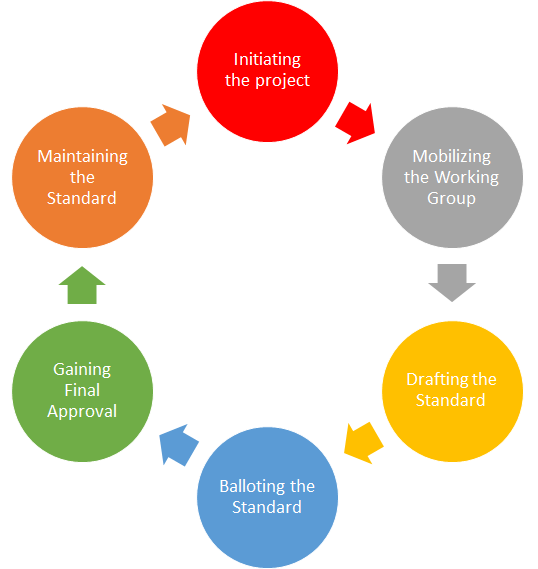
\includegraphics[width=0.7\linewidth]{Figures/Preface}
	\caption[Standardisation Process]{Standardisation Process}
	\label{fig:Standardisation_Process}
\end{figure}


\begin{enumerate}
	\item initiating the project

Although we have started in 2012 (Fleischmann et al., 2012) the needs for a standard has been identified 2 years ago. We started documenting (Referenz zu paper bei S-BPM 2019?) experiences from providers, users, researchers and system developers. Technological advancements in model execution have led to standardize the semantics, in order to reflect the novel opportunities. Once a need is identified, a proposal to create a new standard has to be put forward.

 \item  Mobilize a working group

Standards are created or reviewed by experts in the relevant field. They include researchers, providers, users and communities of practice, who form into a some technical committee, termed the Standardization Gang for subject orientation.

\item Balloting the standard by public review 

The technical committee conducts preliminary research and creates a draft outline of the new standard. Much of this initial work can be done remotely or in sub groups, however, needs to be consolidated at some point in time. This is where we are today when providing this edition of consolidated standard inputs.

\item Gain approval 

Once a draft is written, it requires approval for public review. This consensus is required in order to progress any further. The next step is to include all feedback and create a revised document for final public review. Thereby, anyone is welcome to provide feedback to improve the quality and ensure all relevant areas and perspectives are captured.

\item Publish and Maintain 

After public review, the standard goes back to the technical committee to make amendments it deems necessary based on the feedback received. The committee then approves the final version of the standard. After the revised standard receives that final approval from the technical committee, it is officially released. System developers or providers may incorporate it into their practice.

\end{enumerate}


The current version is intended for researcher who work in the area of software engineering and business process management. It helps understanding the approach through in-depth provision of the practical and theoretical aspects of subject oriented modeling and implementing systems.\\
The book is a collection of all the essential aspects of subject oriented modeling and programming. Many parts of this documents are reprints of various books and papers. Table \ref{tbl:sources} shows the sources for the various chapters and sections.\\
In chapter 1 an overview is given to the subject orientated language PASS and the methods which are used to describe its structural and execution semantics. OWl (Web Ontology Language) \cite{Web:OWL} is used to describe the structural semantics and Abstract State Machines (ASM) \cite{book:ASM-2018}, \cite{book:ASM-2003} is applied to specify the execution demantics precisely.\\
In chapter 2 the structure of PASS specification is considered in detail and its semantic is defined precisely in a formal way using OWL and ASM. The semantic of the execution of PASS models is described in chapter 3. The execution semantic uses coreASM which is an executable extension of the ASM method. This means that models described in PASS can be executed by a coresponding interpreter.\\
Chapter 4 shows how the abstract implementation independent PASS models can be implemented using software components, physical components or human.  A formal language is described how the right ressources are assigned to the entities of the model.\\
In the last chapter some additional aspects of the subject oriented modeling approach is considered. Thes aspects extend the kernel which was defined in chapter 2, 3 and 4.\\
The appendix contains the details of the formal semantic of PASS. Appendix A contains the complete Ontology, Abbendix B defines the mapping of the ontology to the ASM definition of PASS and Appendix C containes the complete formal execution semantics.



%\begin{longtable}
%	\footnotesize
%	\centering
%	\begin{tabular}[t]{@{}1 p{0.3\linewidth} p{0.3\linewidth} p{0.4\linewidth} @{}}
\todo[inline]{contact publisher for clarifying copyrights}
	\begin{longtable}[t]{ p{1 cm} p{4 cm} p{7 cm} }	
	\toprule
		\textbf{Chapter Nr.} & \textbf{Chapter title}  & \textbf{Source}
		\\
		\midrule
		1.1 \newline 2.1 \newline 3.1 & Subject Orientation and PASS \newline Informal Description \newline Informal Description of Subject Behaviour and its Execution & Fleischmann, Albert; Schmidt, Werner; Stary, Christian; Obermeier, Stefan; B\"orger, Egon; \newline \textit{Subject-Oriented Business Process Management,} \newline Springer Verlag Berlin 2012
		\\
		\midrule
		3.3 & ASM Definition of Subject Execution & 
		\\
		\midrule
		4.1 & People and Organisations & Fleischmann, Albert; Oppl, Stefan; Schmidt, Werner; Stary, Christian;\newline \textit{Contextual Process Digitalization: Changing Perspectives - Design Thinking - Value-Led Design} \newline Springer Verlag Berlin 2020
		\\
		\midrule
		5.1 & Subjects and Shared Input Pools & Fleischmann, A.; Stary, C.,\newline
			\textit{Dependable Data Sharing in Dynamic IoT-Systems - Subject-oriented Process Design, Complex Event Processing, and Blockchains;} \newline
			in Proceedings of S-BPM ONE 2019, 11th International Conference on Subject Oriented Business Process Management,\newline
			editors: Betz, S.;Elstermann, M.; Lederer, M; \newline
			ICPC published by Association of Computing Machinery (ACM) Digital Library; 2019
		\\
		\midrule
		5.2 & Subject-Phase Model based process specifications &  Fleischmann, A.,\newline
		\textit{Activity-Based Costing for S-BPM,}\newline
		Proceedings of the 5th International Conference S-BPM ONE 2013, Computer and Information Sciences (CCIS), No. 360,\newline
		editors: Fischer, H. and Schneeberger, J.\newline
		Springer 2013,
		\\
		\midrule
		5.3 & Hierarchies in Communication Oriented Business Process Models & Elstermann, M and Fleischmann, A.,\newline
		\textit{Modeling Complex Process Systems with Subject Oriebted Means,}\newline
		in Proceedings of S-BPM ONE 2019, 11th International Conference on Subject Oriented Business Process Management,\newline
		editors: Betz, S.;Elstermann, M.; Lederer, M; \newline
		ICPC published by Association of Computing Machinery (ACM) Digital Library; 2019
		\\
		\midrule
		5.4 & Business Activity Monitoring for S-BPM & Schmidt, W.; Fleischmann, A.;\newline
		\textit{Business Process Monitoring with S-BPM,}\newline
		Proceedings of the 5th International Conference S-BPM ONE 2013, Computer and Information Sciences (CCIS), No. 360,\newline
		editors: Fischer, H. and Schneeberger, J.\newline
		Springer 2013,
		\\
		\midrule
		5.5 & Subject Oriented Project Management & Albert Fleischmann, Werner Schmidt, Christian Stary;\newline
		\textit{Subject Oriented Project Management,}\newline
		published in SEAA '14: Proceedings of the 2014 40th EUROMICRO Conference on Software Engineering and Advanced Applications,\newline
		IEEE Computer Society, 2014
		\\
		\midrule
		5.6 & Subject Oriented Fog Computing & Stary, C. ; Fleischmann, A. ; Schmidt, W., \newline
		\textit{Subject-oriented Fog Computing: Enabling Stakeholder Participation in Development,} \newline
		Proceedings of the 4th IEEE World Forum on Internet of Things (WF-IoT), Singapure \newline
		IEEE Xplore Digital Library, DOI 10.1109/WF-IoT.2018.8355167, 2018
		\\
		\midrule
		5.6 & Activity Based Costeing &  Zehbold, C.; Schmidt, W.; Fleischmann, A.,\newline
		\textit{Activity-Based Costing for S-BPM,}\newline
		Proceedings of the 5th International Conference S-BPM ONE 2013, Computer and Information Sciences (CCIS), No. 360,\newline
		editors: Fischer, H. and Schneeberger, J.\newline
		Springer 2013,
		\\
\bottomrule
%\end{tabular}
\caption{Main sources of the various chapters and sections}
\label{tbl:sources}
\end{longtable}




\cleardoublepage

\setupparasubsecs
\setupmaintoc
\tableofcontents
\setlength{\unitlength}{1pt}
\cleardoublepage

%\listoffigures
%\clearpage
%\listoftables

%\lipsum{2}

%===================================

\mainmatter

% !TeX spellcheck = en_US

\chapter{Overview}

%\todo[inline]{
%Review CS: Chapter One should be a motivation including history of developements, \newline rationale and target reader groups (sntadarization bodies, developers, practitioners, researchers).
%\newline
%AF: See preface\\
%CS: Hochkommas und Bindestriche im pdf nicht alle lesbar, oft mt Umlauten gedruckt!
%}

To facilitate the understanding of the later sections, we will introduce the concept of subject-oriented process modeling with the modeling language Parallel Activity Specification Scheme (PASS). Additionally, we will give a short introduction to ontologies --- especially the Web Ontology Language (OWL) --- and to Abstract State Machines (ASM) as underlying concepts of this standard document.

\section{Subject Orientation and PASS}
\label{SubjectOrient} 

%\index{subject}

%\sidepar{Text in the sidebar}

In this section, we lay the ground for the Parallel Activity Specification Scheme (PASS) as a language for describing processes in a subject-oriented way. It will not a complete description of all PASS features, but it is a first impression and introduction to the principle of subject-orientation. The detailed concepts are defined in later chapters.

\subsubsection{The Term Subject in Subject-Orientation}
%\index{subject}

The term \textit{subject} has manifold meanings, depending on the discipline or domain it is used in. In philosophy, a subject is an observer and an object is a thing observed. In the grammar of many natural languages, the term subject has a slightly different meaning. "According to the traditional view, the [grammatical] subject is the doer of the action (actor) or the element that expresses what the sentence is about (topic)."~\cite{article:GeneralSubject}. In the English the term subject can also be used as a synonym for \textit{topic} as, e.g., the \textit{subject} of an e-mail. 

However, it is the first part of the second meaning that subject-orientation as a paradigm and PASS as a modeling language refer to in their concept. The term \textit{subject} corresponds to the concept of \textit{doer of an action}\footnote{In contrast to e.g. talks to e.g. ontology description languages, like RDF  (see section \ref{IntroOntology}), where term \textit{subject} means the topic what the "sentence" is about}.

\subsection{Subject-driven Business Processes}

In principle, subjects are the active entities in a specific process context that posses a behavior. A specification of a subject does not say anything about the technology used to execute the described behavior. This is different to other approaches, such as multi-agent systems, that usually imply a technical/software solution consisting of executable source code.

Subjects communicate with each other by exchanging information in form of \textit{messages}. Messages have a name and a payload. The name should express the topic or content of a message informally. The payload is the data (business objects) transported. 

During the execution of a (business) process, a subject sends messages to other subjects, expects messages from other subjects, and executes internal actions, such as calculating a price, storing an address, etc.. All these activities are done in sequences as no single processor or human can really multi-task. The possible sequence is defined in a subject's behavior specification. Subject-oriented process specifications are always embedded in a context. A context is defined by the business organization and the technology by which a business process\todo{Add glossary to the document} is executed.

Subject-oriented system development integrates established theories and concepts. It has been inspired by various process algebras (see e.g. [2], [3], [4]), by the basic structure of nearly all natural languages (Subject, Predicate, Object) and the systemic sociology developed by Niklas Luhmann (an introduction can be found in [5]). According to the organizational theory developed by Luhmann, the smallest organization consists of communication executed between at least two information processing entities[5]. 

\subsection{Subject-Orientation}

Consequently the term Subject-Orientation may be defined as following: 

Subject-Orientation is a modeling or description paradigm for processes that is derived from the structure of natural languages. It requires the explicit and continuous consideration of active entities within the bounds of a process as the conceptual center of description. Active entities (subjects) and passive elements (objects) must always be distinguished and activities or task can only be described in the context of a subject. The interaction between subjects is of particular importance and must explicitly be described as exchange of information that cannot be omitted \cite{elstermann:diss}

\subsection{PASS}

All the previously given concepts have been adapted into a simple graphical notation, that is the \textit{Parallel Activity Specification Schema} - or PASS . Following the principle of subject-orientation,the main concept of PASS is that, first the interaction between Subjects is described and only afterwards the behavior of subjects can be modeled individually. The details are given in the following sections.

\subsection{Modeling Subject Interaction}

We introduce the basic concepts of subject-oriented process modeling with a simple  \textit{order process}. In that process, a customer sends an \textit{order} to the order handling department of a supplier. He is going to receive an order confirmation and the ordered product by the shipment company. Figure \ref{fig:ordercomstructure1} shows the communication structure of that process. There all involved subjects and the exchanged messages can easily be discerned. 

%\strictpagecheck
\begin{figure}[htbp]
	\centering
	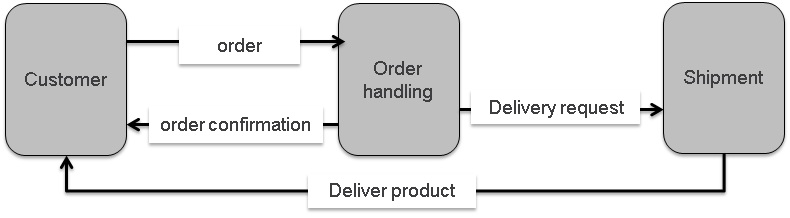
\includegraphics[width=0.7\linewidth]{Figures/Ontology/SubjectExecution/OrderComStructure}
	\caption[The Communication Structure of a simple Order Process]{The Communication Structure of a simple Order Process}
	\label{fig:ordercomstructure1}
\end{figure}

It is assumed that  each subject has a so-called \textit{input pool} which is basically its mailbox for receiving messages. This input pool can be structured via rules according to the requirements in given process context. The modeler can define how many messages of which type and/or from which sender can be deposited and what the reaction is if these restrictions are violated. This means the synchronization through message exchange can be specified for each subject individually.

Messages should have their meaning expressed by their name. A formal semantics is given by their use and the data which are transported with a message. 


\subsection{Modeling Subject Behavior}

Figure \ref{fig:ordercustomerorderhandling} depicts the behavior of the subjects "customer" and "order handling".

%\strictpagecheck
\begin{figure}[htbp]
	\centering
	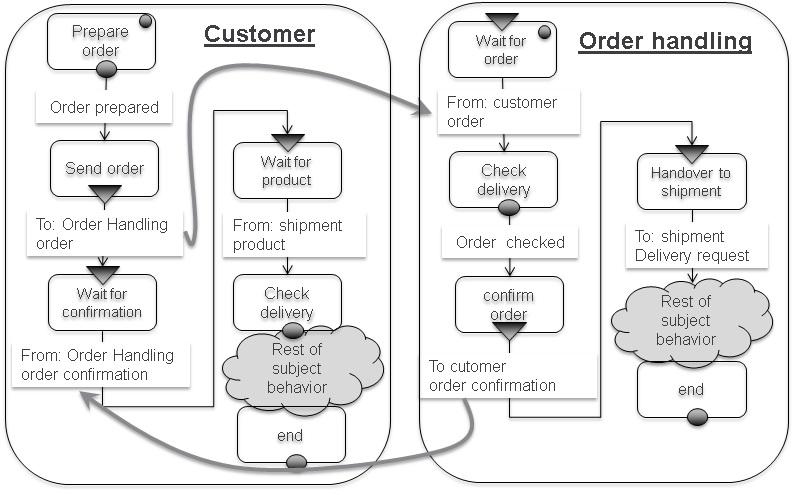
\includegraphics[width=0.9\linewidth]{Figures/Ontology/SubjectExecution/OrderCustomerOrderHandling}
	\caption[The Behaviors of the Subjects from \ref{fig:ordercomstructure1} ]{The Behaviors of the Subjects from \ref{fig:ordercomstructure1}}
	\label{fig:ordercustomerorderhandling}
\end{figure}

In the first state (Do State) of its behavior, the subject "customer" executes the \textit{internal function}  "Prepare order". When this function is finished the transition "order prepared" follows. It basically states the condition that must be fulfilled in order to continue. In the succeeding (Send) state "send order" the message "order" is sent to the subject "order handling". After this message is sent (deposited in the input pool of subject "order handling"), the subject "Customer" is allowed to go into the (Receive) state "wait for confirmation". If this message is not in the input pool the subject stops its execution until the corresponding message arrives in the input pool and the according receive transition condition is fulfilled. On arrival, the subject removes the message from the input pool and follows the transition into state "Wait for product" and so on.

The subject "Order Handling" waits for the message "order" from the subject "customer". If this message is in the input pool it is removed and the succeeding function "check order" is executed and so on.

In summary, the behavior of each subject describes in which order it sends and receives (expects) messages, and performs internal functions. Messages transport data from the sending to the receiving subject and internal functions operate on internal data of a subject. These data aspects of a subject are described in section \ref{SUbjects-Objects}. 

%\subsection{Advanced Subject Behavior Modeling}

%In a dynamic and fast-changing world, processes need to be able to capture known but unpredictable events. In our example let us assume that a customer can change an order. This means the subject "customer" may send the message "Change order" at any time. Figure\todo{AF: Bild und Text passen nicht Change order} \ref{fig:ordercomstructure2} shows the corresponding communication structure, which now contains the message "change order".

%%\strictpagecheck
%\begin{figure}[htbp]
%	\centering
%	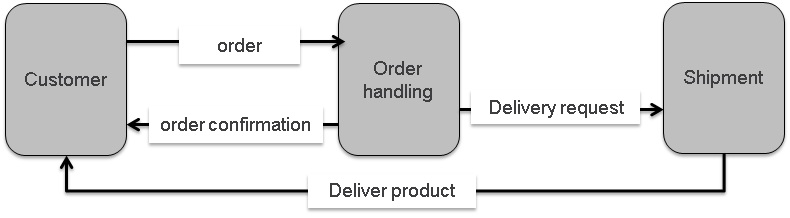
\includegraphics[width=0.7\linewidth]{Figures/Ontology/SubjectExecution/OrderComStructure}
%	\caption[The Communication Structure with Change Message]{The Communication Structure with Change Message}
%	\label{fig:ordercomstructure2}
%\end{figure}

%Due to this unpredictable event, the behavior of the involved subjects needs also to be adapted. Figure \ref{fig:ordercustomerchange} illustrates the respective behavior of the customer. 

%\strictpagecheck
%\begin{figure}[htbp]
%	\centering
%	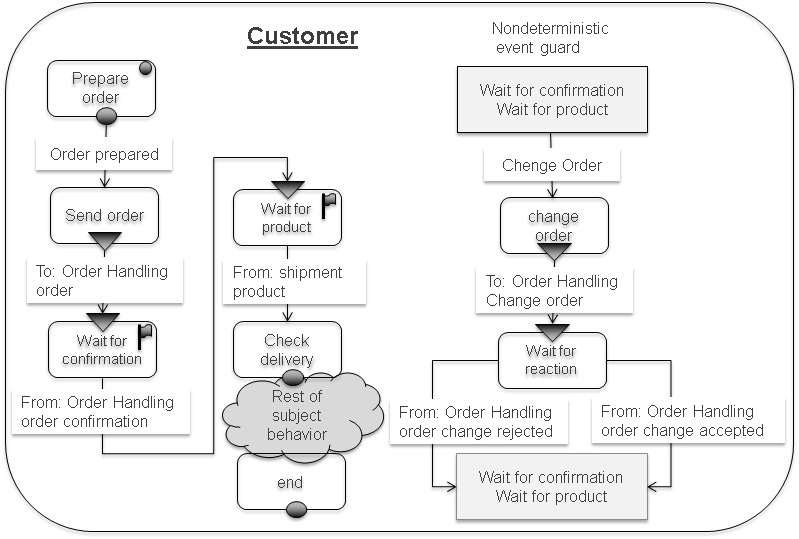
\includegraphics[width=0.9\linewidth]{Figures/Ontology/SubjectExecution/OrderCustomerChange}
%	\caption[Customer is allowed to Change Orders]{Customer is allowed to Change Orders}
%	\label{fig:ordercustomerchange}
%\end{figure}

%The subject "customer" may have the idea to change its order in the state "wait for confirmation" or in the state "wait for product". The flags in these states indicate that there is a so-called behavior extension described by a so-called nondeterministic event guard [12, 22]. The non-deterministic event created in the subject is the idea "change order". If this idea comes up, the current states, either "wait for confirmation" or "wait for product", are left, and the subject "customer" jumps into state "change order" in the guard behavior. In this state, the message "change order" is sent and the subject waits in the state "wait for reaction". In this state, the answer can either be "order change accepted" or "order change rejected". Independently of the received message the subject "customer" moves to the state "wait for product". The message "order change accepted" is considered as confirmation, if a confirmation has not arrived yet (state "wait for confirmation"). If the change is rejected the customer has to wait for the product(s) he/she has ordered originally. Similar to the behavior of the subject "customer" the behavior of the subject "order handling" has to be adapted.

\subsection{Subjects and Data}
\label{SUbjects-Objects}

Up to now, we did not explicitly mention data or rather the concept of data, even though they are necessary to get complete sentences comprising subject, predicate (verbs), and object. In subject-orientation (data-)objects have their place\footnote{Theoretically, the means subject-oriented modeling and object-oriented modeling are 100\% compatible In regards to natural languages it must be understood that pure object-oriented means are akin the passive sentence structures where the subject may be omitted, while subject-oriented descriptions follow the structure of active sentences, that are much easier to understand. }


It is assumed that each subject posses an individual "database" to allow to store objects of arbitrary complexity. Similarly, messages may have a data \textit{payload} representing the transport of data between subjects.
Figure \ref{fig:subjectobject} displays how subjects and objects are connected in the classical way. The internal function  "prepare order" uses or manipulates internal data to prepare the data for the order message. This order data object is sent as the \textit{payload} of the message "order".

%\strictpagecheck
\begin{figure}[htbp]
	\centering
	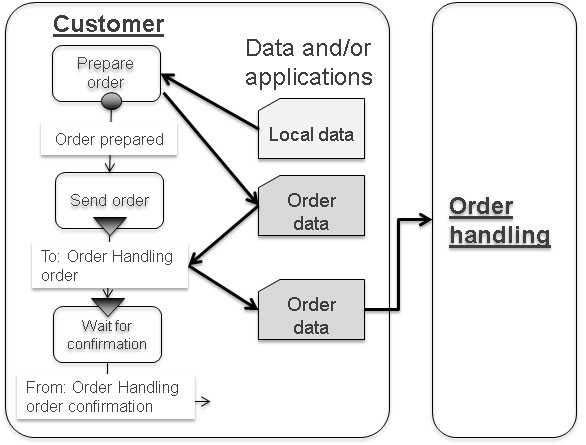
\includegraphics[width=0.9\linewidth]{Figures/Ontology/SubjectExecution/SUbjectObject}
	\caption[Subjects and (Data-)Objects]{Subjects and (Data-)Objects}
	\label{fig:subjectobject}
\end{figure}


Modeling wise, internal functions in a subject can be described as the (passive) methods of a specific data-object or as function calls implemented in a service, if a service-oriented architecture is available.

The functions of send and receive states are assumed to always have an additional method that transfer data between messages and internal data store of a subject. If a message is sent, the method writes data values into to the sent message, and if a message is received the corresponding method is used to copy the received data into the subject's data store [22]. In other words, subject either use synchronous services as an implementation of functions, or asynchronous services that are implemented through other subjects or even through complex processes consisting of multiple subjects themselves. Consequently, the concept Service Oriented Architecture (SOA) is complementary to S-BPM: Subjects are the entities which use the services offered by SOAs (cf. [25]).

\section{Introduction to Ontologies and OWL }
\label{IntroOntology}

This short introduction to ontology, the Resource Description Framework (RDF), and the Web Ontology Language (OWL) will help to get an understanding of their usage as definition technologies for Subject-Oriented Modeling and Implementation standard in the form of the PASS ontology that is outlined in sections \ref{PASSStruct} and \ref{PASSExec}.

Ontologies are a formal collections of knowledge or descriptions about the world. They are being used to structure the knowledge of  various domains using taxonomies and classification networks. They often use structures similar to human languages, where nouns in statement-sentences represent objects or classes of objects and the verbs represents relations between the objects of classes. (e.g. \textit{"PASS" "is-a" "process modeling language"})

In computer- and information science, an ontology is a collection or representation of formal names, class definitions, properties, relations between them, and according entities with their relations  - usually in regards to a specific thematic domain.


\subsection{RDF and OWL}

The Resource Description Framework (RDF)\cite{rdf:rdf} provides a graph-based data model or framework for structuring data as statements about resources. A "resource" may be any "thing" that exists in the world: a person, place, event, book, museum object, but also an abstract concept like data objects. Figure \ref{fig:classes-properties}  shows an RDF graph.

%\strictpagecheck
\begin{figure}[h]
	\centering
	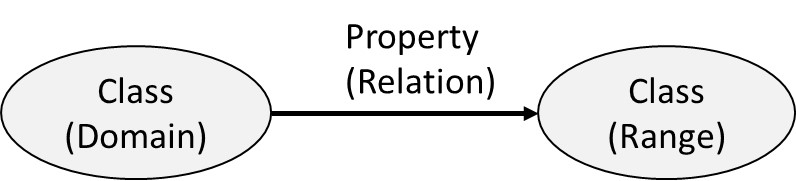
\includegraphics[width=0.6\linewidth]{Figures/Ontology/Introduction/Classes-Properties}
	\caption[RDF graphic]{RDF graphic}
	\label{fig:classes-properties}
\end{figure}

RDF is based on the idea of making statements about resources (in particular web resources) in expressions of the form subject–predicate–object, known as triples. The subject denotes the resource, and the predicate denotes traits or aspects of the resource and expresses a relationship between the subject and the object. In the context of ontology, the term subject expresses what the sentence is about (topic), it must not be confused with term subject in the context of Subject-Orientation (see \ref{SubjectOrient}).

For describing ontologies several formal languages have been developed. One widely used language is OWL (Web Ontology Language)\cite{w3c:owl}, which is based on, or a kind of extension to the Resource Description Framework (RDF).

OWL introduces and allows to use the modeling mechanisms of classes, properties, and instances. Classes represent terms also called concepts. Classes have properties and instances are individuals of one or more class.

A class is a type of thing. A type of "resource" in the RDF sense can be a person, place, object, concept, event, etc.. Classes and subclasses form a hierarchical taxonomy and members of a subclass inherit the characteristics of their parent class (superclass). Everything true for the parent class is also true for the subclass. A member of a subclass "is a", or "is a kind of" its parent class.

OWL Ontologies define a set of properties used in a specific knowledge domain. In an ontology context, properties relate members of one class to members of another class or a literal.

Domains and ranges define restrictions on properties. A domain restricts what kinds of resources or members of a class can be the subject of a given property in an RDF triple. A range restricts what kinds of resources/members of a class or data types (literals) can be the object of a given property in an RDF triple.

Entities belonging to a certain class are instances of this class or individuals. A simple ontology with various classes, properties and individual is shown below:

\subsubsection{Ontology statement examples:}

\begin{itemize}
	\item \textbf {Class definition statements:}
	\begin{itemize}
		\item Parent \texttt{isA} Class
		\item Mother \texttt{isA} Class
		\item Mother \texttt{subClassOf} Parent
		\item Child \texttt{isA} Class
	\end{itemize}
	\item \textbf {Property definition statement:}
	\begin{itemize}
		\item \texttt{isMotherOf} is a relation between the classes Mother and Child
	\end{itemize}
	\item \textbf{Individual/instance statements:}
	\begin{itemize}
		\item MariaSchmidt \texttt{isA} Mother
		\item MaxSchmidt \texttt{isA} Child
		\item MariaSchmidt \texttt{isMotherOf} MaxSchmidt
	\end{itemize}
\end{itemize}

\section{Introduction to Abstract State Machines}

Where the OWL/RDF ontology concepts will be used to define the static structure of subject-oriented process models. The execution semantics will be specified using the concept of \textit{Abstract State Machines}. This section will give a short introduction into this topic in order to help the understanding of their usage in section \ref{PASSExec}.

An abstract state machine (ASM) is a state machine\footnote{State Machines and therefore also abstract state machines are both formal description concepts in theoretical computer science used to describe or define the execution order of a system - e.g. a software program} operating on states that are arbitrary data structures (structure in the sense of mathematical logic, that is a nonempty set together with several functions (operations) and relations over the set). In simpler terms, where in standard state machines the states are explicitly defined (e.g. \textit{state01}, \textit{state02}), in an ASM the states or only implicitly or abstractly defined (e.g. \textit{"a state where a data value is x"}).

The language of the so-called Abstract State Machine uses only elementary If-Then-Else-rules which are typical also for rule systems formulated in natural languages, i.e., rules of the (symbolic) form:

\medskip
$\boldsymbol{if} \textit{Condition} \boldsymbol{then} \textit{ACTION}$
\medskip

with arbitrary \textit{Condition} and \textit{ACTION}. The latter is usually a finite set of assignments of the form \textit{f (t1, ..., tn) := t}. The meaning of such a rule is to be performed in any given state, when the indicated condition holds true - the \textit{CONDITION} there indirectly defines that state.

The unrestricted generality of the used notion of \textit{CONDITION} and \textit{ACTION} is guaranteed by using so-called Tarski structures as ASM-states, i.e., arbitrary sets of arbitrary elements with arbitrary functions and relations defined on them. These structures are not necessarily fixed, but are themselves updatable by rules of the form above. 

%In the case of business processes, the elements of \textit{CONDITION} and \textit{ACTION}-rules are placeholders for values of arbitrary type and the operations are typically the creation, duplication, deletion, or manipulation (value change) of objects. The so-called views are conceptually nothing else than projections (read: substructures) of such Tarski structures.

An (asynchronous or distributed) ASM consists of a set of agents, each equipped with an individual set of rules in the above given form, called its program. In principle, every agent can evaluated and , if applicable, execute all its rules at any time in one step (in any arbitrary state). In contrast, an ASM, that has only one agent, is called sequential ASM. In general, each agent has its own "time" to execute a step, and a step is independent of the steps of other agents. However there in special cases, multiple agents can also execute their steps in a synchronous manner.

Without further explanations, we adopt usual notations, abbreviations, etc., for example:

% for the typesetting of ASM code some work is required!!
%\lstdefinelanguage{ASM}{C}
%\lstset{language=ASM}
\medskip
$ \mathbf{if} ~ Cond  ~ \mathbf{then} ~ M1 ~ \mathbf{else} ~ M2$
\medskip

instead of the equivalent ASM with two rules:

\medskip
$ \mathbf{if} ~ Cond  ~ \mathbf{then}  M1$
$ \mathbf{if ~ not} ~ Cond  ~ \mathbf{then} ~ M2$
\medskip

Another notation used below is

\medskip
$ \mathbf{let} ~ x ~ = ~ t ~ \mathbf{in} ~ M$
\medskip

for $M(x/a)$, where $a$ denotes the value of $t$ in the given state and $M(x/a)$ is obtained from $M$ by substitution of each (free) occurrence of $x$ in $M$ by $a$.

For details of a mathematical definition of the semantics of ASMs which justifies their intuitive (rule-based or pseudo-code) understanding, we refer the reader to the AsmBook Börger, E., Stärk R. Abstract State Machines. A Method for High-Level System Design and Analysis. Springer, 2003 \cite{book:ASM-2003}.






% Review Christia Stary January 2020

\chapter{Structure of a PASS Description}
\label{PASSStruct}

In this chapter, we describe the structure of a PASS specification. The structure of a PASS description consists of the subjects and the messages they exchange.

\emph{\underline{\textit{\textbf{Review CS: In this chapter, concepts are presented, that are not all part of the diagrammatic representation (SIDs or BDs). It should be somewhere noted that modeling and runtine knowledge, in particular about the input pool, has to be acquired in textual form when using the specification scheme. So, standardizing the PASS description contains of text and diagrams.}}}}

\section{Informal Description}
\subsection{Subject}
\label{sec: Subject}

As already detailed previously, subjects represent the behavior of an active entity. A specification of a subject does not say anything about the technology used to execute the described behavior. Subjects communicate with each other by exchanging messages. Messages have a name and a payload. The name should express the meaning of a message informally and the payloads are the data (business objects) transported. Internal subjects execute local activities such as calculating a price, storing an address, etc. External subjects represent interfaces for other business processes.

CS: would it not be more convenient to move the conceptual understanding to section 1.1 and then just refer to this part, instead of rephrasing the same concept several times?

A subject sends messages to other subjects, receives messages from other subjects, and executes internal actions. All these activities are done in logical order which is defined in a subject's behavior specification.

In the following, we use an example of the informal definition of subjects. In the simple scenario of the business trip application, we can identify three subjects, namely the employee as the applicant, the manager as the approver, and the travel office as the travel arranger.

In general, there are the following types of subjects:

\begin{itemize}
	\item Fully specified subjects
	\item Multi-subjects
	\item Single subjects
	\item Interface subjects 
\end{itemize}

\subsubsection{Fully specified Subjects}

This is the standard subject type. A subject communicates with other subjects by exchanging messages. Fully specified subjects consist of the following components:

\begin{itemize}
	\item Business Objects---Each subject has some business objects. A basic structure of business objects consists of an identifier, data structures, and data elements. The identifier of a business object is derived from the business environment in which it is used. Examples are business trip requests, purchase orders, packing lists, invoices, etc. Business objects are composed of data structures. Their components can be simple data elements of a certain type (e.g., string or number) or even data structures themselves. 
	\item Sent messages---Messages which a subject sends to other subjects. Each message has a name and may transport some data objects as a payload. The values of these payload data objects are copied from internal business objects of a subject.
	\item Received messages---Messages received by a subject. The values of the payload objects are copied to business objects of the receiving subject.
	\item Input Pool---Messages sent to subjects are deposited in the input pool of the receiving subject. The input pool is a very important organizational and technical concept in this case.
	\item Behavior---The behavior of each subject describes in which logical order it sends messages, expects (receives) messages, and performs internal functions. Messages transport data from the sending to the receiving subject and internal functions operate on internal data of a subject. 
\end{itemize}


\subsubsection{Multsubjects and Multiprocesses}

Multi-subjects are similar to fully specified subjects. If in a process model several identical subjects are required, e.g. to increase the throughput, this requirement can be modeled by a multi-subject. If several communicating subjects in a process model are multi-subjects they can be combined to a multi-process.

In a business process, there may be several identical sub-processes that perform certain similar tasks in parallel and independently. This is often the case in a procurement process when bids from multiple suppliers are solicited. A process or sub-process is therefore executed simultaneously or sequentially multiple times during overall process execution. A set of type-identical, independently running processes or sub-processes is termed multi-process. The actual number of these independent sub-processes is determined at runtime.

Multi-processes simplify process execution since a specific sequence of actions can be used by different processes. They are recommended for recurring structures and similar process flows. 

An example of a multi-process can be illustrated as a variation of the current booking process. The travel agent should simultaneously solicit up to five bids before making a reservation. Once three offers have been received, one is selected and a room is booked. The process of obtaining offers from the hotels is identical for each hotel and is therefore modeled as a multi-process.

\subsubsection{Single subjects}

Single subjects can be instantiated only once. They are used if for the execution of a subject a resource is required which is only available once.

\subsubsection{Interface Subjects}

Interface subjects are used as interfaces to other process systems (CS: this term needs explanation or other wording, e.g., "other context"). If a subject of a process system sends or receives messages from a subject which belongs to another workflow system. These so-called interface subjects represent fully described subjects which belong to that other process system. Interface subjects specifications contain the sent messages, received messages and the reference to the fully described subject which they represent.

\subsection{Subject-to-Subject Communication}

After the identification of subjects involved in the process (as process-specific roles), their interaction relationships need to be represented. These are the messages exchanged between the subjects. Such messages might contain structured information—so-called business objects.

The result is a model of the communication relationships between two or more subjects, which is referred to as a \textbf{Subject Interaction Diagram} (SID) or, synonymously, as a Communication Structure Diagram (CSD) (see figure \ref{fig:beispiel-SubjectInteraction}).

\begin{figure*}[htbp]
	\centering
	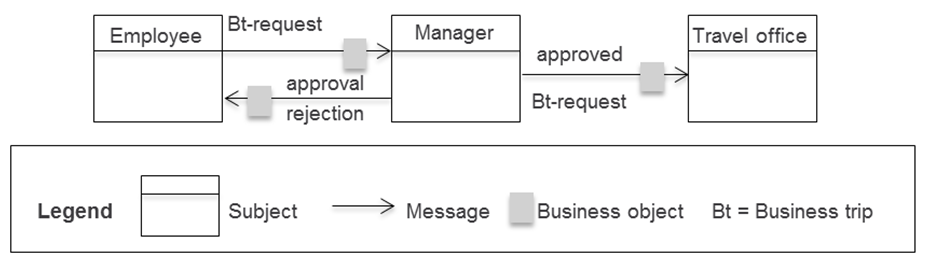
\includegraphics[width=14cm]{Figures/Ontology/SubjectInteraction/Beispiel-Subject-Interaction.png}
	\caption[Subject interaction diagram]{Subject interaction diagram for the process 'business trip application'}
	\label{fig:beispiel-SubjectInteraction}
\end{figure*}

Messages represent the interactions of the subjects during the execution of the process. We recommend naming these messages in such a way that they can be immediately understood and also reflect the meaning of each particular message for the process. In the sample 'business trip application', therefore, the messages are referred to as 'business trip request', 'rejection', and 'approval'.

Messages serve as a container for the information transmitted from a sending to a receiving subject. There are two options for the message content:

\begin{itemize}
	\item     Simple data types---Simple data types are string, integer, character, etc. In the business trip application example, the message 'business trip request' can contain several data elements of type string (e.g., destination, the reason for traveling, etc.), and of type number (e.g., duration of the trip in days).
	\item Business Objects---Business Objects in their general form are physical and logical 'things' that are required to process business transactions. We consider data structures composed of elementary data types, or even other data structures, as logical business objects in business processes. For instance, the business object 'business trip request' could consist of the data structures 'data on applicants', 'travel data', and 'approval data' with each of these in turn containing multiple data elements.
\end{itemize}

\subsection{Message Exchange}

In the previous subsection, we have stated that messages are transferred between subjects and have described the nature of these messages. What is still missing is a detailed description of how messages can be exchanged, how the information they carry can be transmitted, and how subjects can be synchronized. These issues are addressed in the following sub-sections.

\subsubsection{Synchronous and Asynchronous Exchange of Messages}

In the case of an synchronous exchange of messages, sender and receiver wait for each other until a message can be passed on. If a subject wants to send a message and the receiver (subject) is not yet in a corresponding receive state, the sender waits until the receiver can accept this message. Conversely, a recipient has to wait for the desired message until it is made available by the sender.

The disadvantage of the synchronous method is a close temporal coupling between sender and receiver. This raises problems in the implementation of business processes in the form of workflows, especially across organizational borders. As a rule, these also represent system boundaries across which a tight coupling between sender and receiver is usually very costly. For long-running processes, sender and receiver may wait for days, or even weeks, for each other.

Using asynchronous messaging, a sender can send anytime. The subject puts a message into a message buffer from which it is picked up by the receiver. However, the recipient sees, for example, only the oldest message in the buffer (in case the buffer is implemented as FIFO or LIFO storage) and can only accept this particular one. If it is not the desired message, the receiver is blocked, even though the message may already be in the buffer, but in a buffer space that is not visible to the receiver. To avoid this, the recipient has the alternative to take all of the messages from the buffer and manage them by himself. In this way, the receiver can identify the appropriate message and process it as soon as he or she needs it. In asynchronous messaging, sender and receiver are only loosely coupled. Practical problems can arise due to the in reality limited physical size of the receive buffer, which does not allow an unlimited number of messages to be recorded. Once the physical boundary of the buffer has been reached due to high occupancy, this may lead to unpredictable behavior of workflows derived from a business process specification. To avoid this, the input-pool concept has been introduced in PASS. Nevertheless, the number of messages must always be limited, as a business process must have the capacity to handle all messages to maintain some sort of service level.


\subsubsection{Exchange of Messages via the Input Pool}
\label{sec: inputpool}

To solve the problems outlined in the asynchronous message exchange, the input pool concept has been developed. Communication via the input pool is considerably more complex than previously shown; however, it allows transmitting an unlimited number of messages simultaneously. Due to its high practical importance, it is considered as a basic construct of PASS.

Consider the input pool as a mailbox of work performers, the operation of which is specified in detail. Each subject has its input pool. It serves as a message buffer to temporarily store messages received by the subject, independent of the sending communication partner. The input pools are therefore inboxes for flexible configuration of the message exchange between the subjects. In contrast to the buffer in which only the front message can be seen and accepted, the pool solution enables picking up (i.e. removing from the buffer) any message. For a subject, all messages in its input pool are visible.

The input pool has the following configuration parameters (see figure \ref{fig:input-pool}):

\begin{itemize}
	\item Input-pool size---The input-pool size specifies how many messages can be stored in an input pool, regardless of the number and complexity of the message parameters transmitted with a message. If the input pool size is set to zero, messages can only be exchanged synchronously.
	\item Maximum number of messages from specific subjects---For an input pool, it can be determined how many messages received from a particular subject may be stored simultaneously in the input pool. Again, a value of zero means that messages can only be accepted synchronously.
	\item Maximum number of messages with specific identifiers---For an input pool, it can be determined how many messages of a specifically identified message type (e.g., invoice) may be stored simultaneously in the input pool, regardless of what subject they originate from. A specified size of zero allows only for synchronous message reception.
	\item Maximum number of messages with specific identifiers of certain subjects---For an input pool, it can be determined how many messages of a specific identifier of a particular subject may be stored simultaneously in the input pool. The meaning of the zero value is analogous to the other cases.
\end{itemize}

\begin{figure*}[htbp]
	\centering
	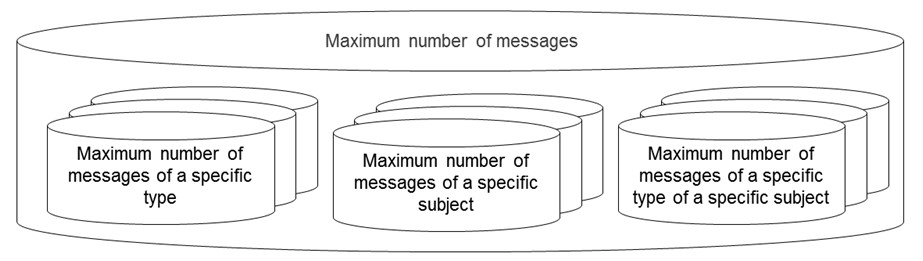
\includegraphics[width=12cm]{Figures/Ontology/SubjectInteraction/input-pool-informal.jpg}
	\caption[Input Pool]{Configuration of Input Pool Parameters}
	\label{fig:input-pool}
\end{figure*}

By limiting the size of the input pool, its ability to store messages may be blocked at a certain point in time during process runtime. Hence, messaging synchronization mechanisms need to control the assignment of messages to the input pool. Essentially, there are three strategies to handle access to input pools:

\begin{itemize}
	\item Blocking the sender until the input pool’s ability to store messages has been reinstated---Once all slots are occupied in an input pool, the sender is blocked until the receiving subject picks up a message (i.e. a message is removed from the input pool). This creates space for a new message. In case several subjects want to put a message into a fully occupied input pool, the subject that has been waiting longest for an empty slot is allowed to send. The procedure is analogous if corresponding input pool parameters do not allow storing the message in the input pool, i.e., if the corresponding number of messages of the same name or from the same subject has been put into the input pool.
	\item Delete and release of the oldest message---In case all the slots are already occupied in the input pool of the subject addressed, the oldest message is overwritten with the new message.
	\item Delete and release of the latest message---The latest message is deleted from the input pool to allow depositing of the new incoming message. If all the positions in the input pool of the addressed subject are taken, the latest message in the input pool is overwritten with the new message. This strategy applies analogously when the maximum number of messages in the input pool has been reached, either concerning sender or message type.
\end{itemize}

\section{OWL Description}
\label{OWL-DescriptionSID}

\underline{\textit{\textbf{Übergang von informeller zur formalen Beschreibung sehr abrupt und unverstaändlich}}}




The various building blocks of a PASS description and their relations are defined in an ontology. The following figure \ref{fig:20171217-passprocessmodellelement} gives an overview of the structure of the PASS specifications.  

 
 \underline{\textit{\textbf{Nummerierung erklären, Wie kommen Nummern zustande}}}


\begin{figure*}[htbp]
	\centering
	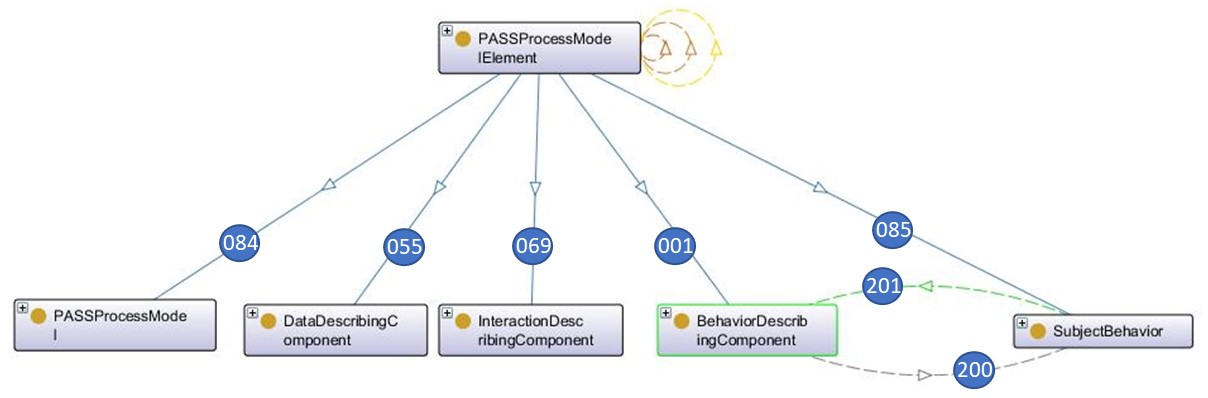
\includegraphics[width=0.9\linewidth]{Figures/Ontology/SubjectInteraction/20171217-PASSProcessModellElement}
	\caption[Elements of PASS Process Models]{Elements of PASS Process Models}
	\label{fig:20171217-passprocessmodellelement}
\end{figure*}

The class \texttt{PASSProcessModelElement} has five subclasses (subclass relations 084, 055, 069, 001 and 085 in figure \ref{fig:20171217-passprocessmodellelement}). Only the classes \texttt{PASSProcessModel}, \texttt{DataDescriptionCOmponent}, \texttt{InteractionDescribingComponent} are used for defining the structural aspects of a process specification in PASS. The classes \texttt{BehaviorDescribingComponent} and \texttt{SubjectBehavior} define the dynamic aspects, namely in which sequences messages are sent and received or internal actions are executed. These dynamic aspects are considered in detail in the next chapter. 

\subsection{PASS Process Model}

The central entities of a PASS process model are subjects which represent the active elements of a process and the messages they exchange. Messages transport data from one subject to others (payload). Figure \ref{fig:20181217-passprocessmodel} shows the corresponding ontology for the PASS process models.

\begin{figure*}[htbp]
	\centering
	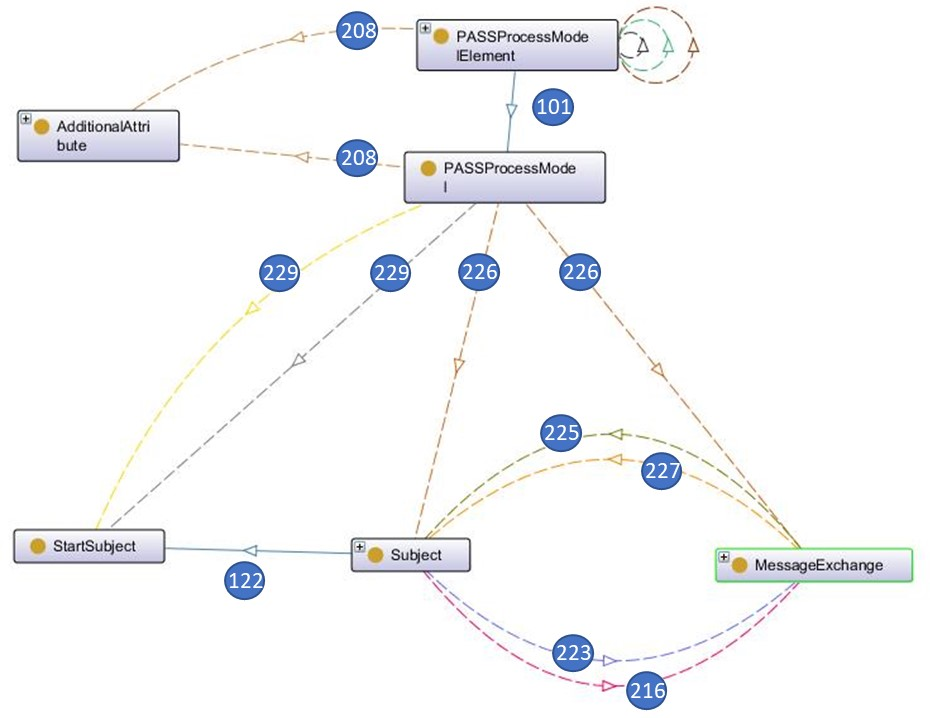
\includegraphics[width=1.0\linewidth]{Figures/Ontology/SubjectInteraction/20181217-PASSProcessModel}
	\caption[PASS Process Modell]{PASS Process Modell}
	\label{fig:20181217-passprocessmodel}
\end{figure*}

\texttt{PASSProcessModelElements} and \texttt{PASSProcessModells} have a name. This is described with the property \texttt{hasAdditionalAttribute} (property 208 in \ref{fig:20171217-passprocessmodellelement}). The class subject and the class \texttt{MessageExchange} have the relation \texttt{hasRelation} \texttt{toModelComponent} to the class \texttt{PASSProcessModel} (property 226 in \ref{fig:20171217-passprocessmodellelement}). The properties \texttt{hasReceiver} and \texttt{hasSender} express that a message has a sending and receiving subject (properties 225 and 227 in \ref{fig:20171217-passprocessmodellelement}) whereas the properties \texttt{hasOutgoingMessageExchange} and \texttt{hasIncomingMessageExchange} define which messages are sent or received by a subject. Property \texttt{hasStartSubject} (property 229 in \ref{fig:20171217-passprocessmodellelement}) defines a start subject for a \texttt{PASSProcessModell}. A start subject is a subclass of the class subject (subclass relation 122 in \ref{fig:20171217-passprocessmodellelement}).

\subsection{Data Describing Component}

Each subject encapsulates data (business objects). The values of these data elements can be transferred to other subjects. The following figure \ref{fig:20181218-data} shows the ontology of this part of the PASS-ontology.

\begin{figure}[htbp]
	\centering
	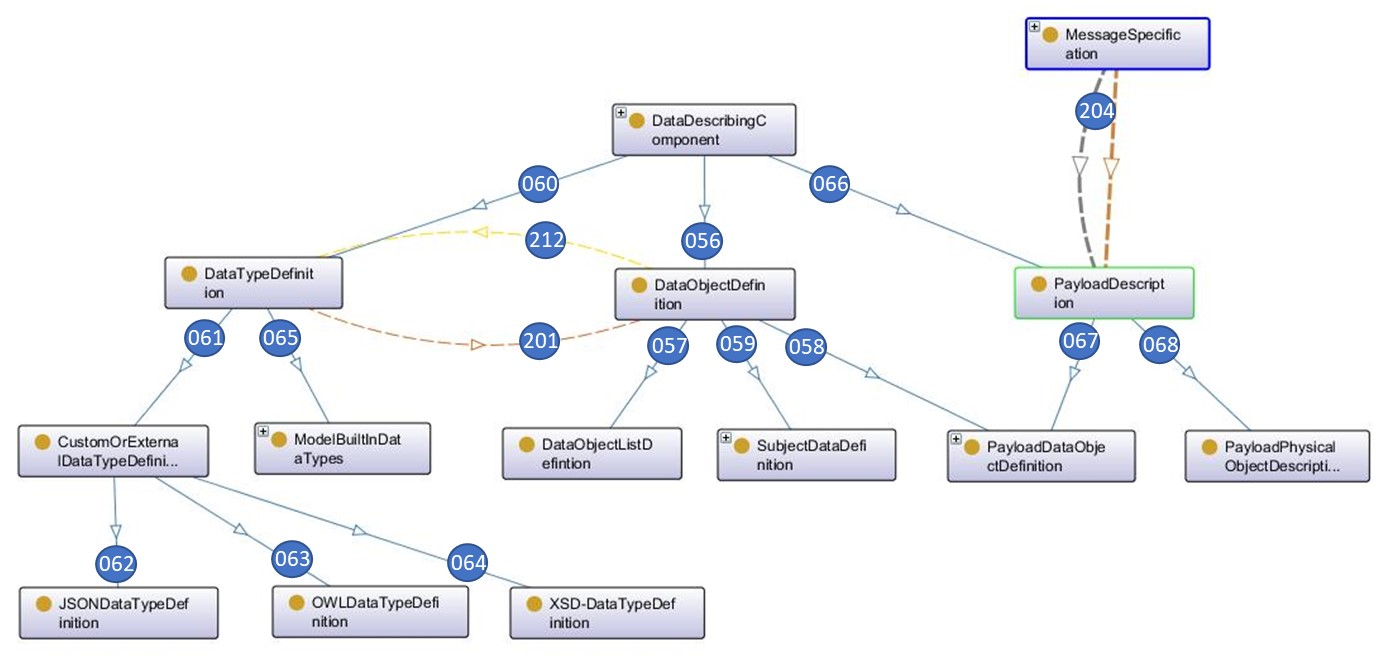
\includegraphics[width=0.9\linewidth]{Figures/Ontology/SubjectInteraction/20181218-Data}
	\caption[Data Description Component]{Data Description Component}
	\label{fig:20181218-data}
\end{figure}

Three subclasses are derived from the class \texttt{DtadescribingComponent} (in figure \ref{fig:20181218-data} are these the relations 060, 056 and 066). The subclass \texttt{PayLoadDescription} defines the data tranported by messages. The relation of \texttt{PayloadDescriptions} to messages is defined by the property \texttt{ContainsPayloadDescription} (in figure \ref{fig:20181218-data} number 204).

There are two types of payloads. The class \texttt{PayloadPhysicalObjectDescription} is used if a message will be later implemented by a physical transport like a parcel. The class \texttt{PayLoadDataObjectDefinition} is used to transport normal data (Subclass relations 068 and 67 in figure \ref{fig:20181218-data}). These payload objects are also a subclass of the class \texttt{DataObjectDefinition} (Subclass relation 058 in figure \ref{fig:20181218-data}).

Data objects have a certain type. Therefore class \texttt{DataObjectDefinition} has the relation \texttt{hasDatatype} to class \texttt{DataTypeDefinition} (property 212 in figure\ref{fig:20181218-data}). Class \texttt{DataTypeDefinition} has two subclasses (subclass relations 061 and 065 in figure \ref{fig:20181218-data}). The subclass \texttt{ModelBuiltInDataTypes} are user defined data types whereas the class \texttt{CustomOfExternalDataTypeDefinition} is the superclass of JSON, OWL or XML based data type definitions(subclass relations 062, 63 and 064 in figure \ref{fig:20181218-data}).

\subsection{Interaction Describing Component}

The following figure \ref{fig:ontogrsubjectinteraction} shows the subset of the classes and properties required for describing the interaction of subjects. 

\begin{figure*}[htbp]
	\centering
	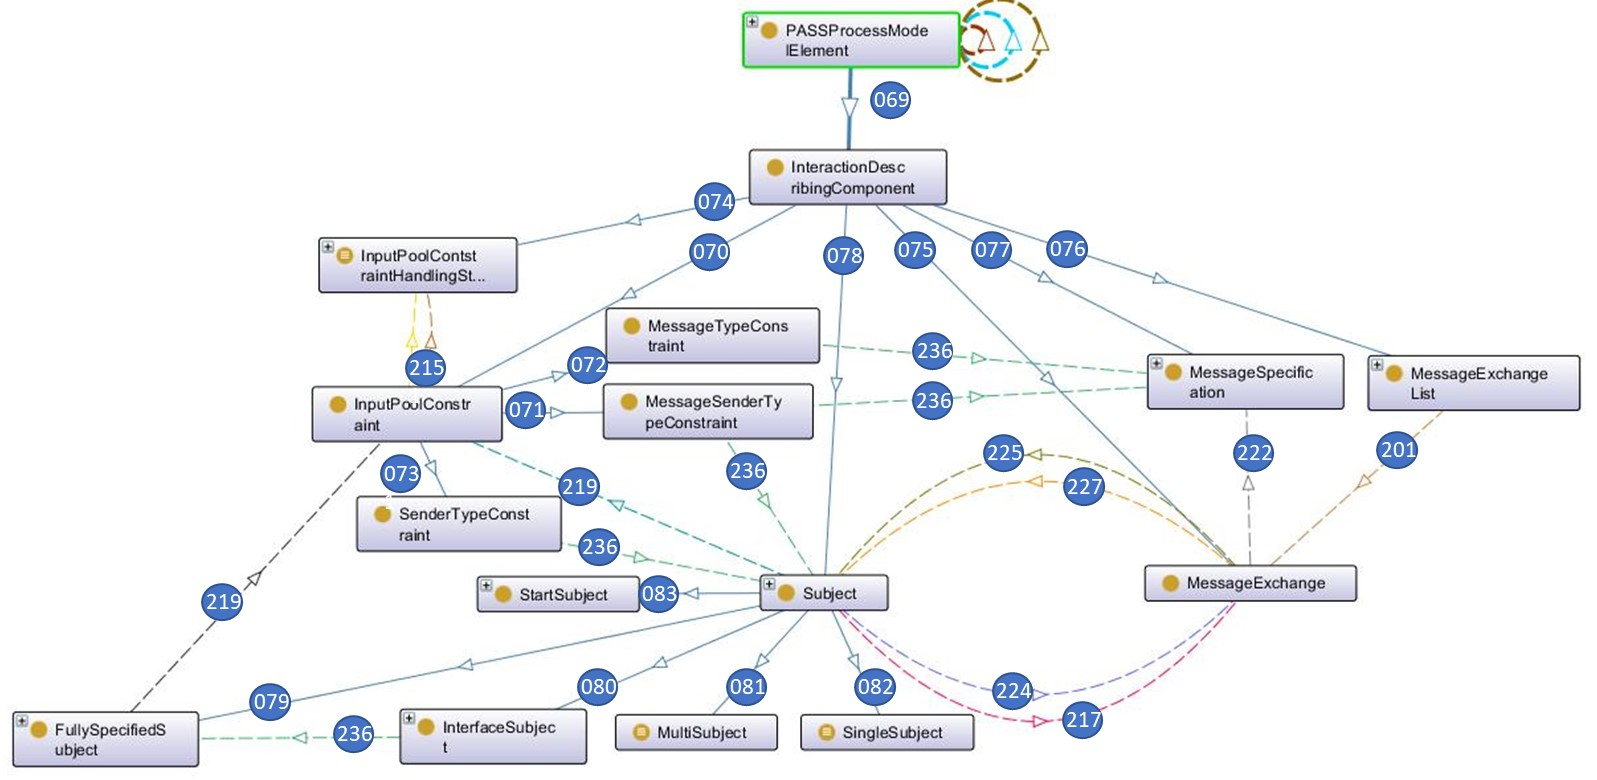
\includegraphics[width=1.0\linewidth]{Figures/Ontology/SubjectInteraction/OntoGrSubjectInteraction}
	\caption[Subject Interaction Diagram]{Subject Interaction Diagram}
	\label{fig:ontogrsubjectinteraction}
\end{figure*}

The central classes are \texttt{Subject} and \texttt{MessageExchange}. Between these classes are defined the properties \texttt{hasIncomingTransition} (in figure \ref{fig:ontogrsubjectinteraction} number 217) and \texttt{hasOutgoingTransition} (in figure \ref{fig:ontogrsubjectinteraction} number 224). These properties define that subjects have incoming and outgoing messages. Each message has a sender and a receiver (in figure \ref{fig:ontogrsubjectinteraction} number 227 and number 225). Messages have a type. This is expressed by the property \texttt{hasMessageType} (in figure \ref{fig:ontogrsubjectinteraction} number 222). Instead of the property 222 a message exchange may have the property 201 if a list of messages is used instead of a single message.

Each subject has an input pool. Input pools have three types of constraints (see section \ref{sec: inputpool}). This is expressed by the property references  (in figure \ref{fig:ontogrsubjectinteraction} number 236) and \texttt{InputPoolConstraints} (in figure \ref{fig:ontogrsubjectinteraction} number 219). Constraints which are related to certain messages have references to the class \texttt{MessageSpecification}.

There are four subclasses of the class \texttt{subject} (in figure \ref{fig:ontogrsubjectinteraction} number 079, 080, 081 and 082). The specialties of these subclasses are described in section \ref{sec: Subject}. A class \texttt{StartSubject} (in figure \ref{fig:ontogrsubjectinteraction} number 83) which is a subclass of class subject denotes the subject in which a process instance is started.

All other relations are subclass relations. The class \texttt{PASSProcessModelElement} is the central PASS class. From this class, all the other classes are derived (see next sections). From class \texttt{InteractionDescribingComponent} all the classes required for describing the structure of a process system are derived.

\section{ASM Description}

In this chapter, only the structure of a PASS model is considered. Execution has not been considered. Because ASM only considers execution aspects in this chapter an ASM specification of the structural aspects does not make sense. The execution semantics is part of chapter 4.

\chapter{Execution of a PASS Model}
\label{PASSExec}

\section{Subjects and Subject carrier}
\label{sec:subjectCarrier} 

\begin{figure*}[htbp]
	\centering
	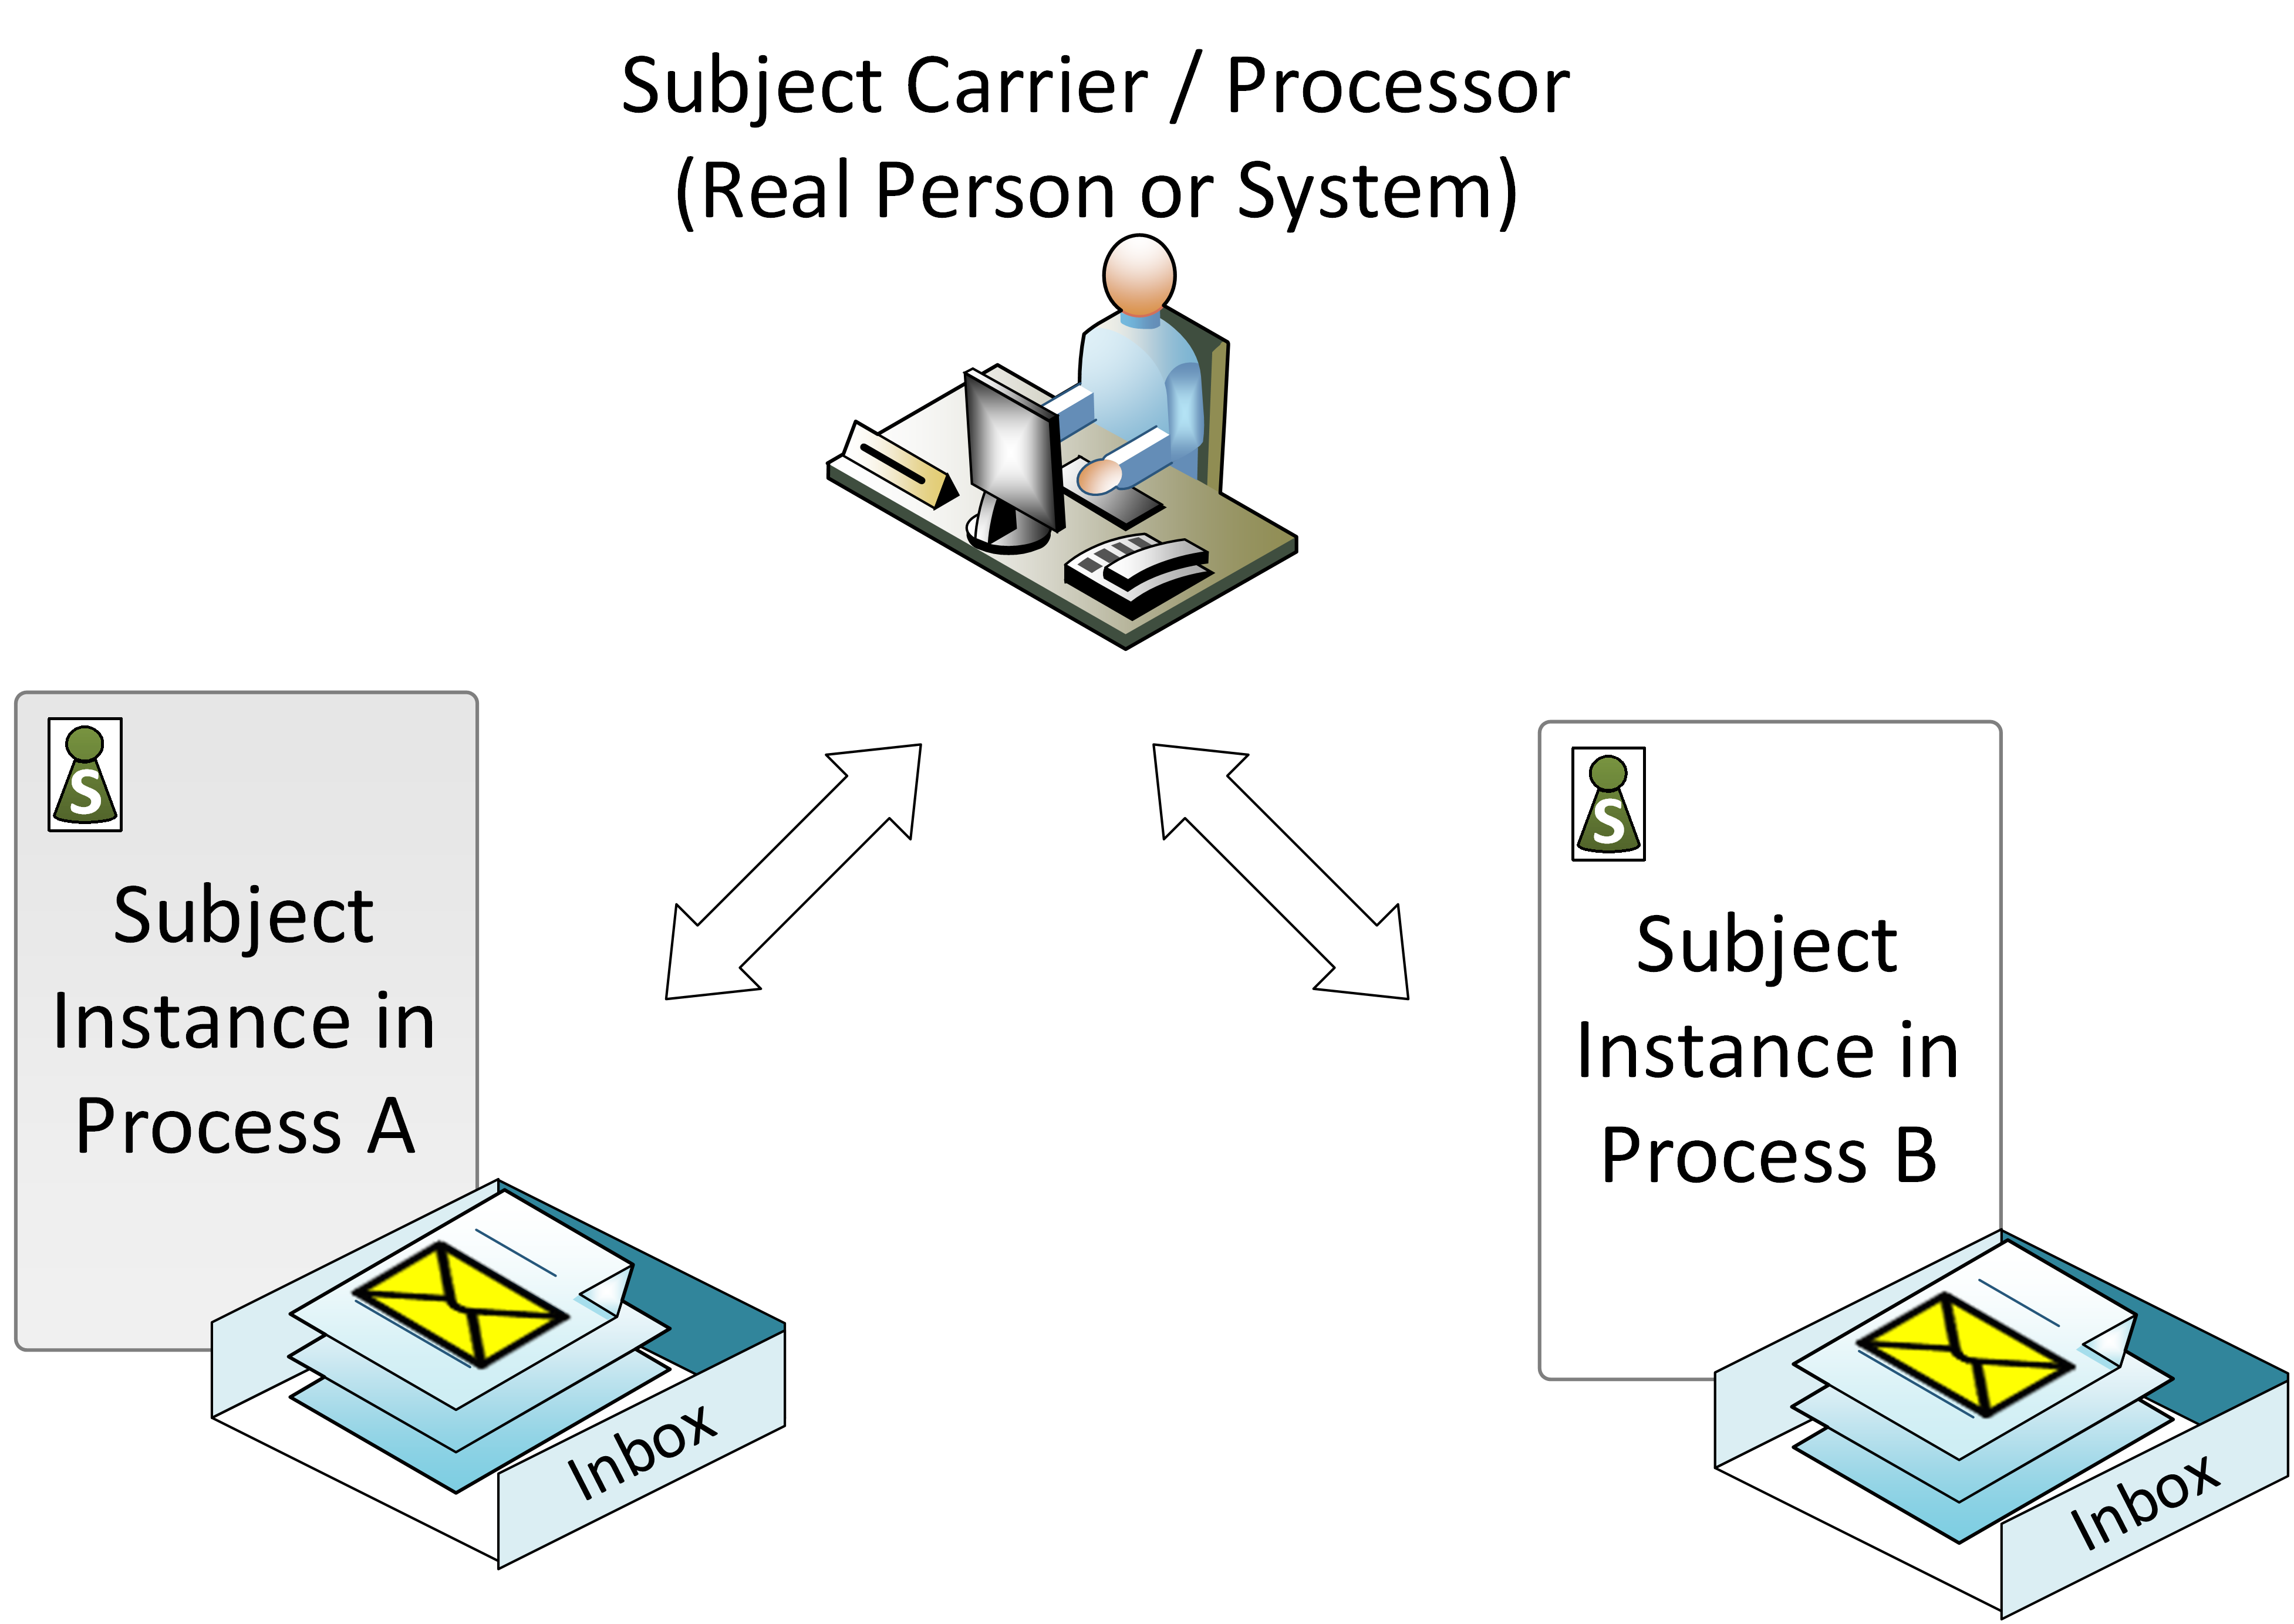
\includegraphics[width=0.5\linewidth]{Figures/SubjectCarrierConcept1.png}
	\caption[Concept of one Subject Carrier(processor) responsible for multiple Subjects in different process, each with its individual inbox (\cite{elstermann:diss})]{Concept of one Subject Carrier(processor) responsible for multiple Subjects in different process, each with its individual inbox(\cite{elstermann:diss})}
	\label{fig:subjectCarrierConcept1}
\end{figure*}

\begin{figure*}[htbp]
	\centering
	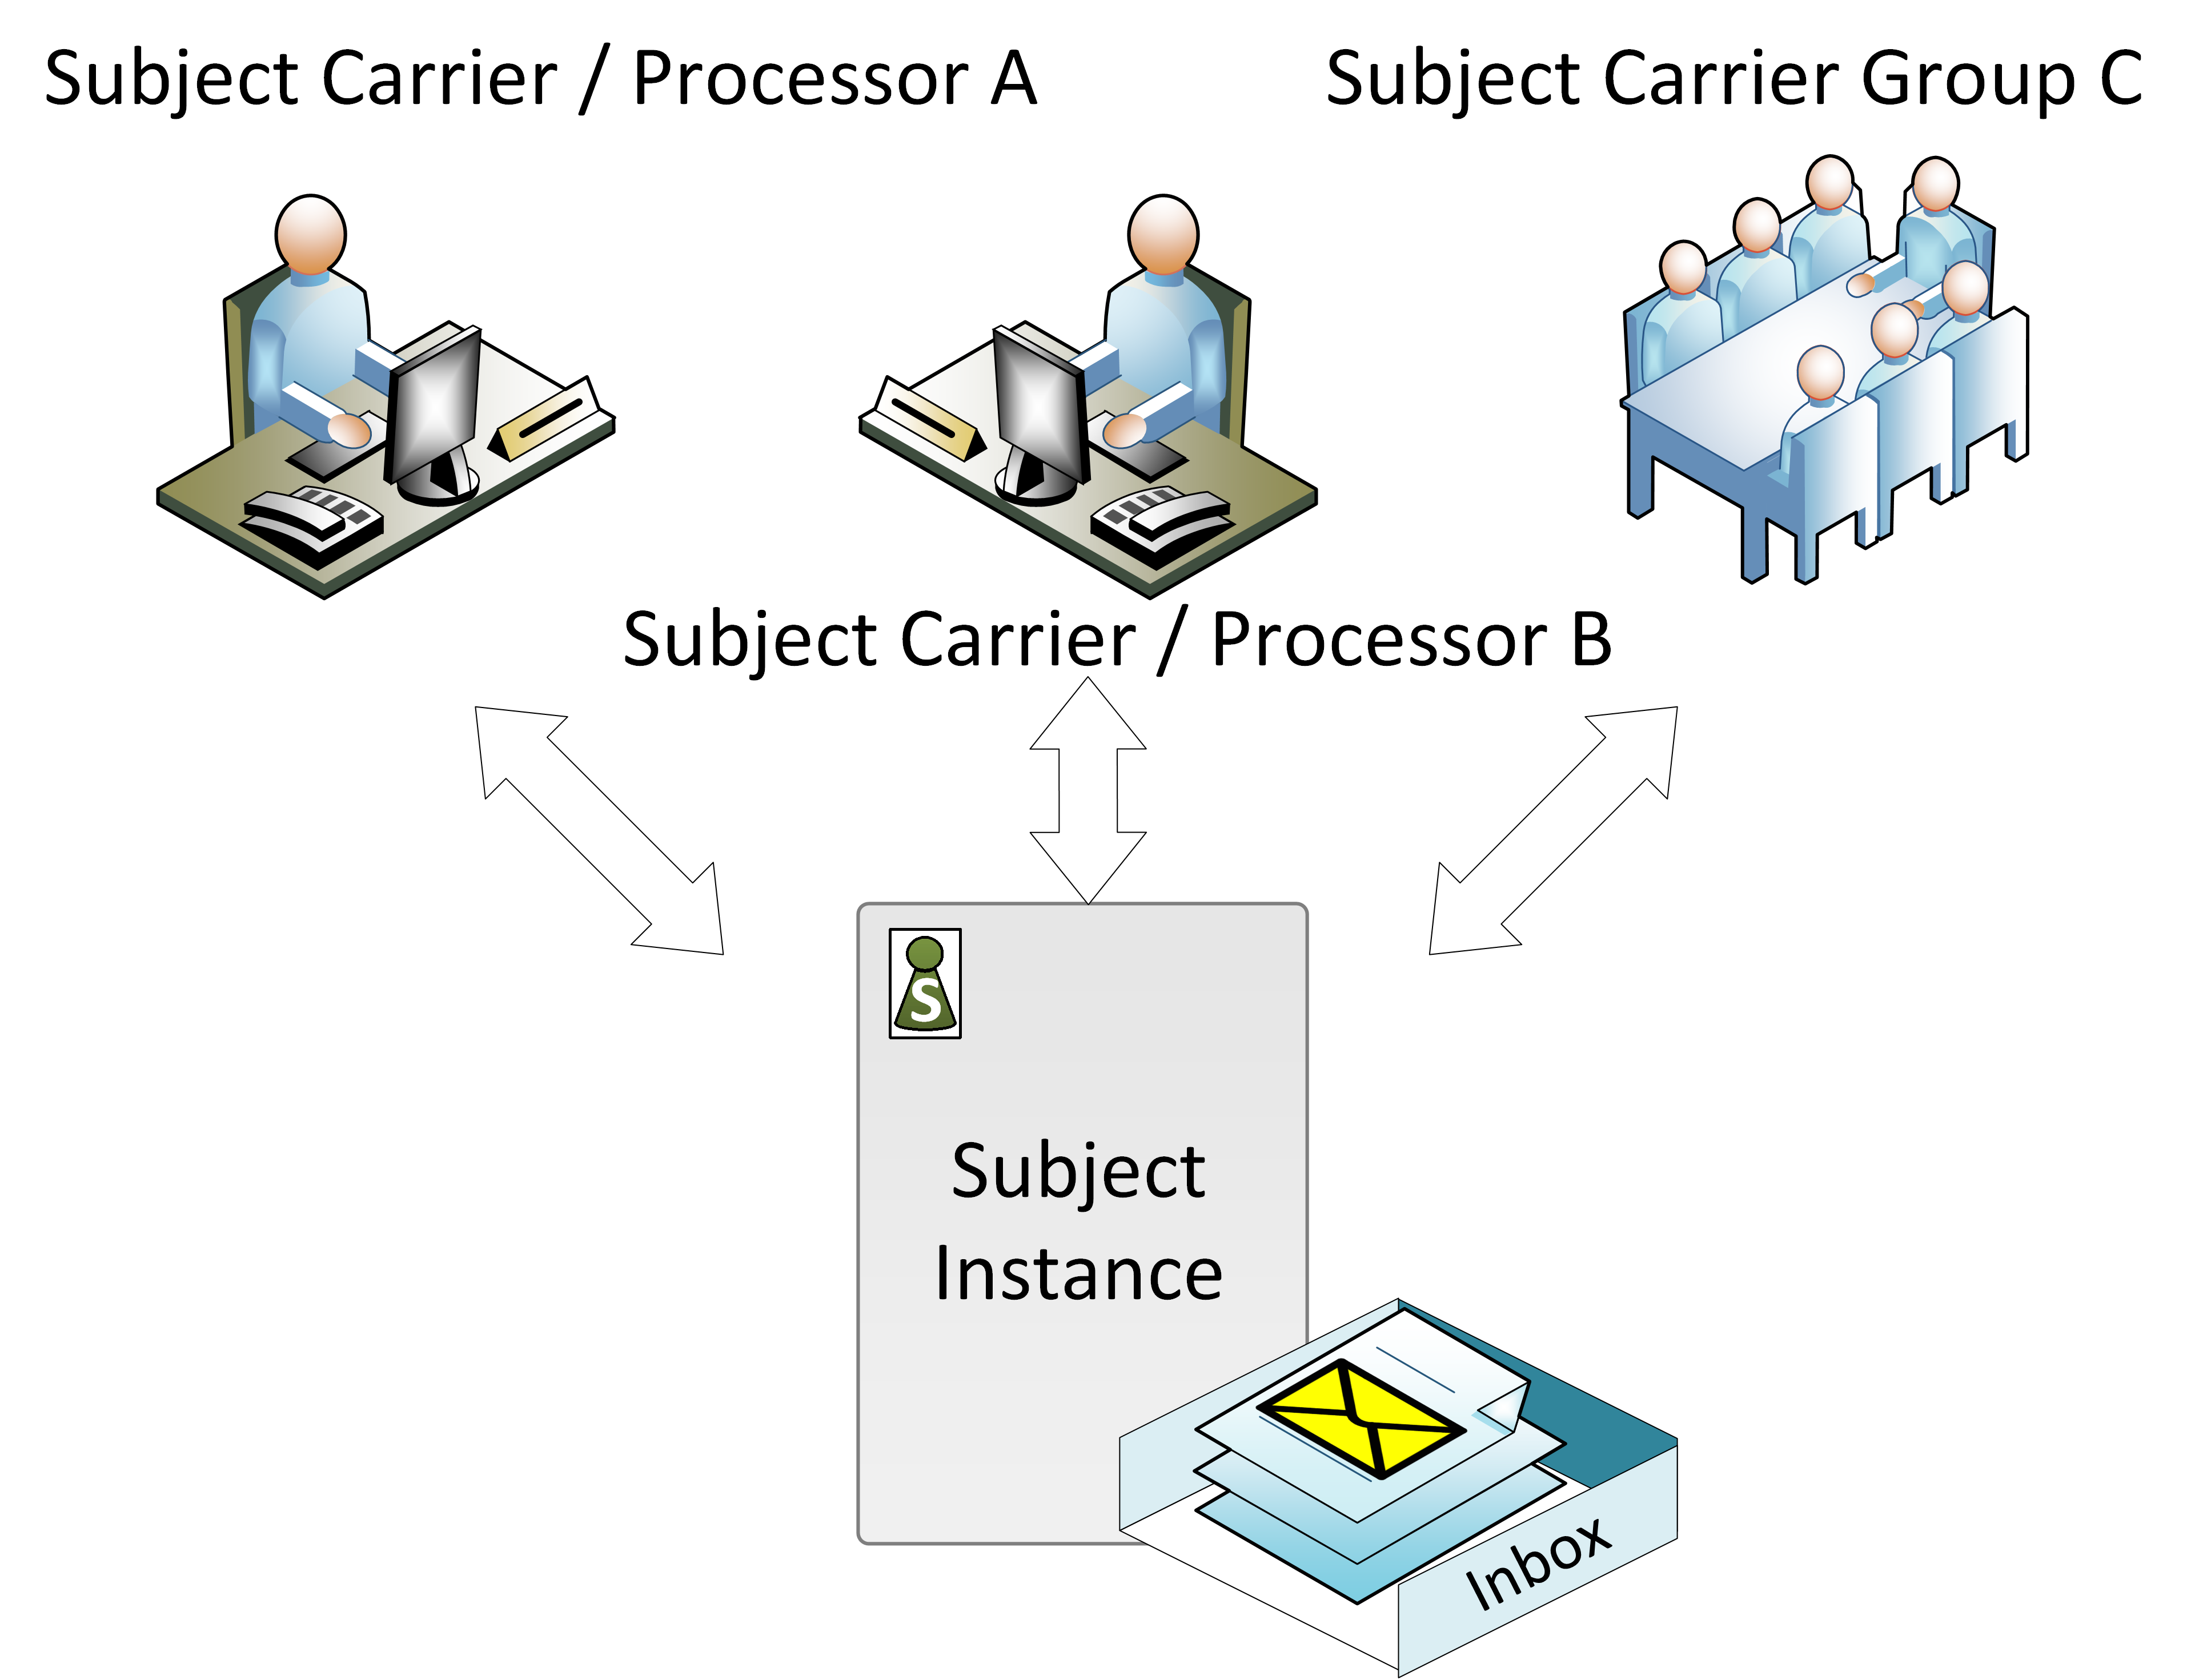
\includegraphics[width=0.5\linewidth]{Figures/SubjectCarrierConcept2.png}
	\caption[Concept of multipe Subject Carriers (processors) that can alternate in the the execution of on subject instance in a process (\cite{elstermann:diss})]{Concept of multipe Subject Carriers (processors) that can alternate in the the execution of on subject instance in a process (\cite{elstermann:diss})}
	\label{fig:subjectCarrierConcept2}
\end{figure*}

\subsection{Choice Segment Execution}
\label{sec:choiceSegmentExecution}

- Subjects can not be in more than one state at the same time
- It could be argued that the Choice Segment is somewhat contradicting this statement
- It is not
- simple interpretation: choice segment simply a short cut and better, more compact variant to modeling a multitude of possible paths as is shown in figure \ref{fig:choiceSegmentExecutionInterpretation}
- somewhat more complex execution concept: it is possible to alternate the execution of states (including their internal functions)

\begin{figure*}[htbp]
	\centering
	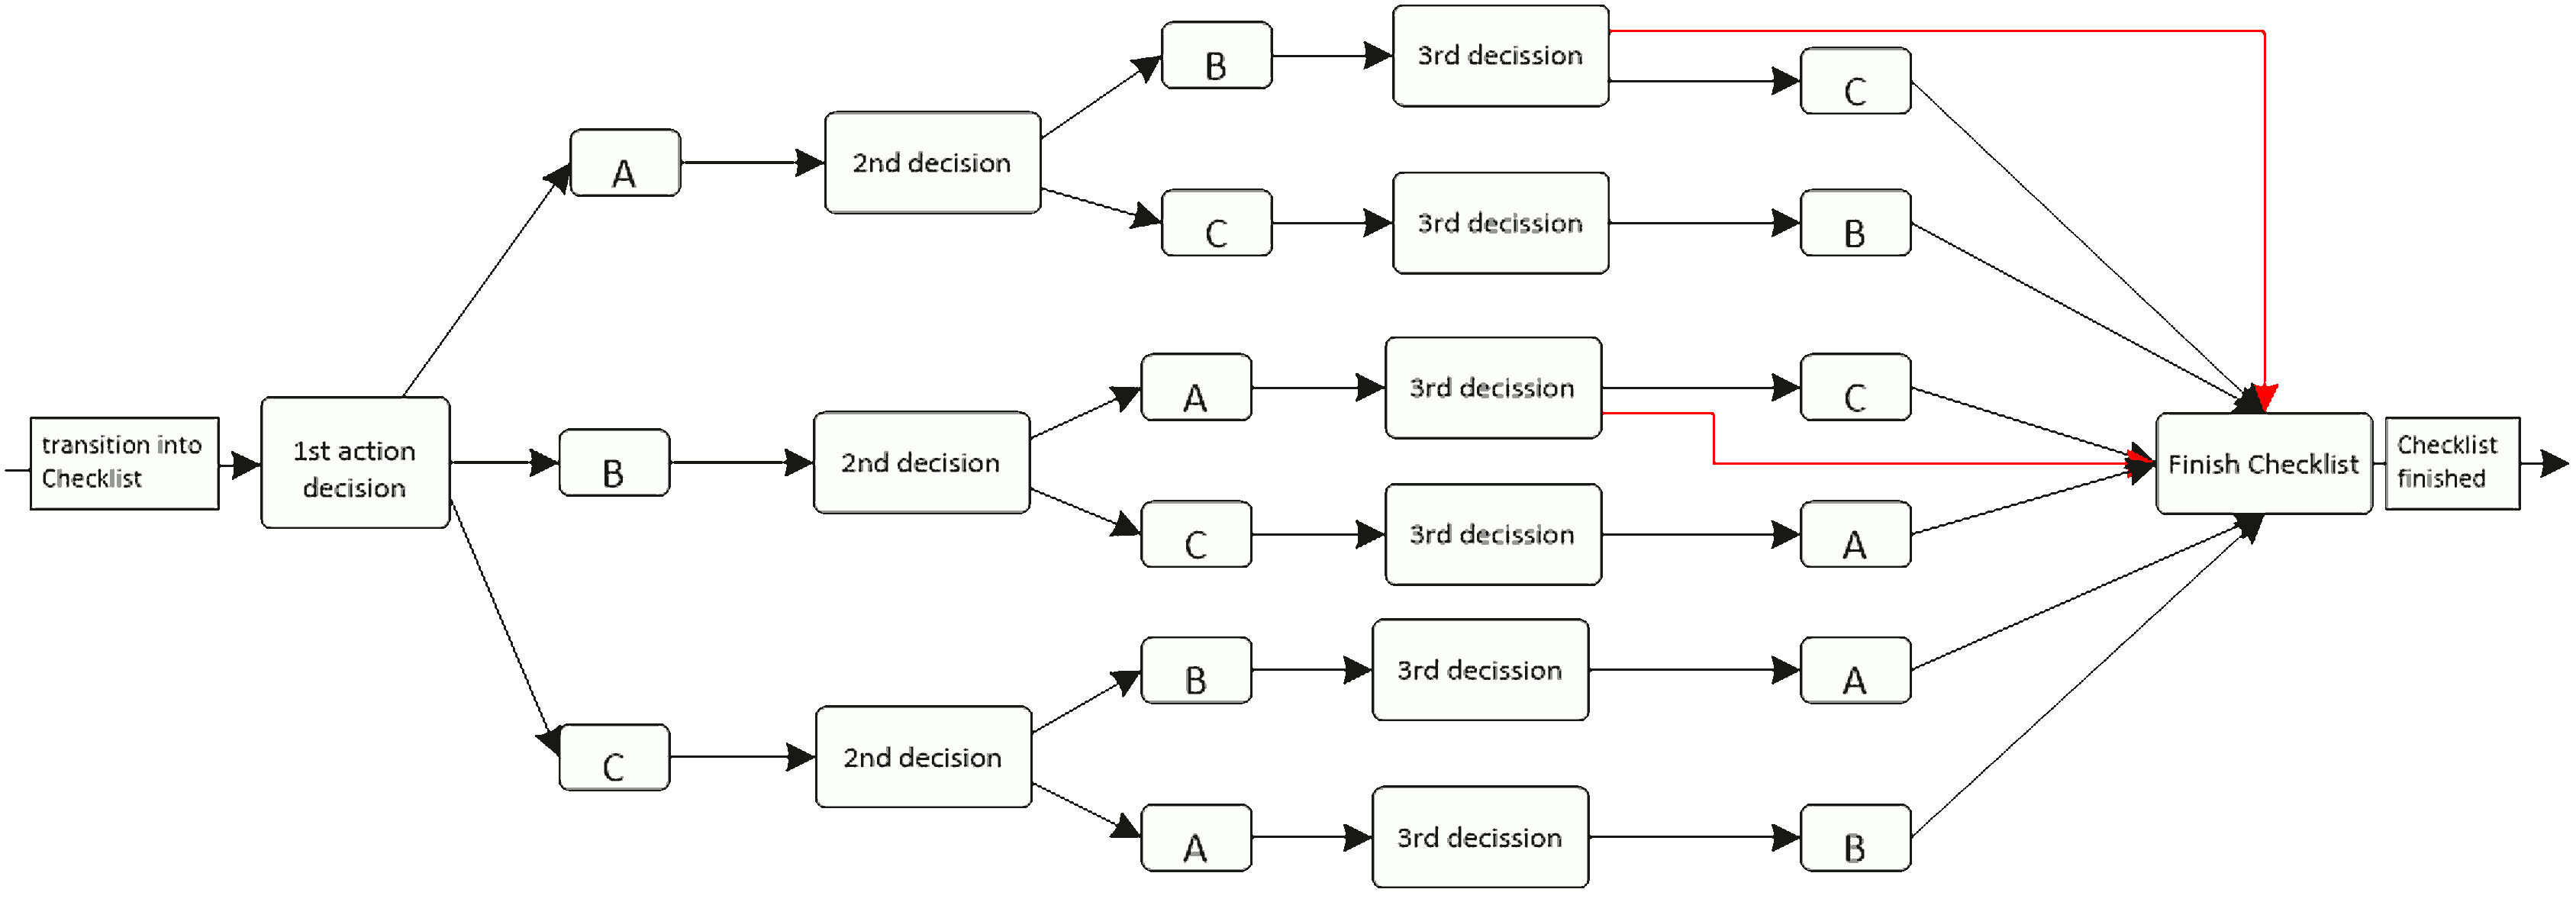
\includegraphics[width=0.5\linewidth]{Figures/Ontology/SubjectBehavior/ChoiceSegmentInterpretation.png}
	\caption[Execution Interpretation of a Choice Segment]{Execution Interpretation of a Choice Segment}
	\label{fig:choiceSegmentExecutionInterpretation}
\end{figure*}

The individual actions in the alternative paths of an alternative clause may be arbitrarily executed in parallel and overlapping (CS: interleving?), or in other words: A step can be executed in an alternative sequence, and then be followed by an action in any other sequence. This gives the performer of a subject the appropriate freedom of choice while executing his actions.

In the example, the order can thus first be updated, and then the message 'order arrived' sent to sales. Now, either the message 'deliver order' can be sent to the warehouse or one of the internal functions, 'update sales status' or 'collect data for statistics', can be executed.

The left alternative must be executed completely, and the middle alternative must also have been completed, if the first action ('inform sales' in the example) is executed. Only the left alternative can be processed because the middle one was never started. Alternatively, the sequence in the middle may have already reached its endpoint, while the left is not yet complete. In this case, the process waits until the left one has reached its endpoint. Only then will the state 'confirmation' be reached in the alternative clause. The right branch neither needs to be started, nor to be completed. It is therefore irrelevant for the completion of the alternative construct.

\section{Informal Description of Subject Behavior Execution}


%ME: for now i have put all descriptions of SBD model elements into chapter 2b
%all aspects concerning execution are to be re put into this chapter


Before sending a message, the values of the parameters to be transmitted need to be determined. In case the message parameters are simple data types, the required values are taken from local variables or business objects of the sending subject, respectively. In the case of business objects, a current instance of a business object is transferred as a message parameter.

The sending subject attempts to send the message to the target subject and store it in its input pool. Depending on the described configuration and status of the input pool, the message is either immediately stored or the sending subject is blocked until delivery of the message is possible.

%The blocking of subjects when attempting to send can be monitored over time with the so-called timeout. The example in Figure \ref{fig:sendstatetimer} shows with 'Timeout: 24 h' an additional state transition which occurs when within 24 hours one of the two messages cannot be sent. If a value of zero is specified for the timeout, the process immediately follows the timeout path when the alternative message delivery fails.

\subsection{Receiving Messages}

Analogously to sending, the receiving procedure is divided into two phases, which run inversely to send.

The first step is to verify whether the expected message is ready for being picked up. In the case of synchronous messaging, it is checked whether the sending subject offers the message. In the asynchronous version, it is checked whether the message has already been stored in the input pool. If the expected message is accessible in either form, it is accepted, and in a second step, the corresponding state transition is performed. This leads to a takeover of the message parameters of the accepted message to local variables or business objects of the receiving subject. In case the expected message is not ready, the receiving subject is blocked until the message arrives and can be accepted.

In a certain state, a subject can expect alternatively multiple messages. In this case, it is checked whether any of these messages are available and can be accepted. The test sequence is arbitrary unless message priorities are defined. In this case, an available message with the highest priority is accepted. However, all other messages remain available (e.g., in the input pool) and can be accepted in other receive states.

Figure \ref{fig:receivestate} shows a receive state of the subject 'employee' which is waiting for the answer regarding a business trip request. The answer may be an approval or a rejection.

\begin{figure*}[htbp]
	\centering
	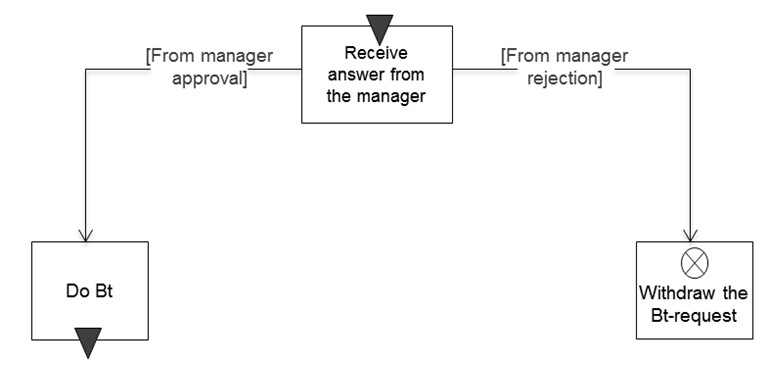
\includegraphics[width=0.7\linewidth]{Figures/Ontology/SubjectBehavior/ReceiveState}
	\caption[Example of alternative receiving]{Example of alternative receiving}
	\label{fig:receivestate}
\end{figure*}

Just as with sending messages, also receiving messages can be monitored over time. If none of the expected messages are available and the receiving subject is therefore blocked, a time limit can be specified for blocking. After the specified time has elapsed, the subject will execute the transition as it is defined for the timeout period. The duration of the time limit may also be dynamic, in the sense that at the end of a process instance the process stakeholders assigned to the subject decide that the appropriate transition should be performed. We then speak of a manual timeout.

\subsection{Sending Messages}




%\begin{figure}[htbp]
%	\centering
%	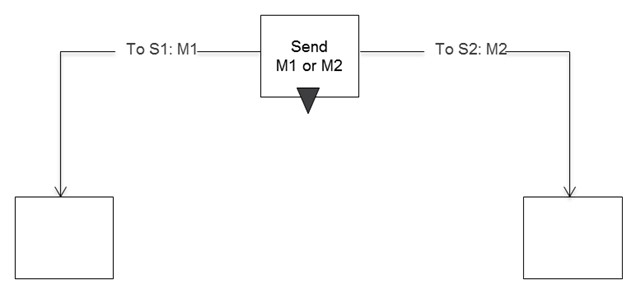
\includegraphics[width=0.7\linewidth]{Figures/Ontology/SubjectBehavior/sendState}
%	\caption[Example of alternative sending]{Example of alternative sending}
%	\label{fig:sendstate}
%\end{figure}

%By specifying priorities, the order of sending can be influenced. For example, it can be determined that the message M1 to S1 has a higher priority than the message M2 to S2. Using this specification, the sending subject starts with sending message M1 to S1 and then tries only in case of failure to send message M2 to S2. In case of message M2 can also not be sent to the subject S2, the attempts to send start from the beginning.

%The blocking of subjects when attempting to send can be monitored over time with the so-called timeout. The example in Figure \ref{fig:sendstatetimer} shows with 'Timeout: 24 h' an additional state transition which occurs when within 24 hours one of the two messages cannot be sent. If a value of zero is specified for the timeout, the process immediately follows the timeout path when the alternative message delivery fails.

%\begin{figure*}[htbp]
%	\centering
%	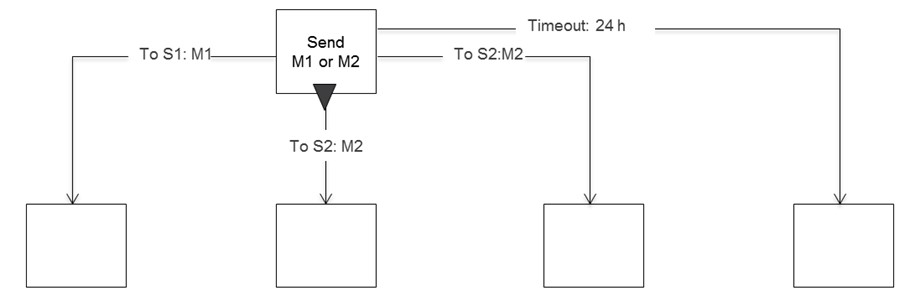
\includegraphics[width=0.7\linewidth]{Figures/Ontology/SubjectBehavior/SendSTateTimer}
%	\caption[Send using time monitoring]{Send using time monitoring}
%	\label{fig:sendstatetimer}
%\end{figure*}
% Review Christian Stary January 2020
\section{ASM Definition of Subject Execution}

\setminted{fontsize=\small}
\setmintedinline{fontsize=\normalsize,breaklines}

This section provides a commented overview of the CoreASM PASS Reference Implementation provided in Appendix~\ref{CoreASM-Reference-Implementation}.
Only a reduced set of language elements are shown here, advanced Functions and implementation details are left out,
which allowed it to shorten various rules for a focus on their core semantics.
Therefore all contents of this section are a non-normative introduction to the topic of formal execution semantics.

There are some conceptional differences between the reference implementation and the OWL description.
The End State is a distinguished state instead of a property of a Do State or Receive State.
Choice Segment Paths are always both mandatory to start and end, also they have to be started with the Modal Split Function and joined with the Modal Join Function.
Furthermore the reference implementation supports advanced features that are not covered by the OWL description, for example the Mobility of Channels concept and CorrelationIDs.
A complete comparision of the conceptual differences is given in~\ref{CoreASM-Reference-Implementation-Differences-OWL-Model}.

%simplifications for this chapter:
%- no Observer support => no execution state, no state priorities => Cancel Function not required
%- limited scope to InternalAction, Send, Receive, CallMacro, ModalSplit/ModalJoin, End to provide a closed set of features
%  => no VarMan, Cancel, SelectAgents, Tau
%- discuss: proper-termination and CloseIP/OpenIP are motivated from interaction soundness. include? mention? hard-exclude (remove references from code)?
%- no KillBehavior (although recursive macros and reservation messages). therefore this will not be sound - but a bit less complicated


\subsection{Architecture}

The reference implementation is composed by three main components.
The specification of the execution semantics is defined with Abstract State Machines (ASM) % TODO: ref Börger?
and written in the CoreASM dialect.
The specification is interpreted by the CoreASM Engine,
which is part of the open-source CoreASM Framework and written for the Java Virtual Machine. % TODO: ref?
The third component is a console application that is connected to the CoreASM Engine
and enables an interactive abstract process evaluation.
A detailed description of the architecture is given in~\ref{CoreASM-Reference-Implementation-Architecture}.


\subsection{Foundation}

The specification makes use of asynchronous multi-agent Turbo ASMs, executing each Subject instance with one ASM-agent each.
It supports the concurrent execution of multiple process models and multiple instances of each process model.
Each instance has a unique \textit{ProcessInstanceID} (short: \asminline{PI}) assigned.
Within a process instance multiple instances of a subject can occur (MultiSubject concept).
Each subject instance has an agent assigned, to distinguish the subject instances.
This agent is identified by it name.
Therefore a subject instance is identified by the tuple (Process~Model~ID, Process~Instance~ID, Subject~ID, Agent~Name).
This tuple is called \textit{Channel} (short: \asminline{ch}), as it used in the mobility of channels concept in order to support distributed communication patterns.

In the interpreter, each subject instance has an ASM Agent assigned, that keeps track of its current state,
where the meaning of state is in the sense of which subject data is present, the content of the input pool queues and also the active SBD states.
This state is stored in ASM functions and assigned to the \textit{Channel}.

\begin{listing}[htbp]
\begin{minted}{lexer.py:CoreASMLexer -x}
// ASM Agent -> Channel
function channelFor : Agents -> LIST

derived processIDFor(a)       = processIDOf(channelFor(a))
derived processInstanceFor(a) = processInstanceOf(channelFor(a))
derived subjectIDFor(a)       = subjectIDOf(channelFor(a))
derived agentFor(a)           = agentOf(channelFor(a))

derived processIDOf(ch)       = nth(ch, 1)
derived processInstanceOf(ch) = nth(ch, 2)
derived subjectIDOf(ch)       = nth(ch, 3)
derived agentOf(ch)           = nth(ch, 4)
\end{minted}
\caption{Channel definitions}
\label{lst:shortasm:channelFor}
\end{listing}

In the function \asminline{channelFor} the assignment from the ASM Agents to their \textit{Channels} is stored.
The derived functions are used to lookup certain tuple elements of the channel.\\

% NOTE: StartProcess and StartASMAgent left out intentionally

% Subject Data / Data Objects

Analogous to programming languages Data Objects are called \textit{Variables}.
Their scope is either bound to a Subject or a Macro Instance and can only be
accessed by the Subject. Variables are identified by their name and have an
explicit data type and a value.

Variables are stored in the \asminline{variable} function which maps from
the Subject's Channel, the scoped Macro Instance~ID and the Variable's name to
a pair of the data type and value. For Variables that are not scoped to a Macro
Instance, and are therefore accessible for any state in any Macro Instance of
the Subject, the unused Macro Instance~ID~0 is used.

The function \asminline{variableDefined} is used to keep track of Variables
that are in use, so that their content can be reset upon the termination of a
Macro Instance or the Subject, respectively.


\begin{listing}[htbp]
\begin{minted}{lexer.py:CoreASMLexer -x}
// Channel * macroInstanceNumber * varname -> [vartype, content]
function variable : LIST * NUMBER * STRING -> LIST

// Channel -> Set[(macroInstanceNumber, varname)]
function variableDefined : LIST -> SET
\end{minted}
\caption{variable}
\label{lst:shortasm:variable}
\end{listing}




\subsection{Interaction Definitions}\label{sec:InteractionDefinitions}

The interaction between Subjects is implemented as asynchronous Message exchange.
Messages are placed into the Inputpool of the receiver where they are then retrieved from when the receiver is in a Receive state.


\subsubsection{Messages}\label{sec:messages}

The message content consists of the actual payload and its data type. As the
reference implementation is intended only for an abstract process execution
the payload / business objects are abstracted to be just a text given as string.

For the communication with MultiSubjects, i.e. sending the same Message to
multiple Agents of one Subject, the \textit{all-or-none} strategy is used. This
is accomplished by separating the sending of a Message into two phases: first
a reservation Message is placed at each receiver into the input pool.
Only after all reservations could be placed they are then replaced with the
actual Message.

\subsubsection{Inputpool}\label{sec:Inputpool}

The Inputpool is structured into multiple FIFO queues per Subject~ID of the sender, the Messagetype and the CorrelationID.

The Inputpool can be limited to allow a maximum number of Messages and
reservations per sender Subject~ID and Messagetype; in case the Inputpool Limit is
reached no additional reservation can be placed. To support the proper
termination of a Subject a specific queue (and also the complete Inputpool)
can be closed, in which case no additional reservation can be placed into it,
too.

\begin{listing}[htbp]
\begin{minted}[escapeinside=~~]{lexer.py:CoreASMLexer -x}
// Channel * senderSubjID * msgType * correlationID
//   -> [msg1, msg2, ~\ldots~]
function inputPool : LIST * STRING * STRING * NUMBER -> LIST

/* stores all locations where an inputPool was defined */
// Channel -> {[senderSubjID, msgType, correlationID], ~\ldots~}
function inputPoolDefined : LIST -> SET

// Channel * senderSubjID * msgType * correlationID
function inputPoolClosed : LIST * STRING * STRING * NUMBER
  -> BOOLEAN
\end{minted}
\caption{inputPool}
\label{lst:shortasm:inputPool}
\end{listing}


The queues of the Inputpool are stored in the \asminline{inputPool} function.
The function \asminline{inputPoolDefined} is used to keep track of the
locations of the queues that are in use, so that their content can be checked
upon termination. The function \asminline{inputPoolClosed} is used to store
whether a queue is closed. The special location
\asminline{inputPoolClosed(ch, undef, undef, undef)} is used to
store whether the complete Inputpool is closed.

The function \asminline{derived availableMessages(receiverChannel, senderSubjectID, msgType, ipCorrelationID)} returns the
Messages from the location \asminline{inputPool(receiverChannel,
senderSubjectID, msgType, ipCorrelationID)} that can be received, i.e. that it
filters out reservations and reduces Messages from the same sender to only
the oldest one.

\subsection{Subject Behavior}

The Subject Behavior consists at least of one \textit{Main Macro}
and might have an arbitrary number of minor Macros, called \textit{Additional Macros}.

\begin{listing}[htbp]
\begin{minted}{lexer.py:CoreASMLexer -x}
rule SubjectBehavior =
  MacroBehavior(1)
\end{minted}
\caption{SubjectBehavior}
\label{lst:shortasm:SubjectBehavior}
\end{listing}

% Macro Behavior

% NOTE: extemely shortened: no execution state => no remainingStates


The \asminline{MacroBehavior} rule controls the evaluation of all active
states for the given Macro Instance~ID~\asminline{MI}.


\begin{listing}[htbp]
\begin{minted}{lexer.py:CoreASMLexer -x}
rule MacroBehavior(MI) =
  let ch = channelFor(self) in
  choose stateNumber in activeStates(ch, MI) do
    Behavior(MI, stateNumber)
\end{minted}
\caption{MacroBehavior}
\label{lst:shortasm:MacroBehavior}
\end{listing}

From that list a state \asminline{stateNumber} is chosen to be evaluated with the \asminline{Behavior} rule.

% State


The evaluation of a state is structured into three main phases: initialization,
the state function and an optional transition behavior.

The state function is responsible for the selection of an outgoing transition and
has to supervise the Timeout. It also has to enable and disable its outgoing
transitions, meaning that transitions can be available depending on some dynamic state,
for example whether a certain Message is present in the Inputpool.
Usually the outgoing transition will be selected by the environment, however with
auto-transitions it is possible that such an transition is automatically selected as soon
as it becomes enabled and as long as there are no other transitions to select from.


\begin{listing}[htbp]
\begin{minted}{lexer.py:CoreASMLexer -x}
rule Behavior(MI, currentStateNumber) =
 let s = currentStateNumber,
    ch = channelFor(self) in
  if (initializedState(ch, MI, s) != true) then
    StartState(MI, s)
  else if (abortState(MI, s) = true) then
    AbortState(MI, s)
  else if (completed(ch, MI, s) != true) then
    Perform(MI, s)
  else if (initializedSelectedTransition(ch, MI, s) != true) then
    StartSelectedTransition(MI, s)
  else
   let t = selectedTransition(ch, MI, s) in
    if (transitionCompleted(ch, MI, t) != true) then
      PerformTransition(MI, s, t)
    else
      Proceed(MI, s, targetStateNumber(processIDFor(self), t))
\end{minted}
\caption{Behavior}
\label{lst:shortasm:Behavior}
\end{listing}


In the beginning the \asminline{Behavior} rule initializes the state with the
\asminline{StartState} rule, which will set \asminline{initializedState} to
\asminline{true}. If the function should not be aborted the \asminline{Perform}
rule calls the state behavior of the underlying function until it is
\asminline{completed}.
In the next phase the selected transition will be initialized by the
\asminline{StartSelectedTransition} rule and the transition behavior will be performed with
the \asminline{PerformTransition} rule until it is completed as well. As last step
the \asminline{Proceed} rule removes the current state and adds the selected
transition's target state.

%---

The environment has full read access to all functions of this semantics and knows
therefore each running Subject, their Macro Instances and their active states.

To define a homogeneous interface between the Function semantics and the environment we
define the function \asminline{wantInput} to be written by an Function when it
requires an external input, for example if an outgoing transition has to be chosen.



\begin{listing}[htbp]
\begin{minted}{lexer.py:CoreASMLexer -x}
// Channel * MacroInstanceNumber * StateNumber -> Set[String]
function wantInput : LIST * NUMBER * NUMBER -> SET
\end{minted}
\caption{wantInput}
\label{lst:shortasm:wantInput}
\end{listing}


This function is read by our console application for all active states
to present the user a list of possible decisions that can be made.

The environment then writes its external input in a corresponding function, for
example for a transition decision into the \asminline{selectedTransition} function, and
clears the \asminline{wantInput} function of that state.

The \asminline{SelectTransition} rule adds the \asminline{"TransitionDecision"}
requirement into the \asminline{wantInput} function.


\begin{listing}[htbp]
\begin{minted}{lexer.py:CoreASMLexer -x}
rule SelectTransition(MI, currentStateNumber) =
  let ch = channelFor(self),
       s = currentStateNumber in
  if (|outgoingEnabledTransitions(ch, MI, s)| = 0) then
    skip // BLOCKED: none to select
  else if (not(contains(wantInput(ch, MI, s),
                        "TransitionDecision"))) then
    add "TransitionDecision" to wantInput(ch, MI, s)
  else
    skip // waiting for selectedTransition
\end{minted}
\caption{SelectTransition}
\label{lst:shortasm:SelectTransition}
\end{listing}


If the \asminline{wantInput} function already contains the
\asminline{"TransitionDecision"} requirement nothing needs to be done and another
state can be evaluated by the \asminline{MacroBehavior} rule.
The same applies if there are no outgoing transitions enabled.
Otherwise the requirement is added to the \asminline{wantInput} function.


\subsection{Internal Action}


The \emph{Internal Action} is used to model DoStates, Subject-internal activities and decisions.
It is labeled with a textual description of the activity that the Agent should perform.
The outgoing transitions are labeled with a textual description of the possible execution results.
Since the activity is performed outside of the interpreter all outgoing transitions are enabled from the beginning on and no transition rule has to be defined.
Therefore the state function only consists of the timeout check and transition selection.


\begin{listing}[htbp]
\begin{minted}{lexer.py:CoreASMLexer -x}
rule StartInternalAction(MI, currentStateNumber) = {
  StartTimeout(MI, currentStateNumber)

  EnableAllTransitions(MI, currentStateNumber)
}
\end{minted}
\caption{StartInternalAction}
\label{lst:shortasm:StartInternalAction}
\end{listing}



The initialization of the InternalAction starts the Timeout and enables all
outgoing transitions.


\begin{listing}[htbp]
\begin{minted}{lexer.py:CoreASMLexer -x}
rule PerformInternalAction(MI, currentStateNumber) =
  let ch = channelFor(self),
       s = currentStateNumber in
    if (shouldTimeout(ch, MI, s) = true) then {
      SetCompleted(MI, s)
      ActivateTimeout(MI, s)
    }
    else if (selectedTransition(ch, MI, s) != undef) then
      SetCompleted(MI, s)
    else
      SelectTransition(MI, s)
\end{minted}
\caption{PerformInternalAction}
\label{lst:shortasm:PerformInternalAction}
\end{listing}


The state function checks if a Timeout should be activated; otherwise the
\asminline{SelectTransition} rule is called until the \asminline{selectedTransition} function has
been set.




\subsection{Send Function}


The Send Function sends a Message. Disregarding the optional Timeout and Cancel
transitions it must have exactly one outgoing transition which has to have parameters that
define at least the Messagetype and the receiver's Subject~ID.

An \textit{all-or-none} strategy is used to send Messages to MultiSubjects,
which means that the actual Message is only send when all receivers are able
to store it in their Inputpool. Therefore the Send Function is structured into
two phases: in the first phase, realized as state function, reservation Messages
are placed and in the second phase, realized as transition function, these reservations
are replaced with the actual Message.

To place a reservation in a receiver's Inputpool there must be space available
in the corresponding queue and the receiver must not be
\textit{non-proper} terminated.


\begin{listing}[htbp]
\begin{minted}{lexer.py:CoreASMLexer -x}
// Channel * MacroInstanceNumber * StateNumber -> Set[Messages]
function receivedMessages : LIST * NUMBER * NUMBER -> SET

// Channel * MacroInstanceNumber * StateNumber -> Set[Channel]
function receivers : LIST * NUMBER * NUMBER -> SET

// Channel * MacroInstanceNumber * StateNumber
function messageContent       : LIST * NUMBER * NUMBER -> LIST
function messageCorrelationID : LIST * NUMBER * NUMBER -> NUMBER
function messageReceiverCorrelationID : LIST * NUMBER * NUMBER
  -> NUMBER

// Channel * MacroInstanceNumber * StateNumber -> Set[Channel]
function reservationsDone : LIST * NUMBER * NUMBER -> SET

function nextCorrelationID : -> NUMBER
function nextCorrelationIDUsedBy : NUMBER -> Agents
\end{minted}
\caption{receivedMessages}
\label{lst:shortasm:receivedMessages}
\end{listing}


The Send Function stores the message content it has to send in the
\asminline{messageContent} function. The \asminline{receivers} function is
used to store the required receivers. When a reservation message has been
placed at a receiver its Channel is added to the \asminline{reservationsDone}
function.

The global function \asminline{nextCorrelationID} is used to increment
CorrelationIDs. To ensure the uniqueness of a CorrelationID the
\asminline{nextCorrelationIDUsedBy} function is used to store the ASM agent
that used the given CorrelationIDs.


\begin{listing}[htbp]
\begin{minted}{lexer.py:CoreASMLexer -x}
rule StartSend(MI, currentStateNumber) =
  let ch = channelFor(self),
     pID = processIDFor(self),
       s = currentStateNumber in
  // there must be exactly one transition
  let  t = first_outgoingNormalTransition(pID, s) in {
    receivers(ch, MI, s) := undef
    reservationsDone(ch, MI, s) := {}
    let mcVName = messageContentVar(pID, t) in
      messageContent(ch, MI, s) := loadVar(MI, mcVName)

    // generate new CorrelationID now, it will be stored
    // in a Variable once the message(s) are send
    let cIDVName = messageNewCorrelationVar(pID, t) in
      if (cIDVName != undef and cIDVName != "") then {
        messageCorrelationID(ch, MI, s) := nextCorrelationID
        nextCorrelationID := nextCorrelationID + 1
        // ensure no other agent uses this same correlationID
        nextCorrelationIDUsedBy(nextCorrelationID) := self
      }
      else
        messageCorrelationID(ch, MI, s) := 0

    // load receiver IP CorrelationID now, to avoid
    // influences of any changes of that variable
    let cIDVName = messageWithCorrelationVar(pID, t) in
    let cID = loadCorrelationID(MI, cIDVName) in
      messageReceiverCorrelationID(ch, MI, s) := cID
  }
\end{minted}
\caption{StartSend}
\label{lst:shortasm:StartSend}
\end{listing}


The initialization of the Send Function resets / initializes the \asminline{receivers} and
\asminline{reservationsDone} functions.
If the communication transition has a \asminline{messageContentVar} parameter given the
content of that Variable is loaded and stored in the \asminline{messageContent}
function. If it has a \asminline{messageNewCorrelationVar} parameter given
a new CorrelationID is created and stored in the \asminline{messageCorrelationID} function.
It will be stored in the Variable after the messages have been send.
If the message that will be send correlates to a previous message from the receiver
the CorrelationID from the Variable in \asminline{messageWithCorrelationVar} will be loaded
so that the message is stored in the corresponding input pool queue of the receiver.


\begin{listing}[htbp]
\begin{minted}{lexer.py:CoreASMLexer -x}
rule PerformSend(MI, currentStateNumber) =
  let ch = channelFor(self),
       s = currentStateNumber in
  if (receivers(ch, MI, s) = undef) then
    SelectReceivers(MI, s)
  else if (messageContent(ch, MI, s) = undef) then
    SetMessageContent(MI, s)
  else if (startTime(ch, MI, s) = undef) then
    StartTimeout(MI, s)
  else if (|receivers(ch, MI, s)| =
           |reservationsDone(ch, MI, s)|) then
    TryCompletePerformSend(MI, s)
  else if (shouldTimeout(ch, MI, s) = true) then {
    SetCompleted(MI, s)
    ActivateTimeout(MI, s)
  }
  else
    DoReservations(MI, s)
\end{minted}
\caption{PerformSend}
\label{lst:shortasm:PerformSend}
\end{listing}


In the state function the \asminline{SelectReceivers} rule is called until
the \asminline{receivers} have been selected. The \asminline{SelectReceivers} rule
interacts with the environment through the Selection and SelectAgent Functions
in order to either select existing Channels from a Variable, given as parameter
on the communication edge, or to select new assignments of Agents for the receiver
Subject.

The Timeout is started only when the \asminline{receivers} and the
\asminline{messageContent} functions are defined. Until all reservations are
placed, and if no Timeout occurs, the \asminline{DoReservations} rule attempts
to place further reservation messages. If all reservations are placed the
\asminline{TryCompletePerformSend} rule completes the state function, depending
on whether no receiver is \textit{non-proper} terminated.


\begin{listing}[htbp]
\begin{minted}{lexer.py:CoreASMLexer -x}
rule SetMessageContent(MI, currentStateNumber) =
  let ch = channelFor(self),
       s = currentStateNumber in
    if not(contains(wantInput(ch, MI, ch),
                    "MessageContentDecision")) then
      add "MessageContentDecision" to wantInput(ch, MI, ch)
    else
      skip // waiting for messageContent
\end{minted}
\caption{SetMessageContent}
\label{lst:shortasm:SetMessageContent}
\end{listing}



The \asminline{SetMessageContent} rule is called if no message content is
given as parameter on the communication transition until the \asminline{messageContent}
function is written by the environment.





\begin{listing}[htbp]
\begin{minted}{lexer.py:CoreASMLexer -x}
// handle all receivers
rule DoReservations(MI, currentStateNumber) =
  let ch = channelFor(self),
       s = currentStateNumber in
  let receiversTodo = (receivers(ch, MI, s) diff
                       reservationsDone(ch, MI, s)) in
  foreach receiver in receiversTodo do
    DoReservation(MI, s, receiver)
\end{minted}
\caption{DoReservations}
\label{lst:shortasm:DoReservations}
\end{listing}



The \asminline{DoReservations} rule iterates over all receivers that did not
already receive a reservation message. The \asminline{DoReservation} rule
then tries to place a reservation message for such receiver.

\begin{listing}[htbp]
\begin{minted}{lexer.py:CoreASMLexer -x}
// handle single reservation
// result true if hasPlacedReservation, adds to reservationsDone
rule DoReservation(MI, currentStateNumber, receiverChannel) =
  if (properTerminated(receiverChannel) = true) then
    let ch = channelFor(self),
       pID = processIDFor(self),
       sID = subjectIDFor(self),
         s = currentStateNumber in
    let Rch = receiverChannel,
       RpID = processIDOf(receiverChannel) in
    let sIDX = searchSenderSubjectID(pID, sID, RpID) in
    let msgCID = messageCorrelationID(ch, MI, s),
        RCID   = messageReceiverCorrelationID(ch, MI, s) in
    // there must be exactly one transition
    let t  = first_outgoingNormalTransition(pID, s) in
    let mT = messageType(pID, t) in
    let resMsg = [ch, mT, {}, msgCID, true] in
      seq
        // prepare receiver IP
        if (inputPool(Rch, sIDX, mT, RCID) = undef) then {
          add [sIDX, mT, RCID] to inputPoolDefined(Rch)
          inputPool(Rch, sIDX, mT, RCID) := []
        }
      next
        if (inputPoolIsClosed(Rch, sIDX, mT, RCID) != true) then
          if (inputPoolGetFreeSpace(Rch, sIDX, mT) > 0) then {
            enqueue resMsg into inputPool(Rch, sIDX, mT, RCID)
            add Rch to reservationsDone(ch, MI, s)
          }
          else
            skip // BLOCKED: no free space!
        else
          skip // BLOCKED: inputPoolIsClosed
  else
    skip // BLOCKED: non-properTerminated
\end{minted}
\caption{DoReservation}
\label{lst:shortasm:DoReservation}
\end{listing}


The \asminline{DoReservation} rule does not try to place a reservation message
if the receiver is \textit{non-proper} terminated. Otherwise it determines
the necessary parameters of the queue to use and builds the reservation message.
To support sending to an External Subject a translation of the sender's original
Subject~ID to the Subject~ID used in the External Process is performed by the
\asminline{searchSenderSubjectID} function.

When the queue at \asminline{inputPool(rCh, xSID, msgType, dstCorr)} was not
created yet a new queue is assigned to that location and remembered in the
\asminline{inputPoolDefined} function on the receiver's side.
If the queue is either closed or full no reservation message can be placed,
otherwise it is enqueued at the end.



\begin{listing}[htbp]
\begin{minted}{lexer.py:CoreASMLexer -x}
rule TryCompletePerformSend(MI, currentStateNumber) =
  let ch = channelFor(self),
     pID = processIDFor(self),
       s = currentStateNumber in
  if (anyNonProperTerminated(receivers(ch, MI, s)) = true) then
    if (shouldTimeout(ch, MI, s) = true) then {
      SetCompleted(MI, s)
      ActivateTimeout(MI, s)
    }
    else
      // BLOCKED: a receiver where a reservation was placed has
      // terminated non-proper in the meantime
      skip
  else {
    // there must be exactly one transition
    let t = first_outgoingNormalTransition(pID, s) in
      selectedTransition(ch, MI, s) := t

    SetCompleted(MI, s)
  }
\end{minted}
\caption{TryCompletePerformSend}
\label{lst:shortasm:TryCompletePerformSend}
\end{listing}


After all reservations could be placed the \asminline{TryCompletePerformSend}
rule has to ensure that no receiver terminated \textit{non-proper} in the
meantime. In that case the Send Function blocks and can only be left by a
Timeout or Cancel transition. Otherwise the state function is completed and the behavior can
continue with the transition function.


\begin{listing}[htbp]
\begin{minted}{lexer.py:CoreASMLexer -x}
rule PerformTransitionSend(MI, currentStateNumber, t) =
  let ch = channelFor(self),
     pID = processIDFor(self),
       s = currentStateNumber in {
    foreach r in reservationsDone(ch, MI, s) do {
      ReplaceReservation(MI, s, r)

      EnsureRunning(r)
    }

    let storeVName = messageStoreReceiverVar(pID, t) in
      if (storeVName != undef and storeVName != "") then
        SetVar(MI, storeVName, "ChannelInformation",
               reservationsDone(ch, MI, s))

    let cIDVName = messageNewCorrelationVar(pID, t) in
      if (cIDVName != undef and cIDVName != "") then
        SetVar(MI, cIDVName, "CorrelationID",
               messageCorrelationID(ch, MI, s))

    SetCompletedTransition(MI, s, t)
  }
\end{minted}
\caption{PerformTransitionSend}
\label{lst:shortasm:PerformTransitionSend}
\end{listing}


The transition function calls the \asminline{ReplaceReservation} rule to replace all
reservations with the actual Message. The \asminline{EnsureRunning} rule
(re)starts a receiver if it is not already running.
If the communication transition has the parameter \asminline{messageStoreReceiverVar} defined
the used receivers of the Message are stored in that Variable.
Also, if the communication transition has the parameter \asminline{messageNewCorrelationVar} defined
the CorrelationID that was created in \asminline{StartSend} and used for the send messages will be stored in the given Variable.


\begin{listing}[htbp]
\begin{minted}{lexer.py:CoreASMLexer -x}
rule ReplaceReservation(MI, currentStateNumber, receiverChannel) =
  let ch = channelFor(self),
     pID = processIDFor(self),
     sID = subjectIDFor(self),
       s = currentStateNumber in
  let Rch  = receiverChannel,
      RpID = processIDOf(receiverChannel) in
  let t  = first_outgoingNormalTransition(pID, s) in
  let mT = messageType(pID, t) in
  let sIDX   = searchSenderSubjectID(pID, sID, RpID),
      msgCID = messageCorrelationID(ch, MI, s),
      RCID   = messageReceiverCorrelationID(ch, MI, s) in
  let resMsg = [ch, mT, {}, msgCID, true],
      msg    = [ch, mT, messageContent(ch, MI, s), msgCID, false],
      IPold = inputPool(Rch, sIDX, mT, RCID) in
  let IPnew = setnth(IPold, head(indexes(IPold, resMsg)), msg) in
      inputPool(Rch, sIDX, mT, RCID) := IPnew
\end{minted}
\caption{ReplaceReservation}
\label{lst:shortasm:ReplaceReservation}
\end{listing}


Analogous to the \asminline{DoReservation} rule the
\asminline{ReplaceReservation} rule has to determine the queue and build both
the reservation message and the actual Message. It then can replace the reservation
in the queue with the actual message.


\begin{listing}[htbp]
\begin{minted}{lexer.py:CoreASMLexer -x}
rule AbortSend(MI, currentStateNumber) =
  let ch = channelFor(self),
       s = currentStateNumber in {
    foreach r in reservationsDone(ch, MI, s) do
      CancelReservation(MI, s, r)

    SetAbortionCompleted(MI, s)
  }
\end{minted}
\caption{AbortSend}
\label{lst:shortasm:AbortSend}
\end{listing}


To abort the Send Function all placed reservations have to be removed.


\begin{listing}[htbp]
\begin{minted}{lexer.py:CoreASMLexer -x}
rule CancelReservation(MI, currentStateNumber, receiverChannel) =
  let ch = channelFor(self),
     pID = processIDFor(self),
     sID = subjectIDFor(self),
       s = currentStateNumber in
  let Rch  = receiverChannel,
      RpID = processIDOf(receiverChannel) in
  let t  = first_outgoingNormalTransition(pID, s) in
  let mT = messageType(pID, t) in
  let sIDX   = searchSenderSubjectID(pID, sID, RpID),
      msgCID = messageCorrelationID(ch, MI, s),
      RCID   = messageReceiverCorrelationID(ch, MI, s) in
  let resMsg = [ch, mT, {}, msgCID, true],
      IPold = inputPool(Rch, sIDX, mT, RCID) in
  let IPnew = dropnth(IPold, head(indexes(IPold, resMsg))) in
    inputPool(Rch, sIDX, mT, RCID) := IPnew
\end{minted}
\caption{CancelReservation}
\label{lst:shortasm:CancelReservation}
\end{listing}


Just like the \asminline{ReplaceReservation} rule the
\asminline{CancelReservation} rule determines the location of the queue and
rebuilds the reservation message. It then removes the reservation from the
queue.


\subsection{Receive Function}


The Receive Function retrieves Messages from the input pool. The state function
updates the enabled outgoing transitions according to the available Messages in
the corresponding queue. When an outgoing transition is selected the Messages
are removed from the queue by the transition function.


In the beginning of the state function the Timeout is started and then checked
each time.
If the Timeout doesn't need to be activated each outgoing transition is either set to
be enabled, or disabled by the \asminline{CheckIP} rule.


\begin{listing}[htbp]
\begin{minted}{lexer.py:CoreASMLexer -x}
rule PerformReceive(MI, currentStateNumber) =
  let ch = channelFor(self),
     pID = processIDFor(self),
       s = currentStateNumber in
  // startTime must be the time of the first attempt to receive
  // in order to support receiving with timeout=0
  if (startTime(ch, MI, s) = undef) then
    StartTimeout(MI, s)
  else if (shouldTimeout(ch, MI, s) = true) then {
    SetCompleted(MI, s)
    ActivateTimeout(MI, s)
  }
  else
    seq
      forall t in outgoingNormalTransitions(pID, s) do
        CheckIP(MI, s, t)
    next
      let enabledT = outgoingEnabledTransitions(ch, MI, s) in
      if (|enabledT| > 0) then
        seq
          if (selectedTransition(ch, MI, s) != undef) then
            skip // there is already an transition selected
          else if (|enabledT| = 1) then
            let t = firstFromSet(enabledT) in
            if (transitionIsAuto(pID, t) = true) then
              // make automatic decision
              selectedTransition(ch, MI, s) := t
            else skip // can not make automatic decision
          else skip // can not make automatic decision
        next
          if (selectedTransition(ch, MI, s) != undef) then
            // the decision was made
            SetCompleted(MI, s)
          else
            // no decision made, waiting for selectedTransition
            SelectTransition(MI, s)
      else
        skip // BLOCKED: no messages
\end{minted}
\caption{PerformReceive}
\label{lst:shortasm:PerformReceive}
\end{listing}




When exactly one auto transition is enabled, and no transition had been selected, an
automatic selection for that transition is made. Otherwise, a transition decision from
the environment is required.




\begin{listing}[htbp]
\begin{minted}{lexer.py:CoreASMLexer -x}
rule CheckIP(MI, currentStateNumber, t) =
  let ch = channelFor(self),
     pID = processIDFor(self),
       s = currentStateNumber in
  let sID      = messageSubjectId         (pID, t),
      mT       = messageType              (pID, t),
      cIDVName = messageWithCorrelationVar(pID, t),
      countMin = messageSubjectCountMin   (pID, t) in
  let cID  = loadCorrelationID(MI, cIDVName) in
  let msgs = availableMessages(ch, sID, mT, cID) in
    if (|msgs| >= countMin) then
      EnableTransition(MI, t)
    else
      DisableTransition(MI, s, t)
\end{minted}
\caption{CheckIP}
\label{lst:shortasm:CheckIP}
\end{listing}


The \asminline{CheckIP} rule loads the parameters from the communication transition attributes
to determine the corresponding queue and the available Messages in it. The
\asminline{messageSubjectCountMin} argument defines the minimal required
number of different sender Agents of a MultiSubject. If the optional
parameter \asminline{messageWithCorrelationVar} is not set, the
CorrelationID~0 is used.

When there are sufficient Messages, from different Agents of a MultiSubject,
available, the transition is enabled, otherwise it is set to be disabled.



\begin{listing}[htbp]
\begin{minted}{lexer.py:CoreASMLexer -x}
rule PerformTransitionReceive(MI, currentStateNumber, t) =
  let ch = channelFor(self),
     pID = processIDFor(self),
       s = currentStateNumber in
  let sID      = messageSubjectId         (pID, t),
      mT       = messageType              (pID, t),
      cIDVName = messageWithCorrelationVar(pID, t),
      countMax = messageSubjectCountMax   (pID, t) in
  let cID = loadCorrelationID(MI, cIDVName) in {
    seq
      // stores the messages in receivedMessages
      InputPool_Pop(MI, s, sID, mT, cID, countMax)
    next
      if (messageStoreMessagesVar(pID, t) != undef and
          messageStoreMessagesVar(pID, t) != "") then
        let msgs  = receivedMessages(ch, MI, s),
            vName = messageStoreMessagesVar(pID, t) in
          SetVar(MI, vName, "MessageSet", msgs)

    SetCompletedTransition(MI, s, t)
  }
\end{minted}
\caption{PerformTransitionReceive}
\label{lst:shortasm:PerformTransitionReceive}
\end{listing}

The transition function removes the available Messages from the input pool and
optionally stores them in the Variable given as transition parameter
\asminline{messageStoreMessagesVar}.

It first determines the location of the queue and passes them to the
\asminline{InputPool_Pop} rule which removes up to \asminline{countMax}
of the oldest Messages from the queue at the location
\asminline{inputPool(ch, xSID, msgType, ipCorr)}
and stores them temporarily in the \asminline{receivedMessages} function.


\subsection{Modal Split and Modal Join Functions}


The ModalSplit Function initiates parallel execution paths that will be joined
again in a ModalJoin Function.


\begin{listing}[htbp]
\begin{minted}{lexer.py:CoreASMLexer -x}
rule ModalSplit(MI, currentStateNumber, args) =
  let pID = processIDFor(self),
        s = currentStateNumber in {
  // start all following states
  foreach t in outgoingNormalTransitions(pID, s) do
    let sNew = targetStateNumber(pID, t) in
      AddState(MI, s, MI, sNew)

  // remove self
  RemoveState(MI, s, MI, s)
}
\end{minted}
\caption{ModalSplit}
\label{lst:shortasm:ModalSplit}
\end{listing}


It adds the target states of all outgoing transitions to the active states of its
Macro Instance and removes itself.



\begin{listing}[htbp]
\begin{minted}{lexer.py:CoreASMLexer -x}
// Channel * MacroInstanceNumber * joinState -> Number
function joinCount : LIST * NUMBER * NUMBER -> NUMBER

// number of execution paths have to be provided as argument
rule ModalJoin(MI, currentStateNumber, args) =
  let ch = channelFor(self),
       s = currentStateNumber,
      numSplits = nth(args, 1) in
  seq // count how often this join has been called
    if (joinCount(ch, MI, s) = undef) then
      joinCount(ch, MI, s) := 1
    else
      joinCount(ch, MI, s) := joinCount(ch, MI, s) + 1
  next
    // can we continue, or remove self and will be called again?
    if (joinCount(ch, MI, s) < numSplits) then {
      // drop this execution path
      RemoveState(MI, s, MI, s)
    }
    else {
      // reset for next iteration
      joinCount(ch, MI, s) := undef
      SetCompletedFunction(MI, s, undef)
    }
\end{minted}
\caption{ModalJoin}
\label{lst:shortasm:ModalJoin}
\end{listing}


The ModalJoin Function takes the number of execution paths to join as parameter,
which doesn't need to be modelled explicitly as it could be determined when the Process Model is parsed.
The \asminline{joinCount} function is used to count how
many times an execution path was already joined and is incremented each time an
execution path leads to this state.

Until all but one execution paths are joined the current state is removed
from the list of active states of the current Macro Instance. If the last
execution path reached this state the \asminline{joinCount} function is reset for the next
iteration, and the state function is set to ''completed'', so that the Macro Behavior proceeds
regularly to the next state.





\subsection{CallMacro Function}


The CallMacro Function creates a new Macro Instance for the Macro~ID given as
first parameter. It is responsible for the evaluation of that Macro Instance
and therefore calls the \asminline{MacroBehavior} rule with the created Macro
Instance~ID.


\begin{listing}[htbp]
\begin{minted}{lexer.py:CoreASMLexer -x}
// Channel * macroInstanceNumber -> result
function macroTerminationResult : LIST * NUMBER -> ELEMENT

// Channel * macroInstanceNumber -> MacroNumber
function macroNumberOfMI : LIST * NUMBER -> NUMBER

// Channel * macroInstanceNumber * StateNumber -> MacroInstance
function callMacroChildInstance : LIST * NUMBER * NUMBER -> NUMBER
\end{minted}
\caption{macroTerminationResult}
\label{lst:shortasm:macroTerminationResult}
\end{listing}



The \asminline{callMacroChildInstance} function stores the Macro Instance~ID
of the created Macro Instance. The \asminline{macroTerminationResult}
function is written, either with the boolean \asminline{true} or a string to
indicate which outgoing transition of the MacroState should be selected, when the
Macro Instance terminates.

The state function has two phases: in the beginning the Macro Instance is created
and then in the main phase evaluated.



\begin{listing}[htbp]
\begin{minted}{lexer.py:CoreASMLexer -x}
rule CallMacro(MI, currentStateNumber, args) =
  let ch = channelFor(self),
     pID = processIDFor(self),
       s = currentStateNumber in
  let childInstance = callMacroChildInstance(ch, MI, s) in
  if (childInstance = undef) then
    // start new Macro Instance
    let mIDNew = searchMacro(head(args)),
        MINew  = nextMacroInstanceNumber(ch) in
    seqblock
      nextMacroInstanceNumber(ch) := MINew + 1
      macroNumberOfMI(ch, MINew) := mIDNew
      callMacroChildInstance(ch, MI, s) := MINew

      if (|macroArguments(ch, mIDNew)| > 0) then
        InitializeMacroArguments(MI, mIDNew, MINew, tail(args))

      StartMacro(MI, s, mIDNew, MINew)
    endseqblock
  else
    let childResult = macroTerminationResult(ch, childInstance) in
    if (childResult != undef) then {
      callMacroChildInstance(ch, MI, s) := undef

      // transport result, if present
      if (childResult = true) then
        SetCompletedFunction(MI, s, undef)
      else
        SetCompletedFunction(MI, s, childResult)
    }
    else
      // Macro Instance is active, call it
      MacroBehavior(childInstance)
\end{minted}
\caption{CallMacro}
\label{lst:shortasm:CallMacro}
\end{listing}


In the first phase the value of the \asminline{nextMacroInstanceNumber}
function is stored in the \asminline{callMacroChildInstance} function and
incremented. The \asminline{activeStates} for the new Macro Instance is
initialized and the start state will be added later on in the
\asminline{MacroBehavior} rule of the current Macro Instance.

The CallMacro Function can have an optional list of Variable names whose values
are passed into Macro Instance-local Variables of the called Macro Instance with
the \asminline{InitializeMacroArguments} rule.

The second phase evaluates the created Macro Instance.

When the Macro Instance has terminated its result is used to select the
outgoing transition of the CallMacro state and the \asminline{callMacroChildInstance}
function is reset for the next iteration. Otherwise the
\asminline{MacroBehavior} rule is called for the created Macro Instance~ID.



\begin{listing}[htbp]
\begin{minted}{lexer.py:CoreASMLexer -x}
rule InitializeMacroArguments(MI, mIDNew, MINew, givenSrcVNames) =
  local
      dstVNames := macroArguments(processIDFor(self), mIDNew),
      srcVNames := givenSrcVNames in
    while (|dstVNames| > 0) do {
      let dstVName = head(dstVNames),
          srcVName = head(srcVNames) in
      let var = loadVar(MI, srcVName) in
        SetVar(MINew, dstVName, nth(var, 1), nth(var, 2))

      dstVNames := tail(dstVNames)
      srcVNames := tail(srcVNames)
    }
\end{minted}
\caption{InitializeMacroArguments}
\label{lst:shortasm:InitializeMacroArguments}
\end{listing}


The \asminline{InitializeMacroArguments} rule iterates over all required macro
parameters. For each parameter it loads the value of the Variable in the current Macro Instance and stores it in the
new Macro Instance.




\subsection{End Function}

The End Function is used to terminate the current Macro Instance and has no outgoing transitions.
If the current Macro Instance is the Main Macro Instance the End Function terminates the Subject.


\begin{listing}[htbp]
\begin{minted}{lexer.py:CoreASMLexer -x}
rule PerformEnd(MI, currentStateNumber) =
  let ch = channelFor(self),
     pID = processIDFor(self),
       s = currentStateNumber in
  if (|activeStates(ch, MI)| > 1) then
    AbortMacroInstance(MI, s)
  else {
    if (MI = 1) then { // terminate subject
      ClearAllVarInMI(ch, 0)
      ClearAllVarInMI(ch, 1)

      FinalizeInteraction()

      program(self) := undef
      remove self from asmAgents
    }
    else { // terminate only Macro Instance
      ClearAllVarInMI(ch, MI)

      let res = head(stateFunctionArguments(pID, s)) in
      if (res != undef) then
        // use parameter as result for CallMacro State
        macroTerminationResult(ch, MI) := res
      else
        // just indicate termination
        macroTerminationResult(ch, MI) := true
    }

    // remove self
    RemoveState(MI, s, MI, s)
  }
\end{minted}
\caption{PerformEnd}
\label{lst:shortasm:PerformEnd}
\end{listing}


The \asminline{PerformEnd} rule calls the \asminline{AbortMacroInstance} rule
until no other states are active in the current Macro Instance.

If the current Macro Instance is the Main Macro Instance the Subject terminates.
To do so the End Function resets all Variables of the Subject and terminates the
ASM agent.
Additionally, the \asminline{FinalizeInteraction} rule is called. ... % TODO

Otherwise,  the Macro Instance was created by a CallMacro Function and only the
Variables of the current Macro Instance are reset. If the End Function has a
parameter, it is stored in the function \asminline{macroTerminationResult}, so
that the CallMacro Function proceeds with the corresponding outgoing transition.
If no parameter is given the value is just set to \asminline{true} to indicate a
termination without any particular result.

% reset font sizes
\setminted{fontsize=\normalsize}
\setmintedinline{fontsize=\normalsize,breaklines=false}


% Review Thomas Schaller June 2020

%\usepackage{amssymb}
%\usepackage{mathtools}
%\usepackage{program}
%\setcounter{tocdepth}{3}
%\usepackage{graphicx}
%
%\usepackage{url}
%%\urldef{\mailsa}\path|{alexander.lawall, thomas.schaller, dominik.reichelt}@iisys.de|
%\urldef{\mailsa}\path|{firstname.lastname}@iisys.de|
%\usepackage[pdfpagelabels,hypertexnames=false,breaklinks=true,bookmarksopen=true,bookmarksopenlevel=2]{hyperref}





\chapter{Implementation of Subject-Oriented Models}



Subject oriented models address the internal aspects and structures of a system. They are essentially models of the internal structure of a system and cover organizational and technical aspects. When implementing the models, it is now necessary to establish the relationship between the process model and the available resources. Figure \ref{fig:Implementation-steps} shows the individual steps from a process model to the executable process instance.

\begin{figure}[h]
	\centering
	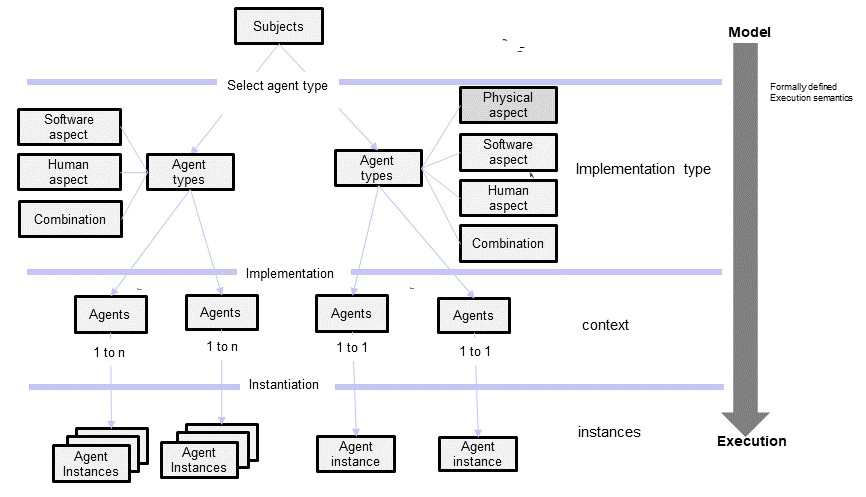
\includegraphics[width=0.9\linewidth]{Figures/Implementation/Implementation-steps.jpg}
	\caption[Implementation steps]{Implementation steps}
	\label{fig:Implementation-steps}
\end{figure}

In a system model, the actors, the actions, their sequences and the objects manipulated by the actions are described. Actions (activities) can be performed by humans, software systems, physical systems or a combination of these basic types of actors. We call them the task holders. For example, a software system can automatically perform the "tax rate calculation" action, while a person uses a software program to perform the "order entry" activity. The person enters the order data via a screen mask. The software checks the entered data for plausibility and saves it. However, activities can also be carried out purely manually, for example when a warehouse worker receives a picking order on paper, executes it, marks it as executed on the order form and returns it to the warehouse manager.\\
When creating a system model, it is often not yet known which types of actors execute which actions. Therefore, it can be useful to abstract from said CS: said?? the?  model when starting to describe processes by introducing abstract actors. A modeling language should allow the use of such abstractions. This means that when defining the process logic, no assertion should have to be made about what type of actor is realized. In S-BPM, the subjects represent abstract actors. \\
In the description of the control logic of a process, the individual activities are also described independently of their implementation. For example, for the action "create a picking order" it is not specified whether a human actor fills in a paper form or a screen mask, or whether a software system generates this form automatically. Thus, with activities the means by which something happens is not described, but rather only what happens.\\
The means are of course related to the implementation type of the actor. As soon as it has been defined which types of actors are assigned to the individual actions, the manner of realization of an activity has also been defined. In addition, the logical or physical object on which an action is executed also needs to be determined. Logical objects are data structures whose data is manipulated by activities. Paper forms represent a mixture between logical and physical objects, while a workpiece on which the "deburring" action takes place is a purely physical object. Therefore, there is a close relationship between the type of task holder, the actions and the associated objects actors manipulate or use when performing actions.\\
A system model can be used in different areas. The process logic is applied unchanged in the respective areas. However, it may be necessary to implement the individual actors and actions differently. Thus, in one environment certain actions could be performed by humans and in another the same actions could be performed by software systems. In the following, we refer to such different environments of use for a system model as context. Hence, for a process model, varying contexts can exist, in which there are different realization types for actors and actions.\\
In Subject Oriented Modeling, actors are not assigned to individual activities, but rather the actor type is assigned to an entire subject. This assignment is not part of the process logic, but in the most simple way it is done instead for each process in a separate two-column table. The left column contains the subject name and the right column the implementation type. If there are several contexts for a model, a separate assignment table is created for each of them.
The assignment of the implementation type forms the transition between the system logic and its implementation. Subsequently, it has to be defined which persons, software systems and physical systems represent the actors and how the individual actions are concretely realized. These aspects are described in detail in the following subsections.

\section{People and organizations}

This section describes how the organizational view of a company can be modeled formally and elements of it can be referenced with a modeling language.  Expressions of this language are stored in the subjects (the abstract actors) and resolved at runtime to a set of concrete actors. The actvities can then be assigned to them. 
The research presented here is able to represent any kind of resources of a company (people, software, machines etc.) and their arbitrary relationships amongst them. This way, the organizational structure of a company can be mapped very precisely.

The original idea of the approach goes back to Schaller's work  \cite{Schaller98}. Enhancements were made in the following articles \cite{Lawall2014, Lawall2014a, Lawall2014b, Lawall2014d, Lawall2014c, Lawall2013, Lawall2011}.

Let's start with the essential question whats makes up an organization. 


\subsection{What is an organization?}

\paragraph{Insights}
We are looking at a real world scenario in the context of an insurance company. 
A claims department usually has a manager, a number of clerks and a lawyer. Generally the lawyer is the deputy of the department head, cf. figure \ref{GeneralDep}.
	\begin{figure}[htb!]
	\centering
	\includegraphics[width=0.7\textwidth]{Figures/ExampleDepartmentGeneral.pdf}
	%\includegraphics[scale=0.65]{ExampleDepartmentGeneral.eps}
	\caption{Claims department in general}
	\label{GeneralDep}
	\end{figure}

We examined two concrete departments: one responsible for ``Car Damages'' the other responsible for ``House Damages''. Compared to the general structure and policies we observed some differences (cf. figure \ref{Example1}). At ``Car Damages'' there was an additional secretary position. In absence of the manager, organizational tasks were assigned to the secretary position. There was a change in the deputyship between the department head and the lawyer as well. Byron\footnote{We are using fantasy names.}, the lawyer, had been working in the department for only three weeks and therefore was not very experienced. The clerk Winter has been working in the department for over ten years. Based on that constellation the department head Smith decided that Winter should be his general deputy. Hinton was as well a deputy for Smith but only depending on some constraint information like the cash value of a claim for instance (constrained deputy relation in figure \ref{Example1}).

Looking at this two departments we also found an interesting mutual deputyship between the lawyers of the two departments (cf. figure \ref{Example1}). This observation gets important when thinking about dividing the organization system into types or classes on the one hand and instances on the other. Please note, that the relationships defined until now are specified on different levels of abstraction (positions and actors).
	\begin{figure}[htb!]
	\centering
	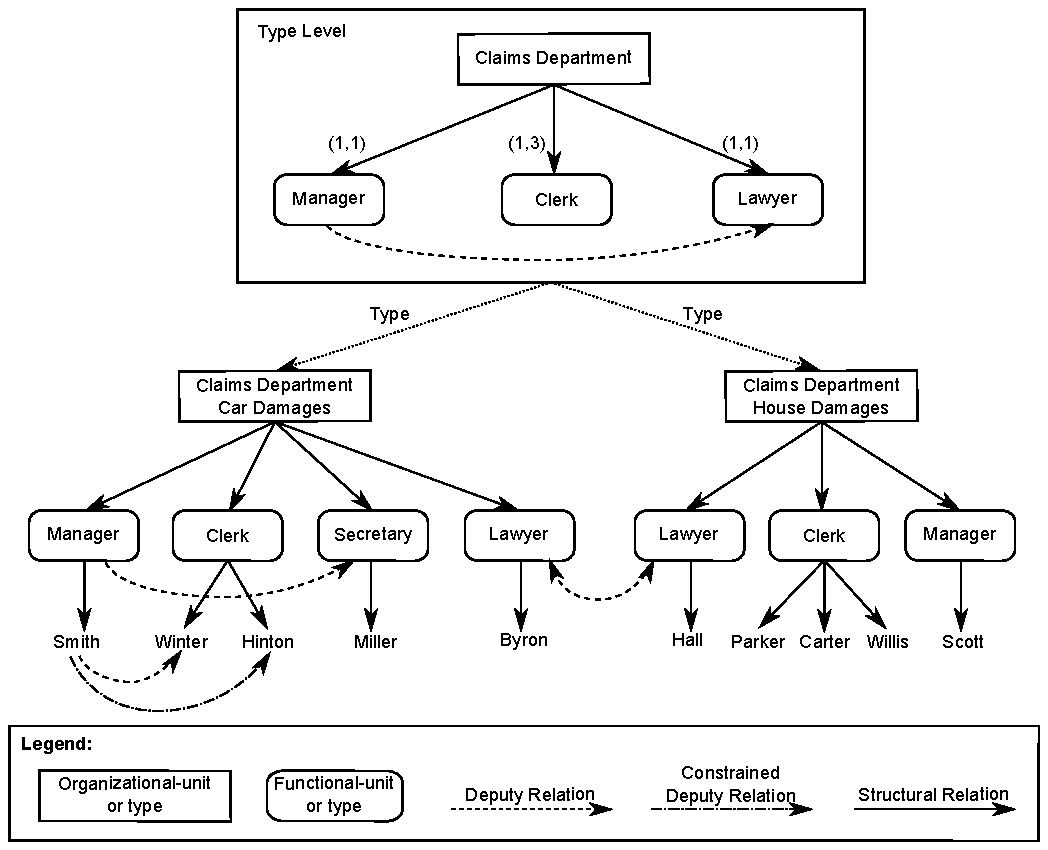
\includegraphics[width=\textwidth]{Figures/alles.pdf}
	\caption{Type and instance level of the example, adapted from \cite[fig. 3]{Lawall2013}}
	\label{Example1}
	\end{figure}

\subparagraph{Lessons Learned}

This section describes additional observations concerning real world organization policies\footnote{A complete overview can be found in \cite{Schaller98}.}.

\subparagraph{Knowledge Hierarchy}
As we have seen there are different levels of organizational knowledge. On the top level general structural assertions like ``a department consists of one to three clerks'' are dominant. We call this level the \emph{type} or \emph{template} level. Knowledge on this level is based on experience and is changed seldom as time goes by. Looking at real world departments -- we will call them \emph{instances} -- things become more concrete and specialized. There are concrete positions and the relationships between them. Finally, actors are assigned to the concrete positions. The organizational structures on this level are changing more frequently according to the demands of the daily business.

\subparagraph{Relationships}
An organization structure is formed by elements and relationships between them. It is important to realize the existence of several relationship types like ``is\_part\_of'', ``is\_deputy'', ``is\_supervisor'', ``reports\_to'' and so on.

Positions are abstractions of persons (actors) having a defined skill set fulfilling specific tasks. These abstractions help defining a more stable model of the organization that is independent from employee turnover. Relationships can be defined between abstract positions or on the concrete actor level.

Relationships are rarely of a general nature. As discussed in our example, relationships depend on specific constraint information like the cash value of a car claim. Even the ``is\_deputy''-relationship can depend on projects or products if you think in the terms of a matrix organization. They can also be only valid for a fixed time period.

\subparagraph{Multidimensional organizations}
Business organizations are multidimensional. Even in organizations that -- at first glance -- are structured hierarchically, there are structures belonging to the so called secondary (``shadow'') organization comprising committees, commissions, boards and so on. The positions and functions of the secondary organization are assigned to the employees. This leads to a multidimensional organization in every case. %We emphasize this point because there are some theories and approaches that are specific to hierarchical structures.

\subsection{Linking the process and the organizational model} \label{chapter_Linking}

Based on the organizational model, a server component is proposed that implements a special architecture and a unique algorithm for the resolution of expressions denoting abstract actors in the sense of subjects. This server is part of a greater system, the IT landscape of the company. ERP, process automation or database management systems can be other components of the landscape. Each of these systems uses mechanisms to map actors to tasks of processes or to permissions on data objects. Instead of maintaining such assignments for each system individually by total enumeration, we propose using an organizational server. This organizational server contains the organizational model. A formal language is used to formulate expressions that define the assignments. Clients send these expressions as requests to the organizational server and retrieve sets of real actors as reply (cf. figure \ref{architecture}). The server offers a versatile interface consisting of only one function \emph{dispatch} that returns a subset of the actors maintained within the organization model.

A major benefit of this approach is that the server forms the result set based on the current organizational model. This means that if actors change functions or relations, these changes have an immediate impact on the client systems. The language expressions remain unaltered. Before the organizational change, ``Manager(*)'' yields (according to fig. \ref{Example1}) the actors Smith and Scott. If Scott leaves the company and is replaced by Willis, the model is changed. Now, the same expression evaluates to Smith and the new manager Willis.

	\begin{figure}[htb!]
	\centering
	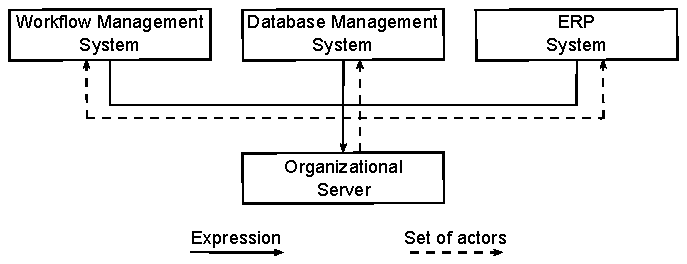
\includegraphics[scale=0.9]{Figures/architecture.pdf}
	\caption{Architecture}
	\label{architecture}
	\end{figure}

An informal overview on the functionality of the proposed server based on the introduced scenario could be assumed as the following. In a process management system a subject is defined by the expression  ``Manager(Claims Department Car Damages)''. At runtime the expression is passed to the organizational server. By traversing the organizational graph in figure \ref{Example1}, the algorithm moves to the department ``Claims Department Car Damages'' looking for a position ``Manager''. After that, the algorithm determines all the actors assigned to that position, finding manager Smith. If Smith is on the job, his identification is handed back to the workflow management system and the search ends. In case that Smith is not available (e.g. through vacation or sickness) the algorithm searches for  deputy relations between Smith and other actors. Obviously, there are two relations. If Winter \textbf{and} Hinton appear in the search result depends on the constraint on the relation to Hinton and whether they are on the job. In case of an empty set, the algorithm moves to the functional-unit manager looking 	for a deputy relation and finds the functional-unit secretary assigned to Miller. If Miller is on the job, her identification will be returned to the workflow management system. If not, the algorithm has the alternative of determining a valid deputy on the type level. Let us assume that the department is linked to the department type as depicted in figure \ref{Example1}. Within this type, the algorithm finds the lawyer as a deputy. It moves back to the instance ``Claims Department Car Damages'' and checks if there is a functional-unit with this name and an actor assigned to that functional-unit that is available. If Byron is on the job, his identification is returned. Otherwise, the lawyer of the ``Claims Department Car Damages'' has a two-way deputy relation with the lawyer of the ``Claims Department House Damages''. If this functional-unit has an actor assigned to itself and the actor is available, the algorithm will hand back his identification (here Hall, the lawyer of the ``Claims Department House Damages''). Otherwise the returned set is empty. In this case, the workflow management system has to postpone the execution of the task.


\section{Formal Specification}

The formalization of the organizational model is described using relations and integrity constraints. In the following we present a simplified model of Schaller's approach.

Within our meta-model an organization is a tuple O = ($name$, $\domaene$, $\OrgElementMenge$, $\relmenge$, $\relationen$) where $name$ denotes the modeled organization. The remaining symbols have the following semantics:

\subsection{Domains $\domaene$}
	$\domaene = \{ \Bezeichner, \zeit, \ID, \relname, \attribute, \WerteMenge, \praedikat \} $ is a set
	of domains consisting of the subsets:

	\begin{itemize}

	\item $\Bezeichner$ an organization specific set of terms describing the building blocks of the
	organization, like "`claims department"', department "`head"' and so on,

	\item $\zeit$ denotes a set of time values, like ``May 19th 2010 08:00:00''.

	\item $\ID$ a set of abstract identifiers.

	\item $\relname$ denotes a set of relationship names, "`deputy"' or "`reports\_to"' for instance.

	\item $\attribute$ a set of attributes used to detail the elements of our model. Attributes are mapped to model elements using the function  $val: \attribute \rightarrow \WerteMenge$ that assigns a value $w \in \WerteMenge$ to each
	$a \in \attribute$.

	\item	$\praedikat$ denotes a set of predicates like "`(ActualYear - HiringYear) $>$ 10"'.

	\end{itemize}

\subsection{Organization Elements $\OrgElementMenge$}
	The set $\OrgElementMenge = \oetyp \cup \ftyp \cup \oe \cup \f \cup \a $ comprises all the building blocks of an organization on the type as well as on the instance level. The elements of $\OrgElementMenge$ represent the nodes of the resulting organization graph.

	\begin{itemize}

	\item $\oetyp$ denotes the set of organizational-unit types, like departments or working groups.


	\item $\ftyp$ is the set of functional-unit types, like the ``manager'', ``lawyers''\ and so on.


	\item $\oe$ represents the set of organizational-units, like departments, committees, teams and so on. As already explained, organizational-units can have a relation to a type. The total function $type_{\oe}: \oe \rightarrow \oetyp \cup NULL$ returns the specific type for every organizational-unit.

	\item $\f$ is the set of functional-units, like positions or roles. There also exists a type function that is almost defined in the same manner as described above. The type of a functional-unit is returned by the function $type_F{\f}: \f \rightarrow \ftyp \cup NULL$.

	$\relstrukturOE_F \subset \oe \times (\oe \cup \f)$ denotes the is\_part\_of-relation between organizational- and functional-units.$\relstrukturOE_F$ on the one hand	describes the mapping of functional-units to organizational-units. On the	other hand the hierarchy between orga-nizational-units can be modeled. When focusing on the organizational-units the relation ${\relstrukturOE_F}^{'} = \relstrukturOE_F \rhd \oe$ has to be irreflexive and cycle-free. ${\relstrukturOE_F}^{''} = \relstrukturOE_F \rhd \f$ has to be surjective.

	\item  $R^{\f}$ denotes a set of user-defined relations. All members $r \in R^{\f}$ have the structure $r \subset (\f \times \f)$ and	are irreflexive.

	\item The set $\a$ denotes the actors: employees (users) and the computer systems. We explicitly model these computer systems because they can carry out tasks and therefore need permissions. $\relstrukturFA \subset \f \times \a$ is a relation and describes the assignments of employees to positions. As seen before, there is also a user-defined set of relationships $R^{\a}$. All relations $r \in R^{\a}$ have the structure $r \subset (\a \times (\a \cup \f))$. Further on, for all $r \in R^{\a}$ the condition $\forall r \in R^{\a}: \left[(x,y) \in r \rightarrow x \neq y \right]$ holds, meaning that every relation	$r \in R^{\a}$ is cycle-free.

	\item Additionally every element of $\OrgElementMenge$ is described as tuple $(id, name)$, with $id \in \ID$ and $name \in \Bezeichner$.

	\end{itemize}

\subsection{Set of Relations $\relmenge$}
	$\relmenge$ denotes a set of relation sets and is defined as
	$\relmenge = \relmengetyp \cup \relmengeinst$, with:

	\begin{itemize}

	\item $\relmengetyp$ denotes the set of relations defined between the types of organizational- and functional-units.
	$\relmengetyp$ is defined as $\relmengetyp = \typstrukturrelation \cup \typbenutzerrelationenmenge$, with:
	\begin{itemize}

		\item $\typstrukturrelation \subset \oetyp \times (\oetyp \cup \ftyp)$ is the ``is\_part\_of''-relation on the type level. Concerning the structure between the elements of $\oetyp$, there are some restrictions. Let's say ${\typstrukturrelation}^{'} = \typstrukturrelation \rhd \oetyp$\footnote{The operator $\rhd$ is defined as $((\rel \subset A \times B) \rhd (C \subset B)) := \{(x,y) \in \rel \, \vert \, y \in C \}$.}.
		An organizational-unit type can not be his own successor. ${\typstrukturrelation}^{'}$ therefore has to be irreflexive and cycle-free.
		Let's have a look at the functional-unit types. Obviously the relationship between $\oetyp$ and $\ftyp$ can be described as ${\typstrukturrelation}^{''} = \typstrukturrelation \rhd \ftyp$. Since organizational-unit types combine functional-unit types, ${\typstrukturrelation}^{''}$ has to be total. On the other side, every $f \in \ftyp$ has to be linked to an organizational-unit type $o \in \oetyp$. ${\typstrukturrelation}^{''}$ therefore has to be surjective.

		\item As explained above, there is the need for a flexible integration of new relation-types into the model. Therefore we define a set of relation-types $\typbenutzerrelationenmenge$. Every relationship $\typbenutzerrelation \in R^{\typsymbol}$ has the structure $\typbenutzerrelation \subset (\ftyp \times \ftyp) \times \praedikat$ and can further be constraint using predicates to restrict the set of valid functional-unit types and therefore the set of valid users\footnote{Please take a look at the relation $\relstrukturFA$ and its according constraints}. Please note that $\typbenutzerrelation$ is used as variable. The relations between the functional-unit types, that can expressed using the term $dom(\typbenutzerrelation)$, are irreflexive. Defining a deputyship between one node and itself is not very meaningful for instance. Concerning the predicates we additionally postulate that each $\typbenutzerrelation \in \typbenutzerrelationenmenge$ has to be a function, assigning each ordered pair $(f,f) \in \ftyp \times \ftyp$ a unique predicate $p \in \praedikat$.

	\end{itemize}
	\item $\relmengeinst$ defines several relations between organizational- and functional-unit types as well as actors. We declare $\relmengeinst$ as 		$\relmengeinst = \relmengeinstOE_F \cup \relmengeinstFA$, with:

		\begin{itemize}

		\item $\relmengeinstOE_F = \relstrukturOE_F \cup \relmengebenutzerinstOE_F$ the set of relations between organizational- and functional-units, with:
			\begin{itemize}
			\item $\relstrukturOE_F \subset \oe \times (\oe \cup \f)$ denotes the ``is\_part\_of''-relation between organiza-tional- and functional-units. On the one hand the relation describes the functional-units belonging to an organizational-unit, on the other hand the organization structure between the units themselves. Let ${\relstrukturOE_F}^{'} = \relstrukturOE_F \rhd \oe$ denote the structure between the organizational-units. According to our description ${\relstrukturOE_F}^{'}$ has to be irreflexive and cycle-free. In the same manner and similar to our definition of ${\typstrukturrelation}^{''}$,${\relstrukturOE_F}^{''} = \relstrukturOE_F \rhd \f$ has to be total and surjective.

			\item $\relmengebenutzerinstOE_F$ is a set of user-defined relations. Every single relation ${\relbenutzerinstOE_F}$ within $\relmengebenutzerinstOE_F$ has the structure ${\relbenutzerinstOE_F} \subset \f \times \f$ and is irreflexive.
			\end{itemize}

		\item $\relmengeinstFA$ denotes a set of relations between functional-units and actors. $\relmengeinstFA$ is defined as $\relmengeinstFA = \relstrukturFA \cup \relmengebenutzerFA$, with:

			\begin{itemize}

			\item $\relstrukturFA \subset \f \times \a$ describes the function assignments of the actors. We demand that every actor is named to at least one function.

			\item $\relmengebenutzerFA$ a set of user-defined, irreflexive relations 	${\relbenutzerFA}$ having the structure $\forall {\relbenutzerFA} \in \relmengebenutzerFA: {\relbenutzerFA} \subset \a \times (\a \cup \f)$. For every $\relbenutzerFA \in \relmengebenutzerFA$ the condition		$\left[(x,y) \in \relbenutzerFA \rightarrow x \neq y \right]$ holds.
			\end{itemize}

		\end{itemize}

	\end{itemize}

	All elements of our model can be detailed using time constraints and attributes.

\subsection{Additional relations $\relationen$}

	$\relationen$ consists of several relations and is defined as $\relationen =\{ \rel_{Time}, \rel_{\attribute},$ $\rel_{Card}, \rel_{val}, \rel_{Name}\}$, with:

	\begin{itemize}
	\item $\rel_{Time} \subset \bigl( \OrgElementMenge \cup \relmenge \bigr)\times \bigl( \zeit \times \zeit \bigr)$ describes the duration of validity of every single organizational element in our model. $\rel_{Time}$ therefore has to be a total relation.

The two functions $start$ and $stop$ denote the birth and death of an organizational element. We define these functions as:
			$$
			\begin{array}{cll}
			start: \bigl( \OrgElementMenge \cup \relmenge \bigr) \rightarrow \zeit, &
				\mbox{with the semantic} & \\
				& start(x \in ( \OrgElementMenge \cup \relmenge ) ) =
				dom( ran ( x \lhd \rel_{Time})) & \\
			stop: \bigl( \OrgElementMenge \cup \relmenge \bigr) \rightarrow \zeit, &
				\mbox{with the semantic} & \\
				& stop(x \in ( \OrgElementMenge \cup \relmenge ) ) =
				ran( ran ( x \lhd \rel_{Time})) & \\
			\end{array}
			$$
It is obvious that the following constraint should hold: $\forall x \in \bigl( \OrgElementMenge \cup \relmenge \bigr): start(x) \leq stop(x)$.  In order to define an existence ad infinitum we introduce the symbol ``$*$''\ concerning the value of the $stop$ function.

	\item $\rel_{\attribute} \subset \bigl( \OrgElementMenge \cup \relmenge \bigr) \times \attribute$ assigns attributes to our organizational elements.
		$\rel_{\attribute}$ is a surjective relation. Thus every attribute can only be assigned to one organizational element.

	\item $\rel_{Card} \subset \typstrukturrelation \times (\natnull \times \natnull)$ assigns cardinalities to our ``is\_part\_of''-relation between organizational- and functional-unit types. $\rel_{Card}$ is a total and unique relation.

		As abbreviations we define the functions $min$ and $max$, with
		$$
		\begin{array}{cl}
		min: \typstrukturrelation \rightarrow \natnull, & \mbox{with the semantic} \\
		& min(r \in \typstrukturrelation) = dom( ran( r \lhd \rel_{Card})) \\
		max: \typstrukturrelation \rightarrow \natnull, & \mbox{with the semantic} \\
		& max(r \in \typstrukturrelation) = ran( ran ( r \lhd \rel_{Card}))
		\end{array}
		$$
		Additionally we demand $\forall r \in \typstrukturrelation: min(r) \leq max(r)$.

	\item Via $\rel_{val} \subset \praedikat \times (\f^{\typsymbol} \cup A)$ each predicate, its typed functional-unit and actors is assigned. The predicate {\em true} holds for all typed functions and actors and we define $\forall x \in \f^{\typsymbol} \cup A: \quad (true, x) \in \rel_{val}$.

	\item $\rel_{Name} \subset \bigl( \typbenutzerrelationenmenge \cup \relmengebenutzerinstOE_F \cup \relmengebenutzerFA \bigr) \times \relname$
		assigns names to our user-defined relations. None of these relations should be nameless. $\rel_{Name}$ therefore has to be total and unique.
		As already mentioned, $\typstrukturrelation, \relstrukturOE_F$ and	$\relstrukturFA$ denote ``is\_part\_of''-relations. A specific naming of these 		relations is therefore unnecessary.
\end{itemize}

\subsection{Policy Resolution}\label{PolicyResolutionFormal}

As discussed in section \ref{chapter_Linking} our organizational server offers an interface with a very small footprint, consisting only of the function "`dispatch"'. The function returns a subset of the actors fulfilling the language expression in conjunction with conditions. These conditions are formulated via the following parameters expected by the function.
\begin{itemize}
	\item a set of organizational-unit names $oe_{bez} \in \Bezeichner$,
	\item a set of tuples consisting of attributes and corresponding values $attr_{oe} \subset (\Bezeichner \times \WerteMenge)$ belonging to defined organizational-units,
	\item a set of functional-unit names $f_{bez} \in \Bezeichner$,
	\item a set of tuples consisting of attributes and corresponding values $attr_{f} \subset (\Bezeichner \times \WerteMenge)$ belonging to functional-units,
	\item a set of actor names $a_{bez} \in \Bezeichner$,
	\item a set of tuples consisting of attributes and related values $attr_{a} \subset (\Bezeichner \times \WerteMenge)$, belonging to actors,
	\item the name of a relation $rel \in \relname$ and
	\item a set of tuples consisting of attributes and corresponding values $attr_{rel} \subset (\Bezeichner \times \WerteMenge)$, belonging to that relation.
\end{itemize}

%The {\tt dispatch}-algorithm works as follows:

	\begin{samepage}
	{\small
	\NumberProgramstrue
	\begin{algorithm}[dispatch]\label{alg:GetIt}
	\begin{program}
	\FUNCT |dispatch|(oe_{bez} \subset \Bezeichner, attr_{oe} \subset (\Bezeichner \times \WerteMenge),
	f_{bez} \subset \Bezeichner, attr_f \subset (\Bezeichner \times \WerteMenge),
	a_{bez} \subset \Bezeichner, attr_a \subset (\Bezeichner \times \WerteMenge),
	rel \in \relname, attr_{rel} \subset (\Bezeichner \times \WerteMenge)) \subset \a
	\BEGIN
	\var \seq{oe \subset \oe; f \subset \f; a \subset A};
	/*|First we have to determine the existing organizational elements|*/
	oe := (\oe \rhd oe_{bez});
	f := (\f \rhd f_{bez});
	a := (A \rhd a_{bez});
	\IF (oe \neq \{\} \vee attr_{oe} \neq \{\}) \label{alg:GetIt:CallGetATbyOE}
	\THEN \RETURN \quad GetATbyOE(oe, attr_{oe}, f, attr_f, rel, attr_{rel})
	\FI
	\IF (f \neq \{\} \vee attr_f \neq \{\})
	\THEN \RETURN \quad GetATbyF(f, attr_f, attr_a, rel, attr_{rel})
	\FI
	\IF (a \neq \{\} \vee attr_a \neq \{\})
	\THEN \RETURN \quad GetAT(a, attr_a, rel, attr_{rel})
	\FI
	\RETURN \{\};
	\END
	\end{program}
	\end{algorithm}
	\NumberProgramsfalse
	}
	\end{samepage}

\noindent The execution of {\tt dispatch(\{Claims Department Car Damages\},\{\},\{Clerk\},\\ \{\},\{\},\{damage sum $<$ \$100\},\{\},\{\})} is equivalent to search all clerks in the organizational-unit {\it car damages} that are authorized to sign claims with a damage sum lower than 100 dollars. The execution will lead to a call of the {\tt GetATbyOE}-function. Based on the values of $oe$, $f$ and $a$ {\tt GetATbyOE} determines the organization elements fulfilling the remaining conditions specified in $attr_{oe}$, $attr_{f}$ and so on.

	%\longpage
	\begin{samepage}
	{\small
	\NumberProgramstrue
	\begin{algorithm}[GetATbyOE]\label{alg:GetATbyOE}
	\begin{program}
	\FUNCT |GetATbyOE|(oe \subset \oe, attr_{oe} \subset (\Bezeichner \times \WerteMenge), f \subset \f,
	attr_{f} \subset (\Bezeichner \times \WerteMenge), rel \in \relname, attr_{rel} \subset (\Bezeichner \times \WerteMenge),
	attr_a \subset (\Bezeichner \times \WerteMenge)) \subset \a
	\BEGIN
	\var \seq{f^{'} \subset \f; oe_{successor},oe_{successor}^{'} \subset \oe;
		o_{p} \subset \oe \times \oe};
	%=====================================================================================
	%\IF attr_{oe} = \{\} \THEN attr_{oe} = \attribute \FI \label{alg:GetATbyOE:kritisch1}
	%=====================================================================================
	/* o_{p}| denotes the vector corresponding to oe|*/;
	o_{p} := \{(x,y) \vert x \in oe \wedge y \in \oe \};\label{alg:GetATbyOE:Vektor}
	oe_{successor} := dom \left( \left({\left({\left({\relstrukturOE_F}^{'}\right)}^{*}\right)}^{T}\right) \circ o_{p} \right);\label{alg:GetATbyOE:Nachfolger}
	\IF (oe_{successor} = \{\})
	\THEN oe_{successor} := \oe; \label{alg:GetATbyOE:kritisch2}
	\FI
	%=======================================================================================
	%oe_{Nachfolger}^{'} := dom( \{ oe_{Nachfolger} \} \lhd \rel_{\attribute} \rhd attr_{oe} )
	%=======================================================================================
	oe_{successor}^{'} := GetOrgElements( oe_{successor}, attr_{oe});
	\IF (f = \{\})\label{alg:GetATbyOE:fIstNull}
	\THEN
		/*|determine all functional-units of the organizational-units|*/
		f^{'} := ran ( \{oe_{successor}^{'}\} \lhd \relstrukturOE_F ) \cap F;
		\RETURN \quad |GetATbyF|(f^{'}, attr_{f}, attr_a, rel, attr_{rel});
	\ELSE \label{alg:GetATbyOE:fIstNichtNull}
		/*|which of the preselected functional-units belong to|*/
		/*|the organizational-units determined in |oe_{successor}^{'}?*/
		f^{'} := ran ( \{oe_{successor}^{'}\} \lhd \relstrukturOE_F \rhd \{f\}) \cap F;
		\RETURN \quad |GetATbyF|(f^{'}, attr_{f}, attr_a, rel, attr_{rel});
	\FI
	\RETURN \quad \{\};
	\END
	\end{program}
	\end{algorithm}
	\NumberProgramsfalse
	}
	\end{samepage}

\noindent Line \ref{alg:GetATbyOE:Vektor} describes the declaration of a relational vector. The calculation of all successors in line \ref{alg:GetATbyOE:Nachfolger} is obtained by multiplying the transpose of the irreflexive closure of ${\relstrukturOE_F}^{'}$ with our vector $o_{p}$. After that we select the appropriate organizational-units.\\

In the case of the functional-unit set $f$ passed to our function is empty, the algorithm selects all functional-units of the calculated transitive-reflexive closure and calls the function {\tt GetATbyF} (line \ref{alg:GetATbyOE:fIstNull}). If $f$ != $\{\}$ the relevant functional-units are selected in dependency on the specified organizational-units. After that the function {\tt GetATbyF} is called	(line \ref{alg:GetATbyOE:fIstNichtNull}).

	%\longpage
	\begin{samepage}
	{\small
	\NumberProgramstrue
	\begin{algorithm}[GetATbyF]\label{alg:GetATbyF}
	\begin{program}
	\FUNCT |GetATbyF|(f \subset \f, attr_f \subset (\Bezeichner \times \WerteMenge), attr_a \subset (\Bezeichner \times \WerteMenge),
	rel \in \relname, attr_{rel} \subset (\Bezeichner \times \WerteMenge)) \subset \a
	\BEGIN
	\var \seq{f^{'},f^{''} \subset \f; a \subset A};
	\IF (attr_f = \{\})
	\THEN attr_f := \attribute;
	\FI
	f^{'} := f;
	\IF (f^{'} = \{\})
	\THEN f^{'} := \f;
	\FI
	%==========================================================
	%f^{'} := dom ( \{f\} \lhd \rel_{\attribute} \rhd attr_f );
	%==========================================================
	f^{''} := GetOrgElements( f^{'}, attr_f );
	a := ran( f^{''} \lhd \relstrukturFA );
	\RETURN \quad |GetAT|(a, attr_a, rel, attr_{rel});
	\END
	\end{program}
	\end{algorithm}
	\NumberProgramsfalse
	}
	\end{samepage}

\noindent Function {\tt GetATbyF} determines the set of functional-units fulfilling the attributes passed over as parameters first. After that corresponding actors are selected and handed over to {\tt GetAT}.\\

Algorithm \ref{alg:GetAT} describes the core idea of our system. The passed parameters are being processed from the actor level up to level of organizational- and functional-unit types. Individual rules therefore have a higher priority than policies specified on the more abstract type level.

	{\small
	\NumberProgramstrue
	\begin{algorithm}[GetAT]\label{alg:GetAT}
	\begin{program}
	\FUNCT |GetAT|(a \subset \a, attr_a \subset (\Bezeichner \times \WerteMenge), rel \in \relname, attr_{rel} \subset (\Bezeichner \times \WerteMenge)) \subset \a
	\BEGIN
	\IF (attr_a = rel = attr_{rel} = \{\})\label{alg:GetAT:trivial}
	\THEN \RETURN \quad a;
	\FI
	/* |exit for recursions| */
	\IF (attr_a \neq \{\} \wedge (rel = attr_{rel} = \{\})) \label{alg:GetAT:Aussprung}
	\THEN
		\IF a = \{\} \THEN a := \a \FI \label{alg:GetAT:A-Erweiterung}
		%=======================================================================================
		%a := dom \bigl( \{a\} \lhd \rel_{\attribute} \rhd \{attr_a\} \bigr); \label{alg:GetAT:1}
		%=======================================================================================
		\RETURN \quad  GetOrgElements( a, attr_a ); \label{alg:GetAT:1}
	\FI
	\IF rel \neq \{\} \label{alg:GetAT:komplex}
	\THEN
		\IF a = \{\} \THEN a := \a \FI
		%=======================================================================================
		%\IF attr_{rel} = \{\} \THEN attr_{rel} := \attribute \FI
		%=======================================================================================
		\var \seq{\rel_x, \rel_x^{'} \in \relmengebenutzerFA; y \subset (\f \cup \a)};
		/* | is there a user-defined relation fulfilling the attributes?|*/
		%\rel_x^{'} := name^{-1}(rel) \cap \relmengebenutzerFA; \label{alg:GetAT:FA}
		\rel_x^{'} := dom(\rel_{Name} \rhd rel) \cap \relmengebenutzerFA; \label{alg:GetAT:FA}
		%=======================================================================================
		%\rel_x := dom(\{\rel_x^{'}\} \lhd \rel_{\attribute} \rhd attr_{rel});
		%=======================================================================================
		\rel_x := GetOrgElements( \rel_x^{'}, attr_{rel});
		\IF \rel_x \neq \{\}
		\THEN
		%=======================================================================================
		%	z := ran ( dom ( (\{a\} \lhd \rel_x) \lhd \rel_{\attribute} \rhd \{attr_{rel}\} ) );
		%=======================================================================================
			\var \seq{z \subset A \cup \f; w,y \subset A};
			z := ran( GetOrgElements(\{a\} \lhd \rel_x, attr_{rel}) );
			/*| select the actors according to |$z$
			w := z \cap \a;
			/*| select the actors according to | \relstrukturFA */
			y := ran (\{ \{z\} \cap \f\} \lhd \relstrukturFA);
			\RETURN \quad w \cup y;
		\ELSE
			\var \seq{\rel_x^\f, {\rel_x^\f}^{'} \subset \relmengebenutzerinstOE_F};
			%{\rel_x^\f}^{'} := name^{-1}(rel) \cap \relmengebenutzerinstOE_F; \label{alg:GetAT:FF}
			{\rel_x^\f}^{'} := dom(\rel_{Name} \rhd rel) \cap \relmengebenutzerinstOE_F; \label{alg:GetAT:FF}
			%===================================================================================
			%\rel_x^\f := dom(\{{\rel_x^\f}^{'}\} \lhd \rel_{\attribute} \rhd attr_{rel});
			%===================================================================================
			\rel_x^\f := GetOrgElements({\rel_x^\f}^{'}, attr_{rel});
			\IF \rel_x^\f \neq \{\}
			\THEN
				\var \seq{a^{'} \subset A};
				/*|select all actors connected to the functional-unit |*/
				a^{'} := ran \left( \{ ran \left( \rel_x^\f \right) \} \lhd \relstrukturFA \right);
				\RETURN \quad |GetAT|(a^{'}, attr_a, \{\},\{\});
			\ELSE /*|lookup in the  type level|*/
			\var \seq{\rel_x^\ftyp,{\rel_x^\ftyp}^{'} \subset \typbenutzerrelationenmenge};
			%{\rel_x^\ftyp}^{'} := name^{-1}(rel) \cap \typbenutzerrelationenmenge; \label{alg:GetAT:FtFt}
			{\rel_x^\ftyp}^{'} := dom(\rel_{Name} \rhd rel) \cap \typbenutzerrelationenmenge; \label{alg:GetAT:FtFt}
			%===================================================================================
			%\rel_x^\ftyp := dom(\{{\rel_x^\ftyp}^{'}\} \lhd \rel_{\attribute} \rhd attr_{rel});
			%===================================================================================
			\rel_x^\ftyp := GetOrgElements({\rel_x^\ftyp}^{'}, attr_{rel});
			\IF \rel_x^\ftyp \neq \{\}
			\THEN
				\var \seq{f^{'},f^{''} \subset \f; a^{'},a^{''},a^{'''} \subset A};
				/*|1. address all true relationships |*/ \label{alg:GetAT:PraedikateStart} \label{alg:GetAT:WahrePraedikate}
				%/*|mit dem Pr"adikat "`wahr"'|*/
				f^{'} := dom \bigl( type_F^{\typsymbol} \rhd ran( dom (\rel_x^\ftyp \rhd \{wahr\}))\bigr);
				a^{'} := ran \bigl( f^{'} \lhd \relstrukturFA \bigr);
				/*|2. address false relationships |*/\label{alg:GetAT:NichtWahrePraedikate}
				%/*|Pr"adikaten ungleich "`wahr"'|*/
%				/* */
				/*|2.1 address typed functional-units |*/
				f^{''} := dom \bigl( \bigl( type_F^{\typsymbol} \rhd ran( dom (\rel_x^\ftyp \rrhd wahr\})) \bigr)
				\cap
				ran \bigl( ran(\rel_x^\ftyp \rrhd \{wahr\}) \lhd \rel_{val} \bigr) \bigr);
				a^{''} := f^{''} \lhd \relstrukturFA;
				/*|2.2 address direct relationships|*/
			a^{'''} :=
				\bigl( dom \bigl( type_F^{\typsymbol} \rhd ran( dom (\rel_x^\ftyp \rrhd \{wahr\})) \lhd \relstrukturFA \bigr)
				  \cap ran \bigl(  ran(\rel_x^\ftyp \rrhd \{wahr\}) \lhd \rel_{val} \bigr) \bigr);
				\RETURN \quad |GetAT|(a^{'} \cup a^{''} \cup a^{'''}, attr_a, \{\},\{\}); \label{alg:GetAT:PraedikateStop}
			\ELSE
				/*| no corresponding relationship found |*/

				\RETURN \quad \{\};
			\FI
		\FI
	\FI
	\FI
	\END
	\end{program}
	\end{algorithm}
	\NumberProgramsfalse
	}

\noindent Line \ref{alg:GetAT:trivial} describes the trivial case. If the only parameter is a set of actors the return value will be the same set.\\

In case that attributes are handed over (that have to be fulfilled by the respective actors) and no user-defined relation was defined (line~\ref{alg:GetAT:Aussprung}), the algorithm determines all actors with a fulfilling attribute set. If $a$ is empty, all actors (line \ref{alg:GetAT:A-Erweiterung}) are used within the search (line \ref{alg:GetAT:1}). \\

The core concept of the algorithm starts with line \ref{alg:GetAT:komplex}. The following user-defined relations have to be resolved:
\begin{itemize}
	\item The relation between actors and functional-units ($\relmengebenutzerFA$),
	\item The relation between functional-units ($\relmengebenutzerinstOE_F$) and
	\item The relation between functional-unit types ($\typbenutzerrelationenmenge$)
\end{itemize}

If no corresponding relation on the actor level can be found (line \ref{alg:GetAT:komplex}), the algorithm checks for a connection between two functional-units ($\relmengebenutzerinstOE_F$) in order to retrieve the attached actors. If no match is possible, the algorithm searches for a relation on the more abstract type level (line \ref{alg:GetAT:FtFt}). If a relation can be found these policies are used for retrieving matching actors on the instance level. Lines \ref{alg:GetAT:PraedikateStart} to \ref{alg:GetAT:PraedikateStop} show the semantics of the predicates $p \in \praedikat$ of the relation $\typbenutzerrelation \in \typbenutzerrelationenmenge$. All not predicate constrained relations are evaluated (line \ref{alg:GetAT:WahrePraedikate}), first. After that the algorithm examines the constrained relations (line \ref{alg:GetAT:NichtWahrePraedikate}).  The resulting actor set is used for a recursive call of algorithm \ref{alg:GetAT}.\\

\noindent Algorithm {\tt GetOrgElements} selects those elements fulfilling a defined attribute set $attr$ from the set of organizational-units and relations.

	%\longpage
	\begin{samepage}
	{\small
	\NumberProgramstrue
	\begin{algorithm}[GetOrgElements]\label{alg:GetOrgElements}
	\begin{program}
	\FUNCT |GetOrgElements|(k \subset \OrgElementMenge \cup \relationen, attr \subset (\Bezeichner \times \WerteMenge)) \subset \OrgElementMenge \cup \relationen
	\BEGIN
	\var \seq{ x \subset \OrgElementMenge \cup \relationen};
	x := \{\};
	\FOREACH y \in k~\DO
		\IF CheckAttributes(y, attr)
		\THEN
			x := x \cup y;
		\FI
	\OD
	\RETURN \quad x;
	\END
	\end{program}
	\end{algorithm}
	\NumberProgramsfalse
	}
	\end{samepage}

\noindent The following algorithm checks if an attribute of set $attr$ is mapped to an organizational element or relation $k \in \OrgElementMenge \cup \relationen$.

	\begin{samepage}
	{\small
	\NumberProgramstrue
	\begin{algorithm}[CheckAttributes]\label{alg:CheckAttributes}
	\begin{program}
	\FUNCT |CheckAttributes|(k \in \OrgElementMenge \cup \relationen, attr \subset (\Bezeichner \times \WerteMenge)) \subset \boole
	\BEGIN
	\var \seq{attr_k \subset \attribute};
	\IF (attr = \{ \})
		\THEN \RETURN \quad \true;
	\ELSE
		attr_k := ran( k \lhd \rel_{\attribute});
		\IF ( dom(attr) \subset ran( attr_k ))
		\THEN
			\FOREACH y \in attr~\DO
				\IF (ran(y) \neq val(attr_k \rhd dom(y)))
				\THEN \RETURN \quad \false;
				\FI
			\OD
			\RETURN \quad \true;
		\ELSE \RETURN \quad \false;
		\FI
	\FI
	\END
	\end{program}
	\end{algorithm}
	\NumberProgramsfalse
	}
	\end{samepage}

\noindent If the required attributes and attribute values are mapped to an organizational element or relation, function {\tt CheckAttributes} returns $true \in \boole$, or otherwise $false \in \boole$. $\boole = \{ true, false \}$ denotes the set of boolean values.

\section{Implementation}
The formalism discussed in this contribution is implemented in a prototype. Figure \ref{proto-gui} depicts part of this implementation -- the graphical user interface (GUI). It contains a \emph{model} editor, a \emph{search} area, a \emph{tree-navigation} as well as an \emph{attribute pane} and a \emph{relation list} for a selected organizational element.

\begin{figure}
\centering
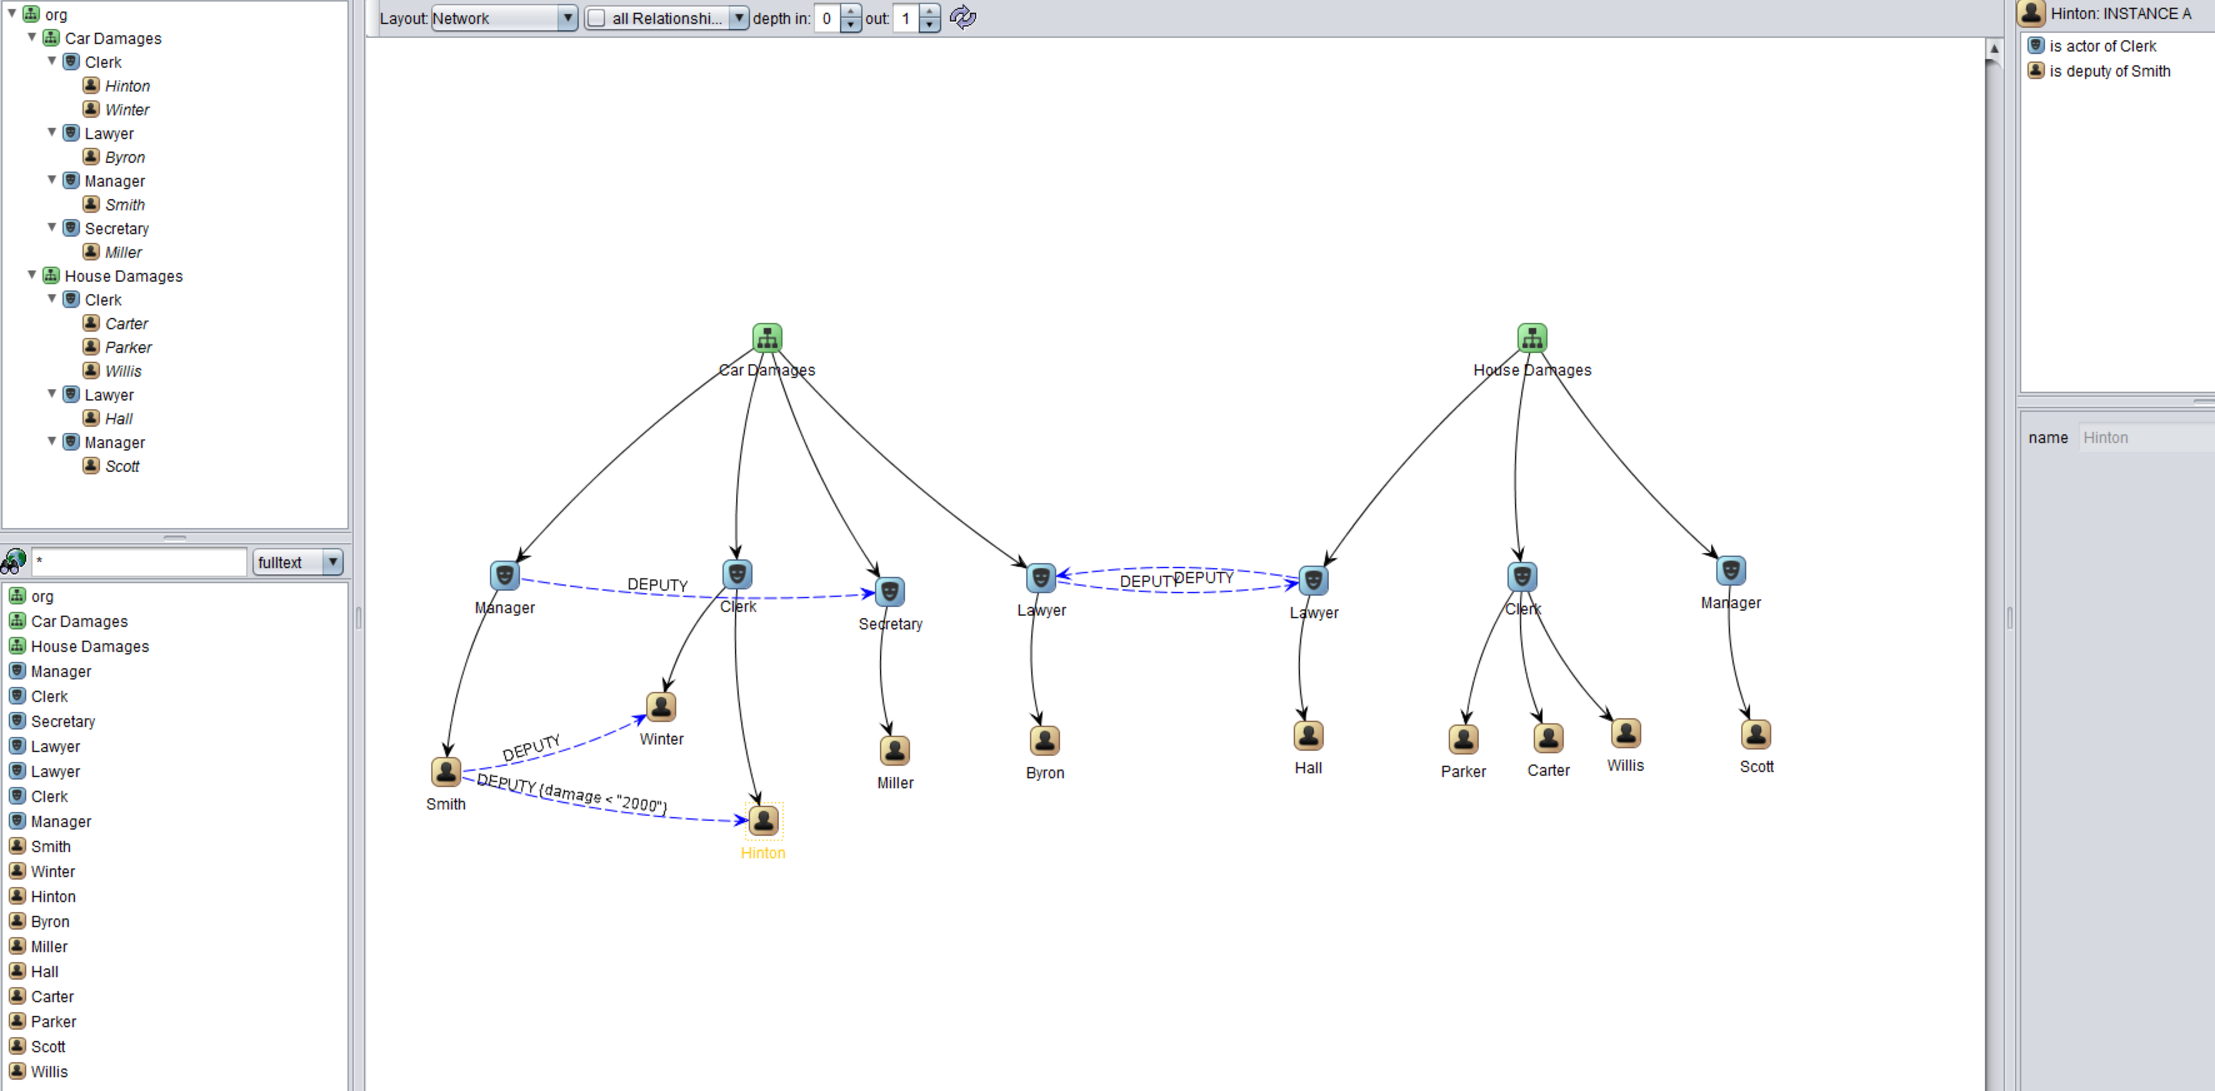
\includegraphics[width=\textwidth]{Figures/corg}
\caption{Screenshot: Implementation of the $\mathcal{C-ORG}$} GUI
\label{proto-gui}
\end{figure}

\begin{description}
  \item[The \emph{model editor}] provides a graph-based view on the organizational structure. Organizational elements are represented as nodes and their relations as edges. It provides means to navigate the model by centering on selected nodes. As the central component of the user interface, it is discussed below in more detail.
	\item[The \emph{search area}] can be used to retrieve a list of organizational elements. It has two modes of operation:
	  \begin{enumerate}
		  \item It provides a simple text index search for attribute values, e.g. entering ``Wi*'' will yield Winter and Willis.
			\item It can also be used to evaluate language expressions based on the approach described in section  and \ref{PolicyResolutionFormal}. An expression is entered and the result set for the current state of the organizational model is shown.
		\end{enumerate}
	\item[The \emph{tree-navigation}] projects the concrete organizational structure on a tree. Consequently, entities are duplicated in the projection if they can be reached on different paths.
	\item[The \emph{attribute pane}] in the bottom right section shows the attributes of the currently selected node or relation. It allows a quick modification, e.g. the assignment of a predicate to a relation.
	\item[The \emph{relation list}] lists all relations of the currently selected node, independent from the relation-types hidden in the model editor. This allows access to connected nodes and significantly reduces the time required to alter existing relations.
\end{description}

For quick access, elements can be dragged from any of the outer GUI sections and dropped into the model editor. If the elements have existing relations to the nodes already shown in the model editor, these relations will be shown as well. Otherwise, the elements are represented as unconnected nodes.

\begin{figure}
\centering
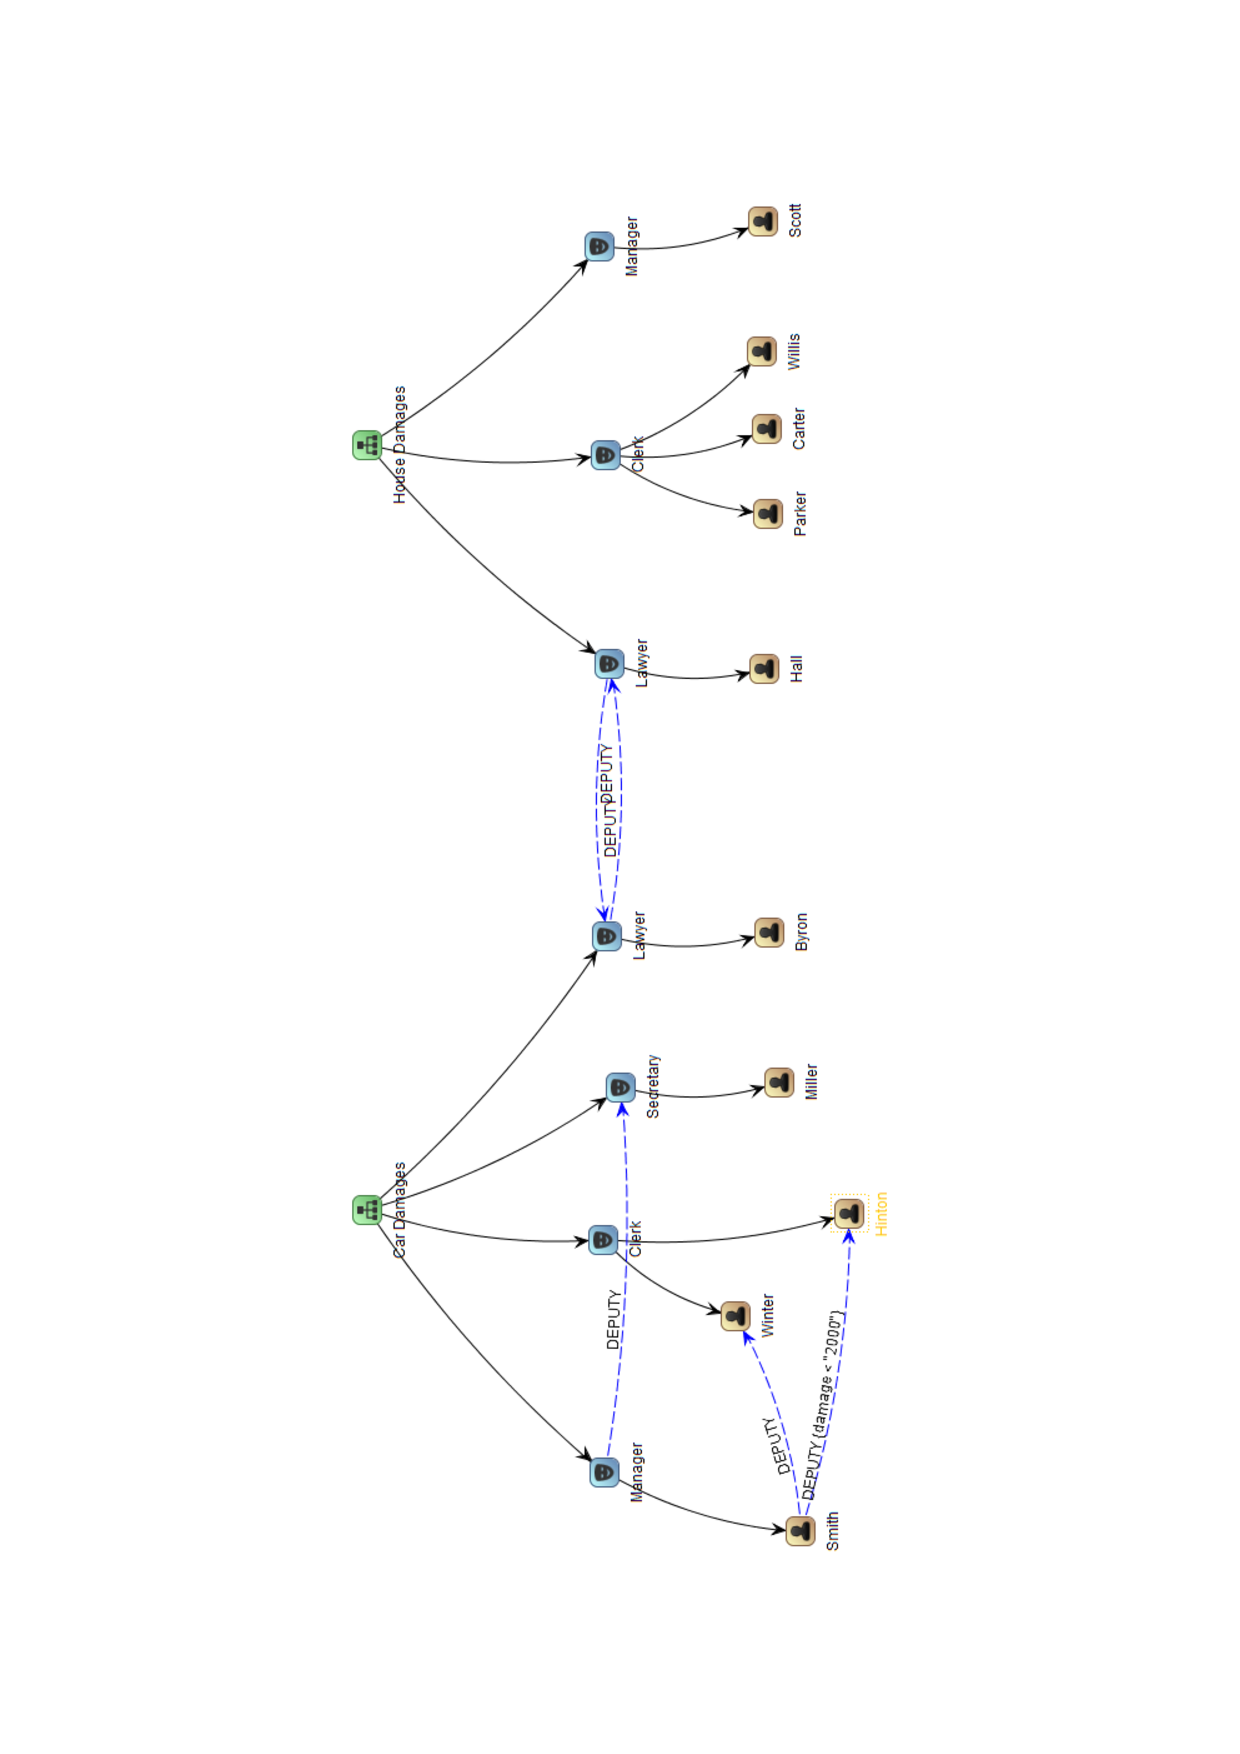
\includegraphics[width=\textwidth]{Figures/corg-graph.pdf}
\caption{Model Region of the Implementation}
\label{proto-model}
\end{figure}

Figure \ref{proto-model} provides an enlarged view of the model editor\footnote{It shows the example model (cf. fig. \ref{Example1}). The type level is hidden.}.
Users perform most modifications of the organizational model via this component.
In addition to navigating the model, they can create, modify and delete organizational elements and their interconnections.

It contains the model with the desired\footnote{The relation-types to be shown can be selected.} relations. The editor also shows concrete constraints (predicates) on relations, e.g. the deputy relation with \emph{damage $<$ ``2000''} between \emph{Smith} and \emph{Hinton}.


In addition to the user interface, the implementation provides a service that can accept language expressions from client systems. This interface is based on the Representational State Transfer (REST) paradigm.



\section{Physical infrastructure}

\todo{Bibtex-File muss noch angepasst werden.}

The previous remarks always referred to human actors. But executors in a business process can also be machines or software components. We will therefore look at how the concept presented in the previous chapters can be extended to the area of non-human actors. Here, the already introduced concepts such as substitutions are also used. 

Let us take a look at the Industry 4.0 area. 

Production plants as we know them today are actually overthought within the smart factories initiative. Central production plans for manufacturing big numbers of similar products are replaced by intelligent objects embedded in self-organizing systems called smart factories \cite{Gronau2015}. These objects are cyber-physical systems \cite{meissner2013} using intelligent sensors for gathering information about the world around them.  They are able to react to environmental changes and to generate plans for fulfilling their goals. So, if a customer orders a product at a manufacturing company an agent responsible for the production of the article is created. This agent knows all about the bill of material and the working plan for the creation of the product. On basis of this information the agent generates a plan how the product can be manufactured. For this he has to talk other agents representing the resources of the company. 

%In this article we show a graph-based approach for maintaining the resources of a smart factory and searching for them using a declarative query language. This language can be used by the production agent looking for resources that are able to fulfill manufacturing tasks of the working plan.

%\subsection{Organizational Model} \label{modell} 

\begin{figure*}[htb!]
	\centering
	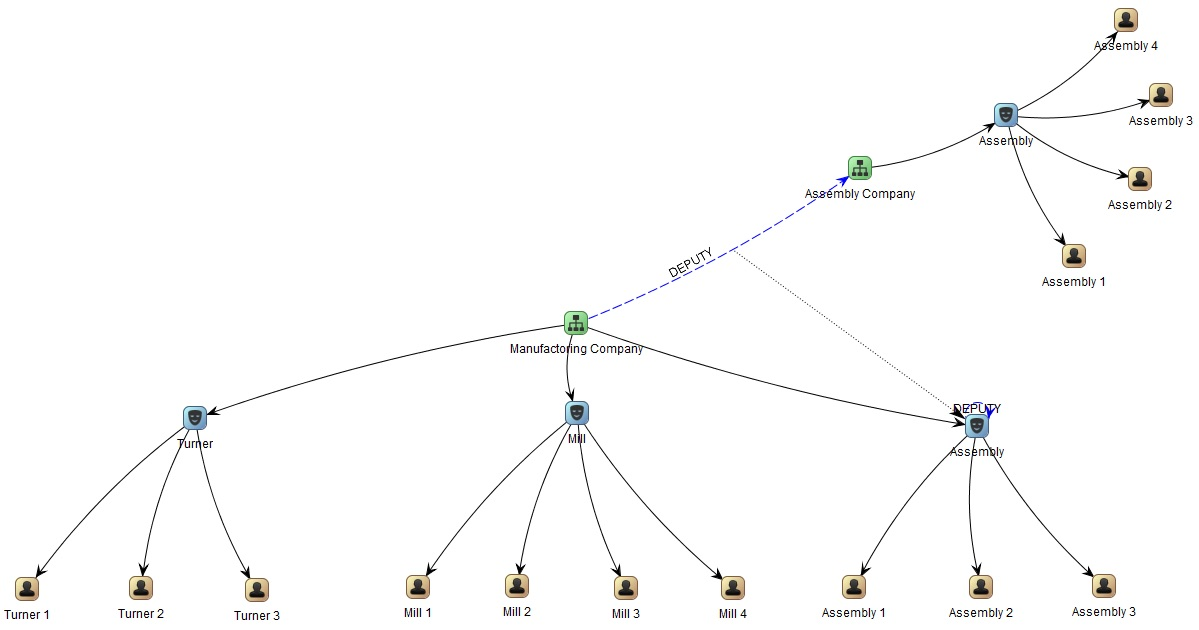
\includegraphics[width=\textwidth]{Figures/orgamodelfed.jpg}
	\caption{Federation between Partner Companies}
	\label{fig:federation}
\end{figure*}

Figure \ref{fig:federation} depicts an excerpt of the organizational model of a manufacturing company producing wooden chairs. The model encompasses the internal organizational unit \emph{Manufacturing Company} with the subordinate internal functional units \emph{Turner}, \emph{Mill} and \emph{Assembly}. The internal resources \emph{Turner 1} to \emph{Turner 3} are related to \emph{Turner}, \emph{Mill 1} to \emph{Mill 4} belong to \emph{Mill} and \emph{Assembly 1} to \emph{Assembly 4} are part of the internal functional unit \emph{Assembly}. 

The properties and capabilities of the elements of the organization can be described using attributes. In our example, the maximum length of a workpiece to be processed and the shape of a workpiece on the machines is of interest.
Table \ref{tab:intagents}  describes an excerpt of attributes in conjunction with their values. 

%The table \ref{tab:intagents} depicts attribute-value pairs of internal automatic resources of the \emph{Manufacturing Company}.
\begin{table}[htb!]
	\centering
	\begin{tabular}{|l||l|l|}
		\hline
		Resource & Attribute & Value \\ 
		\hline
		\hline
		Turner 1 & minworkpieceLength & 30 \\
		\hline 
		& maxworkpieceLength & 50\\
		\hline
		& workpieceKind & octagonal\\
		\hline
		&...&...\\
		\hline
		Turner 2 & minworkpieceLength & 35\\
		\hline
		& maxworkpieceLength & 40\\
		\hline
		& workpieceKind & octagonal\\
		\hline
		&...&...\\
		\hline
		Turner 3&minworkpieceLength & 40 \\
		\hline
		& maxworkpieceLength & 50\\
		\hline
		& workpieceKind & square\\
		\hline		
		&...&...\\
		\hline
		Mill 1& maxLength & 100cm \\
		\hline
		& maxWidth & 100cm\\
		\hline
		& maxHeight & 20 cm\\
		\hline
		Mill 2& .... & ... \\
		\hline
		Assembly1 & Type & 304456\\
		\hline
		& ... & ...\\
		\hline
		Assembly2(PC) & Type & 304456\\
		\hline
		& ... & ...\\
		\hline
	%	&...&...\\
	%	\hline
	%	Mill 3& & \\
	%	\hline
	%	&...&...\\
	%	\hline
	%	Mill 4& & \\
	%	\hline
	%	&...&...\\
	%	\hline
	%	Assembly 1& & \\
	%	\hline
	%	&...&...\\
	%	\hline
	%	Assembly 2& & \\
	%	\hline
	%	&...&...\\
	%	\hline
	%	Assembly 3& & \\
	%	\hline
	%	&...&...\\
	%	\hline
	\end{tabular} 
	\caption{Attributes of Resources} 
	\label{tab:intagents}
\end{table}

Looking at the relationships there exists an external partner company (assembly company) that can take over assembly tasks on load peaks
\footnote{The automated propagation of model elements (entities, relations and attributes) to partner organizations is described in \cite{Lawall2014a}.}. The federation between the manufacturing company and the assembly company extends the aforementioned organizational model. The external organizational unit \emph{Assembly Company} encompasses the external functional unit \emph{Assembly} in conjunction with the external resources \emph{Assembly 1} to \emph{Assembly 4}. 

%So a partner company can act as a proxy. This substitution is described in detail using attributes and hyperedges. For a deeper understanding, please refer to the article \cite{Lawall2014a}.  

Finding the correct agent for a specific task is done by resolving an organzational language expression that is defined in the subject specification.
The expression can reference entities, relations and/or attributes. 
Suppose a production agent wants to have 64 chair legs manufactured for the production of a batch of chairs of type 304456. He first looks in the master data record to see what specifications the legs must have. He finds a length of 40 cm and octagonal shape. He can use these two specifications to find a suitable machine. The expression looks like this:\\

\texttt{(Turner)(Manufacturing Company). ATT.(minworkpieceLength $\leq$ "40" AND maxworkpieceLength $\geq$ AND workpieceKind = "octagonal")}\\

This means the production agent is looking for an agent of type "`turner"' that is able to produce workpieces with length 40cm and an octogonal form.The
search is local to the manufacturing company. In our example, turning machines 1 and 2 are eligible for the production step.
Finding a production resource to manufacture the 64 seats and backrests works on the same principle. Now the chairs still have to be assembled. The agent finds a suitable assembly unit with the following query:\\

\texttt{ (Assembly)(*).ATT.\\(Model $=$ "304456"))} \\
 
The asterisk means that substitutions are also permitted for this request. Thus, the company's own production facility (Assembly 1) as well as the machine of the partner company (Assembly 2) can be found. Depending on the degree of workload of the resources, the agent decides whether he then locks the order on his own machine or the machine of the partner company. \\

Similar to production resources, software products, actuators or sensors can be modelled and managed according to the same principle. 


%\section{IT-Systems and Software}

% Review Christian Stary January 2020

\chapter{Aspects for further standardisation activities}

\todo{CS: Hochkommas und - im pdf falsch gedruckt.}

In this chapterr various aspects of the subject oriented modelling and programming concept are outlined. These aspects have already been published on different conferences. The following sections are based on these publications. CS: They contain original text parts and thus, the conclusions need to be aligned to the standardization effor, as tried for Fog Computing.
The concepts described in theses sections will be part of future standardisation activities.
The following sections are based on following publications:\\
\begin{list}{-}
	\item Subjects and Shared Input Pools: \cite{article:SharedInputPool}
	\item Subject-Phase Model based process specifications \cite{article:SubjectPhase}
	\item Hierarchies in Communication Oriented Business Process Models: \cite{article:Subject-hierarchies}
	\item Business Activity Monitoring for S-BPM: \cite{article:SubProcessMon}
	\item Subject Oriented Project Management: \cite{article:Subject-Oriented-Project-Management}
	\item Subject-oriented Fog Computing: \cite{article:FogComp}
	\item Activity based Costing \cite{article:SBPMCosting}
\end{list}

\section{Subjects and Shared Input Pools}

Shared input pools have the same structure like subject-specific ones, and thus, the same properties like the standard input pool. The only difference is that different subjects can deposit in or remove messages from a shared input pool. Subjects that want to send a message via a shared input pool do not use a subject name as addressee of a message, but the name of a shared input pool instead. In a distributed system several shared input pools for different purposes can be used. Figure 7 shows the slightly changed structure of the traffic management system when operating it with a shared input pool CS: hier fehlt das originäre Beispiel als Bezugspunkt. The subject "Car detection" represents the shared input pool.


\begin{figure}[htbp]
	\centering
	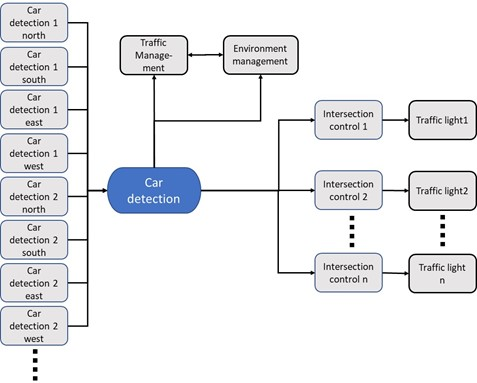
\includegraphics[width=0.9\linewidth]{Figures/Chapter5/figuresshared/SharedInputPoolExample.jpg}
	\caption[Traffic Management System with Shared Input Pool]{Traffic Management System with Shared Input Pool}
	\label{fig:SharedInputPooTraffic}
\end{figure}


Shared input pools make a distributed system more flexible when additional participants or nodes are added. For instance, a third intersection control could be added to the traffic management system without much effort. In this case, only the additional detectors and the components for controlling the intersection have to be complemented and linked to the shared input pool. The extension would have no impact on the behavior of the other subjects and their behavior in that system.
There is one additional attribute for shared input pool: It defines whether a message will be removed from the input pool once a message has been picked up by a receiving subject. This mechanism is required, since several subject may need to process a particular message. In addition, it allows keeping historical information in the input pool, in particular for analyzing the content of an input pool independently of the behavior of interacting subjects.
The messages of an input pool can be analyzed with respect to certain patterns of its messages. In order to perform such an analysis, Complex Event Processing (CEP) concepts can be applied. Complex Event Processing can be encapsulated in a subject. A subject of this kind scans the messages of a shared input pool and checks whether patterns of interest can be found. Once such a pattern is identified, a message including the discovered pattern can be sent to other participants, and initiate further activities. Figure 8 shows the traffic management example enriched with subjects processing complex events.
In the example, the subject "CEP pollution analyzer" can analyze the time between cars passing the intersection in a certain time period. It can identify the events "low traffic" or "high traffic" and send it to the subject "Environment management". In case of tunnels, the subject "Environment management" might react to this information in a different way compared to open air settings.


\begin{figure}[htbp]
	\centering
	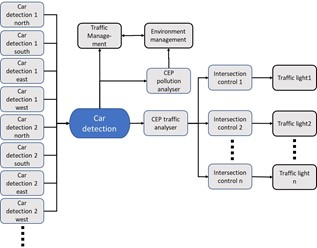
\includegraphics[width=0.9\linewidth]{Figures/Chapter5/figuresshared/SharedInputPoolEvent.jpg}
	\caption[Shared Input Pools and Complex Event Processing]{Shared Input Pools and Complex Event Processing}
	\label{fig:sharedInputPoolEvents}
\end{figure}

\subsection{Implementing Shared Input Pools}
As mentioned earlier, shared data repositories represent a single point of failure of a distributed system. A malfunction of a shared data storage component or device may have a significant impact on the functionality of the whole distributed system. If a subject or a communication line is disturbed, only a small part of a system may be concerned but if a shared data store is down this has an impact on all subjects accessing this input pool.
\\
In addition to this operational problem it must be decided in the course of organizational implementation which organization is held responsible for running and maintaining the system hosting the shared data. Such issues become prominent, if a distributed system is connecting several independent organizations, e.g., different companies in a supply chain. Distributed systems run by independent organizations may also have to deal with several changes dynamically, affecting the data quality and system stability. Even companies can be replaced by other organizations. If only functional subjects are concerned, such a change can be managed without affecting the operation of the entire system: The execution of a subject is just assigned to the new actor. The problem is more serious if a company leaving a distributed system is responsible for running the system with shared data, as other participants of the shared system are affected. Then, a new company still part of the distributed system must take over the responsibility for the shared data. The migration of these data from one company to another can become very cumbersome from the business point of view and from a technological perspective, too.
One way to solve these problems is implementing shared input pools with blockchain technology. A blockchain is an open, distributed ledger that can record transactions efficiently in a verifiable and permanent way. Blockchains allow to achieve the integrity of a collection of data in a distributed peer-to-peer system, whereas the number of the peers is unknown and an unknown number of them are not reliable and trustworthy \cite{book:Blockchainbasics}.
\\
Today, blockchains are mainly used for managing the ownership of money, goods, real estates, etc. Each participant in a distributed system may have a copy of a blockchain. Changes in a blockchain follow a mechanism which manage changes in a consistent way and the change protocol guarantees that any participant will have again a consistent copy after a change. A change of a blockchain means that a new data record is added, and nothing can be removed from a block chain. Adding a new block to a block chain requires some effort from parties involved in a blockchain. This effort is rewarded by adding crypto money to the party when having accomplished the task successfully. These rewards serve as an incentive for the creators of blocks.
\\
Although heavily questioned with respect to effort and gains by practitioners \cite{article:BlockchainUniverse} blockchain technology provides concepts ensuring the trustworthiness of system components. The latter becomes crucial when operating sensitive distributed systems, such as public transportation and healthcare, in particular when event-based data fusion is needed, where nodes of various type (sensor systems, vendor-specific monitoring systems. user devices, household items, etc.) exchange notifications of events and decision-relevant data with each other. In such settings, not only notification mechanisms needs to be streamlined in case of heterogeneity of nodes, but also data source trust is important for further processing and system behavior \cite{article:EventbasedSensor}.
\\
In order to ensure dependable sharing of data, these basic properties of blockchains need to be adapted to the requirements of a shared input pool. Hence, a blockchain-oriented implementation of a shared input pool must meet several requirements:
\begin{enumerate}
	\item Subjects can subscribe for the access to a shared input pool.
	\item Subjects subscribed for an input pool may deposit or read events from that input pool.
	\item Events can be marked as removed from a shared input pool.
	\item Subjects may analyze the content of a blockchain, e.g., when processing complex events.
	\item There must be a mechanism that a block chain can be deleted, once all involved parties agree on that.
\end{enumerate}

Traditionally data received from "things" are not very complex. These data are mainly values as measured by sensors, or binary signals. This may lead to a paradox situation: If such simple data are to be stored in a blockchain, the fee to be paid for adding blocks containing simple data is larger than the value being transferred.
One way to solve the resulting incentive problem is to use permissioned block chains instead of open block chains: Blockchains for dedicated distributed application are not open blockchains like the ones implementing the management of digital currencies.
\\
For the implementation of shared input pools, we suggest managed or permissioned blockchains. For instance, Hyperledger Fabric \cite{article:hyperledger} is an open source implementation of a permissioned blockchain. Unlike to a public permissionless network, the participants are known to each other, rather than staying anonymous and interacting untrusted. It means, while the participants may not fully trust one another, e.g., in case of being competitors in the same industry sector, a network can be operated under a governance model that is built on the extent of trust existing between participants, such as a legal agreement or framework for handling disputes. When building a business process with known participants, such type of a blockchain implementation would be sufficient. Consensus algorithms for permissioned blockchains are faster and do need much less energy than permissionless blockchain networks.
\\
In \cite{article:Blockbench} it is reported that hyperledger fabric is the fastest available permissioned blockchain. The transaction throughput could even be increased from 3,000 to 20,000 transactions per second \cite{article:hyperledgerfabric}.
\\
When using Hyperledger to create blockchain networks of that kind, a hyperledger blockchain network provides a technical infrastructure offering ledger and smart contract (chaincode) services to applications. Primarily, smart contracts are used to generate transactions which are subsequently distributed to each peer node in the network where they are immutably recorded on their copy of the ledger. The users of applications can be users of client applications or blockchain network administrators.
\\
Subject add messages to the shared input pool and other subjects want to read these messages. If a shared input pool is implemented as a blockchain it is necessary that the chain code (smart contract in Ethereum) realizing the functions of the shared input pool must interact with the world outside the block chain. In hyper ledger fabric (including Ethereum), this problem is solved by so called oracles. We suggest using the blockchain patterns Oracle and Reverse Oracle as described in \cite{book:Blockchainapplications}. For flexibility reasons we prefer off chain oracles - see figure \ref{fig:sharedblockchain}.



\begin{figure}[htbp]
	\centering
	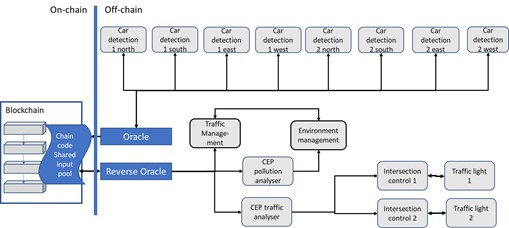
\includegraphics[width=0.9\linewidth]{Figures/Chapter5/figuresshared/Block-Chain.jpg}
	\caption[Utilizing block chain patterns Oracle and Reverse Oracle]{Utilizing block chain patterns Oracle and Reverse Oracle}
	\label{fig:sharedblockchain}
\end{figure}

\subsection {Conclusion}
The more the Internet of Things (IoT) propagates into domain-specific applications, the more stakeholders get involved with respect to business and user requirements. They expect omnipresent use and adaptation on demand. Ensuring robust and semantically correct operation in dynamically networked IoT environments requires tools and development methods to handle complex patterns of interactions due to the different components and capabilities of actors.\\
These patterns refer to the (reactive) flow of control and correct exchange of data. We have proposed an integrated approach based on subject-oriented process models. These role-specific representations allow behavior abstractions on various levels of granularity and can be enriched with a mechanism for handling complex events and sharing data. The data handling mechanism is bound to exchanging messages and a blackboard-like structure. Its behavior can be implemented through blockchain technologies, in case a single point of failure in system operation should be inhibited. The latter is of crucial importance, once the data exchange between IoT-system elements should be trustworthy and traceable.\\
The presented approach should facilitate transparent development and stakeholder understanding of (complex) IoT systems in dynamic settings, due to the implementation-independent representation on a mainly diagrammatic level based on a minimalistic notation, stemming from subject-oriented modeling. Abstractions and decomposition into IoT system components encapsulate behavior. The overall behavior of an IoT system is determined by a set of interactions that integrates the control flow with data exchange patterns from a semantic process perspective. Application design can be understood as top-down approach with the functionality specific to the IoT application residing on an edge operating system. Platform services implement all functional requirements, and are backed by communication and information processing technologies. Cross-functional issues, such as secure operation, business-relevant standardization, and critical event handling can be explicated on an implementation-independent level due to the semantic process representation scheme. The resulting models are executable and thus, can be adapted dynamically.


\subsection{Future Work}
Due to the novel conceptual integration addressed, several aspects and topics need to be addressed by future research:
\begin{list}{-}{spacing}
\item From an application perspective, the results need to be aligned with novel industry 4.0 concepts (cf. [29]), since there not only existing standards are framed by business processes, but also distributed operation of production-relevant processes and real-time sharing of data.
\item From an implementation perspective, our approach requires a (prototypical) realization of an appropriate block chain mechanism for managing shared input pools meeting all requirements in section 4.
\item From an industry perspective, performance evaluations might lead to reconsider our conceptual findings, e.g., how to manage a shared input pool of a distributed system in real time.
\item Definition of structural semantics in OWL
\item Definition of execution semantics in ASM
\end{list}

\section {Subject-Phase Model based process specifications}

\subsection{Introduction}
There are different stakeholders in business process management (see e.g. in \cite{art:Stakeholder}, \cite{book:Worklow-Mod}, \cite{book:BPM-Handbook2}). The most important ones are the customers interested in the result of a process, managers responsible for processes (often called process owners) and the parties involved in the execution of a process (Providers). The parties involved in the execution of a process (providers) can be represented by subjects (see \cite{book:flei2011}. Subjects represent the active elements in a process which communicate with each other in order to coordinate their work producing the required result of a process. Especially middle management wants to get an overview about the process from the event causing the execution of a corresponding process instance (e.g. subject representing the customer of a process) till the results of a process are delivered to the parties expecting it. In the most abstract way upper management is only interested in Key Performane Indicators expressing the efficiency and effectiveness of a process. May be that the delivery of a process result causes the execution of a succeeding process. These succeeding processes use results of the proceeding process as input.
Middle management is interested in who is involved in a process and what  is their contribution to the process result and what are the cost for each contribution. Managers are not mainly interested in the details how the parties involved in a process execute their tasks, how they communicate with each other in order to coordinate their work and which tools and means they use to do their work. Whereas the parties involved in the execution of a process are exactly interested in these aspects of a process. The parties involved in the execution of a process want to know what work they have to do, in which sequences they have to execute these tasks, including when they have to communicate with whom about what and last but not least which means they use for doing their tasks.
On the one hand processes have to be described precisely enough that the parties involved in a process execution know what they have to do in which situation and on the other hand management is primarily interested in more abstract process attributes like key performance indicators and the structure of a process, depending on the management level.\\

Additionally abstract views on processes are needed if complex process systems have to be defined and a top down approach for describing processes is applied. First designers create an overview of a process system and then this abstract model is refined step by step till a model is created which is good enough for the parties working in a process. In order to define hierarchically most methods and tools for process management use different approaches to solve that problem.
In that article an approach is described which allows to get an overview of the involved parties of a process and what are their major contributions to the result of a process. Pracitcal exeprience show that this approach allows to describe the dynamic os a process on one page and the specification is precisely enough to derive executable workflows.

\subsection{Related Work}
Many approaches exist in order to express hierarchies of processes in business process management. In general three to five levels of process specification are used (e.g. see page 53 in \cite{book:Worklow-Mod}, page 52 in \cite{book:Prozessmgmt-umsetzen}, page 92 in \cite{book:EnterpriseBPM}) These process levels are mainly called process areas, business processes, processes, subprocesses and activities. Sometimes sometimes business processes are classified in kernel processes, and main processes (see \cite{book:EnterpriseBPM} page 87. 
In the following sections the abstraction concepts in the mostly used process modeling approaches are outlined.\\

In the ARIS (see \cite{book:ARIS}, \cite{book:SAPRoadmap},\cite{book:EnterpriseBPM}) ecosystem process chains are used in order to give an overview of a process. A process chain shows the process of a process system and defines the sequence in which these processes in the process system can be executed.  There can be several levels of process chains. This means an element representing a process of a process chain can also contain a process chain and so on.  In the lowest level each element of a process chain contains a Event driven Process Chain (EPC). The event driven process chain contains the activities executed in a process. On EPC level the activities are connected to subjects who have to execute an activity. This means only at the lowest level a manager can see who is involved in the execution of a process. It is possible that an activity in an EPC is not one single activity. It can again be an EPC. These various levels of abstraction are focused on the activities executed in a process.\\

BPMN has pools and swim lanes for describing process structures (see \cite{Standard:BPMN}). A process consists of one or several pools and each pool can consist of one or several swim lanes. It is not allowed to have pools in a pool or swim lanes in a swim lane. Activities are assigned to swim lanes. This means there are three abstraction layers: Pools, Swim Lanes and Activities. Pools and swim lanes are used to structure the activities in a process. An activity can contain a sequence of activities. This activity type is called subprocess. An activity in a subprocess can also be a subprocess and so on. This means on activity level arbitrary levels of subprocess are possible. In subprocesses pools and swim lanes are not allowed. Each activity is assigned to a party executing that activity. This means that a pool or swim lane does not correspond to a certain doer. Each activity in a swim lane can be executed by a different provider.\\

This two ways of abstraction are similar to the abstraction used in control flow charts. Only at the lowest level management can see who is involved in a process. The other way around the parties executing the actions have to scan through all the activity sequences in order to find the actions which they have to execute. 
\\
In this paper I want to show an approach in order to specify processes on different abstraction levels for the major stakeholders: Management and doer or provider. On one page managers and the actors in a process see the structure of a process (people and activities) and they get an overview who has to execute which action when.


\subsection{Subject Phase Matrix (S-PM)}

The features of the subject phase matrix will be demonstrated with an example from a real process management project in a small transport company. Figure \ref{fig:process-arch} shows part of the process architecture of that company. There are three processes which built a process chain. There is the process 'Order'. In that process the order of customer will be checked and the transport will be prepared. In process 'Transport' the goods will be transported and in process 'invoicing' the message 'invoice' is send to the subject 'customer' and its payment is controlled. 

\begin{figure}[hbtp]
	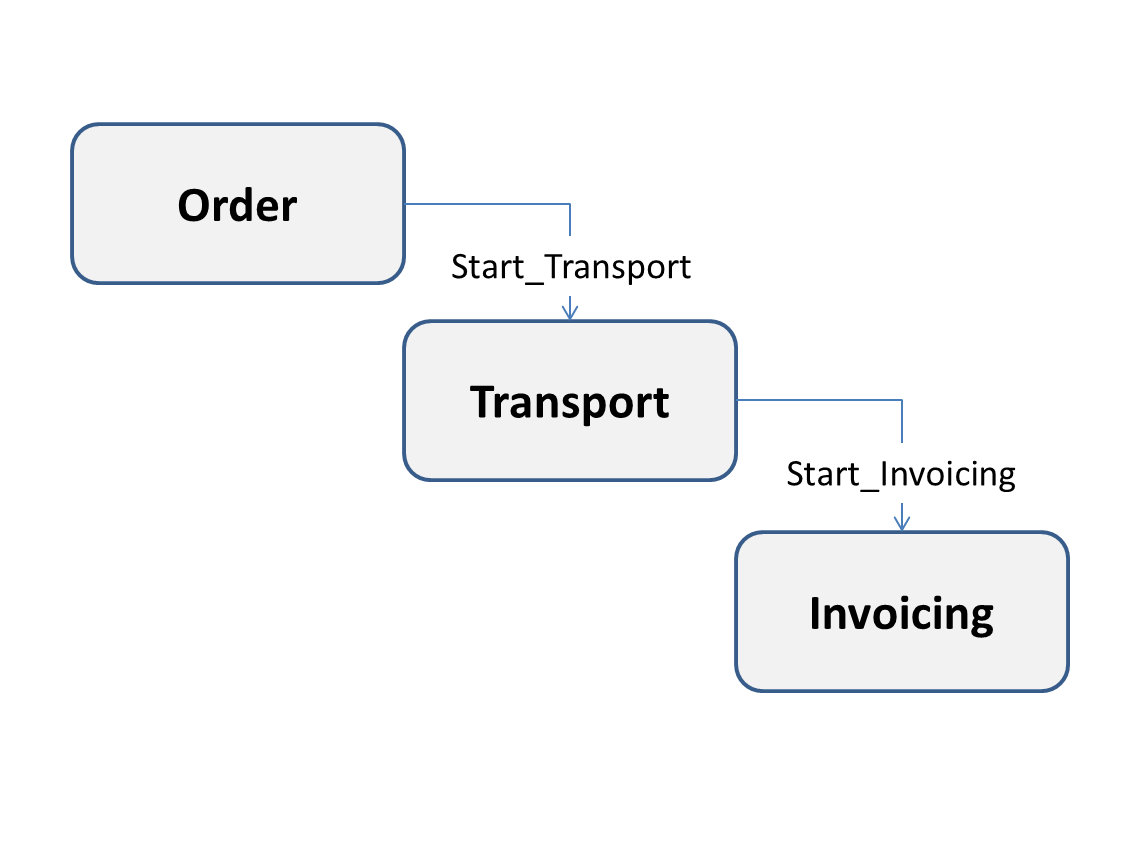
\includegraphics[scale=0.2]{Figures/Chapter5/Subject-Phase/process-architecture.png}
	\caption{Process-architecture}
	\label{fig:process-arch}
\end{figure}

The execution logic of each of these processes is described with a subject-phase matrics (S-PM). The following figure \ref{fig:S-PM-Order} shows the S-PM of the process order.

\begin{figure}[hbtp]
	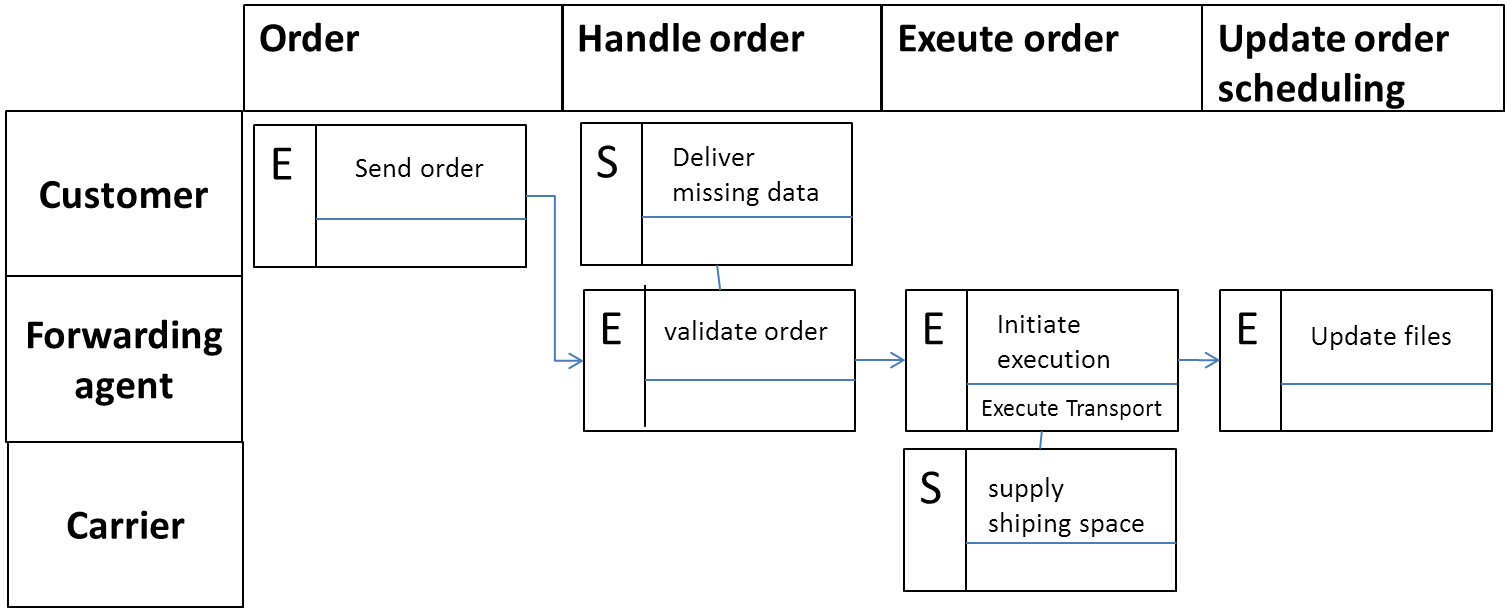
\includegraphics[scale=0.2]{Figures/Chapter5/Subject-Phase/S-PM-process-Ortder.png}
	\caption{S-PM of process 'Order'}
	\label{fig:S-PM-Order}
\end{figure}

A S-PM shows the subjects of a process in the most left column. Subjects  represent the acting parties in a process. Subjects are abstract resources like in S-BPM (see \cite{book:flei2011}). The subjects in Figure \ref{fig:S-PM-Order} are 'customer', 'forwarding agent' and 'carrier'. An S-PM does not show the embedding of a process into an organization. This is a completely separate step as described in \cite{book:flei2011}. This means in that article only the process model is considered. The implementation activities are analog to S-BPM (as described in \cite{book:flei2011}).
Process 'order' shown in \ref{fig:S-PM-Order} has the phases 
\begin{itemize}
	\item order 
	\item handle order
	\item execute order
	\item update scheduling
\end{itemize}
A process is executed from the left to the right, but loops back to proceeding phases are allowed. This means a process starts with the most left phase. In the columns representing the various phases of a process the activities executed in that phase are specified. In a phase it is defined which subject executes which major activity set (marked by an E) and which subjects execute supporting activities (Marked by an S) for the executing subject. In figure \ref{fig:S-PM-Order} the subject 'Customer' executes the activity 'send order' in phase 'order'. In phase 'Handle order' the subject and 'Forwarding agent' are involved. The subject 'Forwarding agent' validates the order and the subject 'Customer' supports in that action. In order to get this support the subject 'Forwarding agent' communicates with the subject 'Customer'. In phase 'Execute order' the subject 'Forwarding agent' is supported by the carrier. In that phase subject 'Forwarding agent' starts the process 'Execute Transport' (Lower part of the rectangle representing the major activity in phase Execute order). If phase 'Execute Order' is finished subject 'Fprwarding Agent' executes in phase 'Update Order Schedulin' the activity 'Update Files'. Figure \ref{fig:S-PM-Execute-Trans} shows the S-PM of process 'Execute Transport' initiated in process 'Order' in phase 'Execute Order' by subject 'Forwarding Agent'.

\begin{figure}[hbtp]
	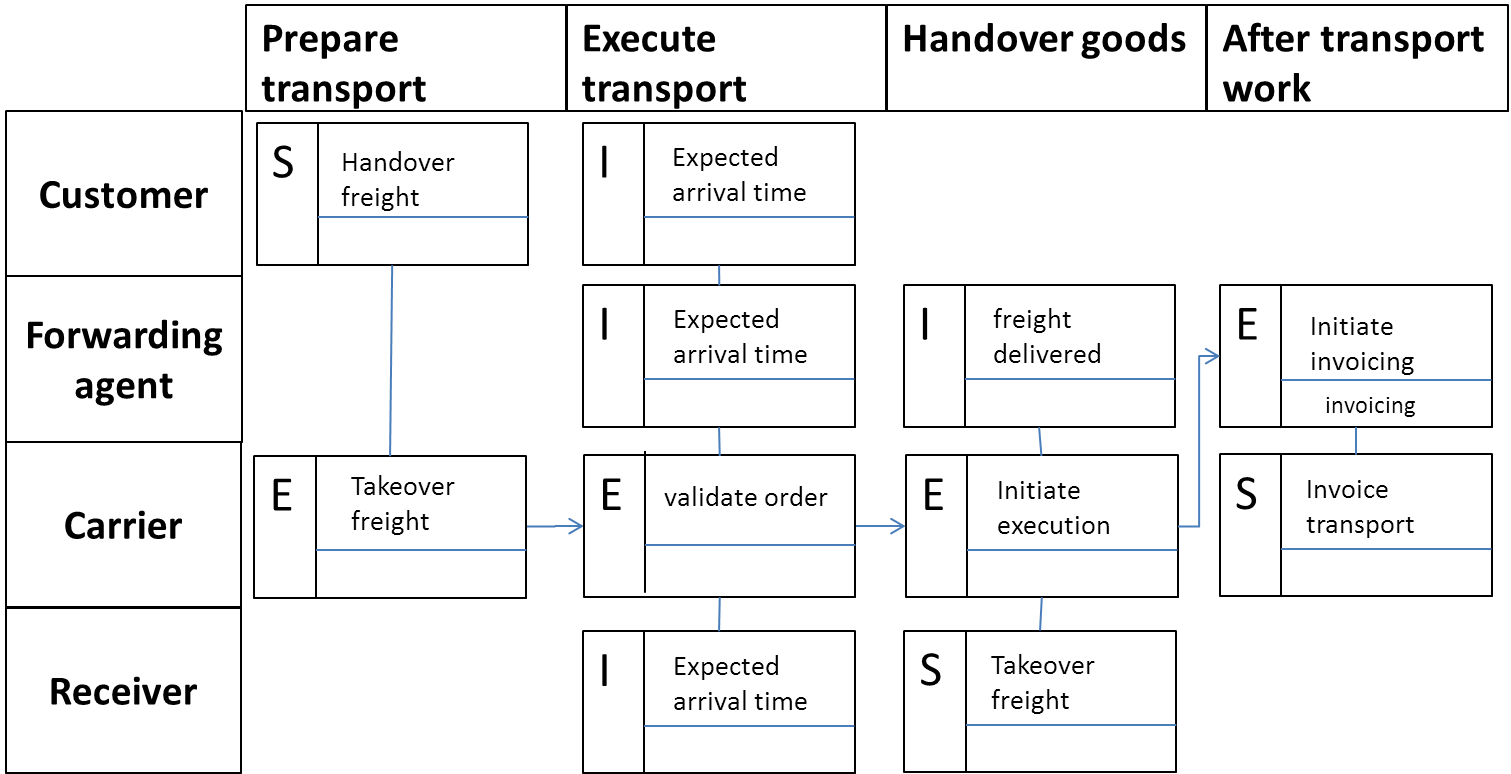
\includegraphics[scale=0.2]{Figures/Chapter5/Subject-Phase/execute-transport.png}
	\caption{S-PM of Process 'Execute Transport'}
	\label{fig:S-PM-Execute-Trans}
\end{figure}


In process 'Execute Transport' some activities are marked with an I. This means that the corresponding subjects are only informed. In phase 'Execute process' subject 'Carrier' informs the subjects 'Customer', 'Forwarding agent' and 'Receiver' about the 'Expected arrival time'.
\\
In the S-PM 'Execute Transport' there is also a subject named 'Customer'. This subject is different from the subject 'Customer' in the S-PM 'Order'. Subject names in a S-PM are valid in the corresponding process. This means subjects in different processes with the same name are different subjects. This does not mean that during the execution of a process (process instance) subjects with the same name in different processes are handled by different persons. Which providers (persons or machines) executes the activities of a subject are defined in the organisational embedding. This is not considered in that paper. This is a task of embedding subjects in an organization (see \cite{book:flei2011}).
\\
S-PMs give an overview about the subjects involved in a process, which activities they execute in which sequence and which relations exists between the various subjects. In many real projects (ISO 9001 projects) more than hundred processes have been specified in that way. It showed up that each process can be structured in phases and processes have between three and six phases only a small number (around 2 percent) have more than six phases. In all cases S-PMs did have more than one page. There has been also the experience that S-PMs are easy to understand also for management and gives the involved parties a first impression what they have to do in a process. In spite of their overview character S-PMs are precise enough that a S-BPM specification can be automatically derived. This will be shown in the following section.

\subsection{Conversion of Subject Phase Matrix to Subject Communication Models}
The conversion of the Subject-Phase-Matrix into Subject Communication Diagrams (SCD) and Subject Behavior Diagrams (SBC) can be done automatically (see \cite{book:flei2011}). In general these SCDs and CBCs are executable without any additionally programming (see \cite{book:flei2011}) but the business objects must be added manually and some internal activities must be specified in more detail. In the following the focus is on the behavior of subjects. Data or business objects are not considered.\\

In order to transform an S-PM into a subject-communication specification we consider the matrix from the perspective of the involved subjects (see figure \ref{fig:S-PM-Execute-Trans}).
\begin{figure}[hbtp]
	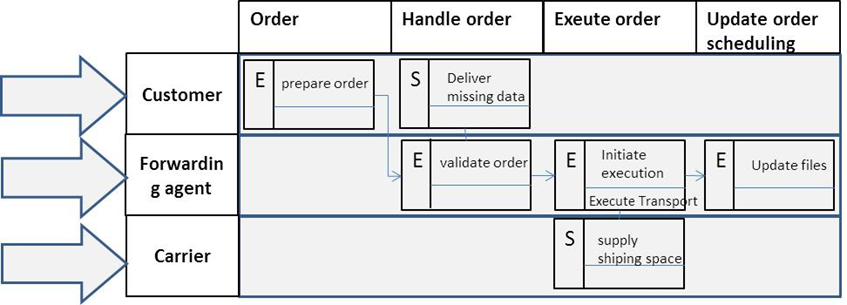
\includegraphics[scale=.4]{Figures/Chapter5/Subject-Phase/s-PM-subject-view.png}
	\caption{S-PM considered from the subject view}
	\label{fig:S-PM-subject-view}
\end{figure}
Each subject in the matrix corresponds to a subject in the subject communication diagram. The names of the subjects in the S-PM are extended with an Id for the process. In our case to each subject name the letters AO are added (AO=Accept Order). A subject sends a message to another subject if in the S-PM the E-action in the succeeding phase is executed by a different subject or the subject needs supports from an other subject. If subjects send a message to the subject executing the E-activity in the succeeding phase the message is named 'E-name-of the-succeeding-phase'. If a subject requests support from another subject the message is named 'S-Name-of-the-phase?'. The receiving subject sends the result of the support request back with a message called 'S-Name-of-the-phase!'. Figure \ref{fig:SCD-Order} shows the communication structure derived from the S-PM shown in figure \ref{fig:S-PM-Order}.
\begin{figure}[hbtp]
	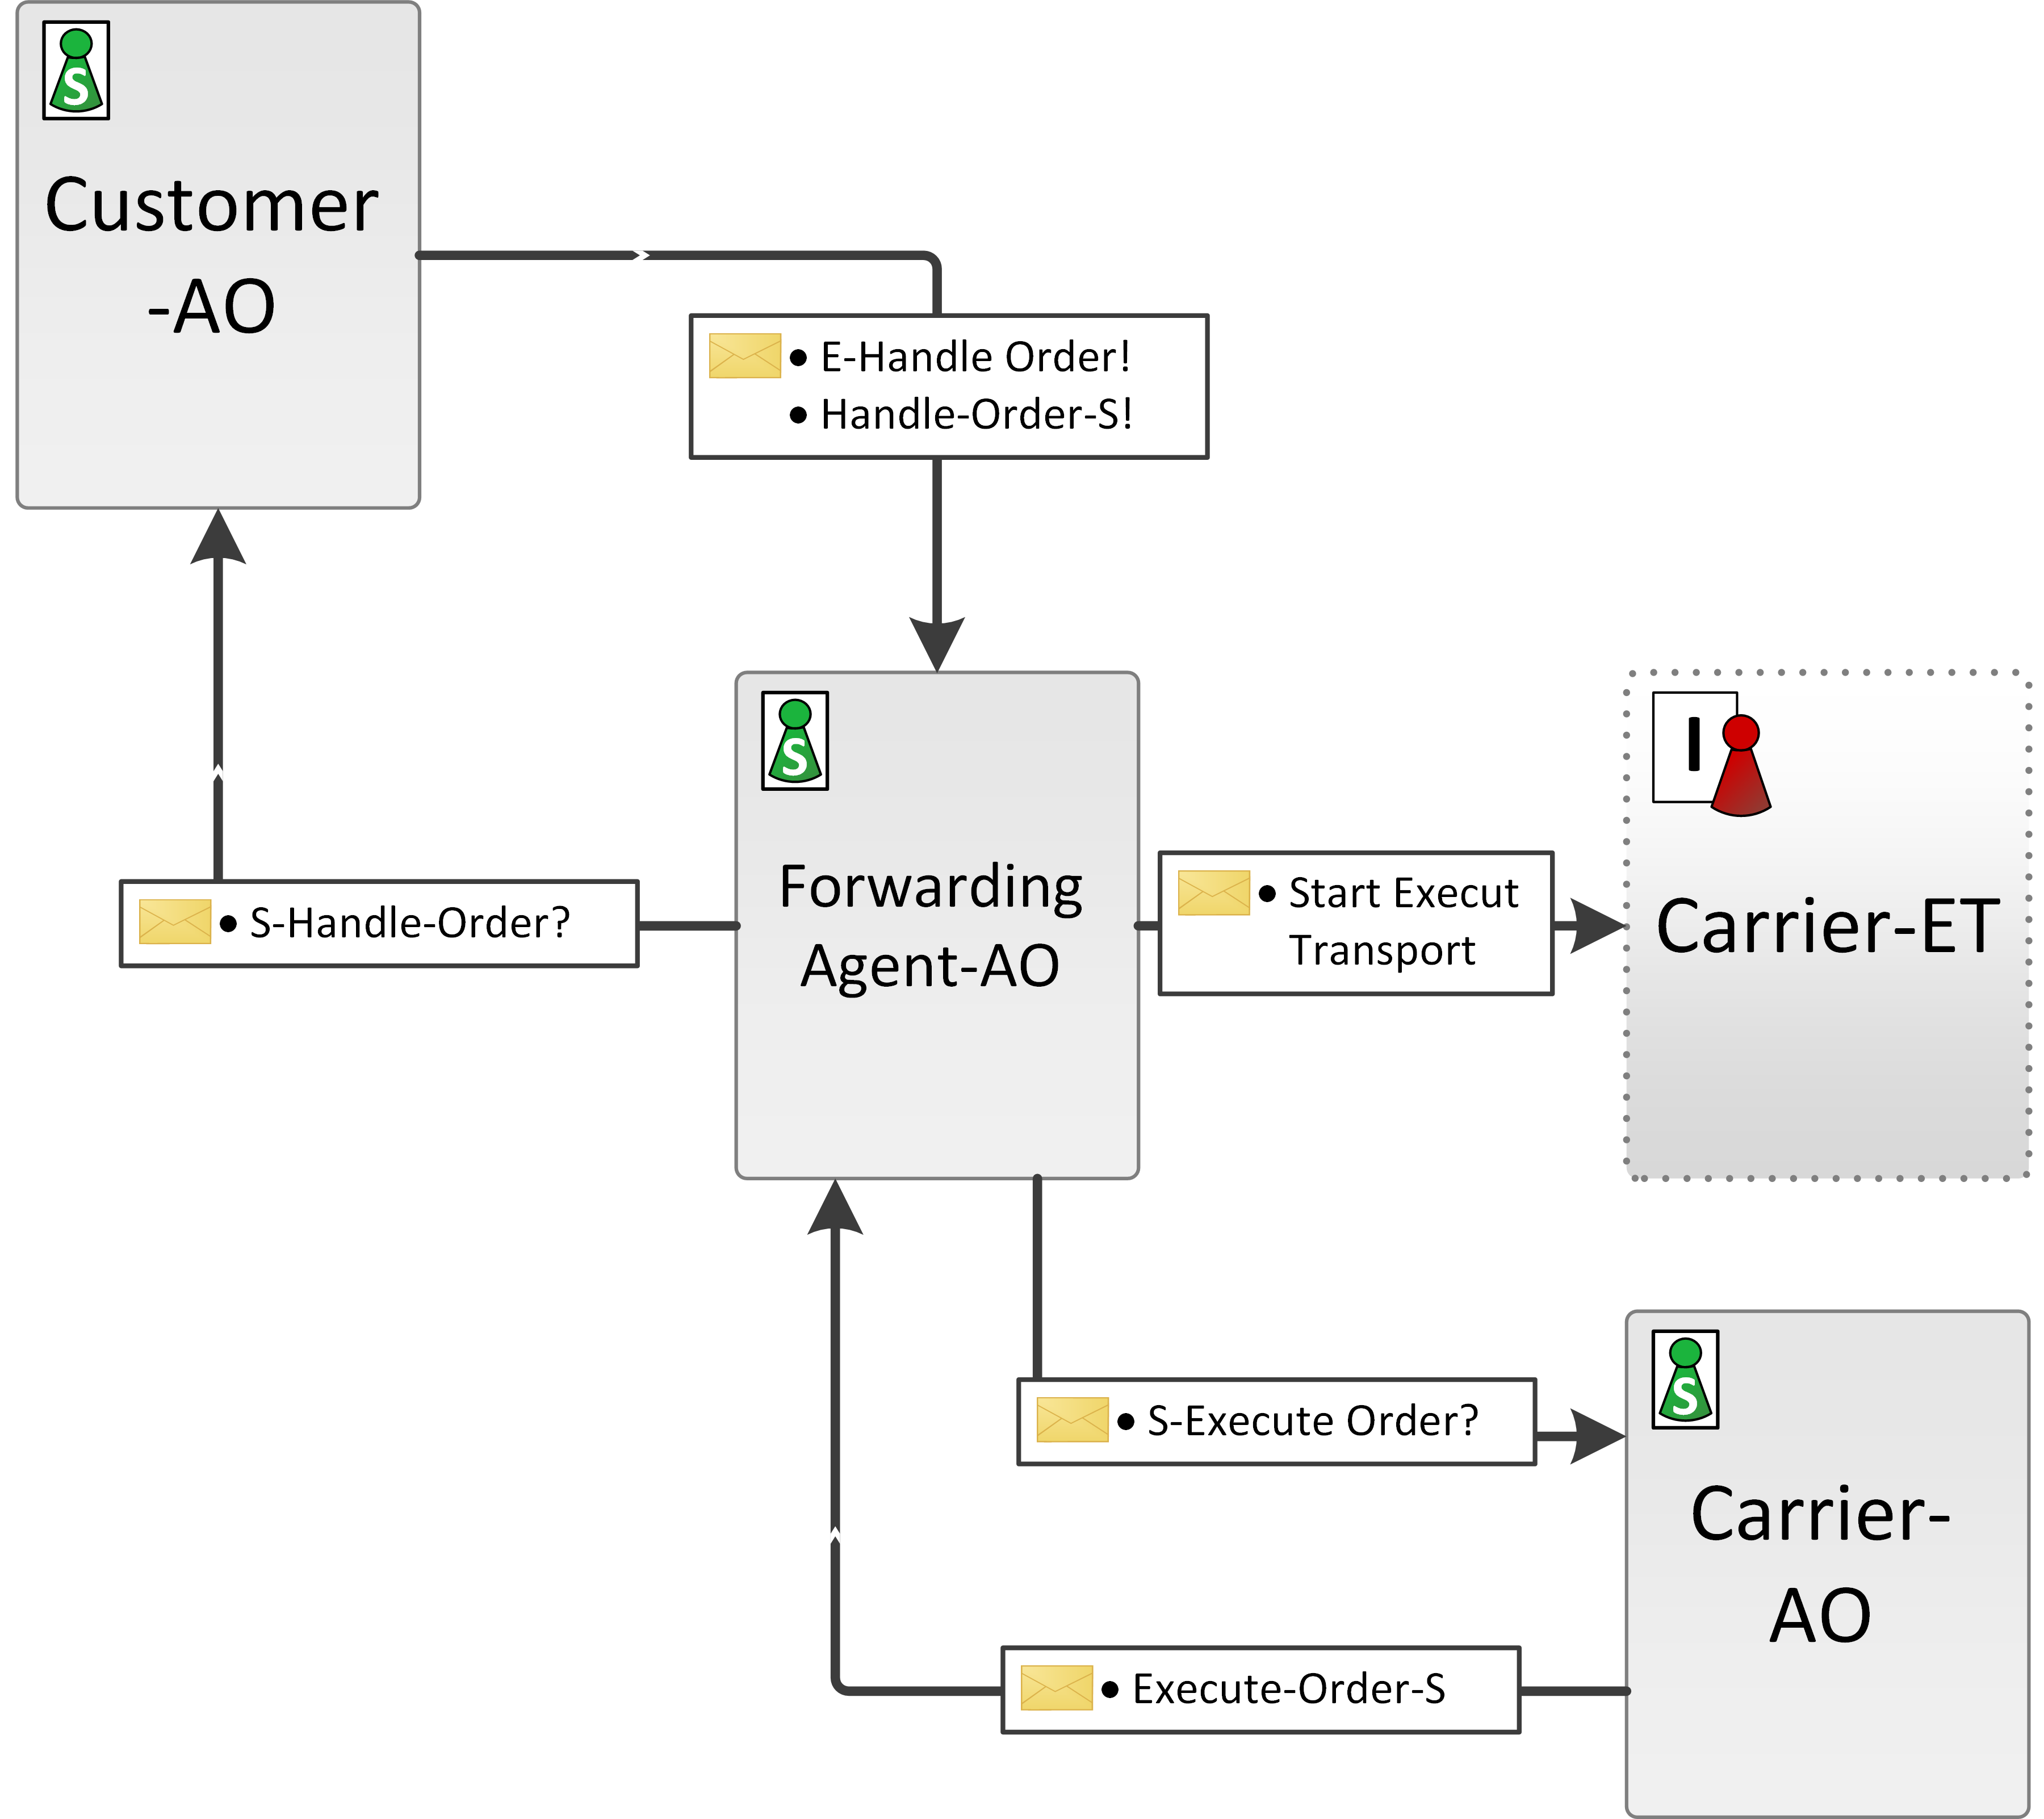
\includegraphics[scale=0.7]{Figures/Chapter5/Subject-Phase/SCD-Order_NEW.png}
	\caption{Subject Communication Diagram of S-PM of Process 'Order'}
	\label{fig:SCD-Order}
\end{figure}
\\
Subject 'Customer-AO' is the start subject. It is the only subject which executes activities in the start phase of the S-PM Order. The succeeding phase 'Handle order' is executed by subject 'Forwarding Agent' therefore subject 'Customer' sends the message 'E-handle-Order' to subject 'Forwarding agent-AO'. This subject executes the activities in phase 'Handle Order' (see figure \ref{fig:S-PM-Order}). \\
Figure \ref{fig:SBD-Customer-AO} shows the behavior of subject 'Customer-AO'. In order to see the relationship between the phases in the S-PM and the activities in the SBD the activities in the SBD belonging to certain phase in the S-PM have frames marked with the phase name.
\begin{figure}[hbtp]
	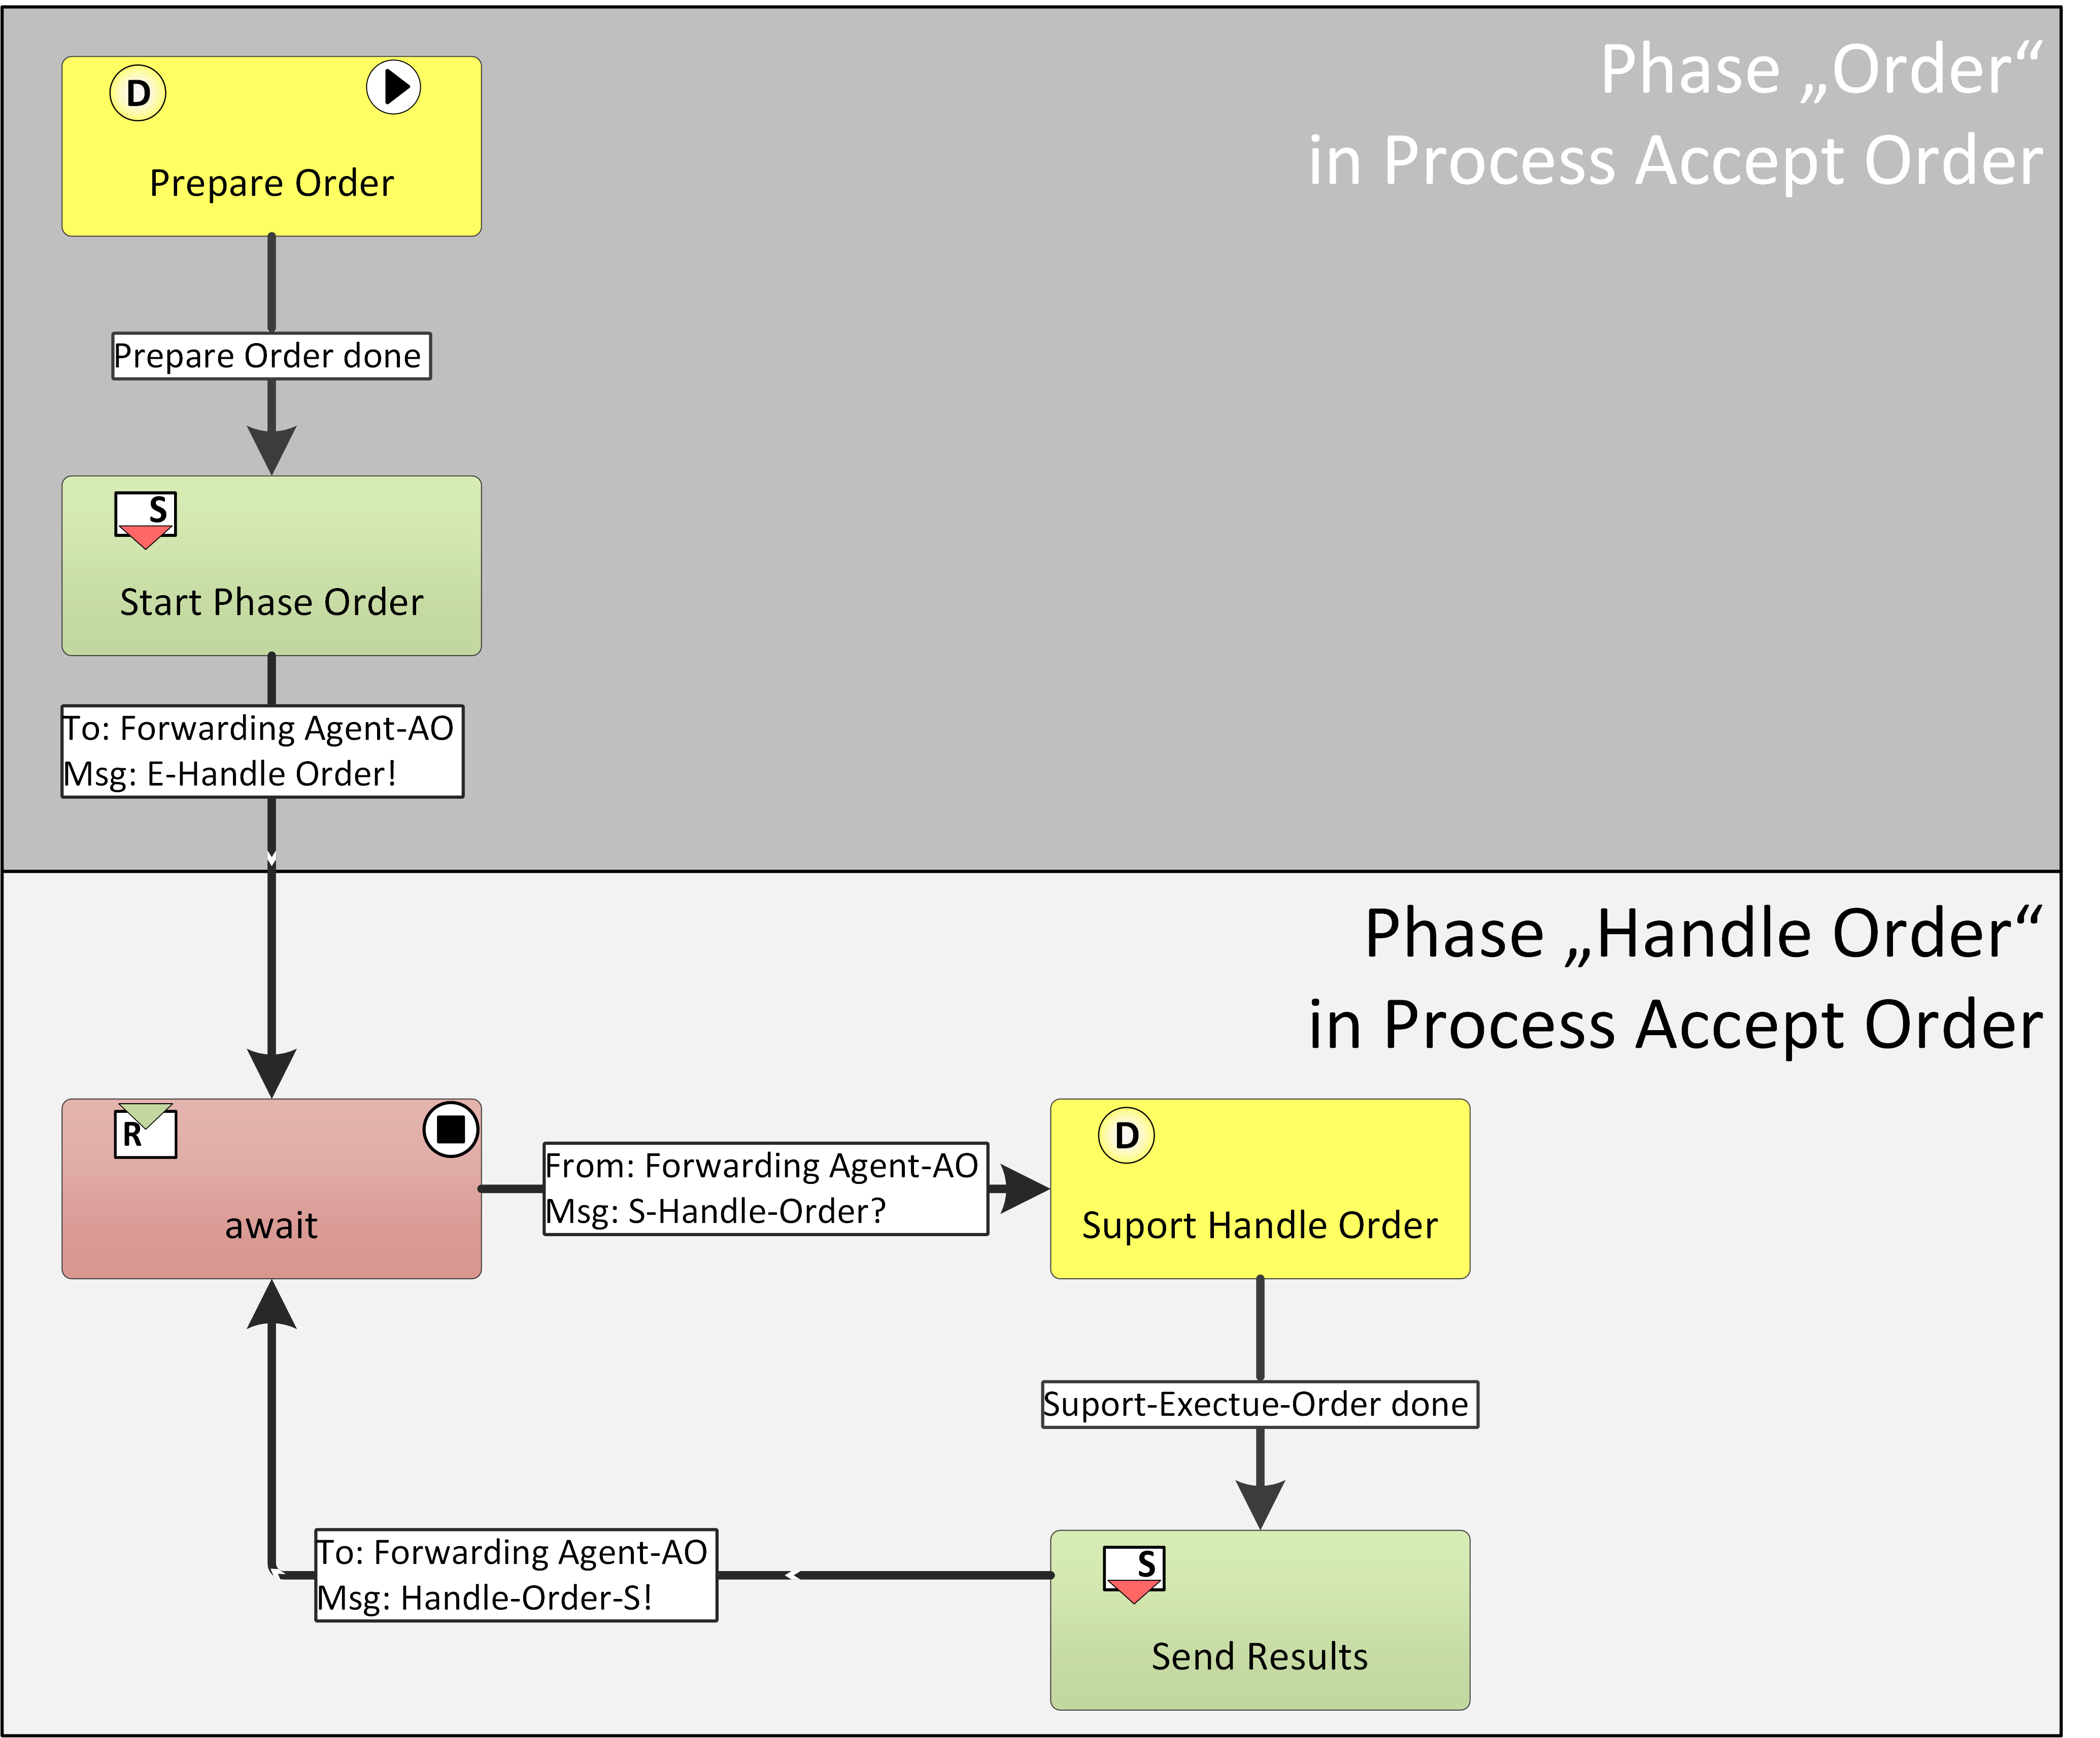
\includegraphics[scale=0.35]{Figures/Chapter5/Subject-Phase/SBD-Customer-AO_NEW.png}
	\caption{SBD of Subject 'Customer-AO'}
	\label{fig:SBD-Customer-AO}
\end{figure}
After the activity 'prepare order' is finished the next phase is started by sending the message 'E-Handle-Order' to the subject 'Forwarding Agent-AO'. Than subject 'Customer-AO' is waiting for the message 'S-Handle-Order?' from subject 'ForwardingAgent-AO'. This is a support request which is sent by subject 'ForwardingAgent-AO' in phase 'Handle order'. The support activity is executed and the result is sent back to subject 'ForwardingAgent-AO'.
The following figure \ref{fig:SBD-ForwardingAGentAO} shows the more complicate behavior of subject 'ForwardingAgent'. 
The subject 'ForwardingAgent-AO' receives the message 'E-Handle-Order' from the subject 'Customer-AO' in phase “Handle Order” in the S-PM. After that message the subject 'ForwardingAgent-AO'  checks whether it need some support from the subject 'Customer-AO'. If support is required a corresponding support request message ('S-Handle-Order?') is sent to the subject 'Customer-AO'. After an answer has been received the subject 'ForwardingAgent-AO' continues its work and checks whether some additional support is required or the activities in that phase can be finished. If that phase is finished the subject 'ForwardingAgent-AO' continues its work in phase 'Execute Order'. Because the subject 'ForwardingAgent-AO' is also the excuting subject for phase 'Execute order' it is not necessary to send an E.message to the executing subject of the succeeding phase. In phase 'execute-orde' the subject 'ForwardingAgent-AO' starts also the process 'Execute-Transport' by sending the message 'E-Start-Execute-Process' to the subject 'Carrier-ET' which is a subject in process 'Execute Transport'.


\begin{figure}[hbtp]
	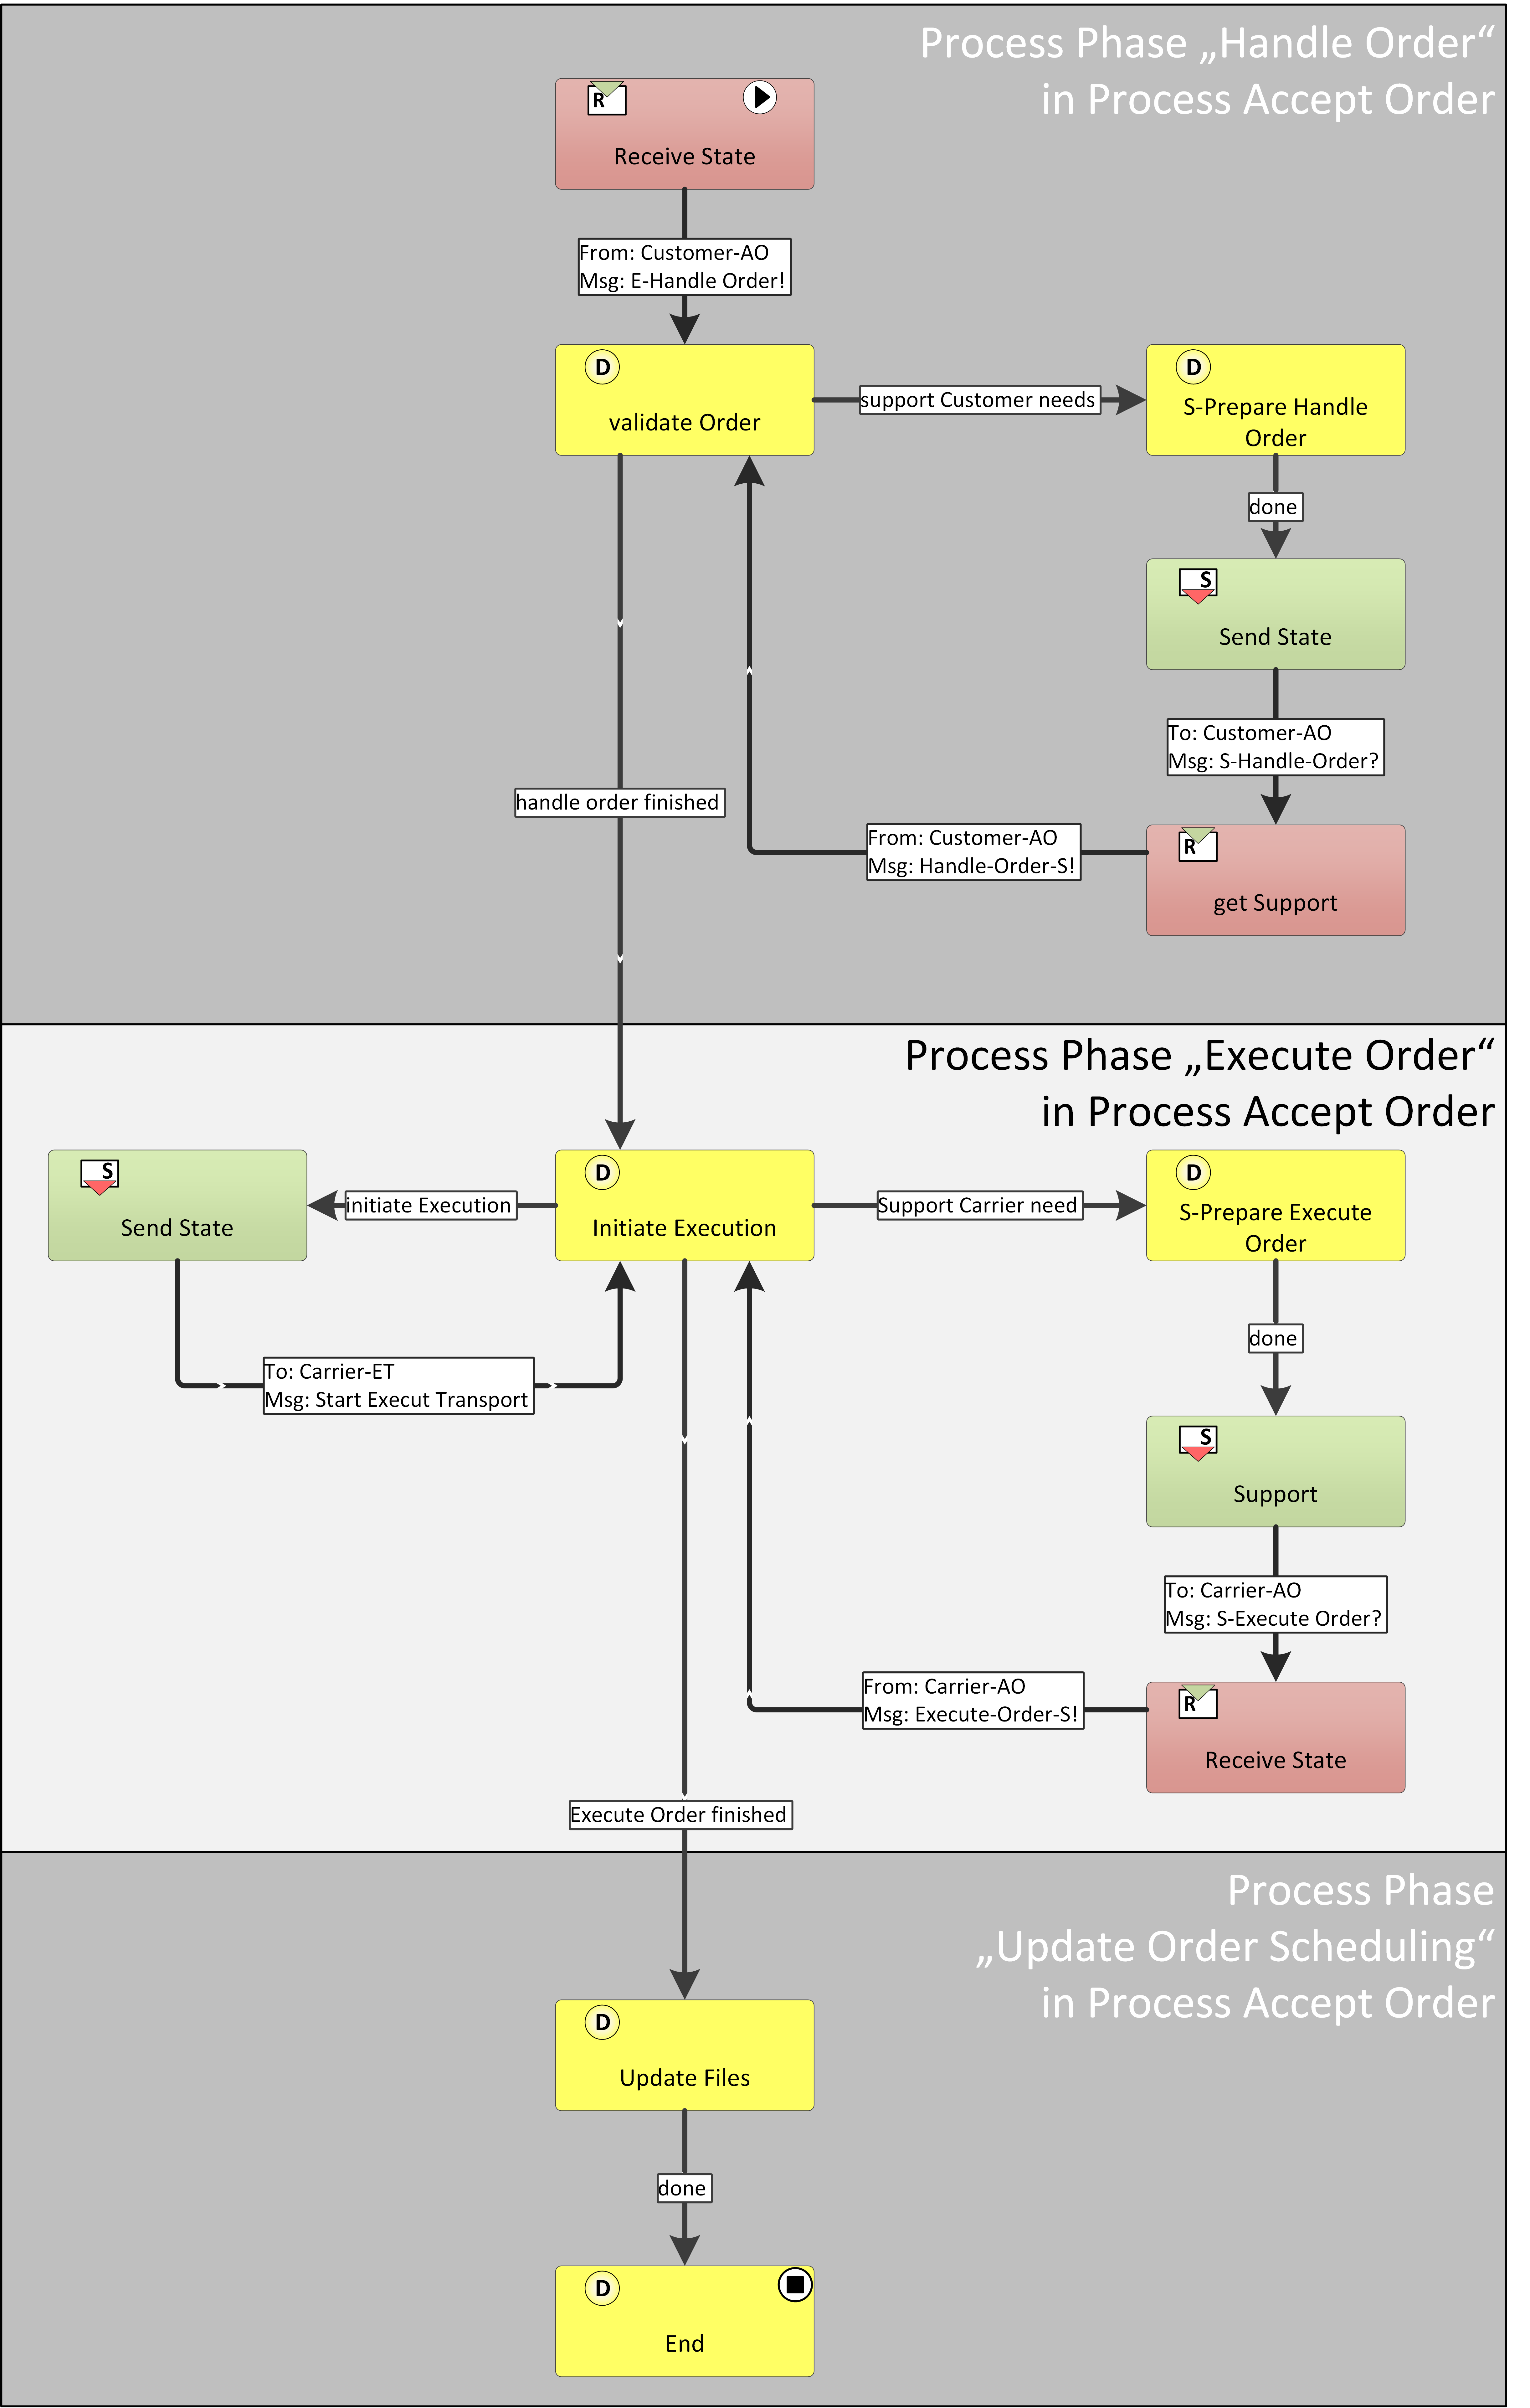
\includegraphics[scale=0.7]{Figures/Chapter5/Subject-Phase/SBD-ForwardingAGentAO_NEW.png}
	\caption{SBD of subject 'Forwarding-Agent' in Process 'Accept Order'}
	\label{fig:SBD-ForwardingAGentAO}
\end{figure}


Figure \ref{fig:CarrierAO} shows the behavior of subject 'Carrier-AO'. In process 'Accept Order' the subject 'Carrier-AO' only supports subject 'ForwardinAgent-AO' in phase 'Execute Order'. This means the subject 'Carrier-AO' receives a support request message 'S-Execute-Order?', excutes the support activities and send the result back to the subject 'ForwardingAgent-AO' by the message 'S-Execute Order!'.

\begin{figure}[hbtp]
	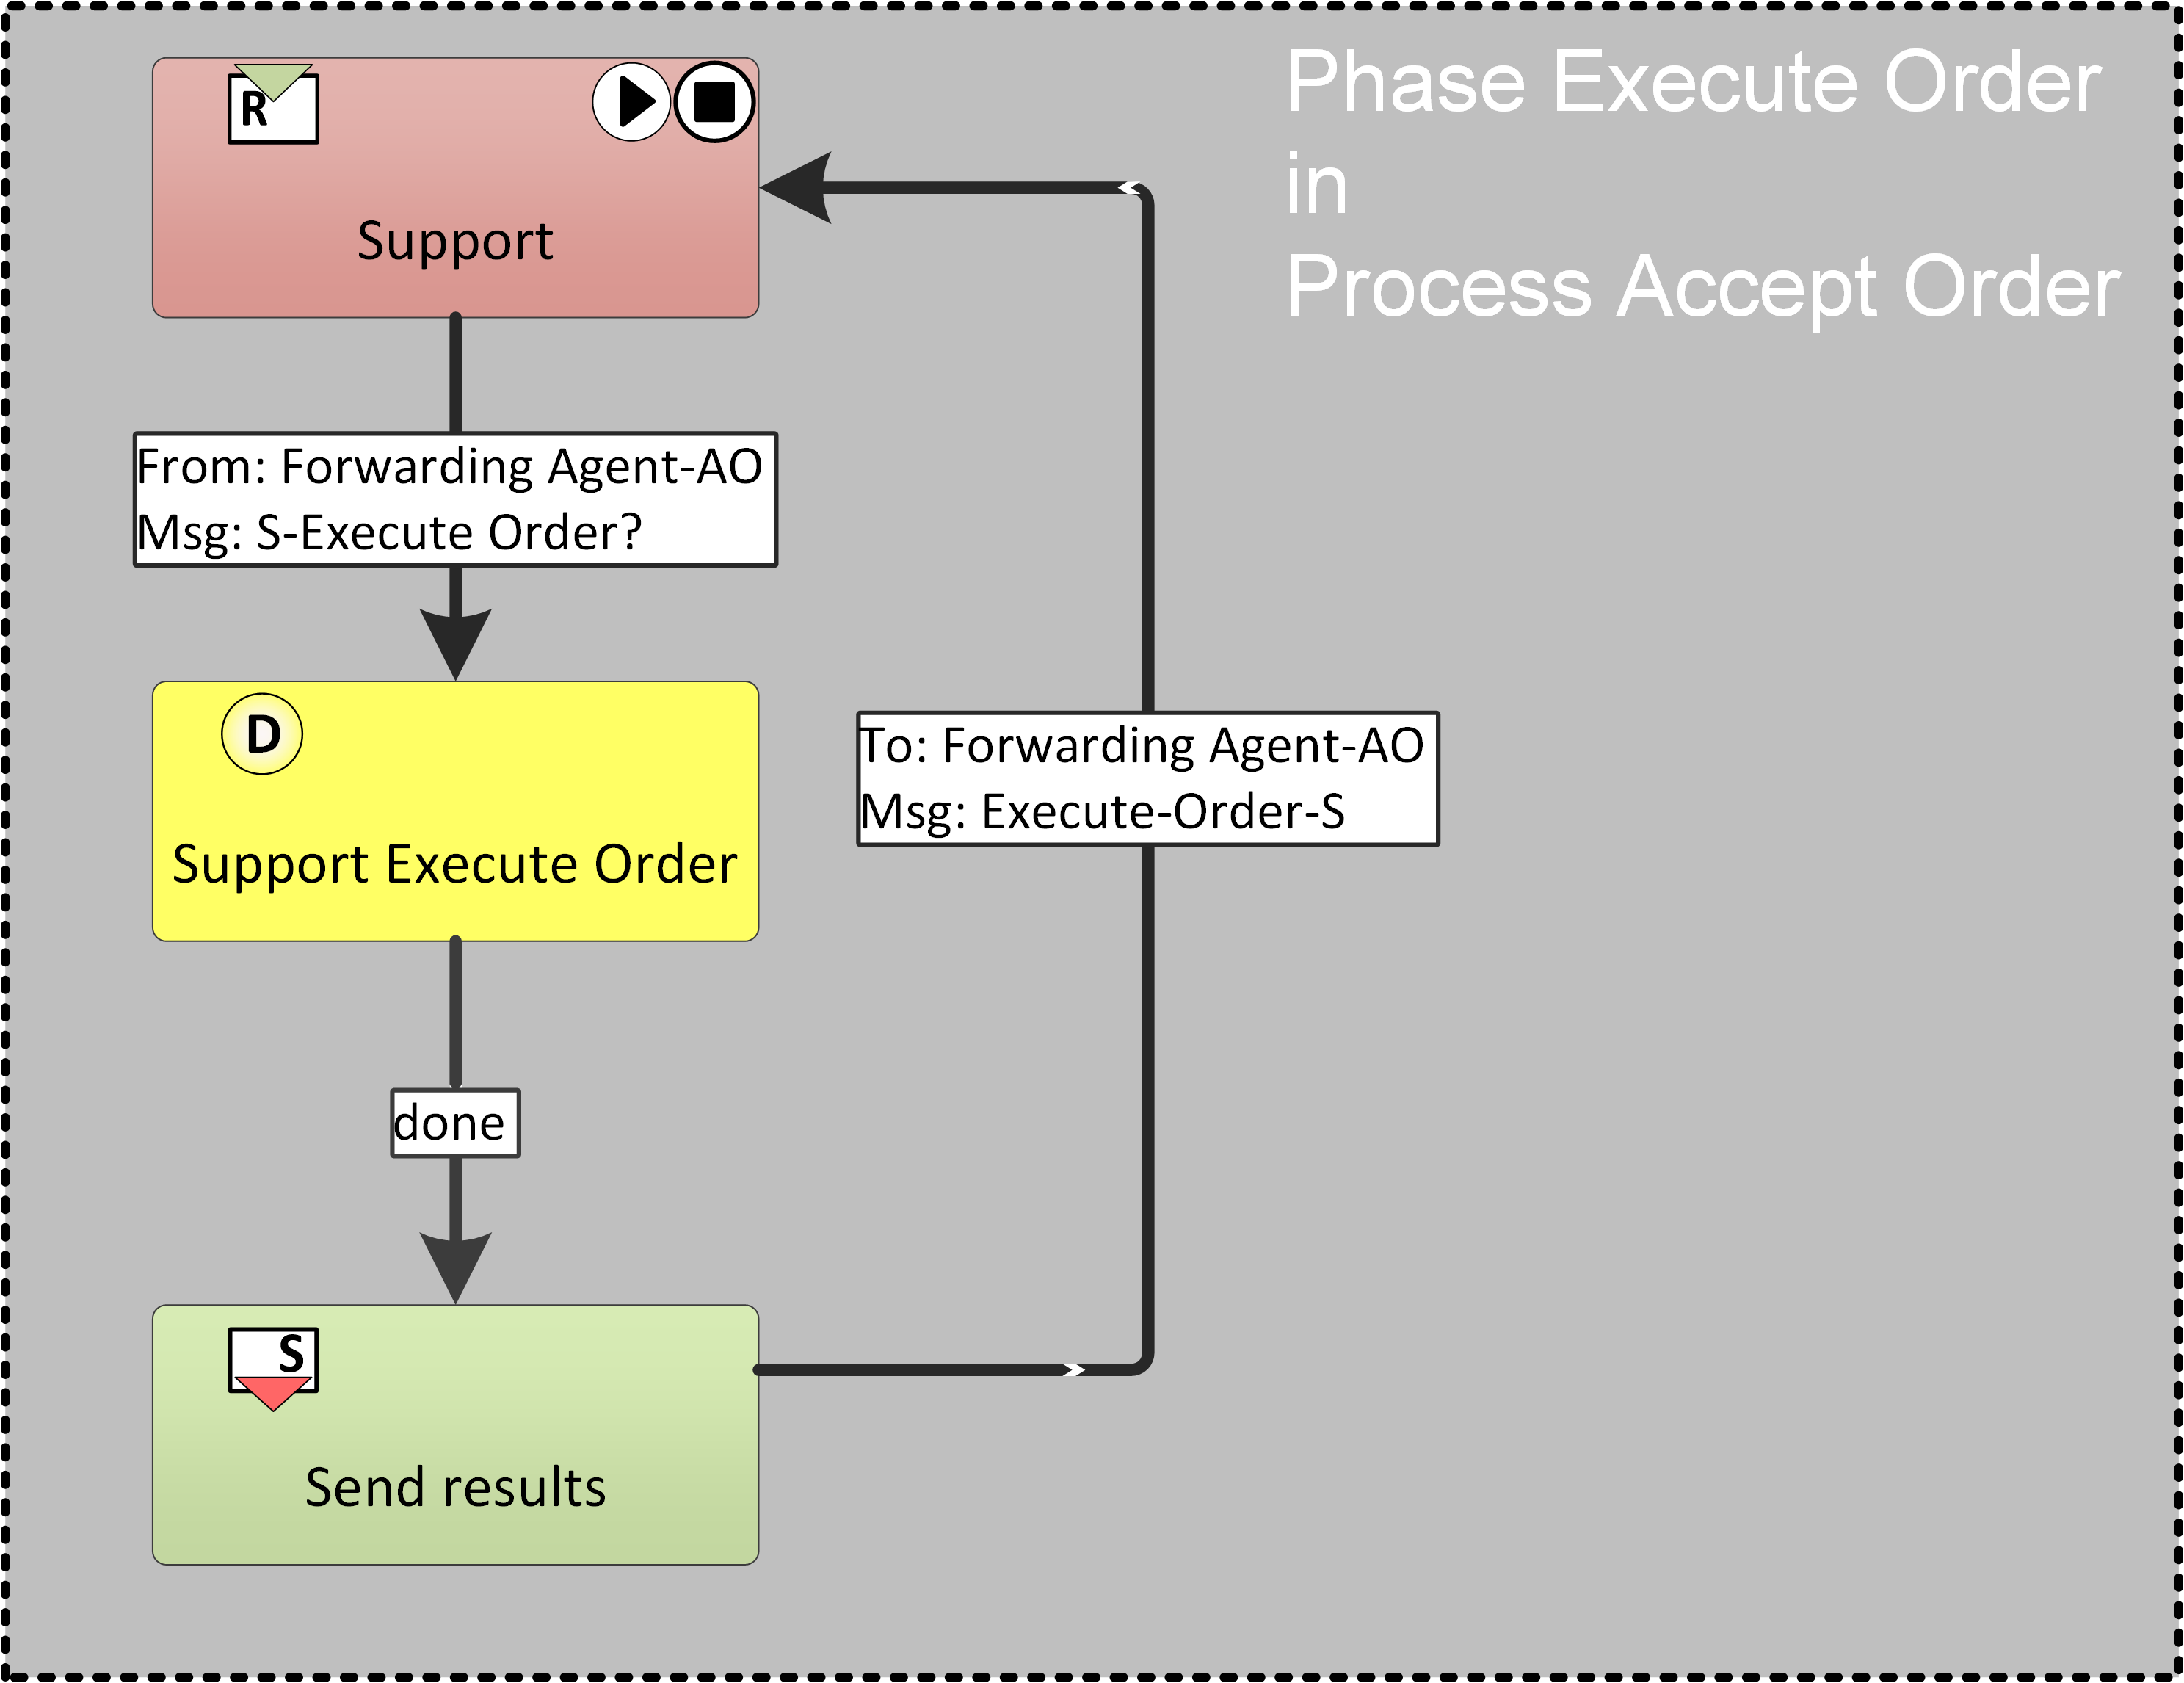
\includegraphics[scale=0.4]{Figures/Chapter5/Subject-Phase/CarrierAO_NEW.png}
	\caption{SBD of subject 'Carrier-AO' in Process 'Accept Order'}
	\label{fig:CarrierAO}
\end{figure}

Figure \ref{fig:SCD-ExecuteTransport} shows the SBD of process 'Execute Process' which is derived from the corresponding S-PM (see \ref{fig:S-PM-Execute-Trans}). The mechanism for getting the communication structure is the same as shown with process 'Accept Order'. The external subject 'ForwardingAgent-AO' represents the starting subject in process 'Accept-Order'.


\begin{figure}[hbtp]
	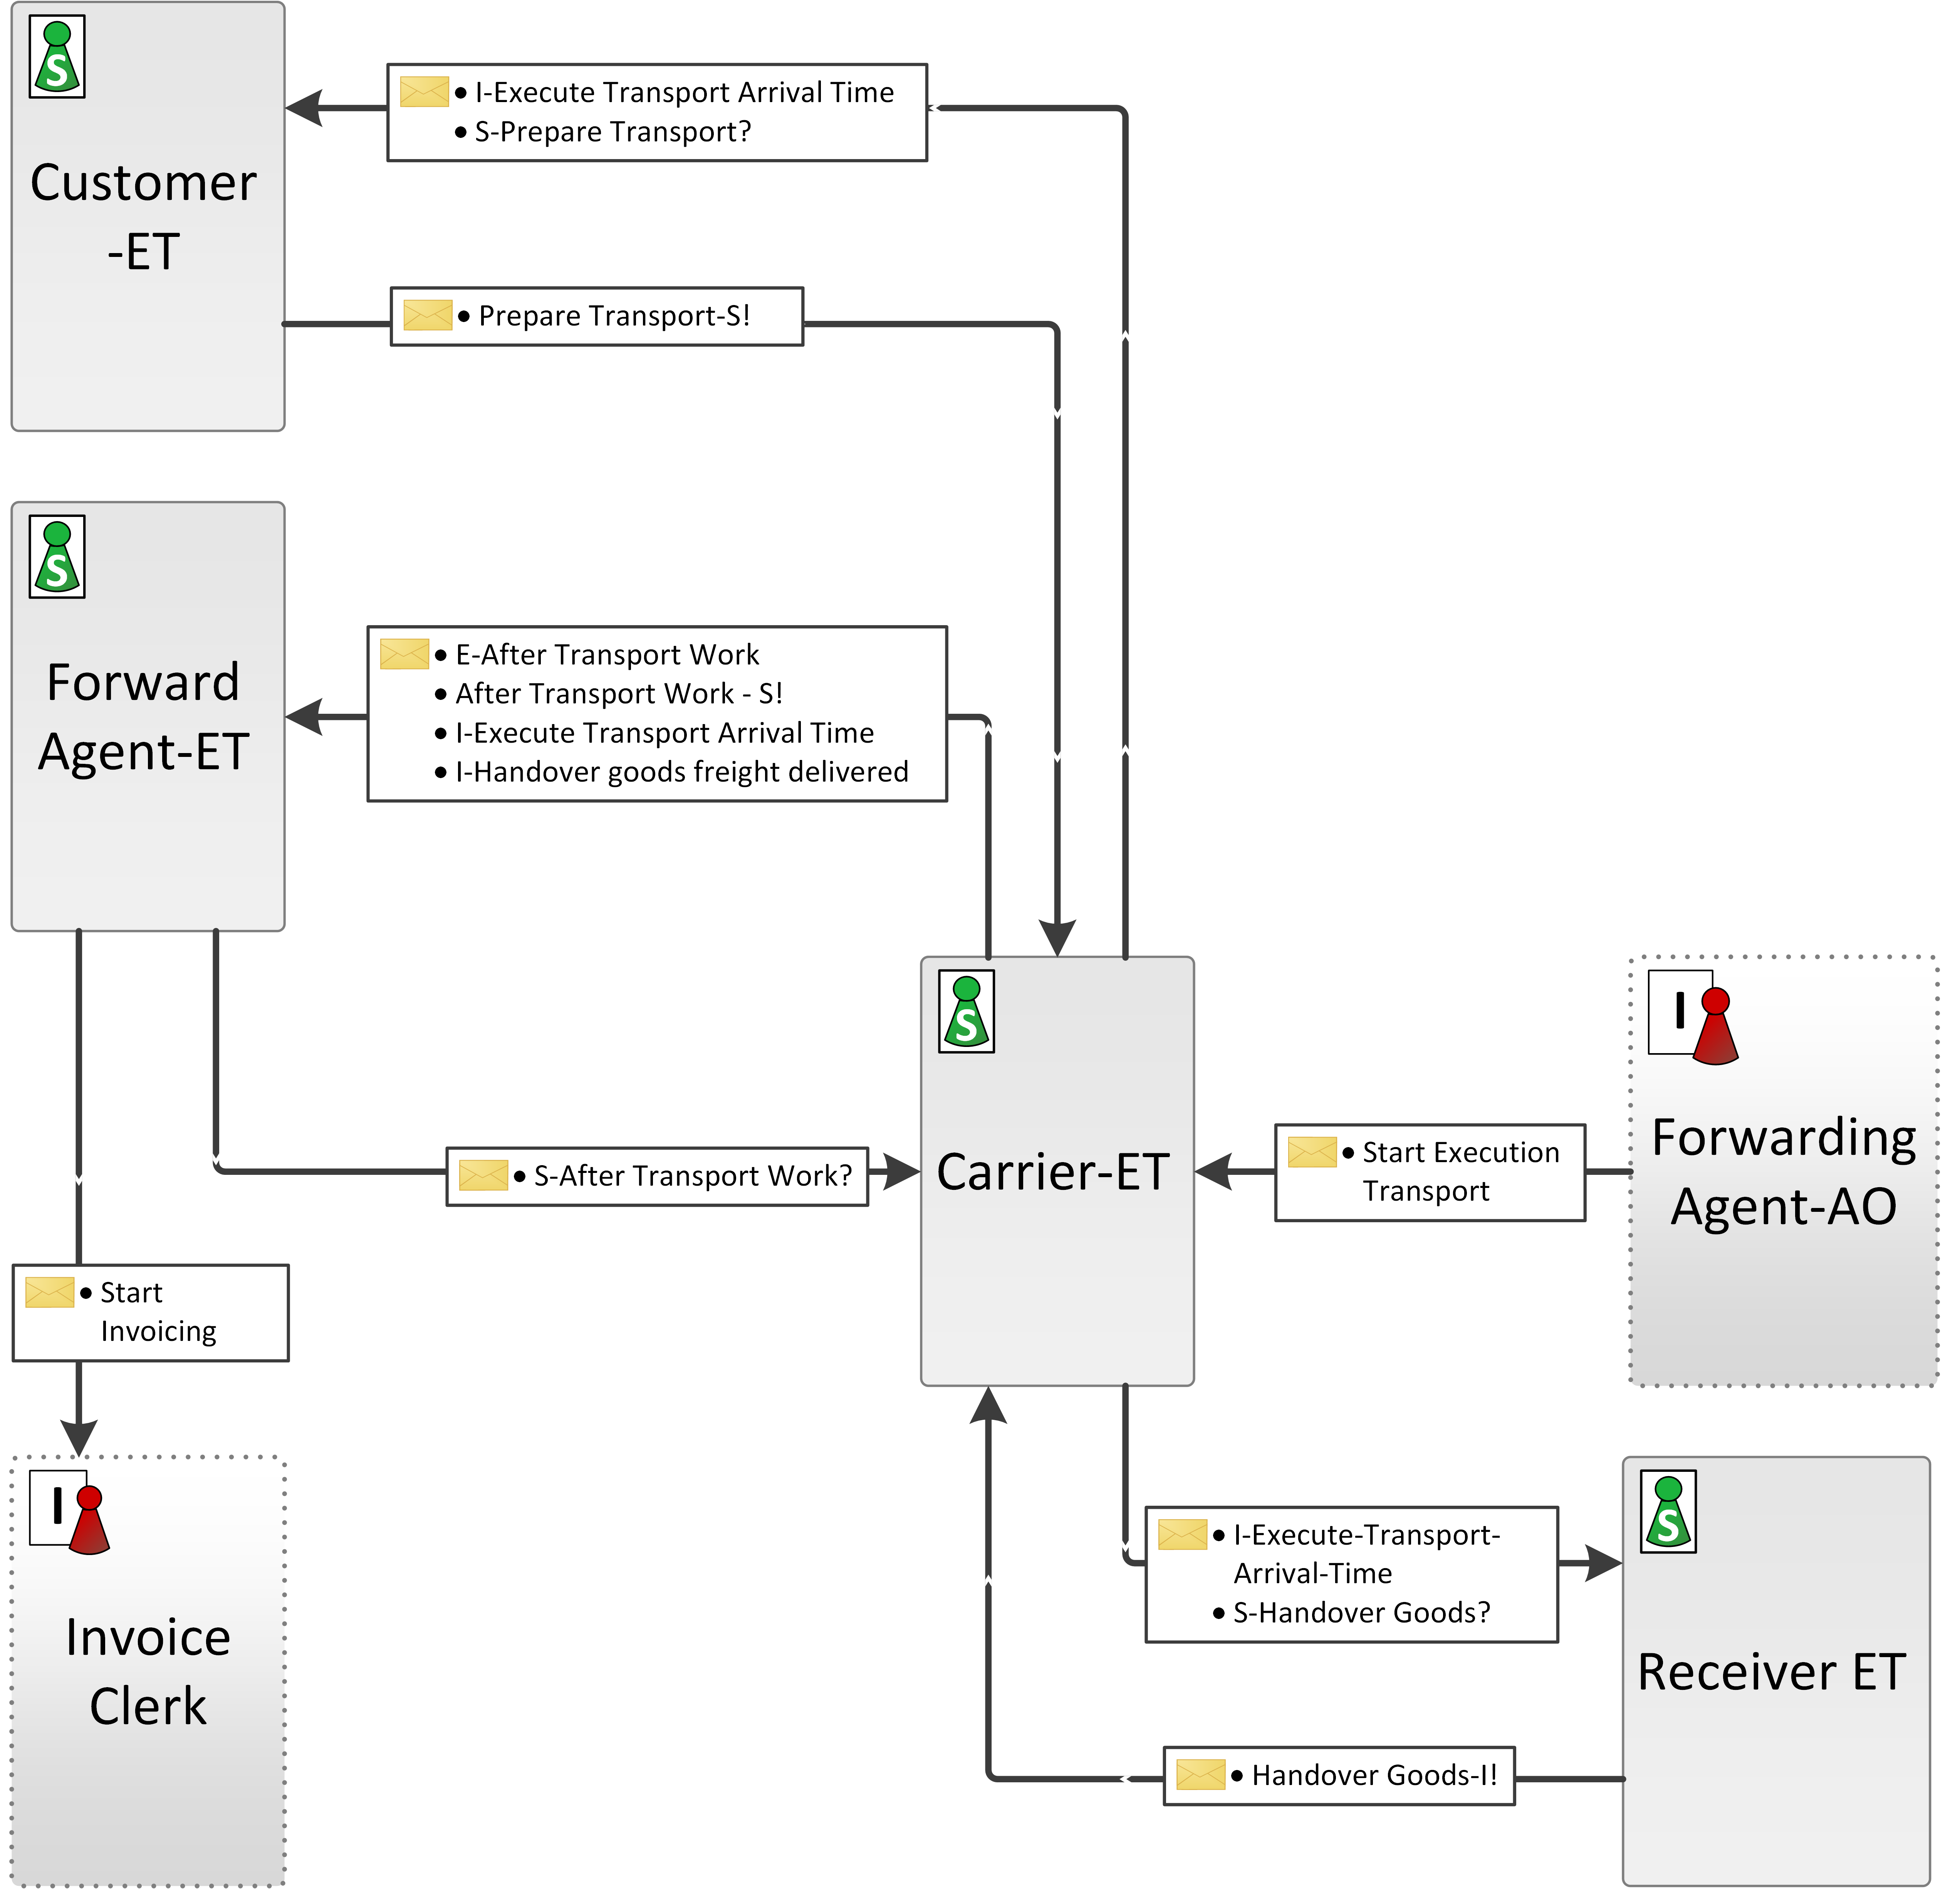
\includegraphics[scale=0.4, angle=90]{Figures/Chapter5/Subject-Phase/SCD-ExecuteTransport_NEW.png}
	\caption{SID of Process 'Execute Transport'}
	\label{fig:SCD-ExecuteTransport}
\end{figure}

Figure \ref{fig:SBD-Carrier-ET} shows the behavior of subject 'Carrier-ET' for the first two phases of the corresponding S-PM shown in Figure \ref{fig:SBD-Carrier-ET}. This subject is different from the subject 'Carrier-AO' but it can be handled by the same person. But this is a decision during the embedding of a process into an organizational structure (see \cite{book:flei2011}).


\begin{figure}[hbtp]
	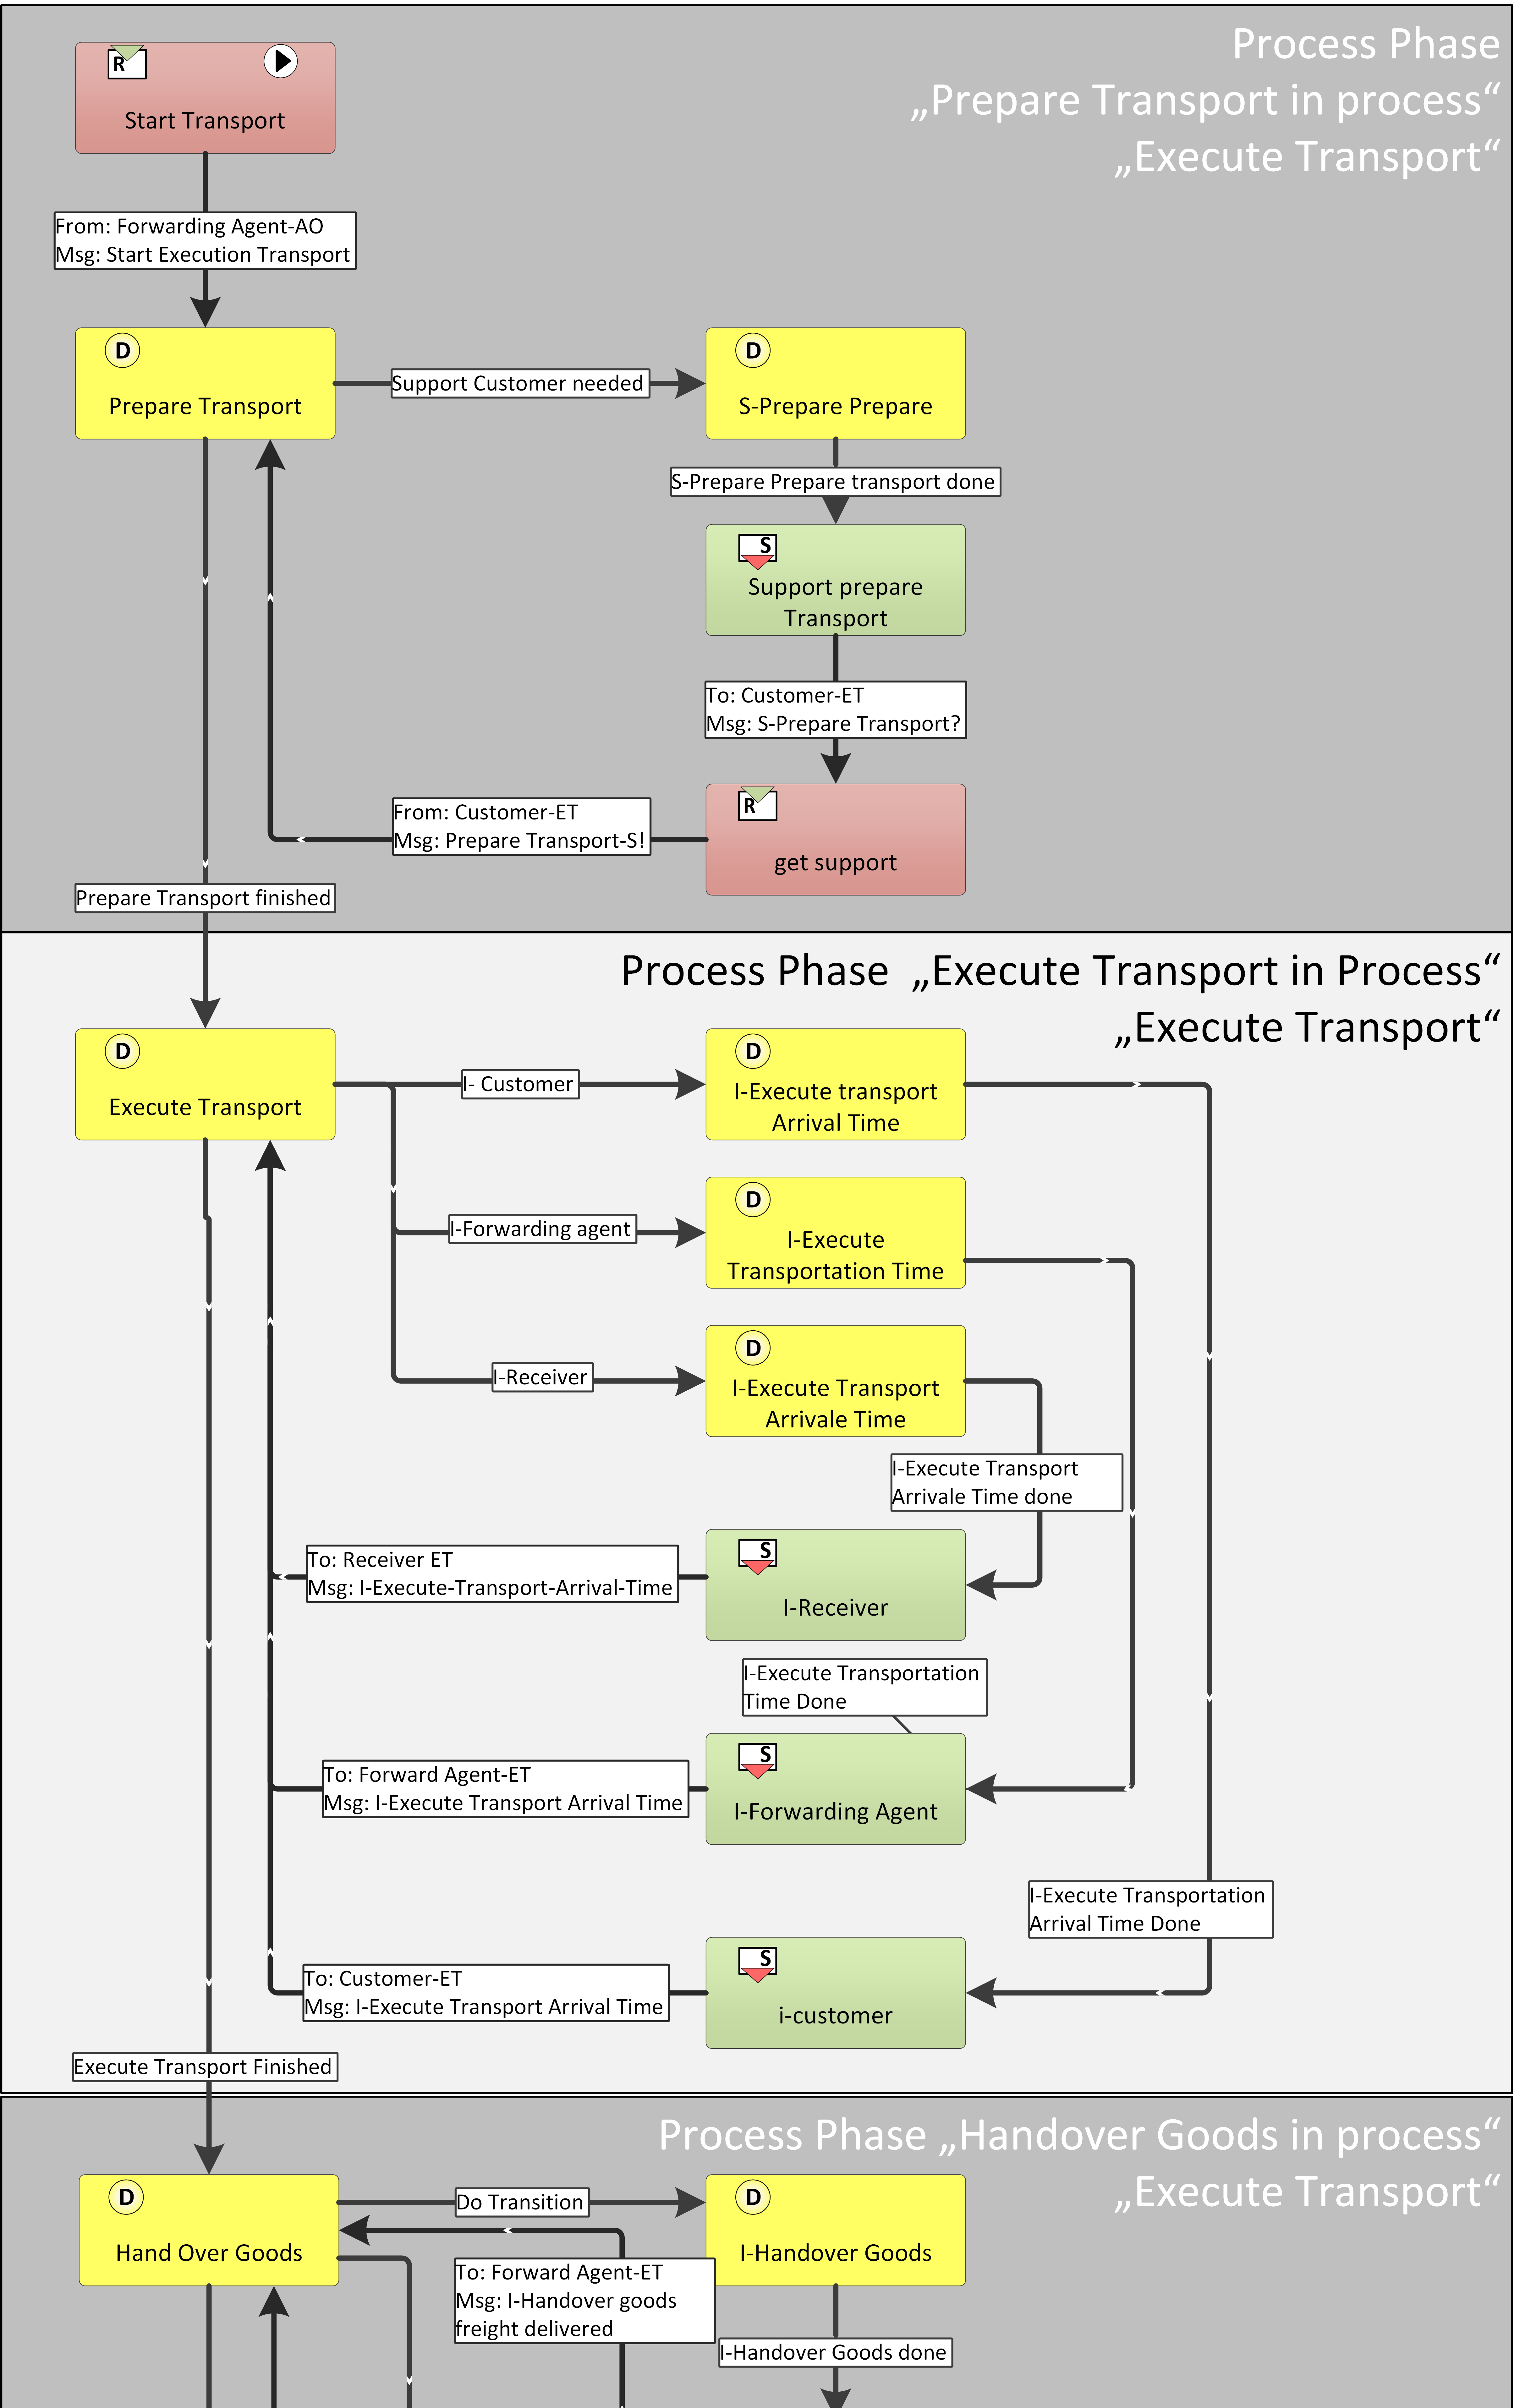
\includegraphics[scale=0.7]{Figures/Chapter5/Subject-Phase/SBD-Carrier-ET_NEW.png}
	\caption{SBD of Subject 'Carrier-ET' in Process 'Execute Transport'}
	\label{fig:SBD-Carrier-ET}
\end{figure}


\subsection{Evaluation of the Transformation}
S-PMs combine SCD and SBD. It show the subjects as active elements in a process, which subjects communicate with each other and which are the major phases of a process. \\

The phases can be seen as subprocesses producing some interim results. The author do not know a general proof that all processes can be structured in phases, but many widely used process specification methods use process phases (see section 'related work'). In his practical work the author hasn't yet found a process which could not structured in 3 to 6 phases, sometimes up to 8 phases (around two out of hundred).
\\
The conversion of each process phase into SCD and SBD is based on modeling by restriction (see chapter 6 in \cite{book:flei2011}). Modeling by restriction is executed in 5 steps:

\begin{itemize}
	\item Identify the number of subjects involved in a process,
	\item give these subjects names which describe their task in the process,
	\item remove not allowed communication paths between subjects,
	\item introduce process specific message names
	\item adapt communication behaviour to process requirements
\end{itemize}

An S-PM contains the information to execute the first 4 steps automatically for each process phase.In a phase the E-Subject communicates with the S- and I-subjects in a not very strict way. This means an E-Subject can request a service from a S-subject as often it wants, which may be not correct in the sense of the considered process. Finally an E-Subject decides whether a succeeding phase is started. This means a S-PM is converted in a process consisting of a chain of not very strictly defined subprocesses derived by modeling by restriction from the S-PM.


\subsection{Activity and Data Details in S-PM}
In S-PM mainly the sequencees of the execution of the major activities are considered.  In order to describe data and the details of the activities executed in a process phase a so called Input Execution Output table (IEO-Table) is used.  The following figure \ref{fig:Inpurt-Execution-Output} shows the IEO-table for the S-PM of the process 'Accept Order'.

\begin{figure}[hbtp]
	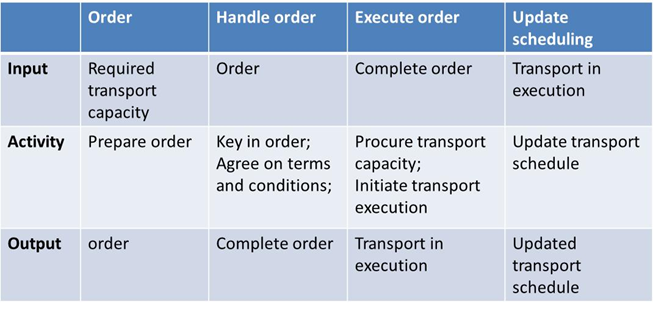
\includegraphics[scale=0.5]{Figures/Chapter5/Subject-Phase/Inpurt-Execution-Output.png}
	\caption{Input Execution Output Matrix of Process 'Accept Order'}
	\label{fig:Inpurt-Execution-Output}
\end{figure}

The columns represent the phases of a process as in the corresponding  S-PM. In the input row the data required in a process phase are specified, in the activity row the activities executed in a phase are listed and the output row contains the results of a process phase. 
The activities listed in the activity row define the details of the internal activity called 'phase name' or 'S-phase name' in a SBD derived from a S-PM. Based on that information the SBD can be described in more detail.
The input and output row can be used to define the business objects used by the various subjects and transported by the different messages.
In order to develop a systematic way to hand over that information to more detailed SCDs and SBD some additional work has to be done and experience has to be gathered. Up to now only a very intuitive approach is used.

\subsection{Conclusion}
S-PMs give managers and subjects involved in process an overview of a process provided that a process can be separated in phases. Practical experiences over more than 10 years show that this is possible without any difficulties. S-PMs are precisely defined which allows to convert them in SCDs and SBDs automatically. This conversion is based on modeling by restriction. This automatic conversion result in a first version of SCDs and SBDs which must be more restricted by the requirements of the considered process and enriched with the required business objects. Details for a S-PM are described in so called IEO-tables which contain details about the required data, the executed activities and the results of a process phase. In further work it has to be investigated how this infomation can be used in automatic conversions.

\subsection{Future Work}
Several aspects and topics need to be addressed by future research:
\begin{list}{-}{spacing}
	\item Definition of structural semantics in OWL
	\item Formal definition of the transformation from a Subject-Phase Matrix to a subject oriented model
\end{list}





\section{Hierarchies in Communication Oriented Business Process Models}

PASS  offers powerful possibilities for structuring complex process systems. The ways to do that are demonstrated with an example.
As an example we will consider a process for realizing a car break down service. This service consists of several connected processes. There is the main process for handling the car accident and supporting e.g. processes for organising towing and repair shop services. Insurance companies may be involved for covering damages, the customer gets an invoice, uses money transfer services or banks for paying the invoice. These processes are executed by various organisations like help desk service companies, towing service companies, car repair workshops banks etc.. In most business process projects not all parts of processes are described in detail. Only a certain part is considered, e.g. only the help desk process has to be considered in detail. In order to do so we have to consider the whole environment in which a considered process is embedded. We have to know which relations exists to these other processes. It is necessary to know which inputs are rquired by neighbour processes and which results they deliver. A help desk process which organizes the towing services has to know how the towing service is requested and which further interactions are required. For instance it must be agreed whether the towing service informs the client about the arrival time of the towing truck or the help desk does it.


\subsection{Process Architecture}

Rectangles represent processes. Each process has a name. Processes consists of other processes and/or subjects. The lines between the rectangles represent the communication channels between processes. Each communication channel has a nameand can contain other communication chan-nels and/or messages.

Figure \ref{fig:car-service-level1} shows the highest process level of the car break down service. In the "car use" process the event "car break down" happens. In order to organize support an interaction is initiated with process "car break down service" . Between these processes messages are exchanged which are elements of the communication channel "Car break down handling".\\


\begin{figure}[htbp]
	\centering
	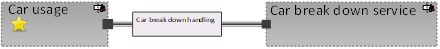
\includegraphics[width=0.7\linewidth]{Figures/Chapter5/figures-hierarchy/Car-Service-Level1.jpg}
	\caption[High level structure of car break down service]{High level structure of car break down service}
	\label{fig:car-service-level1}
\end{figure}



Figure \ref{fig:car-service-leve2} shows the next process structure level of the process "car break down ser-vice". In this level the process "Car break down service" is spltid in 10 processes. The processes "Bank", "Insurance service", "Car repair workshop", "Incident Management","Mobility Manage-ment" and "Towing Management" have a communication channel to the prcess "Car usage". This means the communication channel "Car break down handling" is split into five communica-tion channels. Each of them covers the communication with the relared process, e.g. the communi-cation channel "Accident notification Car break down" is the communication channel between the processes "Car usage" and "Incident Management".\\


\begin{figure*}[htbp]
	\centering
	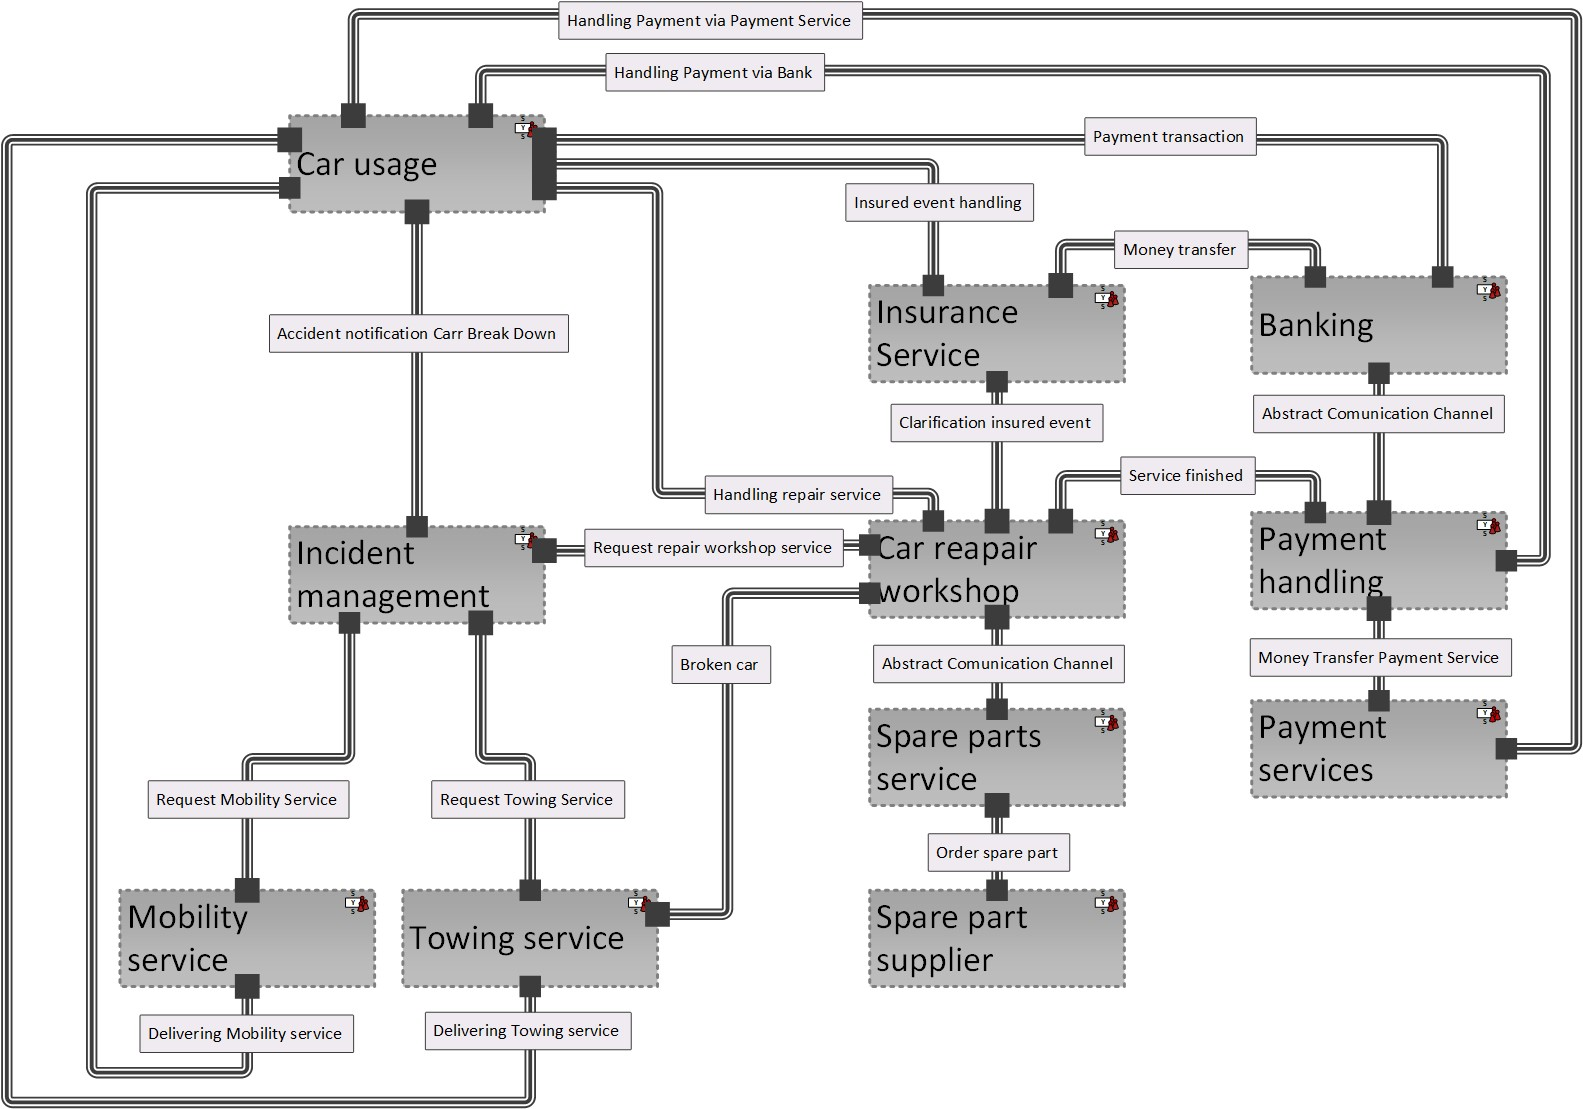
\includegraphics[width=0.8\linewidth]{Figures/Chapter5/figures-hierarchy/Car-Service-Leve2}
	\caption[Structure of the Emmergency Call Handling Process]{Structure of the Emmergency Call Handling Process}
	\label{fig:car-service-leve2}
\end{figure*}



Inside a process there can be also processes. This means that levels of processes can be built. Figure \ref{fig:car-service-lev3} shows the next deeper level of our process hierarchy. The process "Car repair workshop" is structured in six processes. According to this separation the communication sets are also splitted e.g. the communication set "Handling repair service" is splitted into three parts, one part is han-dled by the process "Service scheduling" the other by the process "Car droping" and the third one by the process "Customer Satisfaction".\\

\begin{figure*}[htbp]
	\centering
	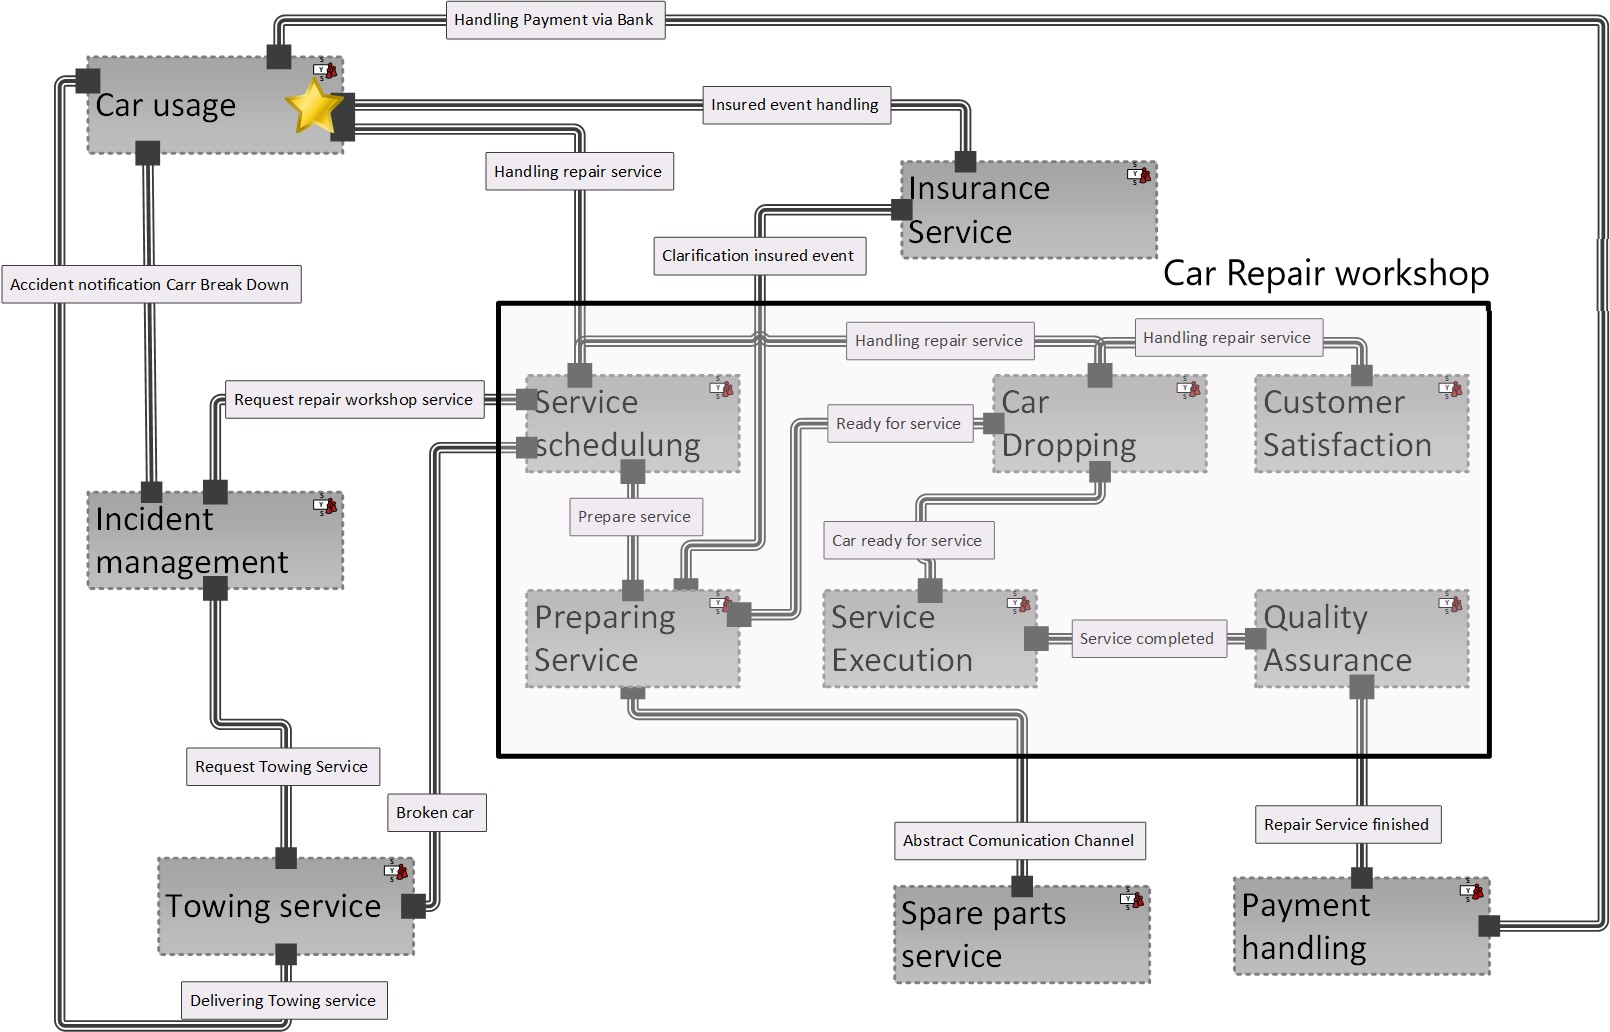
\includegraphics[width=0.8\linewidth]{Figures/Chapter5/figures-hierarchy/Car-Service-Lev3}
	\caption[Details of the "Car repair workshop" Process]{Details of the "Car repair workshop" Process}
	\label{fig:car-service-lev3}
\end{figure*}

As already mentioned, processes cannot communicate directly with each other. The active entities of a process, the subjects communicate with each other. This means messages from one process are sent to an other process are reveived by a subject inside of that process. Messages belonging to a channel are assigned to a sending or receiving subject at the lowest level of a process architecture. This lowest level of a process description is the subject interaction diagram (SID) which shows the involved subjects of a process and the messages they exchange. In the following we consider the process incident management in more detail. This process does not contain other processes like the process "Car Repair Shop". The process "Incident management" contains a Subject Interaction Diagram. Some of the subjects of a process communicate with subjects in other processes. These subjects are called border subjects because they are at the border of a process to other prcesses. Figure \ref{fig:car-service-lev4} shows the process "Incident management" with its border subjects. There is a border subject "Help agent" which communicates with the processes "Towing service", "Mobility ser-vice"and  "Car repair workshop", precisely it communicates with a subject in one of these processes. Another border subject of the process "Incident management" which is called "Help desk"communicates with the process "Car usage".\\

\begin{figure}[htbp]
	\centering
	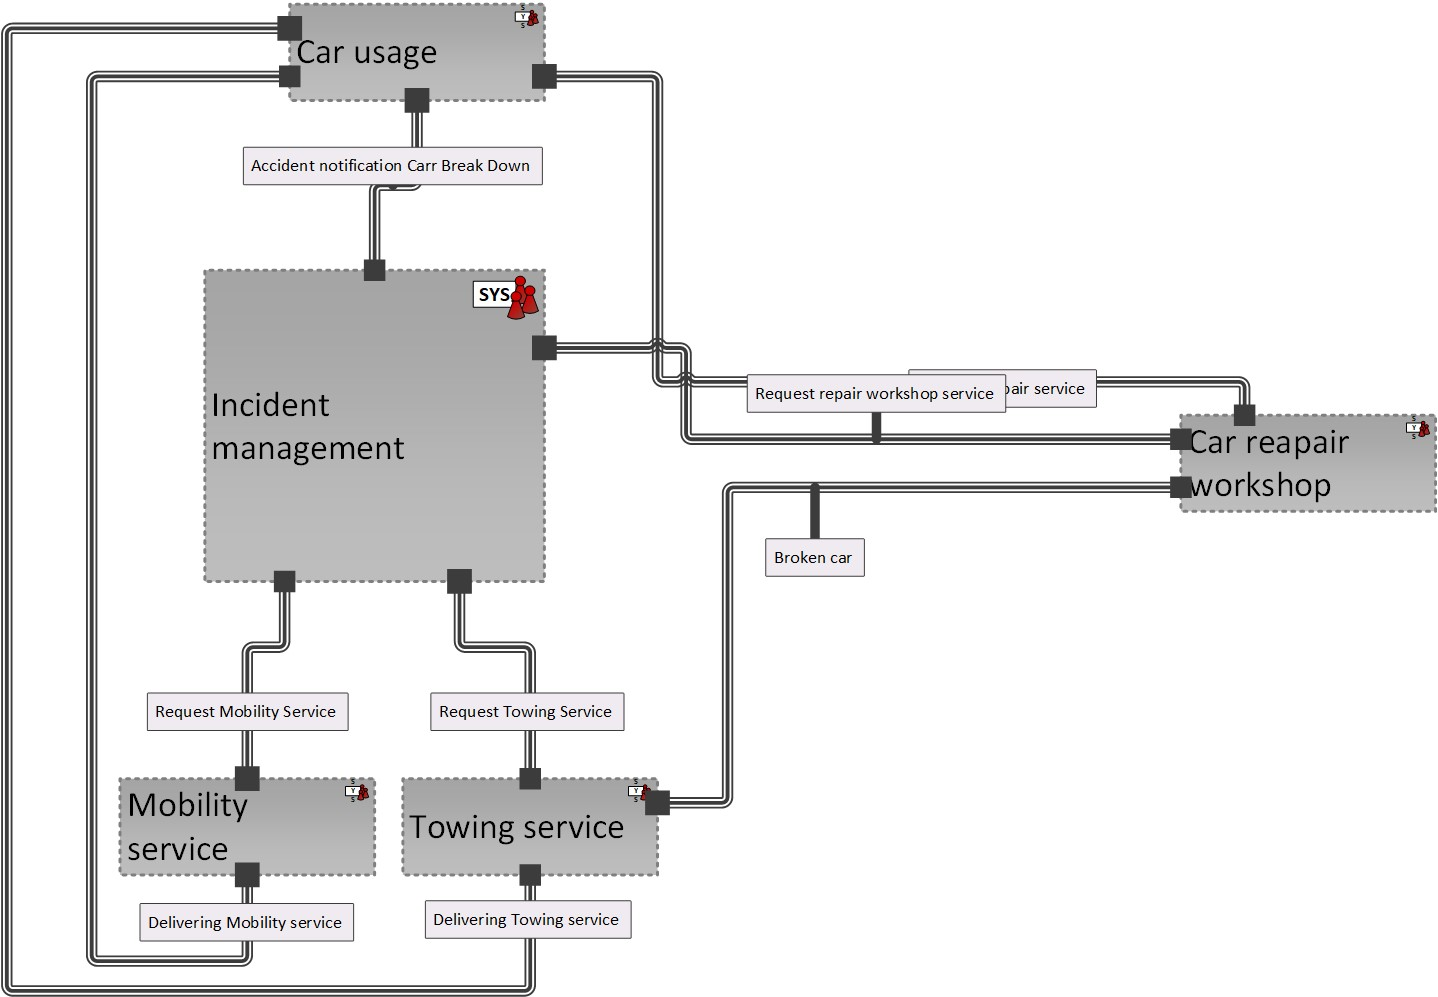
\includegraphics[width=0.9\linewidth]{Figures/Chapter5/figures-hierarchy/Car-Service-Lev4}
	\caption[Neighbors of the "Incident Manaement Process"]{Neighbors of the "Incident Manaement Process"}
	\label{fig:car-service-lev4}
\end{figure}

The border subjects of the process "Incident management" must have a coresponding border sub-ject at the neighbour processes. The border subjects "Call agent" communicates with the border subject "Help requestor" of process "Car usage" and the border subject "Help agent" communi-cates with border subjects of the processes "Car repair workshop", "Towing service and "Mobility service". The process "Incident management" with all the border subjects is shown in  figure \ref{fig:car-service-lev5}.\\

\begin{figure}[htbp]
	\centering
	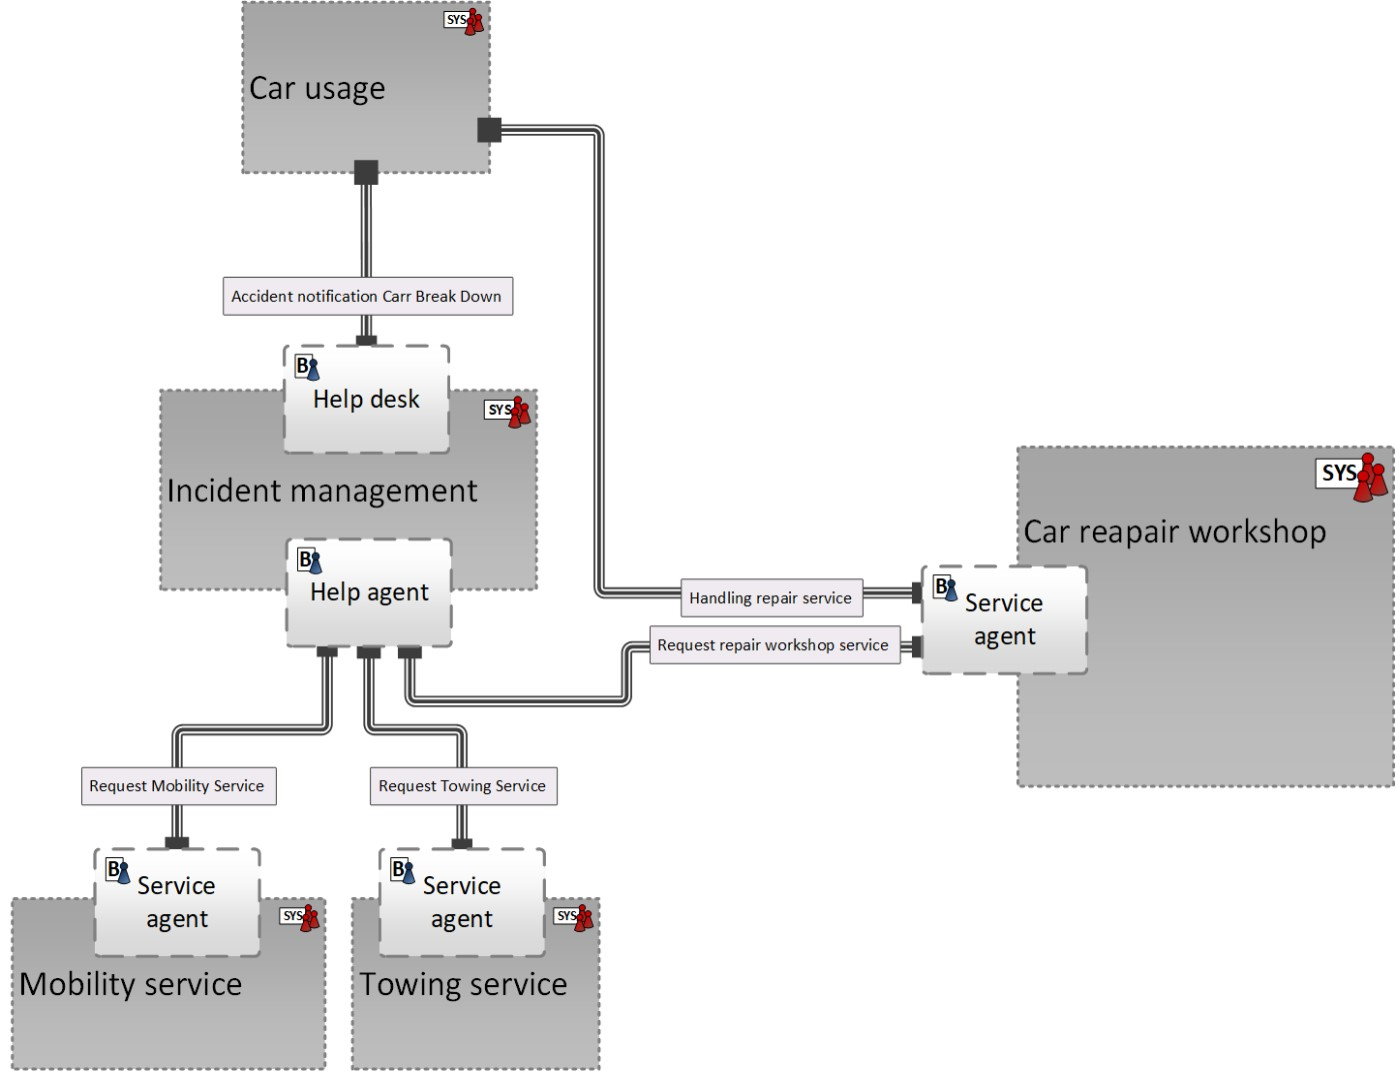
\includegraphics[width=0.9\linewidth]{Figures/Chapter5/figures-hierarchy/Car-Service-Lev5}
	\caption[Border subjects of the "Incident Management" Process]{Border subjects of the "Incident Management" Process}
	\label{fig:car-service-lev5}
\end{figure}

The border subjects of the processes "Mobility service", "Towing service" and "Car repair work-shop" have the same name “Service agent” but these are different subjets because they belong to different processes. Because the process "Car repair workshop" consists of several layers the corre-sponding border subject can be in a process which is part of process "Car repair workshop" in a lower level.\\
From the perspective of the subjects inside of the process "Incident managent" are the border subjects of the processes "Mobility service", "Towing service" and "Car repair workshop" interfaces to these processes, therefore they are called interface subjects in the Subject Interaction Diegram of a process. Figure \ref{fig:car-service-lev6}shows the Subject Interaction Diagram of the process incident management.\\


\subsection{Behavioral Interface}
Processes to which a considered process has communication relationships are called process neighbours or for short neighbours. Now we want to consider the details of the communication relationships between two neighbours. The interface between two processes is defined by the related border subjects and the allowed sequences in which the messages are exchanged between them in a communication channel. As already described above each message is defined by a name and the data which are transported the so-called payload. A border subject observes the behavior of the border subject of the neighbour process and vice versa. Figure \ref{fig:car-service-lev8} shows the border subject "Help desk" of the processes "Incident Management" which communicates with the border subject of process "Car usage".\\

\begin{figure}[htbp]
	\centering
	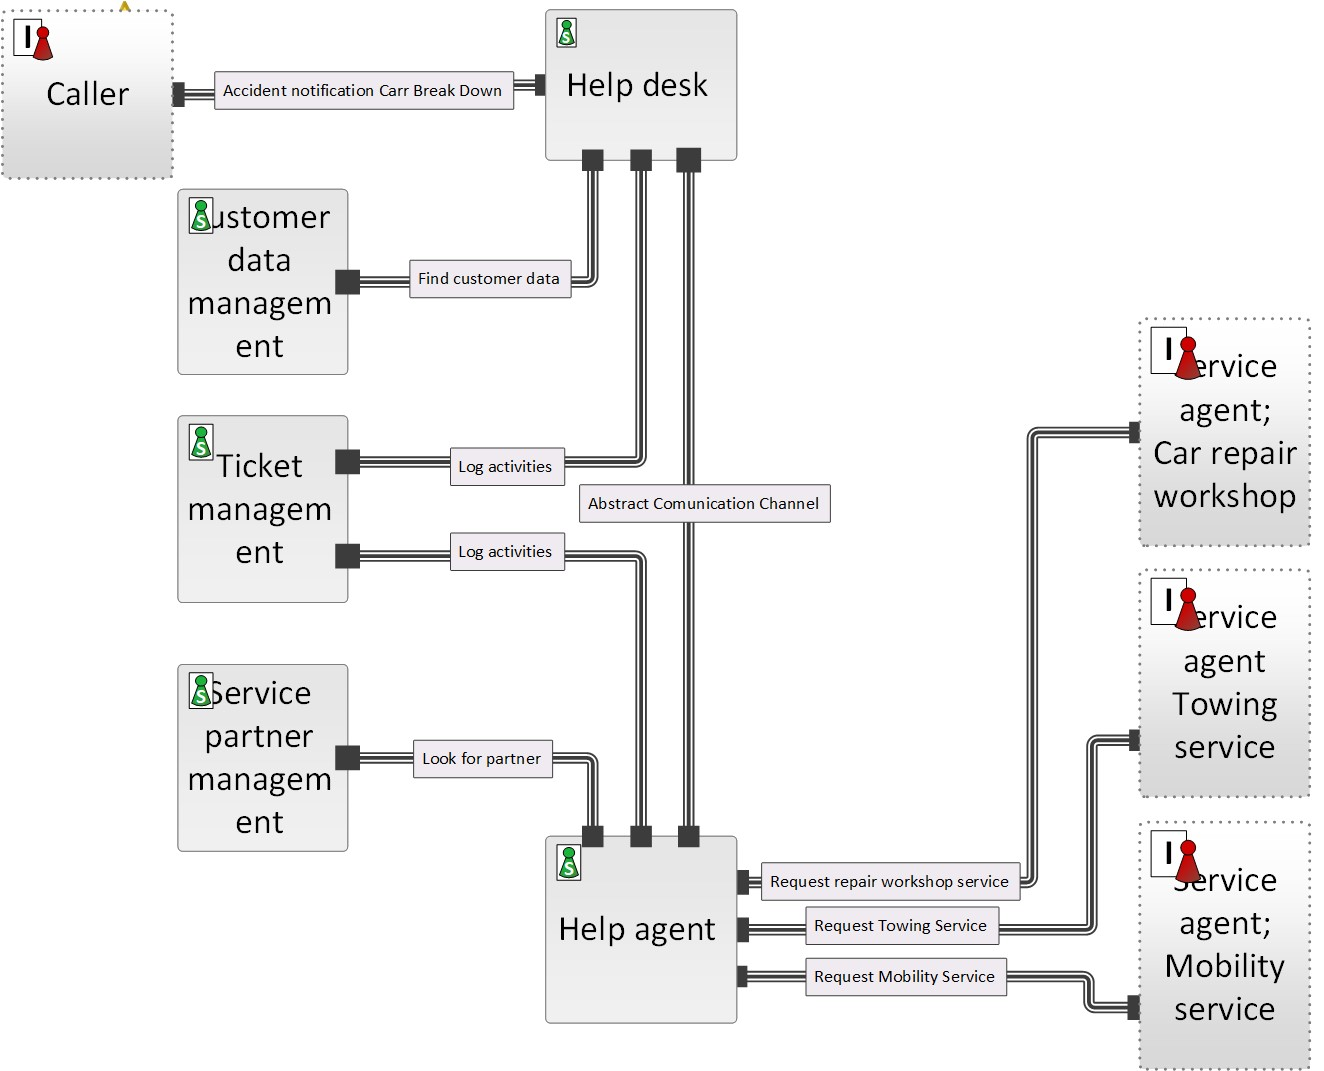
\includegraphics[width=1.0\linewidth]{Figures/Chapter5/figures-hierarchy/Car-Service-Lev6}
	\caption[Subject Interaction Diagram of the Process "Incident Management"]{Subject Interaction Diagram of the Process "Incident Management"}
	\label{fig:car-service-lev6}
\end{figure}

Because we consider the process "Incident management" the border subject "Caller" of the process "Car usage" becomes an interface subject in the SID (details about interface subjects can be found in \cite{Flei12}) of the process “Incident Management”. Figure \ref{fig:car-service-lev8} shows the detailed Subject Interaction Diagram around the subject help desk. \\

\begin{figure}[htbp]
	\centering
	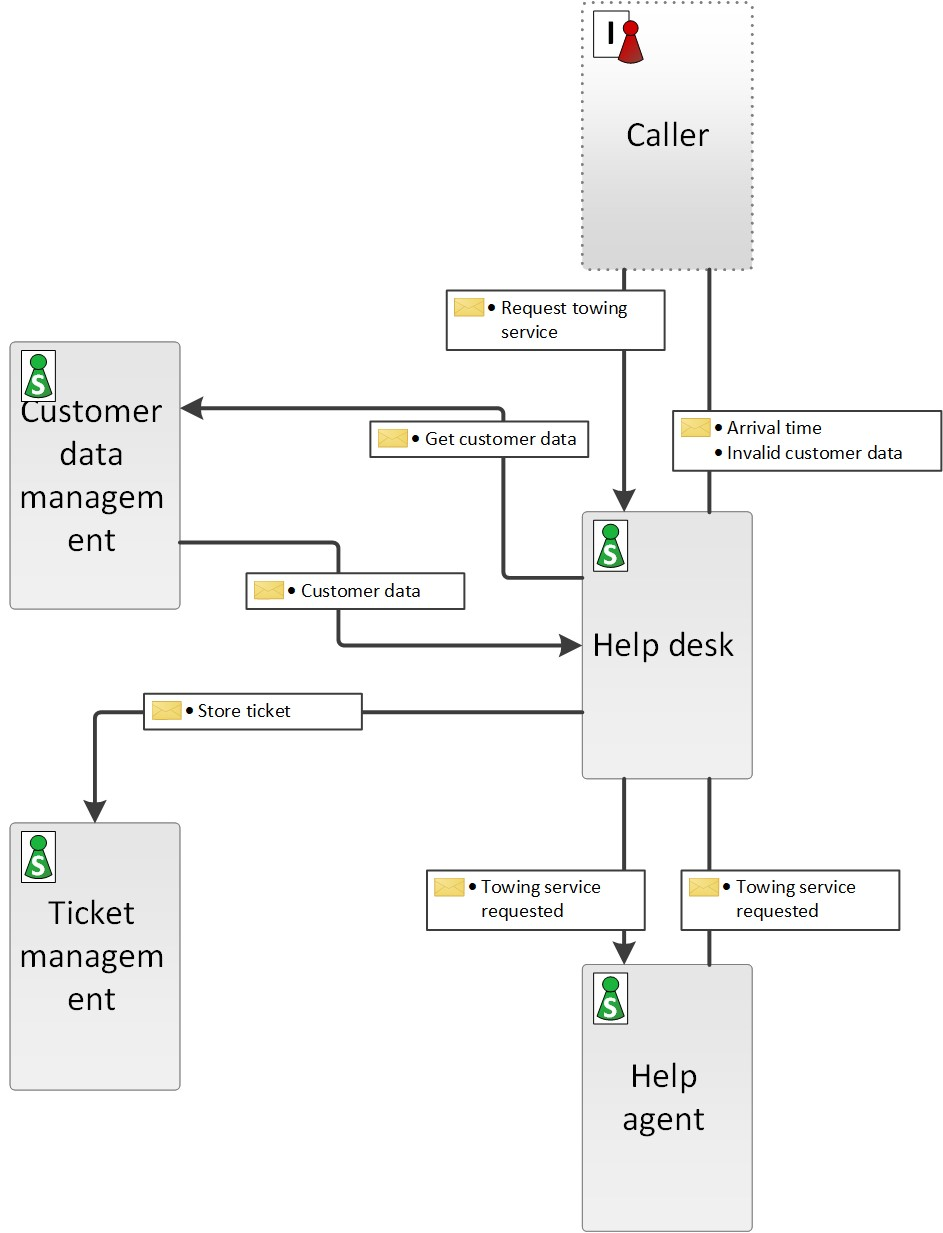
\includegraphics[width=0.9\linewidth]{Figures/Chapter5/figures-hierarchy/Car-Service-Lev8}
	\caption[Subject Interaction around the subject “Help desk”]{Subject Interaction around the subject “Help desk”}
	\label{fig:car-service-lev8}
\end{figure}

Instead of the channels the messages required for a towing service request are shown. A message "Request towing service" comes from the interface subject. This message is accepted by the subject "help desk". The subject help desk checks the customer data received with this message by sending a corresponding the message "Get customer data" to the subject "Customer data management". This subject send the complete customer data back to the subject "Help desk" via the message "Customer data". The subject "Help desk" checks the customer data. If the data are invalid a message "Invalid customer data" is sent to the subject "Caller" and the process is finished.\
If the customer data are valid with that data the subject "Help desk" creates a trouble ticket which is sent to the subject "Ticket management". After that the message "Towing service requested" is sent to the help agent which organizes the towing service. The part of the communication structure of the subject "Help agent" in order to organize the towing service is not shown in figure \ref{fig:car-service-lev9}. We only see that subject "Help agent" sends the message "Towing service data" to the subject "Help desk". This message contains all the data about the service e.g. name of the towing company and arrival time. The subject "Help desk" forwards that data to the interface subject "Caller". This behavior is shown in figure \ref{fig:car-service-lev8}.\\



\begin{figure}[htbp]
	\centering
	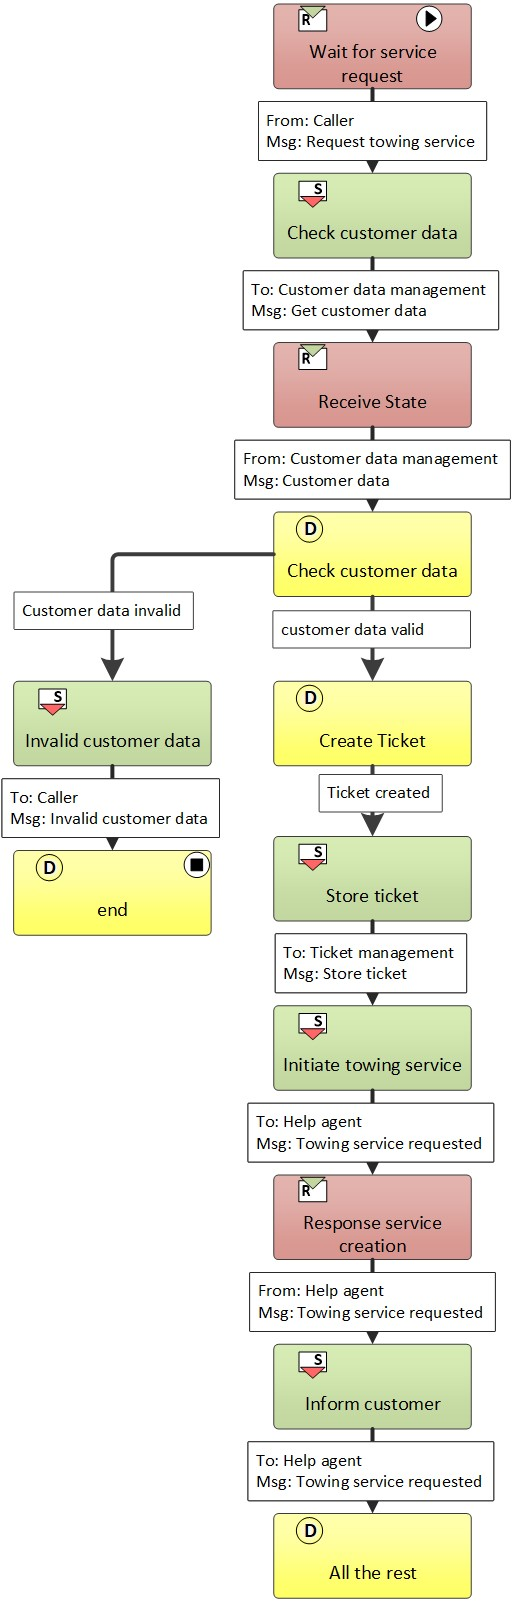
\includegraphics[width=0.7\linewidth]{Figures/Chapter5/figures-hierarchy/Car-Service-Lev9}
	\caption[Part of the Behavior Diagramm of the subject “Help desk”]{Part of the Behavior Diagramm of the subject “Help desk”}
	\label{fig:car-service-lev9}
\end{figure}


The behavior described in the figure above contains the communication with all neighbor subjects of subject "Help desk" including the communication with the interface subject "Caller". From the perspective of this subject the communication of the subject "Help desk" with its other neighbor subjects is not relevant. For the subject "Caller" only the commumication sequence between itself and the subject "Help desk" is relevant. These allowed communication sequences are called the behavioral interface.\\
The behavioral interface between two subjects can be derived from the complete behavior of a subject by deleting the interactions with all the other subjects . Figure \ref{fig:car-service-lev10} shows how the communication sequence relevant for the communication be-tween the subject "Help Desk" and "Caller" is derived from the complete behavior of subject "Help desk".

\begin{figure}[htbp]
	\centering
	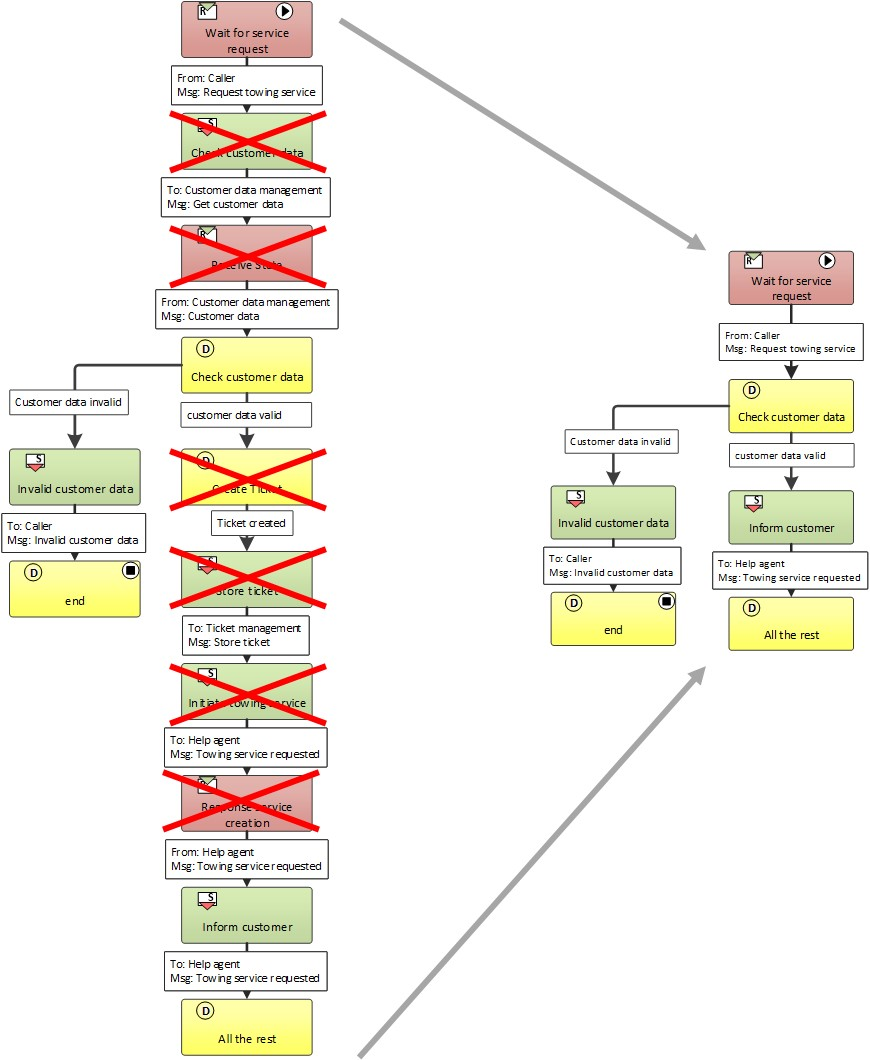
\includegraphics[width=1.0\linewidth]{Figures/Chapter5/figures-hierarchy/Car-Service-Lev10}
	\caption[Deriving the Behavioral Interface from the Subject Behavior]{Deriving the Behavioral Interface from the Subject Behavior}
	\label{fig:car-service-lev10}
\end{figure}

A behavoral interface is always relative to a communication partner. In figure \ref{fig:car-service-lev10} the behavioral interface is relative to the interface subject "Caller". The behavioral interface to the subject "Ticket Management" is different because only the communication activities with this subject are considered.This behavioral interface would be very simple. It consists of only one send activity, sending the message "Store ticket".\\
The behavioral interface relative to a partner subject can be automatically derived from the complete behavior of a subject
(see \cite{article:jCPEX}).

\subsection{Future Work}

Due to the novel conceptual integration addressed, several aspects and topics need to be addressed by future research:
\begin{list}{-}{spacing}
	\item Clarify terminology e.g. using the term interface subject, system interface, implementation
	\item Definition of structural semantics in OWL
	\item Definition of execution semantics in ASM. The semantic of the behaiour interface and its relation to the behavior of the related subject has to be described.
\end{list}


\section{Business Activity Monitoring for S-BPM}\label{sec:BAMinSubjectOrientation}

Monitoring of Business Process looks at running instances. For those it measures metrics, aggregates them to Process Performance Indicators (PPIs) as a business process-related form of Key Performance Indicators (KPIs), reveals deviations (as-is vs. to-be) and report and presents results to people in charge or interested in the value of the PPI. Thus monitoring lays ground for the performance analysis in the key dimensions quality, time and costs of processes and helps identifying weaknesses and opportunities for improvement \cite{book:UntPerform}.
By feeding back information for completed and running instances to analysis monitoring fosters organizational learning, forms an important part of the Business Process Management (BPM) lifecycle \cite{article:SUbjetorientiertBPM} and thus helps implementing the operational level in the closed-loop approach to enterprise performance management \cite{book:processmonitoring} (see figure \ref{fig:Approach-Performance}).
\\


\begin{figure}[htbp]
	\centering
	\includegraphics[width=0.8\linewidth]{Figures/Chapter5/Monitoring/Approach-Performance-Mgmt.jpg}
	\caption[Closed-loop Approach to Performance Management]{Closed-loop Approach to Performance Management \cite{book:AnalytInfSys}}
	\label{fig:Approach-Performance}
\end{figure}



\subsection{Architecture }
A Business Activity Monitoring (BAM) environment supported by Complex Event Processing consists of several elements necessary at build time and at runtime (see figure \ref{fig:BAMArchitecture}) and \cite{book:processmonitoring}, \cite{book:CEPinAction} , \cite{article:BlueprintEventBPM}). At build time a modeling environment should provide tools for designing processes (e.g. Metasonic Build) and defining process performance indicators (PPIs), BAM events, rules, thresholds etc. as well as parameters for their visualization in report and on dashboards. At runtime there are (1) event producers like a process engine (e.g. Metasonic Flow) or an ERP system (e.g. SAP) which feed events into an event cloud or stream (chronologically ordered). (2) Event Processing Agents (EPA) form the event processing logic. They process events based on metrics, event patterns, rules and other parameters specified at design time. Their basic logical functions include filtering and transforming events and detecting patterns among them. Global state elements allow them accessing data from outside the application (e.g. from an ERP system). EPAs put the results of their processing (also to be understood as events) out to Event Consumers (3) like dashboards or process engines. Input and Output Adapters (IA, OA) transform event data between different formats of system elements as necessary. All system elements involved form an Event Processing Network (EPN), in which events are exchanged by communication mechanisms.

\begin{figure}[htbp]
	\centering
	\includegraphics[width=0.9\linewidth]{Figures/Chapter5/Monitoring/Integrated-BAM-CEP-Architecture-27.jpg}
	\caption[Integrated BAM/CEP Architecture 27]{Integrated BAM/CEP Architecture \cite{book:processmonitoring}}
	\label{fig:BAMArchitecture}
\end{figure}



\subsection{Modeling BAM Parameters at Build Time}
As mentioned in the last section it is necessary not only to model the processes, but also numerous pieces of information relevant for a sound process monitoring in the sense of Business Activity Monitoring (BAM model). These can be derived from answers to questions like what, when, how and how often should be measured by whom \cite{book:ProzesseSchmelzer}. The information should also include how single metrics are to be aggregated in order to determine Process Performance Indicators (PPIs). For systematically collecting and documenting the necessary information fact sheets or templates for metrics and performance indicators have been developed \cite{book:KennzahlenIT}, \cite{book:ITControlling}. Figure \ref{tbl:Fact-Sheet}  shows an extract of a sample fact sheet defined for the average processing time of activities (see also \cite{article:SBPMCosting}, \cite{book:MonitoringSubjekt} ).


\begin{table}[htbp]
	\footnotesize
	\centering
	\begin{tabular}[t]{@{}l p{0.5\linewidth} p{0.3\linewidth} @{}}
		\toprule
		\textbf{Attribute} & \textbf{Content} \\
		\midrule
		\\
		 & \textbf{Characteristics}
		\\
		Identifier & Average activity time
		\\
		Description & Average time of a process activity within a certain period
		\\
		To-be value/unit & tbd specifically (min.)
		\\
		Tolerance range/unit & tbd specifically (\%)
		\\
		Escalation Rules/ Actions & In case of violation alert the process owner and start escalation process (tbd specifically)
		\\
		Addressees & Process Owner, Middle Mangement, Accountants (tbd specifically)
		Responsibility	Process Owner (tbd specifically)
		\\
		&  &
		\\
		& \textbf{Measuring and Computing}
		\\
		Measuring Object & All instances of the process 'Purchase Order'
		\\
		(Single) Metrics & Start time and end time of all activities of the process
		\\
		Measuring Method & Read time stamps for beginning and end of activities written by Metasonic Flow
		\\
		Measuring Frequency & For every single instance as it occurs
		\\
		Algorithms & For computing period: Sum of processing time of all activities divided by number of instances

		\\
		Data Sources (general) & Tables in the database of Metasonic Suite:
		RT\_PROCDESC, RT\_PROCINST, REC\_PARADESC, REC\_RECTRANS, UM\_USER
		\\
		Data Sources (specific) & Activity processing time (for one instance):\newline
		\textbf{SELECT} TIMESTAMP1  \newline
		(\textbf{SELECT} STARTTIME \newline
		\textbf{FROM} RT\_PROCINST \newline
		\textbf{WHERE} RT\_PROCDESC = \textit{process (purchase order)}\newline
		\textbf{AND} ID = \textit{instance (9)}\newline
		\textbf{FROM} REC\_RECTRANS\newline
		\textbf{WHERE} RT\_STDESC = \textit{\textit{state (fill\_in\_form)}}\newline
		\textbf{AND} RT\_PROCINST = \textit{instance (9)}
		Completed instances: see separate fact sheet .
		\\
		Computing Period (time, no. of inst.) & Daily
		\\
		& \textbf{Presentation}
		\\
		Presentation Style & As-is value and to-be value in combination with a spark line showing the historical development, deviation from to-be value in \%
		\\
		Presentation Frequency & Weekly and in case of escalation
		\\
		Archiving & Stored in additional database table, linked with RT\_PROCDESC
		\\

\bottomrule
\end{tabular}
\caption{Fact Sheet for a PPI (extract)}
\label{tbl:Fact-Sheet}
\end{table}

Replacing the content column by more formal ontology-based linguistic patterns as suggested by Del-Rio-Ortega et al. (see table \ref{tbl:Fact-Sheet-PPI}) could help relating PPIs to elements of the process model, performing automated analysis \cite{article:ProcessPerfInd} and implementing the measurement at runtime.

\begin{table}[htbp]
	\footnotesize
	\centering
%	\begin{tabular}[t]{@{}1 p{0.3\linewidth} p{0.3\linewidth} p{0.4\linewidth} @{}}
	\begin{tabular}[t]{ p{2 cm} p{5 cm} p{5 cm} }	
	\toprule
		\textbf{Attribute} & \textbf{Linguistic Pattern}  & \textbf{Example}
		\\
		\midrule
		PPI-<ID> & <PPI descriptive name> & PPI-001 Average time of RFC analysis
		\\
		\midrule
		Process	& <process ID the PPI is related to> & Request for change (RFC)
		\\
		\midrule
		Goals & <strategic or operational goals the PPI is related to> & BG-002: Improve customer satisfaction \newline
		BG-014: Reduce RFC time to response
		\\
		\midrule
		Definition & The PPI is defined as \newline \{<DurationMeasure> \newline \textbar <CountMeasure> \newline \textbar <ConditionMeasure> \newline \textbar <DataMeasure> \newline \textbar <DerivedMeasure> \newline \textbar <AggregatedMeasure> \} \newline {[}expressed in <unit of measure>{]} &  The PPI is defined as the average of Duration of Analyse RFC activity
		\\
		\midrule
		Target & The PPI value must \newline \{be \{greater \textbar lower\} than \newline {[}or equal to{]} <bound> \newline \textbar be between <lower bound> and \newline <upper bound> {[}inclusive{]} \textbar \newline fulfil the following constraint: <target constraint>\} \} & The PPI value must be slower than or equal to 1 working day
		\\
		\midrule
		Scope & The process instances considered for this PPI are \newline \{the last <n> ones \textbar those in the analysis period <AP-x> \} & The process instances considered for this PPI are the last 100 ones
		\\
		\midrule
		Source & <source from which the PPI measure can be obtained> &	Event logs of BPMS
		\\
		\midrule
		Responsible & \{ <role> \textbar <department> \textbar <organization> \textbar <person> \} &	Planning and quality manager
		\\
		\midrule
		Informed & \{ <role> \textbar <department> \textbar <organization> \textbar <person> \} & CIO
		\\
		\midrule
		Comments & <additional comments about the PPI> & Most RFCs are created after 12:00
		\\
\bottomrule
\end{tabular}
\caption{PPI Template based on Linguistic Patterns \cite{article:ProcessPerfInd}}
\label{tbl:Fact-Sheet-PPI}
\end{table}





Friedenstab et al. argue that such linguistic patterns do not fit to the usually graphical modeling of processes which makes integration difficult \cite{article:BPMNActivityMon}. The authors discuss some more approaches to BAM modeling. With regard to the limitations revealed, they present a BAM-related extension of the graphical Business Process Model Notation (BPMN) \cite{article:BPMNActivityMon}.
Using an abstract language syntax based on the Unified Modeling Language (UML) they started defining meta models for language constructs needed for BAM as there are Duration, Frequency, Composed Basic Measure, Aggregated Measure, Filter, Target Definition, Actions, Measure-based Expressions and Dashboard. Figure \ref{fig:Meta-Model} depicts the example for the duration of elements on different levels of detail, where the grey colored parts indicate references to the BPMN specification.

\begin{figure}[htbp]
	\centering
	\includegraphics[width=0.9\linewidth]{Figures/Chapter5/Monitoring/Meta-Mode-fo-Duration-relate-to-BPMN-1.jpg}
	\caption[Meta Model for Duration (related to BPMN) 12]{Meta Model for Duration (related to BPMN) \cite{article:BPMNActivityMon}}
	\label{fig:Meta-Model}
\end{figure}


In a second step Friedenstab et al. developed a concrete syntax allowing for modeling the abstract language elements with graphical symbols and text labels. Parts of it are visible in figure \ref{fig:Model-Cycle-Times}. The example shows the BAM model for determining the cycle times of a purchase order process modeled in BPMN (lower part). The upmost part for example expresses the fact that the overall cycle time (Duration) for the last 50 instances (Filter) has to be determined and displayed on the dashboard (Dashboard). Monitoring the average of the overall cycle time for completed instances controls the modeled business logic of the process. If it is above 48 hours goods are delivered with an express shipping if the average cycle time is more than. Otherwise standard shipping is carried out. A deviation also leads to an alert sent to the process owner, while in any case the average is to be presented on the dashboard. The latter is also valid for the third time-related metric in the example, the partial cycle-time for the company-internal part of the process, which is set into relation with the overall cycle time.

\begin{figure}[htbp]
	\centering
	\includegraphics[width=0.9\linewidth]{Figures/Chapter5/Monitoring/BAM Model for Cycle Times.jpg}
	\caption[BAM Model for Cycle Times of a Purchase Order Process based on BPMN 12]{BAM Model for Cycle Times of a Purchase Order Process based on BPMN \cite{article:BPMNActivityMon}}
	\label{fig:Model-Cycle-Times}
\end{figure}


The concept presented by Friedenstab et al. is thoroughly thought-out and clearly and precisely elaborated. The idea now is to adapt it to Subject-oriented Business Process Management and relate the abstract syntax to the S-BPM meta model instead of BPMN. Due to S-BPM being a more precise and comprehensive notation than BPMN \cite{article:BPMNYAWLPatterns} the mapping should be possible without problems. Table \ref{tbl:MonBPMNSBPM} compares the BPMN specification elements used by \cite{article:BPMNActivityMon} with the ones appropriate in S-BPM \cite{Flei12}.


\begin{table}[htbp]
	\footnotesize
	\centering
	\begin{tabular}[t]{@{}l p{0.3\linewidth} p{0.4\linewidth} p{0.5\linewidth} @{}}
	\toprule
	\textbf{BAM Language Syntax Construct} & \textbf{Used BPMN Specification Element}  & \textbf{Suitable S-BPM Specification Element}\\
	\midrule\\
	Duration (Time-Consuming Element) &	Process, Activity, Flow Nodes&	Process, Subject Behaviour States (Function, Send, Receive, Start, End)
	\\
	Frequency
	(Countable Element)&	Process, Activity, Data Objects, Data States &	Process, Subject Behaviour States (Function, Send, Receive), Business Objects and their States
	\\
	Actions &	Process	 & Process
	\\
	Measure-based Expressions &	Expression, Sequence Flow &	Incoming Message
	\\
	\bottomrule
\end{tabular}
\caption{BPMN and S-BPM Specifications used in BAM Constructs}
\label{tbl:MonBPMNSBPM}
\end{table}

The remaining constructs as well as the extensions do not depend on the process modeling language and thus are not included in the table.
On the other hand S-BPM, following its paradigm of regarding subjects, predicates and objects as equally important parts of a process, offers the subject as an additional specification element to add . In figure \ref{fig:Meta-Model-S_BPM} we modified the picture of figure \ref{fig:Meta-Model} by replacing the BPMN by S-BPM elements and adding the subject. This allows modeling the determination of the overall time a subject (respectively the allocated resource(s)) spends on working on a process instance. This is of interest for cost-related analysis.

\begin{figure}[htbp]
	\centering
	\includegraphics[width=0.9\linewidth]{Figures/Chapter5/Monitoring/Meta-Mode-fo-Duration-relate- to-SBPM.jpg}
	\caption[Meta Model for Duration (related to S-BPM)]{Meta Model for Duration (related to S-BPM)}
	\label{fig:Meta-Model-S_BPM}
\end{figure}


In order to show how the BAM language syntax constructs can be related to subject-oriented models we designed the purchase order process in S-BPM. Due to missing information in the BPM model some assumptions were necessary like who performs the process steps (subjects). We then added the BAM modeling symbols to create a monitoring model similar to that in figure \ref{fig:Meta-Model-S_BPM}.
The result is depicted in the following graph. In the lower part it includes the subject interaction diagram (SID) of the process. The SID shows the subjects involved and how they coordinate themselves in the course of action by exchanging messages. In the monitoring model in the upper part a difference can be seen. The partial cycle time for the company-internal activities can be modeled by just relating the clock symbol to the subject "Sales". In the example this subject represents all steps carried out within the organization. In the same way we can determine the cycle time for the other subjects.

\begin{figure}[htbp]
	\centering
	\includegraphics[width=0.9\linewidth]{Figures/Chapter5/Monitoring/BAM-Model-fo- Cycle-Times-of-a-Purchase-Order-Process-based-on-S-BPM.png}
	\caption[BAM Model for Cycle Times of a Purchase Order Process based on S-BPM]{BAM Model for Cycle Times of a Purchase Order Process based on S-BPM}
	\label{fig:Cycle-Time-SBPM}
\end{figure}

Given a special information demand a more granular modeling of BAM parameters is possible on the subject behavior level. Figure \ref{fig:BAM-Cycle-Time} for example details the behavior of "Sales" including all receive, send and functional states walked through by the subject. The symbols indicate that the average cycle time between order reception and confirming the order to the customer should be measured. In the same way cycle times between states in behaviours of different subjects can be modelled.


\begin{figure}[htbp]
	\centering
	\includegraphics[width=0.9\linewidth]{Figures/Chapter5/Monitoring/BAM-Model-for-Cycle-Time-of-a-Process-Section-based-on-S-BPM.jpg}
	\caption[BAM Model for Cycle Time of a Process Section based on S-BPM]{BAM Model for Cycle Time of a Process Section based on S-BPM}
	\label{fig:BAM-Cycle-Time}
\end{figure}

Back on the level of subject interaction diagram we could also model to determine the overall time for receiving (waiting), sending and doing, both by process and by subject. Modeling on the two diagram levels reduces complexity.

\subsection {Conclusion and future Work}
This contribution systematized Business Process Monitoring and shed some light on the current state of monitoring in the context of S-BPM. Starting there we emphasized Business Activity Monitoring and took a closer look to the modelling of BAM parameters. We showed that the approach for BPMN presented by Friedenstab et al. can be adapted to S-BPM with little effort and that S-BPM shows additional potential to further develop the concept.
\\
\subsection{Future Work}

Due to the novel conceptual integration addressed, several aspects and topics need to be addressed by future research:
\begin{list}{-}{spacing}
	\item Extension of the structural semantics in OWL with possibilities to add Process Performance Indicators
	\item ASM definition of execution semantics for throwing events if process performance indicator bounderies are violated.
	\item ASM definition of execution semantics for handling violation events
\end{list}


\section{Subject Oriented Project Management}

Subject orientation is focused on networks of indeppendent systems, which coordinate their cooperation by exchanging messages. The involved system may belong to different organisations.
In our global economy enterprises cooperate around the globe in order to create services or manufacture products for customers which are also distributed all over the world. The challenge of the cooperating partners as a federation of independent systems (virtual enterprise, VE) is to establish smooth cross-enterprise communication to reach the common objectives \cite{article:VirtualEnterprise}. Information and communication technologies (ICT) are essential to create a federation of independent software systems suitable to execute business processes across the involved companies.
\\
Figure \ref{fig:DogFoodShop} shows an example of an order-to-cash scenario where federated applications support a cross-company business process. A dog food store sells its products via internet. It commissions a transportation service provider to deliver the ordered products to the customer, who confirms the reception of the goods. The store deducts the money from the customer's bank account. The process steps are facilitated by several independent software applications and message exchanges (order, order confirmation, delivery notification etc.) enabled by respective communication systems.


\begin{figure}[htbp]
	\centering
	\includegraphics[width=0.6\linewidth] {Figures/Chapter5/Project/DogFoodShop.jpg}
	\caption[Order-to-cash scenario in a federation of enterprises and applications (simplified)]{Order-to-cash scenario in a federation of enterprises and applications (simplified)}
	\label{fig:DogFoodShop}
\end{figure}

Developing such a mutually adjusted solution by a federation of independent enterprises requires a project management approach different from traditional software development projects taking a process perspective (cf. \cite{book:ProjectHistory}). Therefore our focus is on how to implement loosely coupled systems for exchanging information between independent partners, rather than tightly coupled solutions for sharing information or other resources.
The section is structured as follows. First software development methodology and its elements are reviewed with respect to developing federated systems. This leads to our proposal of a software development approach for federated systems based on subject orientation.
\\
\subsection{Background}

\subsubsection{\textbf{Recommendations for creating federated systems}}
When independent enterprises develop a federated system a lot of managerial and technological aspects have to be considered, particularly with respect to managing collaborative business processes. This is reflected in the following recommendations (cf. \cite{book:PMThirdWave} , \cite{ChallengesDistPM} ):
\begin{enumerate}
	\item Start the foundation of a federation and identify members.
	\item Identify and describe the business services that organizations can provide or they need from partners in service level agreements.
	\item Harmonize the enactment of collaboration by coordinating the participating organizations according to defined business processes and identify the systems required for the federation.
	\item Integrate the identified and implemented services/systems into the intended application.
	\item Maximize the autonomy of organizations when collaborating, thereby ensuring organizations to benefit most from their own business objectives.
	\item Represent the partnerships between collaborating organizations when collaborating, and update changes in partnership.
	\item Guarantee the business privacy of organizations in the course of collaboration.
	\item Allow partners and other third parties to monitor, measure, and oversee the execution of business processes.
\end{enumerate}


\subsubsection{\textbf{Federation of enterprise information systems}}
\cite{article:VirtualEnterprise} define virtual enterprises and federations of enterprise information systems as follows: "\textit{The Enterprise partners' Virtual Enterprise (EP VE) is the federation of partners in the community that come together to achieve the goal of a federated distributed system environment, sharing their resources, and collaborating to achieve a common goal: the Federated System VE (FS VE). The partners in the federation retain autonomy over their resources, deciding which resources (personnel, resource dollars, equipment, etc.) are sharable for achieving this goal. The results of this VE are then useable by the partners in furthering their individual systems. The FS VE is seen to be a virtual system of distributed processing components (hardware and software), which are physically implemented and managed by the partners. It is a federation of the partners' systems, where each system retains its autonomy over all processing system components and sharable data/information. Retaining autonomy means defining which data or information and software/hardware assets will participate in the federation and be accessible and usable by other systems in the federation.}"\\
The definition shows that the focus is on sharable resources. This means when setting up a federation the VE members need to clarify ownership of the shared resources as well as access rights and the rights to change those. Such an approach often implies tight coupling of the involved enterprises and the related resources. Entities leaving a federation then cause difficulties with respect to separating involved systems (changing access rights) and sorting out ownership of information.
Alternatively, information can be exchanged between the partners by messages, implying only a loose coupling of the involved systems. In this case the partners only need to agree upon structure and meaning of the data, e.g., using XML schemes, and upon the implementation of the message exchange, e.g., by web services.
\\
\subsubsection{\textbf{Software development methodology}}
\textit{"A software development methodology is a collection of procedures, techniques, tools and documentation aids which help developers to implement software systems"}  \cite{book:ISDevelopment}. It may include modeling concepts, tools for model-driven architecture, integrated development environments (IDEs) etc. The so-called magic triangle (see figure \ref{fig:Triangle}) summarizes the various aspects of a software development methodology \cite{book:SoftEng}.

\begin{figure}[htbp]
	\centering
	\includegraphics[width=0.6\linewidth] {Figures/Chapter5/Project/Triangle.jpg}
	\caption[Magic triangle of software development methodologies]{Magic triangle of software development methodologies}
	\label{fig:Triangle}
\end{figure}

Concepts and Techniques are used to create models of the software to be implemented, and are thus significantly influencing which languages, procedures and tools are utilized. The applied concept implies the artifacts to be produced, of which the executable software system is the most important one. The Language is used to create the artifacts and tools. Procedures describe the sequence in which the activities for creating the various artifacts are executed. While languages and tools can be replaced without impacting concepts and procedures, the latter are decisively determining the shape of a software development environment.
\\
\subsubsection{\textbf{Modeling concepts}}
Developing a federated system like the dog food store requires modeling cross-company business processes and the entities performing activities in these processes.
\paragraph{Business process modeling}
There are various approaches for specifying business process models. IT implementations of those models are called process-controlled applications [7] or workflows. The modeling approaches can be distinguished in three classes: (i) Control flow-based specifications put the focus on the activities. (ii) Object-based models mainly describe business objects and the sequence of operations to manipulate them. (iii) Communication-based models focus on the active entities in a process which exchange messages in order to coordinate their work.
By their nature the latter are promising candidates for modeling federations of systems. Business Process Model and Notation (BPMN), the currently most widely discussed modeling language, contains elements for the description of control flows and communication in business processes. In the following we discuss its communication-oriented features.
To model communication BPMN provides so-called pools, each representing a process that can exchange messages with processes in other pools. Conversation diagrams are the means to describe this mechanism: However, they do not allow specifying the sequence in which messages are exchanged. Although the sequence can be captured by collaboration diagrams, the semantics of sending and receiving messages is not precisely defined. For instance, it remains unclear whether messages are exchanged synchronously or asynchronously. Additionally a certain message from a pool can only be received in a single activity state, but not in other states. Choreography diagrams in BPMN also define the allowed message sequence between pools. [8] describe a choreography-based tool for specifying global processes. The problem is that choreography specifications cannot contain data. As a consequence a modeler can only describe message sequences being covered by regular expressions, which is the lowest level in the Chomsky hierarchy. This fact makes it impossible to model a behavior like the following: Pool S sends n messages of a type X to pool R. After that S sends a message Y to R. Subsequently S expects m messages of type A from pool R, which received the n messages of type X. The reason for that is that the messages cannot be counted, because data are not allowed in BPMN choreographies.
Given these properties of BPMN this notation has significant draw backs for modeling communication, hindering the precise development of federations of systems.

\paragraph{Multi-agent systems modeling}
The term agent has multiple meanings. We follow the definition given in [9]: An agent is an entity that performs a specific activity in an environment of which it is aware and that can respond to changes. A multi-agent system (MAS) is a system where several, perhaps all, of the connected entities are agents. The most important property of agents is their controlled autonomy: They independently execute their role-specific behavior, and in multi-agent systems they communicate with each other. These properties are alike those of federated systems which therefore can be considered as multi-agent systems. This means that software development methodologies for agent-oriented software (for an overview see [8]) can help developing federations of applications.
\\
\subsubsection{\textbf{Procedures}}
Software Life Cycles (SLC) build a framework for software development procedures. All software development projects follow a series of phases. While software life cycles can be defined in many different ways, each of them comprises the following generic activities:
\begin{list}{-}{spacing}
	\item Project conception or initiation
	\item Planning
	\item Execution with specification and implementation activities
	\item Termination
\end{list}

In the traditional waterfall approach these activities are performed in the sequence shown above. Other life cycle concepts propose overlapping the development steps, suggest alternatives like the V model or agile development procedures like Extreme Programming and Scrum. \cite{article:ObjectOrientedSWdev}, \cite{book:SoftEng} and \cite{book:ISDevelopment} give an overview of the various approaches.
\\
\subsubsection{\textbf{Work break down structure (WBS)}}
The work break-down structure describes the artifacts to be created in a project in a hierarchical way. A work break-down structure element may be a product, data, service, or any activity results contained in the software life cycle or any combination thereof. A WBS also provides the necessary framework for detailed cost estimating and control along with guidance for schedule development and control. The top level of the WBS should identify the major phases and milestones of the project in a summative fashion. Consequently, the phases used in the top level depend on the software development methodology applied in a project. The first level can either represent the phases used in the software life cycle or the major artifacts of the system to be developed. In case the top level is SLC-oriented it might be built by requirement specification, software architecture, programming, test etc. In the case of an evolutionary life cycle there will be topics like Release 1, Release 2 etc., followed by headlines like requirement specification on the second level.
Another alternative is to use top level headlines corresponding to artifacts created by modeling activities, such as 'create communication structure' or 'describe subject behavior'.
\\
The WBS is created during the planning phase of a project life cycle. During this phase the project manager works with the project team to make sure that the client's needs are addressed and the project is planned completely and approved by the client prior to any sort of production beginning on the project.

\subsubsection{Organisational break down structure and software architecture}
An organizational breakdown structure (OBS) complements the WBS and resource breakdown structure of a project. Project organizations can be broken down in much the same way as the work or product. The OBS is created to reflect the strategy for managing the various aspects of the project and shows the hierarchical breakdown of the management structure. Hence, the work break down structure has a significant impact on the organizational structure of the project team. The same holds for the phases of the software life cycle and the system architecture influencing the work break down structure. Conway’s law states “organizations which design systems ... are constrained to produce designs which are copies of the communication structures of these organizations” \cite{article:ConwaysLaw}. A variation of Conway’s law can be found in [12]. "If the parts of an organization (e.g., teams, departments, or subdivisions) do not closely reflect the essential parts of the product, or if the relationship between organizations do not reflect the relationships between product parts, then the project will be in trouble... Therefore: Make sure the organization is compatible with the product architecture” \cite{book:OrgPatternsAgile}.
As we look at developing federations of systems with a federation of independent project teams, the system architecture needs to be aligned with the multiple project team structure.
\\

\subsection{Software Development Methodology For Federated Systems}
The software development methodology for federated systems proposed here is based on Subject-oriented Business Process Management (S-BPM)


\subsubsection{Development as a multiple-team structure}
We now assume that the dog food order-to-cash scenario does not yet exist. The store wants to extend its services for the customers by offering online shopping and home delivery. In order to reach this business objective it takes the initiative to found a federation of enterprises which combine their services and develop a corresponding federation of systems.
Each federated enterprise establishes a project team, working on their parts of the solution independent from each other. This leads to a multiple-team project on the federation level \cite{book:OrgPatternsAgile}. As the teams belong to different, independent companies they all have their own development culture and methodology.
Since there is no single line management who can assign an overall project manager, the federation members need to agree on a project leader and the competencies related to this role. As the initiator of a federation has the most interest in the development of the federated solution it might be helpful that this company, in our case the store, recruits the leader.

His or her major task is to ensure smooth communication between the independent teams, respectively their managers. The project teams needs to coordinate how the systems they are developing communicate with each other. Their major communication paths are predefined by the communication structure of the system federation. This strategy leads to a high socio-technical-congruence. Figure \ref{fig:Multiple-team} (CS: no missing) shows the team and communication structure of the dog food order-to-cash federation.

\begin{figure}[htbp]
	\centering
	\includegraphics[width=0.6\linewidth] {Figures/Chapter5/Project/MultipleTeam.jpg}
	\caption[Multiple-team project and its communication structure]{Multiple-team project and its communication structure}
	\label{fig:Multiple-team}
\end{figure}

Beside that top-level communication implied by the problem structure, each team can use services offered by other enterprises. Figure 6 reveals that the shipment company uses the service of carriers and forwarding agents, in order to implement the transportation service offered to the dog food shop. This communication relation is of no interest for other federation members and thus should not be visible to the top level teams. It belongs to the internal issues of the shipment project team.
\\
\subsubsection{Development process for federated systems}
 The artifacts to be created according to subject orientation need to be developed by a federation of teams related to the subject interaction structure.

\paragraph{Specification of the communication structure}\
The communication between the various members of the federation needs to be specified in more detail. This is done by assigning a subject to each member of the federation and defining the messages exchanged between the subjects. Together with the data transported by the messages a communication model of the system federation is defined. The advantage of the subject-oriented approach is that the system communication structure is directly in line with the communication structure of the corresponding developing teams. The result of that step is the subject interaction diagram (SID).

\paragraph{Specification of the subject behaviour}\
After defining the communication structure the behavior of each subject is specified. The modelers describe the allowed sequence of messages exchanged on top level and the internal functions of the individual systems. These internal functions represent the services executed by the corresponding federation partner either directly or supported by other service providers. They also encapsulate the communication with those sub-contractors as it is of no interest on the top level of the federation.\\
The behavior of a subject is mainly defined by the corresponding project team, however, in close coordination with the teams responsible for the partner subjects. The teams only need to make sure a message sent to a partner has a receive state in the corresponding subject behavior and vice versa. This pairwise coupling means, e.g., that the behavior description of the shipment company has to contain a state for receiving the “Transfer order” message, transmitted by the related send state in the behavior diagram of the dog food store subject. In order to correctly model these interactions the responsible project teams need also to agree on the interaction sequence of the subjects. However, their internal task behavior (i.e. sequence of functions for task accomplishment) might not become visible to others, as is specified decentralized and might not be shared at all.

\paragraph{Implementation of the input pool}\
The input pool is the abstract concept for defining the semantics of message exchange. Partners exchanging messages need to agree on how they implement the input pool semantics. Sending requires the sending subject to execute a function to deposit a message in the input pool of the receiver. For each subject doing so an implementation agreement is necessary. Since an input pool is owned by exactly one subject, the functionality for accessing it is local and does not need to be coordinated with the partners. In most cases input pools are implemented as web services.

\paragraph{Implementation of subject behaviour}\
Each team has to implement the behavior of its subject. This means they have to ensure that depositing and removing messages (including business objects) in or from the input pool are executed and internal functions are invoked in the specified sequence. Workflow engines are appropriate tools for implementing that functionality.\

\paragraph{Implementation of internal functions}\
The internal functions realize the kernel of the service contributed by a partner to a federated application. Messages are the means to cause the invocation of an internal function, and they transport its result to a partner subject. Internal functions can be based on existing systems, e.g., an SAP client.  They also can be implemented using another federated solution, or being developed from scratch. The way an internal function is realized is a local decision taken by the corresponding project team.

\paragraph{Operation of a federated system}\
Beside the development and deployment the non-functional aspects of a federated system need to be agreed upon by the contributing partners. For this purpose they negotiate service level agreements (SLA) defining response time, down time, reaction time in error cases etc. The SLA also includes business aspects like costs and regulations for exceptional situations like a member leaving the federation and bringing in another one.

\subsubsection{\textbf{Federated work break down structure}}
The various activities described so far can be organized in a federated work break-down structure as shown in figure \ref{fig:WBSDog}.

\begin{figure}[htbp]
	\centering
	\includegraphics[width=0.6\linewidth] {Figures/Chapter5/Project/WBSDog.jpg}
	\caption[Work break down structure for the development of a federated system]{Work break down structure for the development of a federated system}
	\label{fig:WBSDog}
\end{figure}

The tasks can be divided into three types:
\textbf{Joint work} concerns the top level of the federation and therefore is done collaboratively by all members of a federation. The major issue on this level is to agree on communication structure and behavior of the entire system, while the behavior of each subject can be described individually by the corresponding member of the federation.\\
\textbf{Some work can be done bilateral}. Communicating partners, e.g., agree on the coding of the business objects and the implementation of the input pool. They also define the service level agreements.\\
\textbf{Local work} comprises activities of the development teams which do need to be coordinated with teams of other federation members. A major example in this context is the set of internal functions of each subject, being a local matter, and developed following the particular culture and methodology of the respective team.
\\


\subsection{Conclusion}
We have presented an approach for developing federated systems. The concept considers the characteristics of virtual enterprises combining the services of the partners to satisfy customer needs while keeping legal, organizational, technological and cultural independence.
Our communication-oriented view follows the idea that the decentralized structure of federated systems needs to be reflected in the organizational structure of multiple project teams for developing such systems. Those teams belong to separate enterprises and are mutually independent with respect to methodology, technology etc. they use to develop their individual part of the federated system.
The proposed approach establishes a layer above the enterprise-specific environments. It helps building coherence on the top level of the federated system solution, while the teams, system elements etc. on the individual level of each federation member keep the highest degree of independence.

\subsection{Future Work}
It has to be investigated whether the OWL definition and/or the execution semantics has to be adapted for a better project management support. Based on that results some guidelines for a subject oriented project management has to be developed and enhanced based on practical experiences.


\section{Subject-Oriented Fog Computing}

Many scenarios related to digitalization increasingly (i) require an easy-to-customize development environment, (ii) capture on-the-edge systems or devices under the control of users or responsible stakeholders. Typical examples are home support systems in healthcare, maker environments producing local goods, and intelligent transport control systems for smart regions. Developing such applications requires architectures that allow to network or compose systems in a modular, while effective and efficient way \cite{article:SurveyCompConcepts}. During the last years, with the advent of advanced equipment and technologies, such as production devices for the private consumer market, networked applications have become common. As a consequence of this trend, a significant issue also appears, namely the increases in the demand of both communication and execution capability. New applications, such as home care support systems, all deal with complex interaction operations, which should be understood by users, and thus require a high level of abstraction \cite{article:FogHealthcare},\cite{article:MobilecloudComp}.
\\
Such demands pose significant challenges to existing development paradigms, particularly in terms of edge computing and stakeholder-oriented communication capacities (cf. \cite{article:SurveyCompConcepts},\cite{article:FogHealthcare}]). Using behavior abstractions aligning stakeholder needs with communication and processing capabilities in this context is an appealing idea. For instance, in-situ care support devices can be utilized to handle the tasks of preparing the pharmacy order or they can be employed to collaborate with each other to transmitting maintenance messages and sharing resources \cite{article:FogHealthcare}. Besides network technologies, mobile cloud computing is a typical enabler for this demand \cite{article:MobilecloudComp}.\\
However, according to Syed et al. \cite{article:FogPattern} purely cloud-based systems typically require low latency, support for heterogeneity, mobility, geographical distribution, location awareness, etc. Consequently, Fog Computing (FC) as a near-the-edge-computing paradigm has been defined as a collection of various small distributed clouds deployed closer to the systems or devices at the edge of a communication network (ibid.). Fog applications can be structured along several dimensions, either directly or indirectly referring to stakeholder interaction \cite{article:OoTAnalytics}:
\begin{list}{-}{spacing}
	\item Geo-distribution: wide (across region) and dense - high population of events, such as ramp accesses in traffic, sensor systems in production halls, clustering medical devices in home healthcare application development
	\item Low/predictable latency: tight within the scope of a certain location - intersection, production isle, treatment room
	\item Fog-cloud interplay: data at different time scales - sensors at intersection/traffic info at diverse collection points, supply chain monitoring/production control in process industry, monitoring body condition/treatment planning procedure in healthcare
	\item Multi-agencies orchestration: Agencies that run the system coordinate policy implementation at the same time, e.g., traffic authority runs light system while controlling law policies in real time; active elements for production control implement also governance regulations; home healthcare support is effective with respect to medical treatment and personal well-being.
	\item Consistency: adjusting demands and capabilities, such as getting the traffic landscape demands a degree of consistency between collection points, aligning engineering with production processes, or ensuring well-being while adapting medication to patient needs.
\end{list}

In this contribution, we present Subject-oriented Fog Computing (SFC), a choreographic approach and multi-layered infrastructure for Fog Computing. Separating modeling from organizational and technical implementation along a staged procedure it aims for supporting system architects, designers, and developers, who are interested in stakeholder interactions when building Fog Computing solutions. We propose a development and software architecture scheme without platform dependencies, open for various networked settings. It is based on behavior abstractions termed subjects that integrate a socio-technical design perspective, and allows composing applications from a stakeholder perspective (cf. [6-8]).
In the following section we review related research to developing fog applications according to stakeholder needs in various domains. Subsequently, we introduce SFC based on a System-of-Systems perspective, and provides an exemplary case from developing home healthcare support systems. Finally, we conclude summarizing SFC and indicating further standardization activities.

\subsection{Fog Computing and Subjects}

We introduce Fog actors by starting with the encoded System-of-System perspective, sketching the federated nature of choreographic ecosystems (subsection above). We then provide the basic modeling notation and exemplify Fog actors as subjects for a home healthcare scenario. Finally, the corresponding Fog runtime system is sketched in terms of its application along the organizational and technical development phases.

\subsubsection{Federated Systems}
When considering Fog Computing as an addition to cloud ecosystems we expand software architectures to include systems outside the software system which interact with the software system \cite{article:FogPattern}. Each component of the ecosystem can be represented as a system using behavior models. Thereby, cloud ecosystems can serve as service providers for the nodes of the network (of applications). The Fog network enriches the cloud ecosystem, e.g., for specific purpose like home healthcare with domain-specific models.\

Since these enrichments are compound systems, a System-of-Systems (SoS) perspective helps conceptualizing the construction and development of Fog applications \cite{article:SyS}. SoS have as essential properties 'autonomy, coherence, permanence, and organization' (ibid, p.1) and are constituted 'by many components interacting in a network structure', with most often physically and functionally heterogeneous components. For instance, home healthcare applications comprise support systems for dementia, blood pressure measurement, and pharmacy shopping, and need to be adaptable on-the-fly in case of changing operational conditions (cf. \cite{article:DesignHealth}).\

Since users tend to develop applications incrementally, their specifications are adapted to changes dynamically. Once these specifications in terms of SoS models become executable, users can interactively bootstrap their modifications. Behavior can be deployed, once being specified and validated. Utilizing subject-oriented modeling and execution capabilities (cf. \cite{Flei12}), systems or subjects are viewed as emerging from both the interaction between subjects and their specific behaviors encapsulated within the individual subjects. Like in reality, subjects as systems can operate in parallel and exchange messages asynchronously or synchronously.

\subsubsection{Subject-oriented Representation}
According to the SoS perspective, Fog applications operate as autonomous, concurrent behaviors of distributed Fog actors. A Fog actor or subject is a behavioral role assumed by some entity that is capable of performing actions. The entity can be a human, a piece of software, a machine (e.g., a robot), a device (e.g., a sensor), or a combination of these, such as intelligent sensor systems.
\\
When subject-oriented concepts and development techniques are applied, SoS subjects can execute local actions that do not involve interacting with other subjects (e.g., calculating a threshold value for medical intervention and storing a pharmacy address), and communicative actions that are concerned with exchanging messages between subjects, i.e. sending and receiving messages. Subjects are one of five core symbols used in specifying designs. Based on these symbols, two types of diagrams can be produced to conjointly represent a system: Subject Interaction Diagrams (SIDs) and Subject Behavior Diagrams (SBDs).
\\
SIDs provide an integrated view of a Fog SoS, comprising the subjects involved and the messages they exchange. The SID of a home healthcare support process is shown in Figure \real{fig:homeCare}. The aim of such systems is not only to support patients when needing healthcare at home, but also to profit from networked services, in particular, getting drugs in time from pharmacy, receiving in-situ service when required, and intelligent networking of local devices, while being scheduled for managing everyday life and being reminded of individual caretaking activities (cf. \cite{article:DesignHealth}).
\\
Home healthcare comprises several subjects involved in near-edge communication: A Personal Scheduler coordinating all activities wherever a patient is located (traditionally available on a mobile device), a Medication Handler taking care of providing the correct medication at any time and location, Blood Pressure Measurement sensing the medical condition of the patient, and Shopping Collector as container for all items to be provided for home health care. In the figure the messages to be exchanged between the subjects are represented along the links between the subjects (rectangles).
\\
In-situ, and thus near-edge communication is required for delivering Blood Pressure Measurement data to the Personal Scheduler and the Medication Handler, as the patient handles the measurement device at home and needs to know, when to activate it and whether further measurements need to be taken. Another need for near-edge communication is given through the Shopping Collector: It receives requests from both, the Medication Handler when drugs are required from the pharmacy, physician, or hospital, and the Personal Scheduler, in case further shopping for the patient is required. As such, the Shopping Collector serves as an interface subject for shopping services to the homecare environment.

\begin{figure}[htbp]
	\centering
	\includegraphics[width=0.6\linewidth] {Figures/Chapter5/Fog/homeCare.jpg}
	\caption[Example of home care support (SID)]{Example of home care support (SID)}
	\label{fig:homeCare}
\end{figure}


As usual Subject Behavior Diagrams (SBDs) provide a local view of the process from the perspective of individual subjects.
\\
Given these capabilities, SoS Fog designs are characterized by (i) simple communication protocols (using SIDs for a process overview) and thus, (ii) standardized behavior structures (enabled by send-receive pairs between SBDs), which (iii) scale in terms of complexity and scope.
\\
Subject-oriented Fog Computing (SFC) allows meeting ad-hoc and domain-specific requirements. As validated behavior specifications can be executed without further model transformation, stakeholders can guide the implementation of specification, representing domain-specific task flows, and make ad-hoc changes by replacing individual subject behavior specifications during runtime. Due to the distributed nature and loose coupling of subject-oriented representations, the ultimate stage of scalability could be reached through dynamic and situation-sensitive formation of edge systems.
\\
SFC structures SoS, e.g., when federating a blood pressure measurement device with a personal health scheduling systems, according to their communicating with each other. When these devices need to communicate directly with the cloud, e.g., as required in case of maintenance, or calling a specialist for medication, this link is encoded in the diagrams and executed during runtime after technical implementation. On the modeling layer the activity is a request sent to another subject, waiting until an answer is received, and processing the received answer.

\subsubsection{Execution}
Once a Subject Behavior Diagram, e.g., for the Blood Pressure Measurement subject is instantiated, it has to be decided (i) whether a human or a digital device (organizational implementation) and (ii) which actual device is assigned to the subject, acting as technical subject carrier (technical implementation) (cf. \cite{Flei12}). Typical subjects as edge devices are smart devices, which can have Internet connectivity, including smart phones, tablets, laptops, healthcare devices, etc. The subject-oriented runtime engine \cite{article:StakeHolderCentered} is then a Fog Computing infrastructure providing low-latency virtualized services and is linked with the Cloud Computing infrastructure by the same subject interaction mechanism. As there can be a variety of edge devices, such a Fog Computing platform also needs to manage and control these devices (see also foglets described below).
\\
Size, storage capacity, processing capabilities, and latency increase as we move closer to cloud computing. The subject-oriented Fog acts as an intermediate layer between the edge devices and the cloud. Edge devices request computing, storage and communication services from the Fog according to the subject-oriented communication scheme. The Fog provides local, low latency response to these requests and forwards relevant data for computationally intensive processing, long-term analytics and persistent storage over to the cloud. Figure[Fog Computing Architecture]{Fog Computing Architecture} provides a schematic visualization of this constellation, as it can be used for implementing the sample home healthcare support system.

\begin{figure}[htbp]
	\centering
	\includegraphics[width=0.6\linewidth] {Figures/Chapter5/Fog/FogArch.jpg}
	\caption[Fog Computing Architecture]{Fog Computing Architecture}
	\label{fig:FogArch}
\end{figure}

With respect to the home-healthcare example, a typical infrastructure comprises local devices and their interconnected services, such as linking the Blood Pressure Measurement to the Personal Scheduler. These subjects can be either linked to an IoT SoS, e.g., coupling several sensor systems, or to Cloud services, as for accessing public databases when checking reference or availability data, depending on the state of affairs in the home healthcare setting.
\\
Fog nodes are subject carriers representing resources including hardware (computing, networking and storage) capabilities. They provide ‘local’ real-time data processing capabilities, and, despite multi-tenancy, can execute applications in isolation to prevent unwanted interference from other processes. Policies to control service orchestration, filtering, and for adding security can be implemented dedicating a specific control subject, since the primary scheme of control is choreography.
\\
The approach scales, due to the decentralized management mechanisms allowing to setup, and configure a large number of devices in the Fog. In this context, subjects correspond to foglets (cf. \cite{article:OoTAnalytics}), i.e. software agents for each fog node, monitoring the state of the node and services. A subject can use abstraction tier APIs to monitor the state associated with (physical) devices and services deployed on this device. It analyses the entire information (encoded in an SBD), and delivers it to receivers linked through messages for further processing. These subjects can also perform lifecycle activities. As demanded by Vaquero et al. \cite{article:FiningwayFog}, SFC comprising a fog abstraction layer provides uniform programmable interfaces for resource control and management.
\\
According to the S-BPM concepts, normalization can be used to abstract essential behavior patterns. For instance, in case Blood Pressure Management requires a machine-dependent procedure, its action behavior (performing functions) as a subject can in principle contain many internal functions which are performed in sequence, in order to accomplish an assigned task. In these sequences of internal functions, no sending and receiving nodes are included. Accordingly, extensive and therefore confusing behavior diagrams can be avoided. Since these sequences of internal functions are not important for communication, model representations can be simplified, and normalized behavior can lead to larger functions by hiding functional details. Actually, for the sake of understanding the home healthcare setting, the subjects shown in Figure \ref{fig:homeCare} have been normalized.
\\
In case the communication patterns are generalized, the process-network feature of S-BPM facilitates representation. For instance, when the Shopping Collector needs to collect sensor data from various storage devices, such as a refrigerator or a food isle, its communication requests and the respective replies can be denoted in a summative way. In SFC this feature helps representing mutually dependent processes, i.e., when subjects of a near-edge process communicate with subjects of other (near-edge) processes. As shown in Figure 5 the Home care near-edge process interacts with the Goods delivery process through the Personal Scheduler. In this case, the interaction is not further detailed, rather indicated through directed links. The same holds for the interaction between the Shopping Collector and the Medication Handler, which helps ensuring the quality of drug support in the Medicare process.

\begin{figure}[htbp]
	\centering
	\includegraphics[width=0.6\linewidth] {Figures/Chapter5/Fog/InteractionHomeCare.jpg}
	\caption[Extended subject interaction diagram for the process ‘home care’]{Extended subject interaction diagram for the process 'home care'}
	\label{fig:InteractionHomeCare}
\end{figure}


For SFC implementation the open source engine UeberFlow \cite{DynamicPerspective} can be used. Hereby, SFC actions or tasks are ordered in the sequence as defined through SBDs and SIDs. The Workflow Specification of UeberFlow represents an entirely executable model of an application, given the subject actions and communication with others. It acts as container for so-called WorkflowUnits that are created for each subject, and captures all activities (WorkflowSteps). In addition, WorkflowUnit manages the data processed by the WorkflowSteps and its WorkflowFunctions. Consequently, Fog applications are executed through WorkflowSteps.
\\
Thereby, the WorkflowFunctions are the most fine-grained units of execution in the UeberFlow Language meta-model, and define the actual execution logic of a WorkflowStep, its prerequisites and results. Once a step is triggered, a specific sequence of WorkflowFunctions is executed. The WorkflowFunctions can be one of 6 different types. For each of them an Actor has been implemented utilizing the Akka framework (http://akka.io/). Hence, an instance in UeberFlow is equivalent to all actor instances created in the context of this particular workflow instance. All of those actor instances are aggregated using the actor structuring and supervision mechanisms by defining a root actor representing the entire instance.

\subsection{Conclusion}
Fog Computing (FC) as a near-the-edge-computing paradigm has the potential to improve user support. When defined as a collection of various small distributed clouds deployed closer to the systems or devices at the edge of a communication network subject-oriented applications support
\begin{list}{-}{spacing}
\item wide and dense geo-distribution due to their behavior abstraction, as e.g., required for home healthcare support systems, linking not only (medical) devices at home, but also medical infrastructure (physician, pharmacy, nursing services etc.) from the region
\item low or predictable latency due to the runtime concept of parallel processing
\item cloud interplay of Fog nodes, due to separating specification from technical implementation which allows for processing data at different time scales, e.g., when monitoring body condition and supporting a patient treatment planning procedure
\item multi-agencies choreography, loosening the need for orchestration, due to the inherent concept of choreography in subject-oriented architecting. Hence, Fog actors or subjects only need to be synchronized as tight as required, e.g., when a running monitor subject requires coordination with healthcare policy implementation at the same time
\item consistency, due to mapping all respective requirements to corresponding interaction patterns. Hence, demands and capabilities can be adjusted specifying message exchange patterns, in order to ensure overall consistent system states, either through subjects working in parallel, or through information distribution triggering further subject behavior.
\end{list}
Our future standardization effort will focus on including for networking information into the subject-oriented behavior abstractions, to enable modeling stakholder-specific settings according to their case-specific needs and available Fog actors. Once stakeholders are able to edit and validate the subject behavior models, they also can deal with organizational and technical implementation details, allowing them to adapt an entire application as System-of-System dynamically. Adaptation to new policies can be implemented in this way (cf. \cite{article:SecurityMgmt}), leading to more situation-sensitive Fog applications (cf. \cite{article:FogSimToolKit}).



\section{Activity Based Costing}

CS: table refs are incorrect

\subsection{Basic Concepts}
\subsubsection{Process Controlling}
Process controlling has both a strategic and an operational dimension [cf. e.g. \cite{book:ProzesseSchmelzer}, p. 229 ff.]. We concentrate on methods and techniques for planning, designing and coordinating the supply of information necessary to allow continuous operational process controlling with key figures as indicated in the closed-loop approach to performance management (see lower part of figure \ref{fig:Approach-Performance} in \ref{sec:BAMinSubjectOrientation}). As operational process controlling aims for post-execution analysis of business process instances it can be complemented by Business Activity Monitoring (BAM) which, based on event processing concepts, observes instances during execution and sets alerts or triggers actions in real-time or near real-time according to the particular situations identified (cf. \cite{book:processmonitoring}, \cite{article:BlueprintEventDriven}).
\\
The major question is how to measure process performance. A typical parameter for the evaluation of process effectivity is customer satisfaction while process time, quality and cost and adherence to schedules are suitable to assess efficiency (cf. e.g. \cite{book:ProzesseSchmelzer} p. 229 ff.). As these parameters have high significance for the competitive position they are crucial for process controlling. While the assessment of customer satisfaction and maturity levels of processes usually are matters of periodic monitoring activities there might be other, more technical parameters needed to be watched permanently, like the response time of application systems. Those aspects are especially relevant if processes are extensively supported by IT.
\\
Figure \ref{fig:OpProcessCont} gives a conceptual overview of a key figure-based operational process controlling, split into continuous and periodic or occasional controlling activities, like it could be set up successively for the S-BPM approach.
The integrated collection and analysis of common managerial data allows for a cohesive evaluation and control in terms of process controlling [cf. \cite{book:ProzesseSchmelzer} p. 248 ff., 1 p. 385 ff., 7 p. 158 ff.]. It feeds back results to take decisions and actions, fostering a steadily growth of experience regarding the interdependencies between cost, quality and time (organizational learning).

\begin{figure}[htbp]
	\centering
	\includegraphics[width=0.6\linewidth] {Figures/Chapter5/ActivityBased/OpProcessCont.jpg}
	\caption[Operational Process Controlling]{Operational Process Controlling}
	\label{fig:OpProcessCont}
\end{figure}

In this section we focus on cost figures. Calculating them is more difficult than assessing those for time and quality. S-BPM allows determining cost figures for processes and process steps as well as for the occupation of cost centers and organizational units with little additional effort though. The reason is that S-BPM specifies subjects as actors in a process, their interaction and their assignment to elements of the organizational structure (organizational units, positions, roles).
\\
The basic methodology to integrate such cost information into process controlling is Activity-Based Costing (ABC).


\subsubsection{Methodology of Activity-Based Costing}
The concept of Activity-Based Costing origins in the work of Miller and Vollmann \cite{article:HiddenFactory} and Cooper and Kaplan \cite{article:MeasureCost} and was established in the German-speaking community by Horvath und Mayer \cite{article:Prozesskosten}.
\\
ABC roots in a simple fact: producing and delivering a product or service involves many activities within cost centers and across boundaries of cost centers or functional areas, all causing costs. Major factors influencing these costs (cost drivers) usually are measures of the activity quantity, e.g. the number of purchasing orders being processed in procurement.
\\
\newline
\textbf{Step 1: Analysing activities}
\\
Starting point for ABC is an analysis of activities performed in the cost centers, using common methods like interviews, questionnaires, self-monitoring, third-party observation, document analysis or multi-moment recording. This analysis is essential for bordering cost center internal process steps and main processes running across cost center boundaries. Self-monitoring and multi-moment recording can bring up time standards for the execution of processes and their steps, but needs high effort. In order to ease the investigation of times, controllers instead often conduct interviews to find out what share of work force capacity the process steps occupy in a cost center.
The analysis results in a transparent, hierarchical process structure showing the assignment of activities to process steps, the assignment of process steps to cost centers and the aggregation of process steps to main processes (cf. figure \ref{fig:ProcessStruct} )

\begin{figure}[htbp]
	\centering
	\includegraphics[width=0.6\linewidth] {Figures/Chapter5/ActivityBased/ProcessStruct.jpg}
	\caption[Process Structure]{Process Structure}
	\label{fig:ProcessStruct}
\end{figure}


This first step of Activity-Based Costing can be based on the results of the activity bundles analysis and modeling in S-BPM [6]. ABC-relevant information on subjects, their activities and the business objects being worked on are contained in the S-BPM process model (see section 2.3).
\\
\newline
\textbf{Step 2: Determining cost drivers}
\\
Horvath und Mayer differentiate between activity quantity induced (aqi) and activity quantity neutral (aqi) processes [9]. The latter (e.g. leading a department) cause costs independent from the activity quantity (e.g. the salary of the department leader). In activity quantity induced processes (e.g. purchasing goods) resource consumption and related costs vary with the activity quantity. Hereby process costs incurring depend on the number of cost drivers and there is need to determine measures for those as a second step in ABC. Cost drivers serve as an allocation base for resource utilization and thus also for causing costs.
\\
Cost drivers need to meet some requirements in order to make cost dependence transparent:
\begin{list}{-}{spacing}
	\item Process costs should, at least in the long term, vary with the activity quantity
	\item Cost driver values should be easy to assess and to understand.
	\item Input of resources should be approximately the same for all process instances, otherwise processes and cost drivers need to be further differentiated.
\end{list}

Usually ideas of what the major cost driver is already come up during the activity analysis and the activity quantity can be determined simultaneously then.
\\
\newline
\textbf{Step 3: Determining process costs}
\\
In practice it is often difficult to only assign the major cost driver to the main processes, because a main process can consist of process steps with different cost drivers not being proportionally related.
\\
In a given organizational and cost accounting context resources and costs are planned and actual costs are recorded on cost center level. This means planning and assessing process costs initially is also related to cost centers.
\\
Although theory suggests to plan process costs analytically and by cost type like in direct costing, practitioners prefer more simple concepts. One alternative is to only plan labor costs analytically and to allocate all other cost types proportionally. Another option would be to assign to the analyzed processes the capacities they consume and the related costs. In any case the accountants usually assume the labor cost to be the major cost element. Process costs then can be computed by multiplying a qualified estimate of the number of employees involved in the process by their average wage. If need be activity quantity neutral costs also can be passed on proportionally. In case there are more activity quantity induced costs with a significant extent they need to be considered in addition to labor costs. Even then the described procedure is still easy to handle.
\\
\newline
\textbf{Step 4: Determining process cost rate}
\\
In a last step, for the purpose of job order costing or product calculation, a simple division results in a process cost rate similar to the computation of a machine hour rate.
As shown Activity-Based Costing can be implemented in various ways. The identified problem of different cost drivers that cannot be aggregated can be solved by using time-related allocation bases \cite{article:Rechenzwecke} p. 23.
\\
The concrete process times can be computed if a workflow engine writes time stamps for begin and end events of the process steps. In order to have the engine processing a workflow at runtime, process activities must be assigned to concrete actors. Both kinds of information are needed for establishing ABC as elaborated in section \ref{section:ExampleABC}.


\subsection{BPM as Data Supplier}
Subject-oriented Business Process Management (S-BPM) focuses on the acting elements (actors) and their interactions as they drive a process. Its modeling notation includes all building blocks of a complete sentence in natural language as there are subject, predicate and object. The clear formal semantic of the underlying process algebra makes it possible to automatically generate code and makes subject-oriented process descriptions executable at a finger tip \cite{Flei12}, \cite{article:HMD-S-BPM}.
\\
Major parts of the model are subject interaction diagrams, describing the subjects involved in the process and the messages they exchange, and subject behavior diagrams, specifying subject activities as there are sending and receiving messages and other functions (e.g. manipulating business objects). The ladder means that at a time subjects can either be in a send, receive or functional state.
Transforming the model into a workflow and integrating IT solutions (e.g. ERP functionality) to support particular activities is subject to the embedding of the process into IT. Assigning subjects to elements of the existing organizational structure (organizational units, positions, roles) being responsible for carrying out the activities as defined in the model, is called embedding the process (model) into the organization. Existing directory services based on Lightweight Directory Access Protocol (e.g. Active Directory) can ease the assignment of subjects to roles, groups and people as implemented in Metasonic Suite.
A process engine like Metasonic Flow interprets the model at runtime, instantiates process instances and controls their execution. According to the defined behavior the engine involves users and IT services or applications as subject representatives. It also controls the handling of business objects included the in subject behavior (creation, modification, deletion, exchange through messages). During execution the engine can capture many single pieces of data relevant for process controlling, especially by setting time stamps for state transitions and by counting instances. Examples are

\begin{list}{-}{spacing}
\item begin time and end time of every single instance,
\item begin time and end time of the single steps within an instance or
\item number of instances of a certain process per time unit.
\end{list}
Using such raw data suitable software can compute key figures like
\begin{list}{-}{spacing}
\item waiting time of an instance from the moment it appeared in the in-box of an actor until he or she takes it out for processing (per case, on average) and
\item processing time from taking the instance out of the in-box until putting the result into the out-box (per case, on average).
\end{list}

This means the workflow system generates a valuable data basis for a meaningful Activity-Based Costing. This data needs to be categorized though and the key figures need to be defined precisely and unique in order to derive useful management information (see example in section \ref{section:ExampleABC}).

\subsubsection{Example for Estimating Process Costs in S-BPM} \label{section:ExampleABC}
Effective process controlling, allowing to turn such decisions into the right actions additionally requires information about cost dimensions in processes and cost-related consequences of processes for cost centers. Cost information enables monetary valuation of the enterprise performance as well as identifying weak points in operations and valuating their economic impact.
\\
We exemplify the determination of process costs using an order process. Figure \ref{fig:CalcPro} depicts the behavior diagram for the subject 'purchaser' enriched with some time information. These are times recorded as time stamps for state transitions by the process engine and stored in its event log \cite{article:SubProcessMon}. For clarity reasons in the figure \ref{fig:CalcPro} we only added time stamps for one state and just added the duration for the others.

\begin{figure}[htbp]
	\centering
	\includegraphics[width=0.6\linewidth] {Figures/Chapter5/ActivityBased/CalcPro.jpg}
	\caption[Calculating Processing Time of the Subject 'Purchaser']{Calculating Processing Time of the Subject 'Purchaser'}
	\label{fig:CalcPro}
\end{figure}


In the example the processing time of the subject 'purchaser' in case of the sunshine path (goods are on stock) can be computed by adding up the differences between start and end time of the functional states 'create order request' and 'check delivery'. The sunshine path sequence is as follows: After creating the request the purchaser sends it to the approver and then waits for an answer. If the request is denied the instance ends (right column in figure \ref{fig:CalcPro}). Otherwise the purchaser forwards the request to the warehouse (left column), waits for them to announce the delivery date and checks it (second to left). Finally he waits for the delivery and checks it after reception, before the instance comes to an end (third to left). As a simplification we assume the subject representatives to work permanently when performing functions (being in a functional state). We did not insert times for send and receive states because message exchange is considered to be accomplished electronically with no latency for sending, transmission and receiving. Applying this procedure to all subjects could lead to the result in table \ref{tab:procTime}.

\begin{table}[htbp]
	\centering
\begin{tabular}{|p{5.0 cm } |c|}
\hline
	\textbf{Subject} & Processing Time \\
	\hline
	\hline
	Purchaser & 35 min\\
	\hline
	Approver & 10 min \\
	\hline
	Warehouse & 30 min \\
	\hline
	Invoice Verification & 5 min \\
	\hline
	Accounting/book keeping & 5 min \\
	\hline
	Total & 85 min \\
	\hline
\end{tabular}
\caption{Processing times}
\label{tab:procTime}
\end{table}

For estimating the costs of the process we need an hourly or minute-related rate of wage for the people being assigned to the subjects. It is also possible to provide those values aggregated on group or role level. In Figure 5 we visualized how the subjects in our example are mapped to persons, while table \ref{tab:HourlyWages} gives an overview of the rates for the employees involved as subject representatives.

\begin{figure}[htbp]
	\centering
	\includegraphics[width=0.6\linewidth] {Figures/Chapter5/ActivityBased/embedding.jpg}
	\caption[Embedding the Subjects into the Organization]{Embedding the Subjects into the Organization}
	\label{fig:Embedding}
\end{figure}

\begin{table}[htbp]
	\centering
	\begin{tabular}{|p{10.0 cm } |c|}
		\hline
		\textbf{Employee} & \textbf{Wage rate} \\
		\hline
		\hline
		Miller, Laurel, Schulz & 200 Euro/hour\\
		\hline
		Ployer, Schmidt, Doe, Keweling & 100 Euro/hour\\
		\hline
		Weber, Wagner, Kramer, Meier, Switch, Lampe, Smith, Stuart, Buchner, Richards, Thorwald, Regal, Mustermann, Jones & 50 Euro/hour\\
		\hline
	\end{tabular}
\label{tab:HourlyWages}
\caption{Hourly wages rate}
\end{table}



Having these time and wage values available it is a simple multiplication to determine the personnel-related process costs for every single instance (cf. table \ref{tab:ProcessCosts}). Considering a sufficient number of instances over a representative period of time allows computing a valid average cost value.

\begin{table}[htbp]
	\centering
	\begin{tabular}{|p{5.0 cm } |c|r|}
		\hline
		\textbf{Subject} & \textbf{Employee} & \textbf{Costs}\\
		\hline
		\hline
		Purchaser & Kramer & 35 Min. x 50 Euro/60 min.  =  29,17 Euro\\
		\hline
		Approver & Ployer & 10 Min. x 100 €/60 min. =  16,67 Euro\\
		\hline
		Warehouse & Lampe & 30 Min. x 50 €/60 min.  =  25,00 Euro\\
		\hline
		Invoice verification & Regal & 5 Min. x 50 €/60 min.    =    4,17 Euro\\
		\hline
		Accounting/Book keeping & Regal & 5 Min. x 50 €/60 min.    =    4,17 Euro\\
		\hline
		Total & & 79,18 Euro\\
		\hline
	\end{tabular}
\label{tab:ProcessCosts}
\caption{Personal Related Process Costs}
\end{table}

Assigning employees as subject representatives embeds the subjects into the organizational structure, because people belong to organizational units. As cost centers usually also are assigned to organizational units it is now possible to determine the costs of a process incurring in a certain cost center. From the cost center perspective it is also possible to see how its total costs are distributed over the processes and process steps it is involved in. Table \ref{tab:CostFig} shows examples for cost figures which can be computed.

\begin{table}[htbp]
	\centering
	\begin{tabular}{|p{3.0 cm } |p{10.0 cm }|}
		\hline
		\textbf{Key figure (Euro)} & \textbf{Computation (e.g. for 10 work days)}\\
		\hline
		\hline
		Process costs per process step/process & Multiply all processing times by the appropriate wage rate and aggregate the products over all instances occurring during the observation period\\
		\hline
		Process costs per cost center & Multiply all processing times incurring in the cost center by the appropriate wage rate and aggregate the products over all instances occurring during the observation period\\
		\hline
	\end{tabular}
\label{tab:CostFig}
\caption{Cost Figures}
\end{table}

As mentioned before key figures need to be defined carefully and precisely. A useful instrument helping to assure this are structured fact sheets being filled in with all necessary information \cite{book:KennzahlenIT}. Table \ref{tab:FactSgeet} depicts such a fact sheet created for our purposes \cite{book:MonitoringSubjekt}. A more formal structure can be found in \cite{article:ProcessPerfInd}.



\begin{table}[htbp]
	\centering
	\begin{tabular}{|p{3.0 cm } |p{10.0 cm }|}
		\hline
		\textbf{Attribute} & \textbf{Content}\\
		\hline
		\hline
		& \textbf{Characteristics}\\
		\hline
		Description & Average costs of a process activity for a certain period\\
		\hline
		To-be value/unit & tbd specifically (Euro)\\
		\hline
		Tolerance range/unit & tbd specifically (\%)\\
		\hline
		Escalation rule & In case of violation alert the process owner and start escalation process (tbd specifically)\\
		\hline
		Responsibility & Process Owner (tbd specifically)\\
		\hline
		\hline
		& \textbf{Measuring and Computing}\\
		\hline
		Measurement & Read time stamps written by Metasonic Flow, compute processing time as difference between time stamps for beginning and end, multiply processing time by hourly wage rate, divide product by number of completed instance\\
		\hline
		Algorithms & Sum up Processing time * hourly wage rate \newline
					Sum up completed instances\\
		\hline
		Data sources(general) & Tables in the database of Metasonic Suite:\newline
		RT\_PROCDESC, RT\_PROCINST, REC\_PARADESC, REC\_RECTRANS, UM\_USER\\
		\hline
		Data sources(specific) & Processing time:\newline
		\hspace*{4mm} \textbf{SELECT} TIMESTAMP1 \newline
		\hspace*{10mm} (\textbf{SELECT} STARTTIME \newline
		\hspace*{10mm} \textbf{FROM} RT\_PROCINST \newline
		\hspace*{10mm} \textbf{WHERE} RT\_PROCDESC = \textit{process} \newline
		\hspace*{10mm} \textbf{AND} ID = \textit{instance} \newline
		\hspace*{4mm}\textbf{FROM} REC\_RECTRANS \newline
		\hspace*{4mm}\textbf{WHERE} RT\_STDESC = \textit{state} \newline
		\hspace*{4mm}\textbf{AND} RT\_PROCINST = \textit{instance} \newline
		Hourly wage rate: UM\_USER (manually enriched by hourly wage rates) \newline
		Completed instances: see separate fact sheet\\
		\hline
		Frequency & weekly\\
		\hline
		\hline
		& \textbf{Presentation} \\
		\hline
		Addressees & Process Owner, Middle Management, Accountants (tbd specifically)\\
		\hline
		Presentation & As-is value and to-be value in combination with a sparkline showing the historical development, deviation from to-be value in \%\\
		\hline
		Archiving & Stored in additional database table, linked with RT\_PROCDESC\\
		\hline
	\end{tabular}
\label{tab:FactSgeet}
\caption{Fact Sheet for the Key Figure 'Average costs of a process activity'}
\end{table}

\subsection{Conclusion}
With the example in chapter 3 we could show that it is relatively easy to integrate cost information into S-BPM. Focusing on personnel costs as suggested avoids the problematic proportioning of costs and therefore is particularly suited for people-intensive areas with a high degree of indirect costs as it is characteristic for services.


\subsection{ Future Work}
A more detailed investigation of how the implementation of Activity-Based Costing can benefit from a preceding S-BPM implementation seems to be promising. Exploiting the conceptual particularities coming with and the data collected by S-BPM seems to bear considerable potential of savings when introducing ABC. Processes are defined and modeled and as-is process quantities per period are available as well as the distribution of the overall capacity of the cost centers over the process steps. These parameters allow determining a standard time for processes which lays the ground for planning process costs.
Next steps could be to extend the example by determining and specifying more key figures and testing them with representative numbers of instances of different processes. Learning from this could help to further elaborate the ABC concept for S-BPM.\\
The OWL specification has to be extended with features which support Activity based costing. This includes the data which should be collected and the structure in which these data are stored.

\appendix

\chapter[Classes and Properties of the PASS Ontology]{Classes and Properties of the\\PASS Ontology}

\section{All Classes (95)}

%appendix in smaller font size
\footnotesize

\begin{itemize}
	\item SRN = Subclass Reference Number; Is used for marking the coresponding relations in the following figures. The number identifies the subclass relation to the next level of super class.
	\item PASSProcessModelElement
	\begin{itemize}
		\item BehaviorDescribingComponent; SRN: 001 \\  \textit{Group of PASS-Model components that describe aspects of the behavior of subjects}
		\begin{itemize}
			\item Action; SRN: 002 \\ \textit{An Action is a grouping concept that groups a state with all its outgoing valid transitions}
			\item DataMappingFunction ; SRN: 003 \\ \textit{Standard Format for DataMappingFunctions must be define: XML? OWL? JSON? 
				Definitions of the ability/need to write or read data to and from a subject's personal data storage.
				DataMappingFunctions are behavior describing components since they define what the subject is supposed to do (mapping and translating data)
				Mapping may be done during reception of message, where data is taken from the message/Business Object (BO) and mapped/put into the local data field.
				It may be done during sending of a message where data is taken from the local vault and put into a BO.
				Or it may occur during executing a do function, where it is used to define read(get) and write (set) functions for the local data.}
			\begin{itemize}
				\item DataMappingIncomingToLocal ; SRN: 004 \\ \textit{A DataMapping that specifies how data is mapped from an an external source (message, function call etc.) to a subject's private defined data space.}
				\item DataMappingLocalToOutgoing ; SRN: 005 \\ \textit{A DataMapping that specifies how data is mapped from a subject's private data space to an an external destination (message, function call etc.)}
			\end{itemize}
			\item FunctionSpecification ; SRN: 006 \\ \textit{A function specification for state denotes \\ 
				Concept: Definitions of calls of (mostly technical) functions (e.g. Web-service, Scripts, Database access,) that are not part of the process model.\\
				Function Specifications are more than "Data Properties"? --> - If special function types (e.g. Defaults) are supposed to be reused, having them as explicit entities is a the better OWL-modeling choice.}
			\begin{itemize}
				\item CommunicationAct ; SRN: 007 \\ \textit{A super class for specialized FunctionSpecification of communication acts (send and receive)}
				\begin{itemize}
					\item ReceiveFunction ; SRN: 008 \\ \textit{Specifications/descriptions for Receive-Functions describe in detail what the subject carrier is supposed to do in a state.\\
						DefaultFunctionReceive1\_EnvoironmentChoice : present the surrounding execution environment with the given exit choices/conditions currently available depending on the current state of the subjects in-box. Waiting and not executing the receive action is an option.\\
						DefaultFunctionReceive2\_AutoReceiveEarliest: automatically execute the according activity with the highest priority as soon as possible. In contrast to DefaultFunctionReceive1, it is not an option to prolong the reception and wait e.g. for another message.}
					\item SendFunction ; SRN: 009 \\ \textit{Comments have to be added}
				\end{itemize}
				\item DoFunction ; SRN: 010 \\ \textit{Specifications or descriptions for Do-Functions describe in detail what the subject carrier is supposed to do in an according state.
					The default DoFunction\\ 1: present the surrounding execution environment with the given exit choices/conditions and receive choice of one exit option --> define its Condition to be fulfilled in order to go to the next according state.
					The default DoFunction \\2: execute automatic rule evaluation (see DoTransitionCondition - ToDo)
					More specialized Do-Function Specifications may contain Data mappings denoting what of a subjects internal local Data can and should be:\\
					a) read: in order to simply see it or in order to send it of to an external function (e.g. a web service)\\
					b) write: in order to write incoming Data from e.g. a web Service or user input, to the local data fault}
			\end{itemize}
			\item ReceiveType ; SRN: 011 \\ \textit{Comments have to be added}
			\item SendType ; SRN: 012 \\ \textit{Comments have to be added}
			\item State ; SRN: 013 \\ \textit{A state in the behavior descriptions of a model}
			\begin{itemize}
				\item ChoiceSegment ; SRN: 014 \\ \textit{ChoiceSegments are groups of defined ChoiceSegementPaths. The paths may contain any amount of states. However, those states may not reach out of the bounds of the ChoiceSegmentPath.}
				\item ChoiceSegmentPath ; SRN: 015 \\ \textit{ChoiceSegments are groups of defined ChoiceSegementPaths. The paths may contain any amount of states. However, those states may not reach out of the bounds of the ChoiceSegmentPath.The path may contain any amount of states but may those states may not reach out of the bounds of the choice segment path. Similar to an initial state of a behavior a choice segment path must have one determined initial state. A transition within a choice segment path must not have a target state that is not inside the same choice segment path.}
				\begin{itemize}
					\item MandatoryToEndChoiceSegmentPath ; SRN: 016 \\ \textit{Comments have to be added}
					\item MandatoryToStartChoiceSegmentPath ; SRN: 017 \\ \textit{Comments have to be added}
					\item OptionalToEndChoiceSegmentPath ; SRN: 018 \\ \textit{Comments have to be added}
					\item OptionalToStartChoiceSegmentPath ; SRN: 019 \\ \textit{ChoiceSegmentPath and (isOptionalToEndChoiceSegmentPath value false)}
				\end{itemize}
				\item EndState ; SRN: 020 \\ \textit{An end state a behavior. A subject behavior may have one or more end states. Only Do and Receive states may be end states. Send States cannot be end states.There are no individual end states that are not Do, Send, or Receive States at the same time.}
				\item GenericReturnToOriginReference ; SRN: 021 \\ \textit{Comments have to be added}
				\item InitialStateOfBehavior ; SRN: 022 \\ \textit{The initial state of a behavior}
				\item InitialStateOfChoiceSegmentPath ; SRN: 023 \\ \textit{Similar to an initial state of a behavior a choice segment path must have one determined initial state}
				\item MacroState ; SRN: 024 \\ \textit{A state that references a macro behavior that is executed upon entering this state. Only after executing the macro behavior this state is finished also.}
				\item StandardPASSState ; SRN: 025 \\ \textit{A super class to the standard PASS states: Do, Receive and Send}
				\begin{itemize}
					\item DoState ; SRN: 026 \\ \textit{The standard state in a PASS subject behavior diagram denoting an action or activity of the subject in itself.}
					\item ReceiveState ; SRN: 027 \\ \textit{The standard state in a PASS subject behavior diagram denoting an receive action or rather the waiting for a receive possibility.}
					\item SendState ; SRN: 028 \\ \textit{The standard state in a PASS subject behavior diagram denoting a send action}
				\end{itemize}
				\item StateReference ; SRN: 029 \\ \textit{A state reference is a model component that is a reference to a state in another behavior. For most modeling aspects it is a normal state.}
			\end{itemize}
			\item Transition ; SRN: 030 \\ \textit{An edge defines the transition between two states. A transition can be traversed if the outcome of the action of the state it originates from satisfies a certain exit condition specified by it's "Alternative}
			\begin{itemize}
				\item CommunicationTransition ; SRN: 031 \\ \textit{A super class for the CommunicationTransitions.}
				\begin{itemize}
					\item ReceiveTransition ; SRN: 032 \\ \textit{Comments have to be added}
					\item SendTransition ; SRN: 033 \\ \textit{Comments have to be added}
				\end{itemize}
				\item DoTransition ; SRN: 034 \\ \textit{Comments have to be added}
				\item SendingFailedTransition ; SRN: 035 \\ \textit{Comments have to be added}
				\item TimeTransition ; SRN: 036 \\ \textit{Generic super calls for all TimeTransitions, transitions with conditions based on time events. E.g.passing of a certain time duration or the (reoccurring) calendar event. }
				\begin{itemize}
					\item ReminderTransition ; SRN: 037 \\ \textit{Reminder transitions are transitions that can be traverses if a certain time based event or frequency has been reached. E.g. a number of months since the last traversal of this transition or the event of a certain preset calendar date etc.}
					\begin{itemize}
						\item CalendarBasedReminderTransition ; SRN: 038 \\ \textit{A reminder transition, for defining exit conditions measured in calendar years or months \\ Conditions are e.g.: reaching of (in model) preset calendar date (e.g. 1st of July) or the reoccurrence of a a long running frequency ("every Month", "2 times a year")"}
						\item TimeBasedReminderTransition ; SRN: 039 \\ \textit{Comments have to be added}
					\end{itemize}
					\item TimerTransition ; SRN: 040 \\ \textit{Generic super calls for all TimeTransitions, transitions with conditions based on time events. E.g.passing of a certain time duration or the (reoccurring) calendar event. }
					\begin{itemize}
						\item BusinessDayTimerTransition ; SRN: 041 \\ \textit{imer transitions, denote time outs for the state they originate from. The condition for a timer transition is that a certain amount of time has passed since the state it originates from has been entered.\\ The time unit for this timer transition is measured in business days. The definition of a business day depends on a subject's relevant or legal location}
						\item DayTimeTimerTransition ; SRN: 042 \\ \textit{Timer Transitions, denoting time outs for the state they originate from. The condition for a timer transition is that a certain amount of time has passed since the state it originates from has been entered.\\ Day or Time Timers are measured in normal 24 hour days. Following the XML standard for time and day duration. They are to be differed from the timers that are timeout in units of years or months.}
						\item YearMonthTimerTransition ; SRN: 044 \\ \textit{Timer transitions, denote time outs for the state they originate from. The condition for a timer transition is that a certain amount of time has passed since the state it originates from has been entered.\\ Year or Month timers measure time in calendar years or months. The exact definitions for years and months depends on relevant or legal geographical location of the subject.}
					\end{itemize}
					\item UserCancelTransition ; SRN: 045 \\ \textit{A user cancel transition denotes the possibility to exit a receive state without the reception of a specific message.\\ The user cancel allows for an arbitrary decision by a subject carrier/processor to abort a waiting process.}
				\end{itemize}
				\item TransitionCondition ; SRN: 046 \\ \textit{An exit condition belongs to alternatives which in turn is given for a state. An alternative (to leave the state) is only a real alternative if the exit condition is fulfilled (technically: if that according function returns "true") \\Note: Technically and during execution exit conditions belong to states. They define when it is allowed to leave that state. However, in PASS models exit conditions for states are defined and connected to the according transition edges. Therefore transition conditions are individual entities and not DataProperties.\\ The according matching must be done by the model execution environment.\\ By its existence, an edge/transition defines one possible follow up "state" for its state of origin. It is coupled with an "Exit Condition" that must be fulfilled in the originating state in order to leave the state.}
				\begin{itemize}
					\item DoTransitionCondition ; SRN: 047 \\ \textit{A TransitionCondition for the according DoTransitions and DoStates. }
					\item MessageExchangeCondition ; SRN: 048 \\ \textit{MessageExchangeConditon is the super class for Send End Receive Transition Conditions the both require either the sending or receiving (exchange) of a message to be fulfilled.}
					\begin{itemize}
						\item ReceiveTransitionCondition ; SRN: 049 \\ \textit{ReceiveTransitionConditions are conditions that state that a certain message must have been taken out of a subjects in-box to be fulfilled.\\ These are the typical conditions defined by Receive Transitions.}
						\item SendTransitionCondition ; SRN: 050 \\ \textit{SendTransitionConditions are conditions that state that a certain message must have been successfully passed to another subjects in-box to be fulfilled.\\ These are the typical conditions defined by Send transitions.}
						\end {itemize}
						\item SendingFailedCondition ; SRN: 051 \\ \textit{Comments have to be added}
						\item TimeTransitionCondition ; SRN: 052 \\ \textit{A condition that is deemed 'true' and thus the according edge is gone, if: a surrounding execution system has deemed the time since entering the state and starting with the execution of the according action as too long (predefined by the outgoing edge) \\ A condition that is true if a certain time defined has passed since the state this condition belongs to has been entered. (This is the standard TimeOut Exit condition)}
						\begin{itemize} 
							\item ReminderEventTransitionCondition ; SRN: 053 \\ \textit{Comments have to be added}
							%					\begin{itemize}
							%						\item CalendarBasedReminderTransitionCondition
							%						\item TimeBasedReminderTimeOutTransitionCondition
							%					\end{itemize}
							\item TimerTransitionCondition ; SRN: 054 \\ \textit{Comments have to be added}
							%					\begin{itemize}
							%						\item BusinessDayTimerTransitionCondition
							%						\item DayTimeTimerCondition
							%						\item YearMonthTimerTransitionCondition
							%					\end{itemize}
						\end{itemize}
					\end{itemize}
				\end{itemize}
			\end{itemize}		
			
			\item DataDescribingComponent ; SRN: 055 \\ \textit{Subject-Oriented PASS Process Models are in general about describing the activities and interaction of active entities. Yet these interactions are rarely done without data that is being generated by activities and transported via messages. While not considered by Börger's PASS interpreter, the community agreed on adding the ability to integrate the means to describe data objects or data structures to the model and enabling their connection to the process model. It may be defined that messages or subject have their individual $DataObjectDefinition$ in form of a $SubjectDataDefinition$ in the case of $FullySpecifiedSubject$s and \\ $PayloadDataObjectDesfinition$ in the case of \\ $MessageSpecifications$ In general, it expected that these \\ $DataObjectDefinition$ list on or more data fields for the message or subject with an internal data type that is described via a $DataTypeDefinition$. There is a rudimentary concept for a simple build-in data type definition closely oriented at the concept of ActNConnect. Otherwise, the principle idea of the OWL standard is to allow and employ existing or custom technologies for the serialized definition of data structures \\ ($CustomOrExternalDataTypeDefinition$) such as XML-Schemata (XSD), according elements with JSON or directly the powerful expressiveness of OWL itself.}
			\begin{itemize}
				\item DataObjectDefinition ; SRN: 056 \\ \textit{Data Object Definitions are model elements used to describe that certain other model elements may posses or carrier Data Objects.\\ E.G. a message may carrier/include a Business Objects. Or the private Data Space of a Subject may contain several Data Objects. \\A Data Objects should refer to a DataTypeDefinition denoting its DataType and structure.\\ DataObject: states that a data item does exist (similar to a variable in programming)DataType: the definition of an Data Object's structure.}
				\begin{itemize}
					\item DataObjectListDefintion ; SRN: 057 \\ \textit{Data definition concept for PASS model build in capabilities of data modeling. Defines a simple list structure.}
					\item PayloadDataObjectDefinition ; SRN: 058 \\ \textit{Messages may have a description regarding their payload (what is transported with them).\\This can either be a description of a physical (real) object or a description of a (digital) data object}
					\item SubjectDataDefinition ; SRN: 059 \\ \textit{Comments have to be added}
				\end{itemize}
				\item DataTypeDefinition ; SRN: 060 \\ \textit{Data Type Definitions are complex descriptions of the supposed structure of Data Objects. \\ DataObject: states that a data item does exist (similar to a variable in programming). \\DataType: the definition of an Data Object's structure.}
				\begin{itemize}
					\item CustomOrExternalDataTypeDefinition ; SRN: 061 \\ \textit{Using this class, tool vendors can include their own custom data definitions in the model.}
					\begin{itemize}
						\item JSONDataTypeDefinition ; SRN: 062 \\ \textit{Comments have to be added}
						\item OWLDataTypeDefinition ; SRN: 63 \\ \textit{Comments have to be added}
						\item XSD-DataTypeDefinition ; SRN: 064 \\ \textit{XML Schemata Description (XSD) is an established technology for describing structure of Data Objects (XML documents) with many tools available that can verify a document against the standard definition}
					\end{itemize}
					\item ModelBuiltInDataTypes ; SRN: 065 \\ \textit{Comments have to be added}
				\end{itemize}
				\item PayloadDescription ; SRN: 066 \\ \textit{Comments have to be added}
				\begin{itemize}
					\item PayloadDataObjectDefinition ; SRN: 067 \\ \textit{Messages may have a description regarding their payload (what is transported with them).\\This can either be a description of a physical (real) object or a description of a (digital) data object}
					\item PayloadPhysicalObjectDescription ; SRN: 068 \\ \textit{Messages may have a description regarding their payload (what is transported with them).\\This can either be a description of a physical (real) object or a description of a (digital) data object}
				\end{itemize}
			\end{itemize}
			\item InteractionDescribingComponent ; SRN: 069 \\ \textit{This class is the super class of all model elements used to define or specify the interaction means within a process model}
			\begin{itemize}
				\item InputPoolConstraint ; SRN: 070 \\ \textit{Subjects do implicitly posses input pools.\\
					During automatic execution of a PASS model in a work-flow engine this message box is filled with messages.\\
					Without any constraints models this message in-box is assumed to be able to store an infinite amount of messages.\\
					For some modeling concepts though it may be of importance to restrict the size of the input pool for certain messages or senders.\\This is done using several different Type of InputPoolConstraints that are attached to a fully specified subject.\\Should a constraint be applicable, an "InputPoolConstraintHandlingStrategy" will be executed by a work-flow engine to determine what to do with the message that does not fit in the pool.\\
					Limiting the input pool for certain reasons to size 0 together with the InputPoolConstraintStrategy-Blocking is effectively modeling that a communication must happen synchronously instead of the standard asynchronous mode. The sender can send his message only if the receiver is in an according receive state, so the message can be handled directly without being stored in the in-box.}
				\begin{itemize}
					\item MessageSenderTypeConstraint ; SRN: 071 \\ \textit{An InputPool constraint that limits the number of message of a certain type and from a certain sender in the input pool.\\
						E.g. "Only one order from the same customer" (during happy hour at the bar)}
					\item MessageTypeConstraint ; SRN: 072 \\ \textit{An InputPool constraint that limits the number of message of a certain type in the input pool.\\
						E.g. You can accept only "three request at once}
					\item SenderTypeConstraint ; SRN: 073 \\ \textit{An InputPool constraint that limits the number of message from a certain Sender subject in the input pool.\\
						E.g. as long as a customer has non non-fulfilled request of any type he may not place messages}
				\end{itemize}
				\item InputPoolContstraintHandlingStrategy ; SRN: 074 \\ \textit{Should an InputPoolConstraint be applicable, an "InputPoolConstraintHandlingStrategy" will be executed by a work-flow engine to determine what to do with the message that does not fit in the pool.\\
					There are types of HandlingStrategies. \\
					InputPoolConstraintStrategy-Blocking - No new message will be adding will need to be repeated until successful \\
					InputPoolConstraintStrategy-DeleteLatest - The new message will be added, but the last message to arrive before that applicable to the same constraint will be overwritten with the new one. (LIFO deleting concept)\\
					InputPoolConstraintStrategy-DeleteOldest - The message will be added, but the earliest message in the input pool applicable to the same constraint will be deleted (FIFO deleting concept)\\
					InputPoolConstraintStrategy-Drop - Sending of the message succeeds. However the new message will not be added to the in-box. Rather it will be deleted directly.}
				\item MessageExchange ; SRN: 075 \\ \textit{A message exchange is an element in the interaction description section that specifies exactly one possibility of exchanging messages in the given process context of the model.\\
					A message exchange is a triple of, a sender, a receiver, and the specification of the message that may be exchanged.\\
					While message exchanges are singular occurrences, they may be grouped in MessageExchangeLists}
				\item MessageExchangeList ; SRN: 076 \\ \textit{While MessageExchanges are singular occurrences, they may be grouped in MessageExchangeLists.\\
					In graphical PASS modeling that is usually the case when one arrow between two subjects contains more than one message and thereby specifies more than one possible message exchange channel between the two subjects.}
				\item MessageSpecification ; SRN: 077 \\ \textit{MessageSpecification are model elements that specify the existence of a message. At minimum its name and id.\\It may contain additional specification for its payload (contained Data, exact form etc.)}
				\item Subject ; SRN: 078 \\ \textit{The subject is the core model element of a subject-oriented PASS process model.}
				\begin{itemize}
					\item FullySpecifiedSubject ; SRN: 079 \\ \textit{Fully specified Subjects in a PASS graph are entities that, in contrast to interface subjects, linked to one ore more Behaviors (they posses a behavior).}
					\item InterfaceSubject ; SRN: 080 \\ \textit{Interface Subjects are Subjects that are not linked to a behavior. In contrast, they may refer to FullySpecifiedSubjects that are described in other process models.}
					\item MultiSubject ; SRN: 081 \\ \textit{The Multi-Subject is term for a subject that "has a maximum subject instantiation restriction" within a process context larger than 1.}
					\item SingleSubject ; SRN: 082 \\ \textit{Single Subject are subject with a maximumInstanceRestriction of 1}
					\item StartSubject ; SRN: 083 \\ \textit{Subjects that start their behavior with a Do or Send state are active in a process context from the beginning instead of requiring a message from another subject.\\
						Usually there should be only one Start subject in a process context.}
				\end{itemize}
			\end{itemize}
			
			\item PASSProcessModel ; SRN: 084 \\ \textit{The main class that contains all relevant process elements}
			\item SubjectBehavior ; SRN: 085 \\ \textit{Additional to the subject interaction a PASS Model consist of multiple descriptions of subject's behaviors. These are graphs described with the means of $BehaviorDescribingComponents$ \\
				A subject in a model may be linked to more than one behavior.}
			\begin{itemize}
				\item GuardBehavior ; SRN: 086 \\ \textit{A guard behavior is a special usually additional behavior that guards the Base Behavior of a subject.ßß
					It starts with a (guard) receive state denoting a special interrupting message. Upon reception of that message the subject will execute the according receive transition and the follow up states until it is either redirected to a state on the base behavior or terminates in an end-state within the guard behavior}
				\item MacroBehavior ; SRN: 087 \\ \textit{A macro behavior is a specialized behavior that may be entered and exited from a function state in another behavior.}
				\item SubjectBaseBehavior ; SRN: 088 \\ \textit{The standard behavior model type}
			\end{itemize}
		\end{itemize}
		
		\item SimplePASSElement ; SRN: 089 \\ \textit{Comments have to be added}
		\begin{itemize}
			\item CommunicationTransition ; SRN: 090 \\ \textit{A super class for the CommunicationTransitions.}
			\begin{itemize}
				\item ReceiveTransition ; SRN: 091 \\ \textit{Comments have to be added}
				\item SendTransition ; SRN: 092 \\ \textit{Comments have to be added}
			\end{itemize}
			\item DataMappingFunction ; SRN: 093 \\ \textit{Definitions of the ability/need to write or read data to and from a subject's personal data storage.\\
				DataMappingFunctions are behavior describing components since they define what the subject is supposed to do (mapping and translating data)\\
				Mapping may be done during reception of message, where data is taken from the message/Business Object (BO) and mapped/put into the local data field.\\
				It may be done during sending of a message where data is taken from the local vault and put into a BO.\\
				Or it may occur during executing a do function, where it is used to define read(get) and write (set) functions for the local data.}
			\begin{itemize}
				\item DataMappingIncomingToLocal ; SRN: 094 \\ \textit{A DataMapping that specifies how data is mapped from an an external source (message, function call etc.) to a subject's private defined data space.}
				\item DataMappingLocalToOutgoing ; SRN: 095 \\ \textit{A DataMapping that specifies how data is mapped from a subject's private data space to an an external destination (message, function call etc.)" }
			\end{itemize}
			\item DoTransition ; SRN: 096 \\ \textit{Comments have to be added}
			\item DoTransitionCondition ; SRN: 097 \\ \textit{A TransitionCondition for the according DoTransitions and DoStates.}
			\item EndState ; SRN: 098 \\ \textit{An end state a behavior. A subject behavior may have one or more end states. Only Do and Receive states may be end states. Send States cannot be end states.\\
				There are no individual end states that are not Do, Send, or Receive States at the same time.}
			\item FunctionSpecification ; SRN: 099 \\ \textit{A function specification for state denotes\\
				Concept: Definitions of calls of (mostly technical) functions (e.g. Web-service, Scripts, Database access,) that are not part of the process model.\\
				Function Specifications are more than "Data Properties"? --> - If special function types (e.g. Defaults) are supposed to be reused, having them as explicit entities is a the better OWL-modeling choice.}
			\begin{itemize}
				\item CommunicationAct ; SRN: 100 \\ \textit{A super class for specialized FunctionSpecification of communication acts (send and receive)}
				\begin{itemize}
					\item ReceiveFunction ; SRN: 101 \\ \textit{Specifications/descriptions for Receive-Functions describe in detail what the subject carrier is supposed to do in a state.\\
						DefaultFunctionReceive1\_EnvoironmentChoice : present the surrounding execution environment with the given exit choices/conditions currently available depending on the current state of the subjects in-box. Waiting and not executing the receive action is an option.\\
						DefaultFunctionReceive2\_AutoReceiveEarliest: automatically execute the according activity with the highest priority as soon as possible. In contrast to DefaultFunctionReceive1, it is not an option to prolong the reception and wait e.g. for another message.}
					\item SendFunction ; SRN: 102 \\ \textit{Comments have to be added}
				\end{itemize}
				\item DoFunction ; SRN: 103 \\ \textit{Specifications or descriptions for Do-Functions describe in detail what the subject carrier is supposed to do in an according state.\\
					The default DoFunction 1: present the surrounding execution environment with the given exit choices/conditions and receive choice of one exit option --> define its Condition to be fulfilled in order to go to the next according state.\\
					The default DoFunction 2: execute automatic rule evaluation (see DoTransitionCondition).\\
					More specialized Do-Function Specifications may contain Data mappings denoting what of a subjects internal local Data can and should be:\\
					a) read: in order to simply see it or in order to send it of to an external function (e.g. a web service)\\
					b) write: in order to write incoming Data from e.g. a web Service or user input, to the local data fault}
			\end{itemize}
			\item InitialStateOfBehavior ; SRN: 104 \\ \textit{The initial state of a behavior}
			\item MessageExchange ; SRN: 105 \\ \textit{A message exchange is an element in the interaction description section that specifies exactly one possibility of exchanging messages in the given process context of the model.\\
				A message exchange is a triple of, a sender, a receiver, and the specification of the message that may be exchanged.\\
				While message exchanges are singular occurrences, they may be grouped in MessageExchangeLists}
			\item MessageExchangeCondition ; SRN: 106 \\ \textit{MessageExchangeConditon is the super class for Send End Receive Transition Conditions the both require either the sending or receiving (exchange) of a message to be fulfilled.}
			\begin{itemize}
				\item ReceiveTransitionCondition ; SRN: 107 \\ \textit{ReceiveTransitionConditions are conditions that state that a certain message must have been taken out of a subjects in-box to be fulfilled.\\
					These are the typical conditions defined by Receive Transitions.}
				\item SendTransitionCondition ; SRN: 108 \\ \textit{SendTransitionConditions are conditions that state that a certain message must have been successfully passed to another subjects in-box to be fulfilled.\\
					These are the typical conditions defined by Send transitions.}
			\end{itemize} 
			\item MessageExchangeList ; SRN: 109 \\ \textit{While MessageExchanges are singular occurrences, they may be grouped in MessageExchangeLists.\\
				In graphical PASS modeling that is usually the case when one arrow between two subjects contains more than one message and thereby specifies more than one possible message exchange channel between the two subjects.}
			\item MessageSpecification ; SRN: 110 \\ \textit{MessageSpecification are model elements that specify the existence of a message. At minimum its name and id.\\
				It may contain additional specification for its payload (contained Data, exact form etc.)}
			\item ModelBuiltInDataTypes ; SRN: 111 \\ \textit{Comments have to be added}
			\item PayloadDataObjectDefinition ; SRN: 112 \\ \textit{Messages may have a description regarding their payload (what is transported with them).\\
				This can either be a description of a physical (real) object or a description of a (digital) data object}
			\item StandardPASSState ; SRN: 113 \\ \textit{A super class to the standard PASS states: Do, Receive and Send}
			\begin{itemize}
				\item DoState ; SRN: 114 \\ \textit{The standard state in a PASS subject behavior diagram denoting an action or activity of the subject in itself.}
				\item ReceiveState ; SRN: 115 \\ \textit{The standard state in a PASS subject behavior diagram denoting an receive action or rather the waiting for a receive possibility.}
				\item SendState ; SRN: 116 \\ \textit{The standard state in a PASS subject behavior diagram denoting a send action}
			\end{itemize}
			\item Subject ; SRN: 117 \\ \textit{The subject is the core model element of a subject-oriented PASS process model.}
			\begin{itemize}
				\item FullySpecifiedSubject ; SRN: 118 \\ \textit{Fully specified Subjects in a PASS graph are entities that, in contrast to interface subjects, linked to one ore more Behaviors (they posses a behavior).}
				\item InterfaceSubject ; SRN: 119 \\ \textit{Interface Subjects are Subjects that are not linked to a behavior. In contrast, they may refer to FullySpecifiedSubjects that are described in other process models.}
				\item MultiSubject ; SRN: 120 \\ \textit{The Multi-Subject is term for a subject that "has a maximum subject instantiation restriction" within a process context larger than 1.}
				\item SingleSubject ; SRN: 121 \\ \textit{Single Subject are subject with a maximumInstanceRestriction of 1}
				\item StartSubject ; SRN: 122 \\ \textit{Subjects that start their behavior with a Do or Send state are active in a process context from the beginning instead of requiring a message from another subject.\\
					Usually there should be only one Start subject in a process context.}
			\end{itemize}
			\item SubjectBaseBehavior ; SRN: 123 \\ \textit{The standard behavior model type}
		\end{itemize}
	\end{itemize}	
	
	\normalsize
	
	\section{Object Properties (42)}
	
	\footnotesize
	\begin{landscape}
		\begin {longtable} {| p{0.3\textwidth} | p{0.11\textwidth} | p{0.36\textwidth}|p{0.4\textwidth}| p{0.12\textwidth}|}
		%\begin {longtable} {| p{0.3\textheight} | p{0.11\textheight} | p{0.30\textheight}|p{0.4\textheight}| p{0.12\textheight}|}
		\hline
		Property name &  & Domain-Range & Comments &Reference\\
		\toprule
		\endhead
		\hline
		belongsTo & Domain: & PASSProcessModelElement &Generic ObjectProperty that links two process elements, where one is contained in the other (inverse of contains). & \ \ 200 \\
		& Range: & PASSProcessModelElement & &\\
		\hline
		contains & Domain: &PASSProcessModelElement&Generic ObjectProperty that links two model elements where one contains another (possible multiple) & \ \ 201\\
		& Range: & PASSProcessModelElement & & \\
		\hline
		containsBaseBehavior & Domain: &Subject & &\ \ 202\\ 
		& Range: &SubjectBehavior & &\\
		\hline
		containsBehavior & Domain: &Subject & &\ \ 203\\ 
		& Range: & SubjectBehavior & &\\
		\hline
		containsPayload-Description & Domain: & MessageSpecification & & \ \ 204\\
		& Range: &PayloadDescription & &\\
		\hline
		guardedBy & Domain: &State, Action & & \ \ 205\\
		& Range: &GuardBehavior & &\\
		\hline
		guardsBehavior &Domain: &GuardBehavior & Links a GuardBehavior to another SubjectBehavior. Automatically all individual states in the guarded behavior are guarded by the guard behavior. There is an SWRL Rule in the ontology for that purpose.& \ \ 206 \\
		& Range: &SubjectBehavior &  &\\
		\hline
		guardsState & Domain: &State, Action & &\ \ 207\\
		& Range: &guardedBy & & \\
		\hline
		hasAdditionalAttribute & Domain: &PASSProcessModelElement& &\ \ 208\\
		& Range: &AdditionalAttribute&  &\\
		\hline
		hasCorrespondent & Domain: & &Generic super class for the ObjectProperties that link a Subject with a MessageExchange either in the role of Sender or Receiver. & \ \ 209\\
		& Range: &Subject & &\\
		\hline
		hasDataDefinition &Domain: &  & & \ \ 210\\
		& Range: &DataObjectDefinition & &\\ 
		\hline
		hasDataMapping-Function &Domain: &state, SendTransition, ReceiveTransition & &\ \ 211\\
		& Range: &DataMappingFunction & & \\
		\hline 
		hasDataType & Domain: &PayloadDescription or DataObjectDefinition & &\ \ 212\\
		& Range: &DataTypeDefinition &  &\\
		\hline
		hasEndState & Domain: &SubjectBehavior or ChoiceSegmentPath & &\ \ 213\\
		& Range: &State, not SendState &  &\\
		\hline
		hasFunction-Specification & Domain: &State& &\ \ 214\\
		& Range: &FunctionSpecification&  &\\
		\hline
		hasHandlingStrategy &Domain: &InputPoolConstraint & &\ \ 215\\
		& Range: &InputPoolContstraint-HandlingStrategy &  &\\
		\hline
		hasIncomingMessage-Exchange & Domain: &Subject& &\ \ 216\\
		& Range: &MessageExchange &  &\\
		\hline
		hasIncomingTransition &Domain: &State & &\ \ 217\\
		& Range: &Transition &  &\\
		\hline
		hasInitialState & Domain: &SubjectBehavior or ChoiceSegmentPath & &\ \ 218\\
		& Range: &State &  &\\
		\hline
		hasInputPoolConstraint &Domain: &Subject & &\ \ 219\\
		& Range: &InputPoolConstraint &  &\\
		\hline
		hasKeyValuePair &Domain: & & &\ \ 220\\
		& Range: & &  &\\
		\hline
		hasMessageExchange & Domain: &Subject & Generic super class for the ObjectProperties linking a subject with either incoming or outgoing MessageExchanges.&\ \ 221\\
		& Range: & &  &\\
		\hline
		hasMessageType & Domain: &MessageTypeConstraint or  MessageSenderTypeConstraint or  MessageExchange & &\ \ 222\\
		& Range: &MessageSpecification &  &\\
		\hline
		hasOutgoingMessage-Exchange & Domain: &Subject& &\ \ 223\\
		& Range: &MessageExchange&  &\\
		\hline
		hasOutgoingTransition &Domain: &State & &\ \ 224\\
		& Range: &Transition&  &\\
		\hline
		hasReceiver &Domain: &MessageExchange & &\ \ 225\\
		& Range: &Subject & &\\
		\hline
		hasRelationToModel-Component & Domain: &PASSProcessModelElement&Generic super class of all object properties in the standard-pass-ont that are used to link model elements with one-another. &\ \ 226\\
		& Range: &PASSProcessModelElement & & \\
		\hline
		hasSender &Domain: &MessageExchange && \ \ 227\\
		& Range: &Subject & &\\
		\hline
		hasSourceState & Domain: &Transition& &\ \ 228\\
		& Range: &State&  &\\
		\hline
		hasStartSubject & Domain: &PASSProcessModel& &\ \ 229\\
		& Range: &StartSubject& & \\
		\hline
		hasTargetState & Domain &Transition& &\ \ 230\\
		& Range &State& & \\
		\hline
		hasTransitionCondition &Domain &Transition & &\ \ 231\\
		& Range &TransitionCondition & & \\
		\hline
		isBaseBehaviorOf &Domain: &SubjectBaseBehavior & A specialized version of the "belongsTo" ObjectProperty to denote that a -SubjectBehavior belongs to a Subject as its BaseBehavior&\ \ 232\\
		& Range: &&  &\\
		\hline
		\pagebreak
		isEndStateOf & Domain: &State and not SendState & &\ \ 233\\
		& Range: &SubjectBehavior or ChoiceSegmentPath &  &\\
		\hline
		isInitialStateOf & Domain: &State& &\ \ 234\\
		& Range: &SubjectBehavior or ChoiceSegmentPath &  &\\
		\hline
		isReferencedBy & Domain: & & &\ \ 235\\
		& Range: &&  &\\
		\hline
		references & Domain: & & &\ \ 236\\
		& Range: & &  &\\
		\hline
		referencesMacroBehavior &Domain: &MacroState & &\ \ 237\\
		& Range: &MacroBehavior & & \\
		\hline
		refersTo & Domain: &CommunicationTransition&Communication transitions (send and receive) should refer to a message exchange that is defined on the interaction layer of a model. & \ \ 238\\
		& Range: &MessageExchange& & \\
		\hline
		requiresActiveReception-OfMessage &Domain: &ReceiveTransitionCondition & &\ \ 239\\
		& Range: &MessageSpecification &  &\\
		\hline
		requiresPerformed-MessageExchange & Domain: &MessageExchangeCondition& &\ \ 240\\
		& Range: &MessageExchange &  &\\
		\hline
		SimplePASSObject-Propertie & Domain: & &Every element/sub-class of SimplePASSObjectProperties is also a Child of PASSModelObjectPropertiy. This is simply a surrogate class to group all simple elements together &\ \ 241\\
		& Range: & &  &\\
		\hline
	\end{longtable}
	\end {landscape}
	
	
	\normalsize
	
	\section{Data Properties (27)}
	
	\footnotesize
	
	\begin{landscape}
		\begin {longtable} {| p{0.5
				\textwidth} | p{0.11\textwidth} | p{0.3\textwidth}|p{0.3\textwidth}|p{0.12\textwidth}|}
		\hline
		Property name &  & Domain-Range & Comments &Reference\\
		\toprule
		\endhead
		\hline
		hasBusinessDayDurationTimeOutTime & Domain: &  & &\\
		& Range: &  & &\\
		\hline
		hasCalendarBasedFrequencyOrDate & Domain: &  & &\\
		& Range: &  & &\\
		\hline
		hasDataMappingString & Domain: &  & &\\
		& Range: &  & &\\
		\hline
		hasDayTimeDurationTimeOutTime & Domain: &  & &\\
		& Range: &  & &\\
		\hline
		hasDurationTimeOutTime & Domain: &  & &\\
		& Range: &  & &\\
		\hline
		hasFeelExpressionAsDataMapping & Domain: &  &See \url{https://www.omg.org/spec/DMN} for specification of Feel-Statement-Strings
		
		The idea of these expression is to map data fields from and to the internal Data storage of a subject &\\
		& Range: &  & &\\
		\hline
		hasGraphicalRepresentation & Domain: &  & The process models are in principle abstract graph structures. Yet the visualization of process models is very important since many process models are initially created in a graphical form using a graph editor that was created to foster human comprehensibility. If available any process element may have a graphical representation attached to it&\\
		& Range: &  & &\\
		\hline
		hasKey & Domain: &  & &\\
		& Range: &  & &\\
		\hline
		hasLimit & Domain: &  & &\\
		& Range: &  & &\\
		\hline
		hasMaximumSubjectInstanceRestriction & Domain: &  & &\\
		& Range: &  & &\\
		\hline
		hasMetaData & Domain: &  & &\\
		& Range: &  & &\\
		\hline
		hasModelComponentComment & Domain: &  &equivalent to rdfs:comment &\\
		& Range: &  & &\\
		\hline
		hasModelComponentID & Domain: &  &The unique ID of a PASSProcessModelComponent &\\
		& Range: &  & &\\
		\hline
		hasModelComponentLabel & Domain: &  &The human legible label or description of a model element. &\\
		& Range: &  & &\\
		\hline
		hasPriorityNumber & Domain: &  &Transitions or Behaviors have numbers that denote their execution priority in situations where two or more options could be executed.
		
		This is important for automated execution.
		
		E.g. when two messages are in the in-box and could be followed, the message denoted on the transition with the higher priority (lower priority number) is taken out and processed.
		
		Similarly, SubjectBehaviors with higher priority (lower priority number) are to be executed before Behaviors with lower priority. &\\
		& Range: &  & &\\
		\hline
		hasReoccuranceFrequenyOrDate & Domain: &  &A data field meant for the two classes ReoccuranceTimeOutTransition and ReoccuranceTimeOutExitCondition.
		
		ToDo: Define the according data format for describing the iteration frequencies or reoccurring dates. Opinion: rather complex: expressive capabilities should cover expressions like: "every 2nd Monday of Month at 7:30 in Morning." Every 29th of July" or "Every Hour", "ever 25 Minuets" , "once each day", "twice each week" etc &\\
		& Range: &  & &\\
		\hline
		hasSVGRepresentation & Domain: &  & The Scalable Vector Graphic (SVG) XML format is a text based standard to describe vector graphics.
		
		Adding according image information as XML literals is therefor a suitable, yet not necessarily easily changeable option to include the graphical representation of model elements in the an OWL file.&\\
		& Range: &  & &\\
		\hline
		hasTimeBasedReoccuranceFrequencyOrDate & Domain: &  & &\\
		& Range: &  & &\\
		\hline
		hasTimeValue & Domain: &  & Generic super class for all data properties of time based transitions.&\\
		& Range: &  & &\\
		\hline
		hasToolSpecificDefinition & Domain: &  & This is a placeholder DataProperty meant as a tie in point for tool vendors to include tool specific data values/properties into models.
		
		By denoting their own data properties as sub-classes to this one the according data fields can easily be recognized as such. However, this is only an option and a place holder to remind that something like this is possible.&\\
		& Range: &  & &\\
		\hline
		hasValue & Domain: &  & &\\
		& Range: &  & &\\
		\hline
		hasYearMonthDurationTimeOutTime & Domain: &  & &\\
		& Range: &  & &\\
		\hline
		isOptionalToEndChoiceSegmentPath & Domain: &  & &\\
		& Range: &  & &\\
		\hline
		isOptionalToStartChoiceSegmentPath & Domain: &  & &\\
		& Range: &  & &\\
		\hline
		owl:topDataProperty & Domain: &  & &\\
		& Range: &  & &\\
		\hline
		PASSModelDataProperty & Domain: &  &Generic super class of all DataProperties that PASS process model elements may have. &\\
		& Range: &  & &\\
		\hline
		SimplePASSDataProperties
		& Domain: &  & Every element/sub-class of SimplePASSDataProperties is also a Child of PASSModelDataPropertiy. This is simply a surrogate class to group all simple elements together&\\
		& Range: &  & &\\
		\hline
	\end{longtable}
	\end {landscape}
	

\chapter{Mapping Ontology to Abstract State Machine}

The following tables show the relationships between the PASS ontology and the PASS execution semantics described as ASMs.
Because of historical reasons in the ASMs names for entities and relations are different from the names used in the ontology.
The tables below show the mapping of the entity and relation names in the ontology to the names used in the ASMs.

\section{Mapping of ASM Places to OWL Entities}
Places are formally also functions or rules, but are used in principle as passive/static storage places.

%appendix in smaller font size
\footnotesize




\begin{landscape}
	\begin {longtable} {| p{0.5\textwidth} | p{0.3\textwidth} | p{0.6\textwidth}|}
	\hline
	OWL Model element &   ASM interpreter & Description\\
	\toprule
	\endhead
	\hline
	
	X - Execution concept – the state the subject is currently in as defined by a \textbf{State} in the model 
	& \textit{SID\_state} 
	&  Execution concept – no model representation, Not to be confused by a model “state” in an SBD Diagram. State in the SBD diagram define possible SID\_States.
	\\
	\hline
	
	\textbf{SubjectBehavior }	– under the assumption that it is complete and sound.
	& \textit{D} 
	&  A Diagram that is a completely connected SBD
	\\
	\hline
	
	\textbf{State}
	& \textit{node} 
	&  A specific element of diagram D -	Every node 1:1 to state
	\\
	\hline
	
	\textbf{State}
	& \textit{state} 
	& The current active state of a diagram determined by the nodes of Diagram D
	\\
	\hline
	
	\textbf{InitialStateOfBehavior, \newline EndState }
	& \textit{initial state, \newline end state} 
	& The interpreter expects and SBD Graph D to contain exactly one initial (start) state and at least one end state.
	\\
	\hline
	
	\textbf{Transition}
	& \textit{edge / outEdge} 
	& “Passive Element” of an edge in an SBD-graph
	\\
	\hline
	
	\textbf{TransitionConditionn}
	& \textit{ExitCondition} 
	& Static Concept that represents a Data condition
	\\
	\hline
	
	Execution Concept – ID of a Subject Carrier responsible possible multiple Instances of according to specific  \textbf{SubjectBehavior}
	& \textit{subj} 
	& Identifier for a specific Subject Carrier that may be responsible for multiple Subjects
	\\
	\hline
	
	Represented in the model with \textbf{InterfaceSubject}
	& \textit{ExternalSubject} 
	& A representation of a service execution entity outside of the boundaries of the interpreter
	(The PASS-OWL Standardization community decided on the new Term of Interface Subject to replace the often-misleading older term of External Subject)
	
	\\
	\hline
	\textbf{SubjectBehavior} or rather \textbf{SubjectBaseBehavior} as MacroBehaviors and GuardBehaviors are not covered by Börger
	& \textit{subject-SBD / \newline SBDsubject\textsubscript{subject}} 
	& Names for completely connected graphs / diagrams representing SBDs
	\\
	\hline
	
	Object Property: \textbf{\textit{hasFunctionSpecification}} 
	(linking \textbf{State}, and \textbf{FunctionSpecification} -->(\textbf{State} \textbf{\textit{hasFunctionSpecification }} \textbf{FunctionSpecification})
	& \textit{service(state) / \newline service(node)} 
	& Rule/Function that reads/returns the service of function of a given state/node
	\\
	\hline
	
	\textbf{DoState} \newline \textbf{SendState} \newline \textbf{ReceiveState}
	& \textit{function state, \newline send state, \newline receive state} 
	& The ASM spec does not itself contain these terms. The description text, however, uses them to describe states with an according service (e.g. a state in which a (ComAct = Send) service is executed is referred to as a send state)
	Seen from the other side: a SendState is a state with service(state) = Send)
	\newline
	Both send and receive services are a ComAct service.
	The ComAct service is used to define common rules of these communication services.
	
	\\
	\hline
	\textbf{CommunicationActs} with sub-classes (\textbf{ReceiveFunction SendFunction}) \newline
	\textbf{\textit{DefaultFunctionReceive1\_EnvironmentChoice \newline
			DefaultFunctionReceive2\_AutoReceiveEarliest \newline
			DefaultFunctionSend }}
	& \textit{ComAct} 
	& Specialized version of Perform-ASM Rule for communication, either send or receive. These rules distinguish internally between send and receive.
	\\
	\hline
	
	
\end{longtable}
\end {landscape}

\section{Main Execution/Interpreting Rules}
The interpreter ASM Spec has main-function or rules that are being executed while interpreted.

\begin{itemize}
	\item BEHAVIOR(subj,state)
	\item PROCEED(subj,service(state),state)
	\item PERFORM(subj,service(state),state)
	\item START (subj,X, node)
\end{itemize}

These make up the main interpreter algorithm for PASS SBDs and therefore have no corresponding model elements but rather are or contain the instructions of how to interpret a model.





\begin{landscape}
	\begin {longtable} {| p{0.7\textwidth} | p{0.3\textwidth} | p{0.4\textwidth}|}
	\hline
	OWL Model element &   ASM interpreter & Description\\
	\toprule
	\endhead
	\hline
	
	Execution concept
	& \textit{BEHAVIOR(subj;state)} 
	&  Main interpreter ASM-rule/Method
	\\
	\hline
	
		Execution concept
	& \textit{BEHAVIOR(subj;node)}
	& ASM-Rule to interpret a specific node of Diagram D for a specific subject
	\\
	\hline
	
		Execution concept
	& \textbf{Behaviorsubj (D)}
	&  Set of all ASM rules to interprete all nodes/states in a SBD(iagram) D for a given subj (set of all \textit{BEHAVIOR(subj;node)}
	\\
	\hline
	
		\textcolor{orange}{\textbf{State}} \textcolor{blue}{\textbf{hasFunctionSpecification}} \textcolor{orange}{\textbf{FunctionSpecification}}
		\newline
		Specialized in:
			\newline
		\textcolor{orange}{\textbf{DoFunction}} and
			\newline
		\textcolor{orange}{\textbf{CommunicationActs}} with
			\newline
		\textcolor{orange}{\textbf{ReceiveFunction}}
			\newline
		\textcolor{orange}{\textbf{SendFunction}}
			\newline
		There exist a few default activities:
			\newline
		\textcolor{purple}{\textbf{DefaultFunctionDo1\_EnvoironmentChoice}}
			\newline
		\textcolor{purple}{\textbf{DefaultFunctionDo2\_AutomaticEvaluation}}
	& \textit{PERFORM(subj ; service(state); state)}
	&  Main interpreter ASM-rule/Method
	\\
	\hline
	
	\textcolor{orange}{\textbf{CommunicationActs}} with
	\newline
	\textcolor{orange}{\textbf{ReceiveFunction}}
	\newline
	\textcolor{orange}{\textbf{SendFunction}}
	\newline
	\textcolor{purple}{\textbf{DefaultFunctionReceive1\_EnvironmentChoice}}
	\newline
	\textcolor{purple}{\textbf{DefaultFunctionReceive2\_AutoReceiveEarliest}}
	\newline
	\textcolor{purple}{\textbf{DefaultFunctionSend}}
	& \textit{PERFORM(subj ;ComAct; state)}
	&  ASM-Rule specifying the execution of a Comunication act in an according state)
	\\
	\hline
	
\caption{Main Execution/Interpreting Rules}
\label{tab:places-Entities}
\end{longtable}
\end {landscape}


\section{Functions}

Functions return some element. They are activities that can be performed to determine something.
Dynamic functions can be considered as “variables” known from programming languages, they can be read and written.
Static functions are initialized before the execution, they can only be read.
Derived functions "evaluate” other functions, they can only be read. “They may be thought of as a global method with read-only variables” 

\begin{landscape}
	\begin {longtable} {| p{0.7\textwidth} | p{0.3\textwidth} | p{0.4\textwidth}|}
	\hline
	OWL Model element &   ASM interpreter & Description\\
	\toprule
	\endhead
	\hline
	
	Function that the return state should correspond to/be derived from one of the multiple \textcolor{orange}{\textbf{State }}in an SBD model
	& \textit{SID\_state(subj)} 
	&  Dynamic ASM-Function that stores the current state of a subj
	\\
	\hline
	
	\textcolor{orange}{\textbf{State }} \textcolor{blue}{\textbf{hasOutgoingTransition }} \textcolor{orange}{\textbf{Transition }}  \newline
	(input / worked on link  / output (Set of Transition)
	(linking State with )
	& \textit{OutEdge(state) \newline
		OutEdge(state;i)}
	& Function that returns the set of outgoing edges of a state or a single specific edge i
	\\
	\hline
	
	Object Property: \textcolor{blue}{\textbf{hasTargetState}}
	(linking \textcolor{orange}{\textbf{Transition}} and \textcolor{orange}{\textbf{State}} --->\newline
	 \textcolor{orange}{\textbf{Transition  }}  \textcolor{blue}{\textbf{hasTargetState }} \textcolor{orange}{\textbf{State}}
	& \textit{target(edge)/ \newline
	target(outEdge)} /
	&  Function that returns the follow up state of an outgoing transition (\textit{outEdge} is a special denomination for an \textit{edge}returned by the \textit{outEdge}-Function)
	\\
	\hline
	
	Object Property: \textcolor{blue}{\textbf{hasSourceState}}
	(linking \textcolor{orange}{\textbf{Transition}} and \textcolor{orange}{\textbf{State}}-->
	\textcolor{orange}{\textbf{Transition}} \textcolor{blue}{\textbf{hasSourceState}} \textcolor{orange}{\textbf{State}}
	(input / worked on link  / output)
	& \textit{source(edge)}
	&  Function that returns the source state of an edge
	\\
	\hline
	\multicolumn{3}{c|}{\textbf{Determine Follow up state Mechanic}}
%	\\
%	\hline
%	eee& ZZZZ & nnnn
	\\
	\hline
	Exit conditions in PASS are defined on their corresponding
	\newline 
	\textcolor{orange}{\textbf{Transitions}} and therefore are called
	\newline
	\textcolor{orange}{\textbf{TransitionCondition}}
	\newline 
	\textcolor{orange}{\textbf{Transitions}}  have  (\textcolor{blue}{\textbf{hasTransitionCondition}})
	(\textcolor{orange}{\textbf{State}} $\rightarrow$
	\textcolor{blue}{\textbf{hasOutgoingTransition}} $\rightarrow$ \textcolor{orange}{\textbf{Transition }}  $\rightarrow$ \textcolor{blue}{\textbf{hasTransitionCondition}} $\rightarrow$ \textcolor{orange}{\textbf{TransitionCondition}})
	& \textit{ExitCond(e)}
	\newline
	\textit{ExitCond(outEdge)}
	\newline
	\textit{ExitCond\_i(e)}
	\newline
	\textit{ExitCond(e)(subj,state)}
	&  Derived Function that evaluates the ExitCondition of a given edge/outgoing edge 
	\\
	\hline
	Execution Concept 
	& select\textsubscript{Edge}
	&  ASM Function that determines an edged (transition) to follow.
	\\
	\hline
	Execution Concept (connected to: \textcolor{orange}{\textbf{State}}, and \textcolor{orange}{\textbf{FunctionSpecification}})
	& \textit{completed(subj ; \newline service(state); state)}
	&  Function that returns true if the Service of a certain state is complete IF the subject is in that state
	\\
	\hline
	Execution Concept
	& 
	&  Rule/Function that gives that returns the service of function of a given state
	\\
	\hline

	\caption{Derived Functions}
	\label{tab:Derived-Functions}
\end{longtable}
\end {landscape}

\section{Extended Concepts  – Refinements for the Semantics of Core Actions}

\begin{landscape}
	\begin {longtable} {| p{0.7\textwidth} | p{0.3\textwidth} | p{0.4\textwidth}|}
	\hline
	OWL Model element &   ASM interpreter & Description\\
	\toprule
	\endhead
	\hline
	
	Function that the return state should correspond to/be derived from one of the multiple \textcolor{orange}{\textbf{State }}in an SBD model
	& \textit{SID\_state(subj)} 
	&  Dynamic ASM-Function that stores the current state of a subj
	\\
	\hline
	
	\textcolor{orange}{\textbf{State }} \textcolor{blue}{\textbf{hasOutgoingTransition }} \textcolor{orange}{\textbf{Transition }}  \newline
	(input / worked on link  / output (Set of Transition)
	(linking State with )
	& \textit{OutEdge(state) \newline
		OutEdge(state;i)}
	& Function that returns the set of outgoing edges of a state or a single specific edge i
	\\
	\hline
	\caption{Refinements places}
\label{tab:Refinrments places}
\end{longtable}
\end {landscape}


\section{Input Pool Handling}


\begin{landscape}
	\begin {longtable} {| p{0.7\textwidth} | p{0.3\textwidth} | p{0.4\textwidth}|}
	\hline
	OWL Model element &   ASM interpreter & Description\\
	\toprule
	\endhead
	\hline
	
	Refers to a set of \textcolor{orange}{\textbf{InputPoolConstraints }} of \textcolor{orange}{\textbf{Subject  }}that has \textcolor{blue}{\textbf{hasInputPoolConstraints}} – for its Input Pool  
	& \textit{constraintTable(inputPool )} 
	&  Function that Returns the set of all input Pool constrains
	\\
	\hline
	
	Execution Concept with evalution relevance for: \textcolor{orange}{\textbf{MessageSenderTypeConstraint}} and
	\textcolor{orange}{\textbf{SenderTypeConstraint }}
	& \textit{sender/receiver}
	& Identifiers for possible subject instances trying to access an input pool
	\\
	\hline
	
		Refers to a set of \textcolor{orange}{\textbf{InputPoolConstraints }} of \textcolor{orange}{\textbf{Subject  }}that has \textcolor{blue}{\textbf{hasInputPoolConstraints}} – for its Input Pool  
	& \textit{msgType )} 
	&  Function that Returns the set of all input Pool constrains
	\\
	\hline
	
	Execution Concept
	& \textit{select \textsubscript{MsgKind(subj ;state;alt;i)}} 
	&  ASM Function that determines the message kind (“message type”) to be received in a given receive state.
	\\
	\hline
	
	\textcolor{orange}{\textbf{InputPoolContstraintHandlingStrategy  }}
	\newline
	And their individual defaultinstances:
	\newline
	\textcolor{purple}{\textbf{InputPoolConstraintStrategy-Blocking }}
	\newline
	\textcolor{purple}{\textbf{InputPoolConstraintStrategy-DeleteLatest  }}
	\newline
	\textcolor{purple}{\textbf{InputPoolConstraintStrategy-DeleteOldest }}
	\newline
	\textcolor{purple}{\textbf{InputPoolConstraintStrategy-Drop}}
	& \textit{/{Blocking; DropYoungest; DropOldest; DropIncoming/}} 
	&  Default Input Pool handling strategies for 
	\\
	\hline
	
	Execution Concept – can be restricted by  \textcolor{orange}{\textbf{InputPoolConstraint}} – for its Input Pool  
	& \textit{P / inputPool} 
	&  The actual Input Pool
	\\
	\hline
	
	
	synchronous communication
	& \multicolumn{2}{p{9 cm}|}{Definition for an input pool \textbf{constraint set to 0} requiring sender and receiver interpreter to be in the corresponding send and receive states at the same time in order to actually communicate (as messages cannot be passed to an input pool)}
	\\
	\hline
	
	\caption{Input Pool Handling}
	\label{tab:Input-Pool-Handling}
\end{longtable}
\end{landscape}

\section{Other Functions}
%
\begin{landscape}
	\begin {longtable} {| p{0.6\textwidth} | p{0.4\textwidth} | p{0.4\textwidth}|}
	\hline
	OWL Model element &   ASM interpreter & Description\\
	\toprule
	\endhead
	\hline
	
	Exit conditions in PASS are defined on their corresponding \textcolor{orange}{\textbf{Transitions }} and therefore are called \textcolor{orange}{\textbf{TransitionCondition}}. Execution Concept: can be set on.
	Execution Concept: used to determine the correct exit
	& \textit{NormalExitCond} 
	&  is used internally to “remember” that neither a timeout nor a user cancel have happened, so that the correct exit transition can be taken.
	\\
	\hline
	In the model to be interpreted the according aspects are captured by \textcolor{orange}{\textbf{TimerTransitions}} that have (\textcolor{blue}{\textbf{hasTransitionCondition}}) a  
	\textcolor{orange}{\textbf{TimerTransitionCondition}} containing the date. The timeout(state) function should read the information. 
	&\multicolumn{2}{|p{11 cm}|}{\textbf{Timer/Timeout Mechanic:} The evaluation and handling of timeouts is defined (and refined) with several rules and functions.\textit{OutEdge(timeout(state), Timeout(subj , state, timeout(state)), SetTimeoutClock(subj ; state)}  are used to evaluate the timeout condition, \textit{OutEdge(Interrupt\_service(state)(subj , state)}  is used to define how the corresponding service should be canceled. \textit{OutEdge(TimeoutExitCond)}  is used internally to “remember” that a timeout happened, so that the correct exit transition can be taken.}
	

	\\
	\hline
	In PASS models the possibility to arbitrarily cancel the execution of a (receive) function and the possible course of action afterwards may be discerned via a \textcolor{orange}{\textbf{UserCancelTransitions }}
	&\multicolumn{2}{|p{11 cm}|}{\textbf{User Cancel/Abrupt Mechanic:} The evaluation and handling of user cancels is defined (and refined) with several rules and functions. \textit{UserAbruption(subj, state)} is used to evaluate the user decision, \textit{Abrupt\_service(state)(subj , state)} is used to define how the corresponding service should be abrupted. \textit{AbruptionExitCond} is used internally to “remember” that a user cancel happened, so that the correct exit transition can be taken.}
	\\
	\hline
	With the definition of the data properties \textcolor{green}{\textbf{hasMaximumSubjectInstanceRestriction}}
	The \textcolor{orange}{\textbf{}MultiSubject } are actually the standard and \textcolor{orange}{\textbf{SingleSubject}} the special case
	& \textit{MultiRound / mult(alt) / InitializeMultiRoun /
		ContinueMultiRoundSuccess 
		(among others}
	& Definition of Functions and ASM rules for interaction between multiple Subjects at once
		\\
	\hline
	
	Handling of \textcolor{orange}{\textbf{ChoiceSegment }} \& \textcolor{orange}{\textbf{	ChoiceSegmentPath}}

	 \textcolor{blue}{\textbf{hasOutgoingTransition }} \textcolor{orange}{\textbf{Transition }}  \newline
	(input / worked on link  / output (Set of Transition)
	(linking State with )
	& \textit{AltAction /
		altEntry(D) / altExit(D)
		AltBehDgm(altSplit)
		altJoin(altSplit)}
	& Rules for the semantics/handling of ChoiceSegements 
		\\
	\hline
	\textcolor{orange}{\textbf{State }} \textcolor{blue}{\textbf{hasOutgoingTransition }} \textcolor{orange}{\textbf{Transition }}  \newline
	(input / worked on link  / output (Set of Transition)
	(linking State with )
	& \textit{Compulsory(altEntry(D))} and textit{Compulsory(altExit(D))}
	& 
	\\
	\hline
	\caption{Other Functions}
	\label{tab:Other-Functions}
\end{longtable}
\end{landscape}
%
\section{Elements Not Covered not by Börger (directly)}
\begin{landscape}
	\begin {longtable} {| p{0.5\textwidth} | p{0.9\textwidth} | }
	\hline
	OWL Model element &    Description\\
	\toprule
	\endhead
	\hline
\textcolor{orange}{\textbf{ReminderTransition / ReminderEventTransitionCondition  }}
&This type time-logic-based transitions did not exist when the original ASM interpreter was conceived. They were added to PASS for the OWL Standard. They can be handled by assuming the existence of an implicit calendar subject that sends an interrupt message (reminder) upon a time condition (e.g. reaching of a calendarial date) has been achieved.
(includes the specialized (\textcolor{orange}{\textbf{CalendarBasedReminderTransition, TimeBasedReminderTransition}}

\\

	\hline
\textcolor{orange}{\textbf{DataDescribingComponent / DataMappingFunction }}
&The PASS OWL standard envisions the integration and usage of classic data element (Data Objects) as part of a process model. The Börger Interpreter does not assume the existence of such data elements as part of the model. However, the refinement concept of ASMs could easily been used to integrate according interpretation aspects.
(Includes Elements such as \textcolor{orange}{\textbf{PayloadDescription }} for Messages or \textcolor{orange}{\textbf{DataMappingFunction }}

\\
	\hline
\caption{Other Functions}
\label{tab:In ASM not covered}
\end{longtable}
\end{landscape}
%\textcolor{orange}{\textbf{Objekte}}\\
%\textcolor{blue}{Object properties}
%\textcolor{purple}{\textbf{constraint}}
%\textcolor{green}{data properties}


\chapter{CoreASM PASS Reference Implementation}
\label{CoreASM-Reference-Implementation}

% Review Christian Stary January 2020

%appendix in smaller font size
\footnotesize

\captionsetup{font=footnotesize}
\setminted{fontsize=\footnotesize}
\setmintedinline{fontsize=\footnotesize,breaklines}

The CoreASM PASS Reference Implementation is based on theoretical works
by Egon Börger~\cite{boerger2011interpreter} and Manuel Bandmann~\cite{bandmann2014spezifikation}, which predate
the OWL description, and incorporates concepts, that are not (yet) part of the agreed PASS Standard and OWL description.
The first goal of the reference implementation was to enable the interactive process model validation
based on formal PASS execution semantics, i.e. to demonstrate that the specification is actually executable and sound.
In order to reach that goal not all known PASS concepts could be implemented at once, for example
only one InputPoolConstraintStrategy is currently implemented.
Section~\ref{CoreASM-Reference-Implementation-Differences-OWL-Model} describes the conceptual differences and
missing elements to the OWL description.

The bigger part of this appendix lists relevant Abstract State Machines (ASM)~\cite{book:ASM-2003} rules
in the CoreASM dialect in an edited form,
see section~\ref{CoreASM-Reference-Implementation-Editorial-Note} for the applied editorial changes.

The full CoreASM PASS Reference Implementation is publicly available at~\cite{Web:PASS-CoreASM}.
The following section~\ref{CoreASM-Reference-Implementation-Architecture} gives an overview of the
main elements of the reference implementation.


\section{Architecture}
\label{CoreASM-Reference-Implementation-Architecture}

\begin{figure}[htbp]
    \centering
    \includegraphics[width=0.7\linewidth]{Figures/CoreASM/ArchitekturKonsoleCoreASM}
    \caption{Architecture of the reference implementation}
    \label{fig:coreasm_architecture}
\end{figure}

% Runtime environments and system components.
% The blue (dark background) components are existing parts of the Java based CoreASM Engine.
% The yellow (light background) components are developed for the PASS-interpreter.

The overall architecture of the CoreASM PASS Reference Implementation is shown in
figure~\ref{fig:coreasm_architecture} and consists on the top level of
a console application as user interface and the CoreASM Engine as execution environment for the PASS-interpreter specification.
For stability and performance improvements the fork~\cite{Web:CoreASM-Fork} of the CoreASM framework~\cite{Farahbod2011} is used.
Both high level components are running in parallel in separate Java Virtual Machine processes.
The PASS-interpreter specification file includes an ASM specification of asynchronous multi-agent ASMs,
executing each Subject instance by one ASM-agent each.


The CoreASM Engine parses the specification file and executes the rules in the interpreter
in cooperation with the abstract storage and the scheduler.
The abstract storage stores the state of the ASM and is also used to support
TurboASMs and their submachine states.

The scheduler is used to support asynchronous multi-agent ASMs; with
the \textit{default} scheduling policy it selects
a random subset of the running ASM agents and calls the
interpreter for the parallel evaluation of their main rules.
If the resultant update sets
are consistent they are applied in the abstract storage, otherwise the scheduler
selects a different subset of the running ASM agents for a re-evaluation.
Supplementary the \textit{onebyone} scheduling policy can be used to evaluate
only a single agent per step and the \textit{allfirst} policy can be used
to attempt to evaluate all agents at once before falling back
to the default scheduling policy in case of inconsistencies.
The reference implementation uses the \textit{allfirst} scheduling policy for performance reasons,
but the \textit{default} policy could be used as well.

The Carma application is a simple Java application provided by the CoreASM framework
to allow the usage of the CoreASM engine as standalone application in a command line.

The console application is developed in Scala.
A user can load, start and execute locally stored PASS process model files with it.
The interaction between the console application and the CoreASM engine is realized by Akka actors.
The Akka actor of the engine has full read and write access to all CoreASM functions by using a Plug-In interface.



\section{Conceptual Differences to the OWL Description}
\label{CoreASM-Reference-Implementation-Differences-OWL-Model}

\definecolor{OWLClass}{RGB}{207, 165, 0}
\definecolor{OWLObjectProperty}{RGB}{0, 121, 186}
\definecolor{OWLDataProperty}{RGB}{56, 161, 74}
\definecolor{OWLIndividual}{RGB}{135, 75, 130}

\newcommand\OWLClass[1]{{\textcolor{OWLClass}{\textbf{#1}}}}
\newcommand\OWLObjectProperty[1]{{\textcolor{OWLObjectProperty}{\textbf{#1}}}}
\newcommand\OWLDataProperty[1]{{\textcolor{OWLDataProperty}{\textbf{#1}}}}
\newcommand\OWLIndividual[1]{{\textcolor{OWLIndividual}{\textbf{#1}}}}


% NOTE: Some content might move to Appendix B / replace it.
% TODO: Introduce history (Börger -> Bandmann -> Wolski)? Explain focus on Interaction Soundness or remove it?

% functions span over a state function and transition function.
% the state function determines which transitions are enabled and prepares the transition action.
% example receive function: state function checks IP, transition function removes message from it and stores it in a variable.


%This reference implementation has some conceptual differences to the OWL description.
%\comment[id=CS]{is there an overall rationale for that?}
%\comment[id=AW]{historical reasons - it was created before the OWL description and is since converging. Also based on concepts of the S-BPM Groupware, which has advanced features, that are not part of the OWL description.}

%For example it provides less flexible InputPool constraints and does not support synchronous communication,
%however it supports advanced features that are required for distributed inter-company business processes
%and provides concrete implementations for the usage of Subject Data.

\begin{table}[htbp]
    \footnotesize
	\centering
    \begin{tabular}[t]{@{}p{0.23\linewidth} p{0.35\linewidth} p{0.35\linewidth} @{}}
        \toprule
        Concept & Reference Implementation & Corresponding OWL Element Description \\
        \midrule

        % included in Chapter 3
        InputPool
        &
        Exactly one limit has to be defined for each Subject, the value 0 means the InputPool is not limited.
        The limit applies to each pair of (Sender, MessageType).
        Only \OWLIndividual{InputPoolConstraintStrategy-Blocking} is supported, synchronous send \& receive is not supported.
        &
        Allows exact limits for different Subjects and MessageTypes.
        The combination \OWLIndividual{InputPoolConstraintStrategy-Blocking} with the limit of 0 means synchronous send \& receive.
        Additionally defines the strategies DeleteLatest, DeleteOldest and Drop.
        \\

        % included in Chapter 3
        Subject Restart
        &
        Automatically when an additional message arrives on a Subject that is \textit{proper terminated}.
        &
        \textit{Absent}.
        \\

        % included in Chapter 3
        Proper Termination
        &
        When a Subject terminates and its InputPool is empty it is \textit{proper terminated} and can be restarted.
        %On termination of a Subject it determines if the InputPool is empty and a Subject Restart is allowed.
        %If the InputPool is not empty further messages are blocked and the Subject is not allowed to restart.
        &
        \textit{Absent}.
        \\

        % included in Chapter 3
        End State
        &
        Continuing the Subject behavior is not supported.
        Implemented as \OWLClass{TerminateFunction}, which determines \textit{proper termination} and enables \textit{subject restart}.
        It must not have any outgoing transitions.
        &
        An \OWLClass{EndState} on a \OWLClass{DoState} or \OWLClass{ReceiveState} with an outgoing transition allows to continue the Subject behavior.
        \\

        % included in Chapter 3
        Choice Segments
        &
        A Choice Segment begins with a Modal Split state. The paths are joined in a Modal Join state.
        The target State of every outgoing Transition from the Modal Split State is an \OWLClass{InitialStateOfChoiceSegmentPath}.
        Every Choice Segment Path is mandatory to start and mandatory to end.
        &
        A Choice Segment is a single State.
        Choice Segment Paths can be both optional to start and optional to end.
        Choice Segment Paths are not connected by Transitions to the \OWLClass{ChoiceSegment} state. % or its target State.
        \\

        \bottomrule
    \end{tabular}
    \caption{Key Conceptual Differences}
    \label{tbl:asm:concepts_1}
\end{table}

The most important differences are listed in Table~\ref{tbl:asm:concepts_1}:
while the corresponding OWL Element Description offers both synchronous and asynchronous communication, different InputPool limits and handling strategies
this reference implementation addresses only asynchronous communication with a blocking strategy.
The End State property is not supported, but instead a Terminate Function is used.
%Conceptually the End State is not a property of a state, but provides a distinguished function specification
%to terminate a Subject and determine the \textit{proper termination}, which is required for the verification on interaction soundness.
Next, the execution of Choice Segment Paths is not controlled by a Choice Segment State, but those paths have to be started with a Modal Split Function and joined in a Modal Join Function.

\begin{table}[htbp]
    \footnotesize
	\centering
    \begin{tabular}[t]{@{}p{0.23\linewidth} p{0.35\linewidth} p{0.35\linewidth} @{}}
        \toprule
        Concept & Reference Implementation & Corresponding OWL Element Description \\
        \midrule

        % included in Chapter 3
        CorrelationID
        &
        Concept to correlate messages, e.g. responses to requests, so that messages can be send and received reliable in a loop.
        &
        \textit{Absent}.
        \\

        % included in Chapter 3
        InputPool Functions
        &
        InputPool Functions perform operations on the Subject's InputPool, e.g. close it for some message types or sender Subjects.
        &
        \textit{Absent}.
        \\

        % not shown in Chapter 3
        Timer Transition
        &
        The Timer Transition Condition has to be defined in seconds.
        &
        It is possible to define the timeout in arbitrary time durations, including in business days.
        \\

        % not shown in Chapter 3
        Reminder Transition
        &
        \textit{Absent}.
        &
        A \OWLClass{ReminderTransition} can be traversed if a certain time based event or frequency has been reached.
        \\

        % included in Chapter 3
        Mobility of Channels
        &
        Concept to store and forward at runtime references to other subjects and their agents.
        &
        \textit{Absent}.
        \\

        % included in Chapter 3
        Macro Exit Parameter
        &
        Attribute on the End State of a Macro Behavior that selects a corresponding Transition on the \OWLClass{MacroState}.
        &
        \textit{Absent}
        \\

        Maximum Subject \par Instances
        &
        \textit{Absent}. Every Subject can have an arbitrary amount of instances.
        &
        The \OWLDataProperty{hasMaximumSubjectInstanceRestriction} property limits the amount of instances that can be created at runtime of a Subject.
        \\

        \bottomrule
    \end{tabular}
    \caption{Further Conceptual Differences}
    \label{tbl:asm:concepts_2}
\end{table}

In Table~\ref{tbl:asm:concepts_2} further important conceptual differences are listed:
CorrelationIDs define a relation between messages and allow reliable looped communication patterns.
CorrelationIDs appear as metadata of a message and as argument to an InputPool queue:
A CorrelationID is created when a message is send and part of it. A later message, that relates to it, will be send to the InputPool queue of that CorrelationID,
allowing a receive state to specify that only specific messages can be received.
With the InputPool Functions queues of the InputPool can be opened and closed, forcing senders to block if they attempt to send to a closed queue.
Also, the InputPool can be checked if it is empty or not, so that \textit{non-proper termination} can be avoided.
As this reference implementation targets an interactive process model validation only timeouts in seconds are considered.
With the Mobility of Channels concept it is possible to store runtime references to agents as Subject Data and to communicate those references with other Subjects,
which enables various distributed communication patterns.
Macro Exit Parameters allow a Macro State to have multiple outgoing transitions.
\comment[id=AW]{Are Macro Exit Parameters no longer part of PASS (see table C.2)? I think they were present in the original Fleischmann book, the Börger asm interpreter and the 2012 book.}
Within the Macro Behavior the End State determines which outgoing transition will be activated.
Limiting the number of Subject instances is not possible, which also means that SingleSubjects are not enforced.

Table~\ref{tbl:asm:concepts_3} lists differences in Subject Data concepts.
Descriptions of the Payload are not supported.
The Data Types are hardcoded:
"MessageSet" contains a set of Messages,
"CorrelationID" contains a single CorrelationID,
"ChannelInformation" stores Channels and
"Text" is used for arbitrary contents, that are entered by a user in the abstract process evaluation.
However, those Data Types are used only at runtime to describe the actual content of a Data Object or a Message.

This reference implementation adds a scope for Data Object Definitions,
allowing a Data Object to be accessible either "globally" for all states in all behaviors of a Subject or
only within a single Macro Behavior instance, allowing macros to execute concurrently without influencing each other.
Further, this enables copying Data Ojects as arguments from the scope of a Macro State into the scope of the called Macro instance.

While the Corresponding OWL Element Description merely anticipates Data Mapping Functions
there are concrete implementations to use Data Objects in the Send and Receive Functions.
Additionally, this reference implementation provides Data Modification Functions to perform operations on Data Objects.


\begin{table}[htbp]
    \footnotesize
	\centering
    \begin{tabular}[t]{@{}p{0.23\linewidth} p{0.35\linewidth} p{0.35\linewidth} @{}}
        \toprule
        Concept & Reference Implementation & Corresponding OWL Element Description \\
        \midrule

        % absent
        Payload Description
        &
        \textit{Absent}.
        &
        A \OWLClass{PayloadDescription} describes a \OWLClass{MessageSpecification} further.
        \\

        % included in Chapter 3
        Data Types
        &
        Hardcoded: MessageSet, CorrelationID, ChannelInformation and Text.
        The \OWLDataProperty{hasDataType} property on Data Object definitions is ignored.
        &
        A \OWLClass{DataTypeDefinition} allows complex definitions, for example XSD Data Types or definitions in OWL or JSON.
        Data Object definitions and Payload descriptions must have a Data Type specified.
        \\

        % included in Chapter 3
        Subject Data Scope
        &
        A \OWLClass{DataObjectDefinition} can be scoped to either the Subject or a \OWLClass{SubjectBehavior}.
        When it is scoped to a Behavior its value is accessible only within instances of that Behavior, i.e. within a single instance of a Macro Behavior.
        When it is scoped to the Subject its value is accessible from every SubjectBehavior instance, given there is no locally scoped Data Object Definition with the same ID.
        &
        Is always scoped to the Subject.
        \\

        % included in Chapter 3
        Macro Data \par Arguments
        &
        A \OWLClass{MacroState} can copy the value of a \OWLClass{DataObjectDefinition} into the scope of another \OWLClass{DataObjectDefinition}, which is scoped to the referenced \OWLClass{MacroBehavior}.
        &
        \textit{Absent}.
        \\

        % included in Chapter 3
        Data Mapping \par Functions
        &
        \OWLClass{StoreMessageFunction} stores the received messages in a local Data Object.
        \OWLClass{UseMessageContentFunction} uses the value of a Data Object as content of the outgoing message.
        \OWLClass{UseCorrelationIDFunction} uses the value of a Data Object as CorrelationID of the outgoing message.
        &
        \textit{Abstract}.
        \\

        % not shown in Chapter 3
        Data Modification \par Functions
        &
        Data Modification Functions perform operations on Subject Data, e.g. concatenation of objects having a set-valued data type.
        &
        \textit{Absent}.
        \\

        \bottomrule
    \end{tabular}
    \caption{Subject Data Conceptual Differences}
    \label{tbl:asm:concepts_3}
\end{table}


As listed in Table~\ref{tbl:asm:concepts_4} a substantial conceptional difference to the OWL description is the lack of a discrete Guard Behavior.
This is compensated by the introduction of State Priorities and the Cancel Function, which allows a transformation to an equivalent behavior:
The guarded states are modelled in one ChoiceSegmentPath, a second ChoiceSegmentPath uses higher State Priorities and starts with the ReceiveState.
Once a message can be received in this second path the execution of the first path is paused and the exception can be handled.
After the exception handling the Subject can be terminated with the End State, the paused state can just continue or the paused state can be aborted with the Cancel Function.


\begin{table}[htbp]
    \footnotesize
	\centering
    \begin{tabular}[t]{@{}p{0.23\linewidth} p{0.35\linewidth} p{0.35\linewidth} @{}}
        \toprule
        Concept & Reference Implementation & Corresponding OWL Element Description \\
        \midrule

        % not shown in Chapter 3
        Cancel Function
        &
        Enables the \OWLClass{UserCancelTransition} of a referenced \OWLClass{State}.
        &
        \textit{Absent}.
        \\

        % not shown in Chapter 3
        State Priority
        &
        A utility to support the Observer concept.
        When multiple states are active only the states with the highest priority can perform.
        The Function of such states can conditionally allow states with a lower priority to perform.
        &
        \textit{Absent}.
        \\

        % not shown in Chapter 3
        Observer
        &
        Indirectly supported, requires a manual transformation with two \OWLClass{ChoiceSegmentPaths}, where one path starts with a \OWLClass{ReceiveState} and uses higher State Priorities than the other.
        Returning to the interrupted behavior is implicitly supported, alternatively it can be aborted with the Cancel Function.
        &
        Explicitly supported. The \OWLClass{GuardBehavior} has a reference to the observed States or Behaviors. A return to the interrupted state is possible with the \OWLClass{GenericReturnToOriginReference} State.
        \\

        \bottomrule
    \end{tabular}
    \caption{Observer Concept Differences}
    \label{tbl:asm:concepts_4}
\end{table}



\section{Editorial Note}
\label{CoreASM-Reference-Implementation-Editorial-Note}

To improve the typography the code blocks in this appendix have been compacted.
Instead of writing the \asminline{rule Behavior} spread-out like in Listing~\ref{lst:asm:Behavior_snipped_spread-out}
the code blocks are transformed to a more compact notation as shown in Listing~\ref{lst:asm:Behavior_snipped_compact}.

\begin{listing}[H]
\begin{minted}{lexer.py:CoreASMLexer -x}
rule Behavior(macroInstanceNumber, currentStateNumber) =
  if (initializedState(channelFor(self),
                       macroInstanceNumber,
                       currentStateNumber) != true) then
    StartState(macroInstanceNumber, currentStateNumber)
  else // ...
\end{minted}
\caption{Behavior, spread-out snippet}
\label{lst:asm:Behavior_snipped_spread-out}
\end{listing}

\begin{listing}[H]
\begin{minted}{lexer.py:CoreASMLexer -x}
rule Behavior(MI, currentStateNumber) =
 let s = currentStateNumber,
    ch = channelFor(self) in
  if (initializedState(ch, MI, s) != true) then
    StartState(MI, s)
  else // ...
\end{minted}
\caption{Behavior, compact snippet}
\label{lst:asm:Behavior_snipped_compact}
\end{listing}




Some elements are intentionally left out in order to preserve space.
For example, the \asminline{rule InputPool_Pop} and
the \asminline{derived availableMessages} function
contain lengthy list traversals, and their definitions contain
undocumented parameters used in the test environment for debugging.
Other functions like \asminline{derived searchMacro} or \asminline{derived hasTimeoutTransition} should be self-explanatory.

Finally, the CoreASM specification files are annotated with numerous debug statements and internal data validation checks,
that are used for continuous integration testing, which have also been removed in order to preserve the printed space.

% TODO / DISCUSS:
% evtl. doch alle Crash() wieder mitaufnehmen?
% -> umsetzen als BLOCKED?


\newpage
\section{Basic Definitions}

\begin{listing}[H]
\begin{minted}{lexer.py:CoreASMLexer -x}
function channelFor : Agents -> LIST

derived processIDFor(a)       = processIDOf(channelFor(a))
derived processInstanceFor(a) = processInstanceOf(channelFor(a))
derived subjectIDFor(a)       = subjectIDOf(channelFor(a))
derived agentFor(a)           = agentOf(channelFor(a))

derived processIDOf(ch)       = nth(ch, 1)
derived processInstanceOf(ch) = nth(ch, 2)
derived subjectIDOf(ch)       = nth(ch, 3)
derived agentOf(ch)           = nth(ch, 4)
\end{minted}
\caption{channelFor}
\label{lst:asm:channelFor}
\end{listing}


\begin{listing}[H]
\begin{minted}{lexer.py:CoreASMLexer -x}
// Channel -> List[List[MI, StateNumber]]
function killStates : LIST -> LIST

// Channel * macroInstanceNumber -> List[StateNumber]
function activeStates : LIST * NUMBER -> LIST
\end{minted}
\caption{activeStates}
\label{lst:asm:activeStates}
\end{listing}


\begin{listing}[H]
\begin{minted}{lexer.py:CoreASMLexer -x}
// -> PI
function nextPI : -> NUMBER
// PI -> Channel
function nextPIUsedBy : NUMBER -> Agents

// Channel -> Number
function nextMacroInstanceNumber : LIST -> NUMBER

// Channel -> Boolean
function properTerminated : LIST -> BOOLEAN

derived anyNonProperTerminated(chs) =
  exists ch in chs with (properTerminated(ch) = false)

// Channel * MacroInstanceNumber * StateNumber -> Set[String]
function wantInput : LIST * NUMBER * NUMBER -> SET
\end{minted}
\caption{nextPI}
\label{lst:asm:nextPI}
\end{listing}



\begin{listing}[H]
\begin{minted}[escapeinside=~~]{lexer.py:CoreASMLexer -x}
// Channel * MacroInstanceNumber * StateNumber -> BOOLEAN
function initializedState : LIST * NUMBER * NUMBER -> BOOLEAN

// Channel * MacroInstanceNumber * StateNumber -> BOOLEAN
function completed : LIST * NUMBER * NUMBER -> BOOLEAN

// Channel * MacroInstanceNumber * StateNumber
function timeoutActive  : LIST * NUMBER * NUMBER -> BOOLEAN
function cancelDecision : LIST * NUMBER * NUMBER -> BOOLEAN

// Channel * MacroInstanceNumber * StateNumber -> BOOLEAN
function abortionCompleted : LIST * NUMBER * NUMBER -> BOOLEAN

// Channel * MacroInstanceNumber * StateNumber
function selectedTransition : LIST * NUMBER * NUMBER -> NUMBER
function initializedSelectedTransition : LIST * NUMBER * NUMBER
  -> BOOLEAN
function startTime  : LIST * NUMBER * NUMBER -> NUMBER

// Channel * MacroInstanceNumber * TransitionNumber -> BOOLEAN
function transitionEnabled : LIST * NUMBER * NUMBER -> BOOLEAN

// Channel * MacroInstanceNumber * TransitionNumber -> BOOLEAN
function transitionCompleted : LIST * NUMBER * NUMBER -> BOOLEAN
\end{minted}
\caption{initializedState}
\label{lst:asm:initializedState}
\end{listing}



\begin{listing}[H]
\begin{minted}{lexer.py:CoreASMLexer -x}
derived shouldTimeout(ch, MI, stateNumber) = return boolres in
  let pID = processIDOf(ch) in
    if (hasTimeoutTransition(pID, stateNumber) = true
        and startTime(ch, MI, stateNumber) != undef) then
      let t = outgoingTimeoutTransition(pID, stateNumber) in
      let timeout = (transitionTimeout(pID, t)
                     * 1000 * 1000 * 1000) in
      let runningTime = (nanoTime()
                         - startTime(ch, MI, stateNumber)) in
        boolres := (runningTime > timeout)
    else
      boolres := false
\end{minted}
\caption{shouldTimeout}
\label{lst:asm:shouldTimeout}
\end{listing}


\begin{listing}[H]
\begin{minted}{lexer.py:CoreASMLexer -x}
// Channel * macroInstanceNumber * varname -> [vartype, content]
function variable : LIST * NUMBER * STRING -> LIST

// Channel -> Set[(macroInstanceNumber, varname)]
function variableDefined : LIST -> SET
\end{minted}
\caption{variable}
\label{lst:asm:variable}
\end{listing}


\begin{listing}[H]
\begin{minted}{lexer.py:CoreASMLexer -x}
// Channel * macroInstanceNumber -> result
function macroTerminationResult : LIST * NUMBER -> ELEMENT

// Channel * macroInstanceNumber -> MacroNumber
function macroNumberOfMI : LIST * NUMBER -> NUMBER

// Channel * macroInstanceNumber * StateNumber -> MacroInstance
function callMacroChildInstance : LIST * NUMBER * NUMBER -> NUMBER
\end{minted}
\caption{macroTerminationResult}
\label{lst:asm:macroTerminationResult}
\end{listing}


\section{Interaction Definitions}

\begin{listing}[H]
\begin{minted}[escapeinside=~~]{lexer.py:CoreASMLexer -x}
// Channel * senderSubjID * msgType * correlationID
//   -> [msg1, msg2, ~\ldots~]
function inputPool : LIST * STRING * STRING * NUMBER -> LIST

/* stores all locations where an inputPool was defined */
// Channel -> {[senderSubjID, msgType, correlationID], ~\ldots~}
function inputPoolDefined : LIST -> SET

// Channel * senderSubjID * msgType * correlationID
function inputPoolClosed : LIST * STRING * STRING * NUMBER
  -> BOOLEAN

derived inputPoolIsClosed(ch, senderSubjID, msgType, cID) =
return boolres in
let isClosed = inputPoolClosed(ch, senderSubjID, msgType, cID) in
  if (isClosed = undef) then // default: global state
    boolres := inputPoolClosed(ch, undef, undef, undef)
  else
    boolres := isClosed
\end{minted}
\caption{inputPool}
\label{lst:asm:inputPool}
\end{listing}



\begin{listing}[H]
\begin{minted}{lexer.py:CoreASMLexer -x}
// Channel * MacroInstanceNumber * StateNumber -> Set[Messages]
function receivedMessages : LIST * NUMBER * NUMBER -> SET

// Channel * MacroInstanceNumber * StateNumber -> Set[Channel]
function receivers : LIST * NUMBER * NUMBER -> SET

// Channel * MacroInstanceNumber * StateNumber
function messageContent       : LIST * NUMBER * NUMBER -> LIST
function messageCorrelationID : LIST * NUMBER * NUMBER -> NUMBER
function messageReceiverCorrelationID : LIST * NUMBER * NUMBER
  -> NUMBER

// Channel * MacroInstanceNumber * StateNumber -> Set[Channel]
function reservationsDone : LIST * NUMBER * NUMBER -> SET

function nextCorrelationID : -> NUMBER
function nextCorrelationIDUsedBy : NUMBER -> Agents
\end{minted}
\caption{receivedMessages}
\label{lst:asm:receivedMessages}
\end{listing}




\section{Subject Rules}


\begin{listing}[H]
\begin{minted}{lexer.py:CoreASMLexer -x}
rule GenerateUniqueProcessInstanceID = {
  nextPI := nextPI + 1
  result := nextPI
  // ensure that `nextPI` is not used by multiple agents in the
  // same ASM step. A collision would occur when multiple agents
  // try to call this rule in the same asm step
  nextPIUsedBy(nextPI) := self
}
\end{minted}
\caption{GenerateUniqueProcessInstanceID}
\label{lst:asm:GenerateUniqueProcessInstanceID}
\end{listing}



\begin{listing}[H]
\begin{minted}{lexer.py:CoreASMLexer -x}
rule StartProcess(processID, additionalInitializationSubject,
                             additionalInitializationAgent) =
  let pID = processID in
  local PI in
    seq
      PI <- GenerateUniqueProcessInstanceID()
    next {
      result := PI

      foreach sID in keySet(processSubjects(pID)) do
        if (sID = additionalInitializationSubject) then
          let ch = [pID, PI,
                    sID, additionalInitializationAgent] in
            InitializeSubject(ch)
        else if (isStartSubject(pID, sID) = true) then
          let agentSet = safeSet(predefinedAgents(pID, sID)) in
          if (|agentSet| = 1) then
            // shortcut: avoid user interaction
            let agentName = firstFromSet(agentSet) in
            let ch = [pID, PI, sID, agentName] in
              seq
                InitializeSubject(ch)
              next
                StartASMAgent(ch)
          else
            SelectAgentAndStartASMAgent(pID, PI, sID)
    }
\end{minted}
\caption{StartProcess}
\label{lst:asm:StartProcess}
\end{listing}


\begin{listing}[H]
\begin{minted}{lexer.py:CoreASMLexer -x}
// -> SET[ASMAgent]
function asmAgents : -> SET

derived running(ch) = exists a in asmAgents
                        with channelFor(a) = ch

rule EnsureRunning(ch) =
  if (running(ch) != true) then
    StartASMAgent(ch)

rule StartASMAgent(ch) =
  extend Agents with a do {
    add a to asmAgents
    channelFor(a) := ch
    program(a)    := @StartMainMacro
  }

rule PrepareReceptionOfMessages(ch) =
  // might be called multiple times, esp. via SelectAgents
  if (properTerminated(ch) = undef) then {
    properTerminated(ch) := true

    inputPoolDefined(ch) := {}
    inputPoolClosed(ch, undef, undef, undef) := false
  }

rule FinalizeInteraction =
  let ch = channelFor(self) in
  let proper = inputPoolIsEmpty(ch, undef, undef, undef) in
    properTerminated(ch) := proper

rule InitializeSubject(ch) = PrepareReceptionOfMessages(ch)
\end{minted}
\caption{StartASMAgent}
\label{lst:asm:StartASMAgent}
\end{listing}




\begin{listing}[H]
\begin{minted}[fontsize=\footnotesize,escapeinside=~~]{lexer.py:CoreASMLexer -x}
rule StartMainMacro =
  let ch = channelFor(self),
     pID = processIDFor(self) in {
    killStates(ch) := []

    let MI = 0 in { // 0 => global / predefined variables
      variableDefined(ch) := {[MI, "$self"], [MI, "$empty"]}
      variable(ch, MI, "$self") := ["ChannelInformation", {ch}]
      variable(ch, MI, "$empty") := ["Text", ""]
    }

    let MI  = 1, // 1 => MainMacro Instance
        mID = subjectMainMacro(pID, subjectIDFor(self)) in
    let startState = macroStartState(pID, mID) in {
      macroNumberOfMI(ch, MI) := mID

      nextMacroInstanceNumber(ch) := MI  + 1

      activeStates(ch, MI) := [startState]
    }

    program(self) := @SubjectBehavior
  }
\end{minted}
\caption{StartMainMacro}
\label{lst:asm:StartMainMacro}
\end{listing}




\begin{listing}[H]
\begin{minted}{lexer.py:CoreASMLexer -x}
rule StartMacro(MI, currentStateNumber, mIDNew, MINew) = {
  let pID = processIDFor(self) in
  let startState = macroStartState(pID, mIDNew) in {
    activeStates(channelFor(self), MINew) := []
    AddState(MI, currentStateNumber, MINew, startState)
  }
}
\end{minted}
\caption{StartMacro}
\label{lst:asm:StartMacro}
\end{listing}


\begin{listing}[H]
\begin{minted}{lexer.py:CoreASMLexer -x}
// called from PerformTerminate and AbortCallMacro
rule AbortMacroInstance(MIAbort, ignoreState) =
  let ch = channelFor(self) in {
    foreach currentState in activeStates(ch, MIAbort) do {
      add [MIAbort, currentState] to killStates(ch)
    }

    ClearAllVarInMI(ch, MIAbort)
  }
\end{minted}
\caption{AbortMacroInstance}
\label{lst:asm:AbortMacroInstance}
\end{listing}



\begin{listing}[H]
\begin{minted}{lexer.py:CoreASMLexer -x}
/*
- REPEAT
  - Behavior should be executed again for this state
  - updates from this execution step will be merged with the
    following execution step in one global ASM update
  - no other states are allowed to be executed
- DONE
  - no other active states are allowed to be executed
  - new states are started
  - global ASM / LTS step will be done
- NEXT
  - nothing changed / waiting for input
  - other active states with the same priority can be executed
  - active states with lower priority can not be executed
- LOWER
  - nothing changed / waiting for input
  - other active states, even with lower priority, can be executed
*/

// Channel * MacroInstanceNumber * stateNumber
function executionState : LIST * NUMBER * NUMBER -> NUMBER

// Channel * MacroInstanceNumber
function macroExecutionState : LIST * NUMBER -> NUMBER

// Channel * MacroInstanceNumber * stateNumber -> List[(MI, s)]
function addStates : LIST * NUMBER * NUMBER -> LIST

// Channel * MacroInstanceNumber * stateNumber -> List[(MI, s)]
function removeStates : LIST * NUMBER * NUMBER -> LIST
\end{minted}
\caption{SetExecutionState}
\label{lst:asm:SetExecutionState}
\end{listing}




\begin{listing}[H]
\begin{minted}{lexer.py:CoreASMLexer -x}
rule AddState(MI, currentStateNumber, MINew, sNew) =
  add [MINew, sNew]
    to addStates(channelFor(self), MI, currentStateNumber)

rule RemoveState(MI, currentStateNumber, MIOld, sOld) =
  add [MIOld, sOld]
    to removeStates(channelFor(self), MI, currentStateNumber)
\end{minted}
\caption{AddState}
\label{lst:asm:AddState}
\end{listing}







\begin{listing}[H]
\begin{minted}{lexer.py:CoreASMLexer -x}
rule SubjectBehavior =
  choose x in killStates(channelFor(self)) do
    KillBehavior(nth(x, 1), nth(x, 2))
  ifnone
    seqblock
      MacroBehavior(1)
    next // reset
      macroExecutionState(channelFor(self), 1) := undef
\end{minted}
\caption{SubjectBehavior}
\label{lst:asm:SubjectBehavior}
\end{listing}




\begin{listing}[H]
\begin{minted}{lexer.py:CoreASMLexer -x}
rule KillBehavior(MI, currentStateNumber) =
  let ch = channelFor(self),
       s = currentStateNumber in
  if (initializedState(ch, MI, s) != true) then {
    // state is not initialized,
    // remove without further abortion

    remove [MI, s] from killStates(ch)
    remove s from activeStates(ch, MI)
  }
  else if (abortionCompleted(ch, MI, s) = true) then {
    ResetState(MI, s)
    remove [MI, s] from killStates(ch)
    remove s from activeStates(ch, MI)
  }
  else seqblock
    executionState(ch, MI, s) := undef
    addStates(ch, MI, s)      := []
    removeStates(ch, MI, s)   := []

    // NOTE: no new state must be added.
    // Also, removeStates should be empty,
    // as those states should be added to killStates
    Abort(MI, s)
  endseqblock
\end{minted}
\caption{KillBehavior}
\label{lst:asm:KillBehavior}
\end{listing}




\begin{listing}[H]
\begin{minted}{lexer.py:CoreASMLexer -x}
rule MacroBehavior(MI) =
  let ch = channelFor(self),
     pID = processIDFor(self) in
  local remainingStates := activeStates(ch, MI) in
    seq
      macroExecutionState(ch, MI) := undef
    next
      // NOTE: can not be done with foreach,
      // as remainingStates is modified
      while (|remainingStates| > 0) do
      let stateNumber
        = getAnyStateWithHighestPrio(pID, remainingStates) in
      seqblock
        executionState(ch, MI, stateNumber) := undef
        addStates(ch, MI, stateNumber)      := []
        removeStates(ch, MI, stateNumber)   := []

        Behavior(MI, stateNumber)

        // NOTE: mutates remainingStates!
        let state = executionState(ch, MI, stateNumber) in
          UpdateRemainingStates(MI, stateNumber, state, remainingStates)

        UpdateActiveStates(MI, stateNumber)
      endseqblock
\end{minted}
\caption{MacroBehavior}
\label{lst:asm:MacroBehavior}
\end{listing}




\begin{listing}[H]
\begin{minted}[escapeinside=~~]{lexer.py:CoreASMLexer -x}
rule UpdateRemainingStates(MI, stateNumber,
                           exState, remainingStates) =
  let ch = channelFor(self),
     pID = processIDFor(self) in
  if (exState = REPEAT) then {
    remainingStates := [stateNumber]

    macroExecutionState(ch, MI) := DONE

    // reset
    executionState(ch, MI, stateNumber) := undef
  }
  else if (exState = DONE) then {
    seq // end loop ~\ldots~
      remainingStates := []
    next
      // ~\ldots~ but add new states of this MI to initialize them,
      // so that all states have the same start time
      foreach x in addStates(ch, MI, stateNumber)
        with nth(x, 1) = MI do {
        add nth(x, 2) to remainingStates
      }

    macroExecutionState(ch, MI) := DONE

    // quasi-reset
    executionState(ch, MI, stateNumber) := NEXT
  }
  else if (exState = NEXT) then {
    seq
      remove stateNumber from remainingStates // remove self
    next
      // reduce to states with same priority
      let prio = statePriority(pID, stateNumber) in
        remainingStates
          := filterStatesWithSamePrio(pID, remainingStates, prio)

    if (macroExecutionState(ch, MI) != DONE) then
      macroExecutionState(ch, MI) := NEXT
  }
  else if (exState = LOWER) then {
    remove stateNumber from remainingStates // remove self

    if (macroExecutionState(ch, MI) != DONE
        and macroExecutionState(ch, MI) != NEXT) then
      macroExecutionState(ch, MI) := LOWER
  }
\end{minted}
\caption{UpdateRemainingStates}
\label{lst:asm:UpdateRemainingStates}
\end{listing}




\begin{listing}[H]
\begin{minted}{lexer.py:CoreASMLexer -x}
rule UpdateActiveStates(MI, stateNumber) =
  // NOTE: everything needs to be sequential,
  // as activeStates is a list and not a set
  let ch = channelFor(self) in seqblock
    foreach x in addStates(ch, MI, stateNumber) do
      let xMI = nth(x, 1),
          xN  = nth(x, 2) in {
        add xN to activeStates(ch, xMI)
      }

    addStates(ch, MI, stateNumber) := undef

    foreach x in removeStates(ch, MI, stateNumber) do
      let xMI = nth(x, 1),
          xN  = nth(x, 2) in {
        // remove one instance of xN, if any
        remove xN from activeStates(ch, xMI)

        ResetState(xMI, xN)
      }

    removeStates(ch, MI, stateNumber) := undef
  endseqblock
\end{minted}
\caption{UpdateActiveStates}
\label{lst:asm:UpdateActiveStates}
\end{listing}




\begin{listing}[H]
\begin{minted}{lexer.py:CoreASMLexer -x}
// whether the state should be aborted or not
derived abortState(MI, stateNumber) =
  ((timeoutActive(channelFor(self), MI, stateNumber) = true) or
  (cancelDecision(channelFor(self), MI, stateNumber) = true))
\end{minted}
\caption{abortState}
\label{lst:asm:abortState}
\end{listing}




\begin{listing}[H]
\begin{minted}{lexer.py:CoreASMLexer -x}
rule Behavior(MI, currentStateNumber) =
 let s = currentStateNumber,
    ch = channelFor(self) in
  if (initializedState(ch, MI, s) != true) then
    StartState(MI, s)
  else if (abortState(MI, s) = true) then
    AbortState(MI, s)
  else if (completed(ch, MI, s) != true) then
    Perform(MI, s)
  else if (initializedSelectedTransition(ch, MI, s) != true) then
    StartSelectedTransition(MI, s)
  else
   let t = selectedTransition(ch, MI, s) in
    if (transitionCompleted(ch, MI, t) != true) then
      PerformTransition(MI, s, t)
    else {
      Proceed(MI, s, targetStateNumber(processIDFor(self), t))
      SetExecutionState(MI, s, DONE)
    }
\end{minted}
\caption{Behavior}
\label{lst:asm:Behavior}
\end{listing}




\begin{listing}[H]
\begin{minted}{lexer.py:CoreASMLexer -x}
rule AbortState(MI, currentStateNumber) =
  let ch = channelFor(self),
     pID = processIDFor(self),
       s = currentStateNumber in
  if (abortionCompleted(ch, MI, s) != true) then
    Abort(MI, s)
  else {
    if (cancelDecision(ch, MI, s) = true) then {
      let t = outgoingCancelTransition(pID, s) in
      let target = targetStateNumber(pID, t) in {
        Proceed(MI, s, target)
      }
    }
    else if (timeoutActive(ch, MI, s) = true) then {
      let t = outgoingTimeoutTransition(pID, s) in
      let target = targetStateNumber(pID, t) in {
        Proceed(MI, s, target)
      }
    }

    SetExecutionState(MI, s, DONE)
  }
\end{minted}
\caption{AbortState}
\label{lst:asm:AbortState}
\end{listing}



\section{State Rules}

\begin{listing}[H]
\begin{minted}{lexer.py:CoreASMLexer -x}
rule StartState(MI, currentStateNumber) =
  let ch = channelFor(self),
     pID = processIDFor(self),
       s = currentStateNumber in seqblock
    InitializeCompletion(MI, s)
    abortionCompleted(ch, MI, s) := false

    ResetTimeout(MI, s)
    cancelDecision(ch, MI, s) := false

    DisableAllTransitions(MI, s)
    initializedSelectedTransition(ch, MI, s) := false

    wantInput(ch, MI, s) := {}

    case stateType(pID, s) of
      "function"       : StartFunction(MI, s)
      "internalAction" : StartInternalAction(MI, s)
      "send"           : StartSend(MI, s)
      "receive"        : SetExecutionState(MI, s, LOWER)

      // shortcut: directly to PerformTerminate w/o ASM step
      "terminate"      : SetExecutionState(MI, s, REPEAT)
    endcase

    initializedState(ch, MI, s) := true
  endseqblock
\end{minted}
\caption{StartState}
\label{lst:asm:StartState}
\end{listing}




\begin{listing}[H]
\begin{minted}{lexer.py:CoreASMLexer -x}
rule ResetState(MI, stateNumber) =
  let ch = channelFor(self),
       s = stateNumber in {
    executionState(ch, MI, s) := undef

    initializedState(ch, MI, s) := undef

    completed(ch, MI, s) := undef
    abortionCompleted(ch, MI, s) := undef

    startTime(ch, MI, s) := undef
    timeoutActive(ch, MI, s) := undef

    cancelDecision(ch, MI, s) := undef

    selectedTransition(ch, MI, s) := undef

    let pID = processIDFor(self) in
    forall t in outgoingNormalTransitions(pID, s) do {
      transitionEnabled(ch, MI, t) := undef
      transitionCompleted(ch, MI, t) := undef
    }

    initializedSelectedTransition(ch, MI, s) := undef

    wantInput(ch, MI, s) := undef

    // from StartSend
    receivers                   (ch, MI, s) := undef
    reservationsDone            (ch, MI, s) := undef
    messageContent              (ch, MI, s) := undef
    messageCorrelationID        (ch, MI, s) := undef
    messageReceiverCorrelationID(ch, MI, s) := undef
  }
\end{minted}
\caption{ResetState}
\label{lst:asm:ResetState}
\end{listing}




\begin{listing}[H]
\begin{minted}{lexer.py:CoreASMLexer -x}
rule Perform(MI, currentStateNumber) =
  let pID = processIDFor(self)
        s = currentStateNumber in
  case stateType(pID, s) of
    "function"       : PerformFunction(MI, s)
    "internalAction" : PerformInternalAction(MI, s)
    "send"           : PerformSend(MI, s)
    "receive"        : PerformReceive(MI, s)
    "terminate"      : PerformTerminate(MI, s)
  endcase
\end{minted}
\caption{Perform}
\label{lst:asm:Perform}
\end{listing}


\begin{listing}[H]
\begin{minted}{lexer.py:CoreASMLexer -x}
rule SelectTransition(MI, currentStateNumber) =
  let ch = channelFor(self),
       s = currentStateNumber in
  if (|outgoingEnabledTransitions(ch, MI, s)| = 0) then
    // BLOCKED: none to select
    SetExecutionState(MI, s, NEXT)
  else if (not(contains(wantInput(ch, MI, s),
                        "TransitionDecision"))) then {
    add "TransitionDecision" to wantInput(ch, MI, s)
    SetExecutionState(MI, s, DONE)
  }
  else
    // waiting for selectedTransition
    SetExecutionState(MI, s, NEXT)
\end{minted}
\caption{SelectTransition}
\label{lst:asm:SelectTransition}
\end{listing}



\begin{listing}[H]
\begin{minted}{lexer.py:CoreASMLexer -x}
rule StartSelectedTransition(MI, currentStateNumber) =
  let ch = channelFor(self),
       s = currentStateNumber in {
    let t = selectedTransition(ch, MI, s) in {
      InitializeCompletionTransition(MI, t)
      initializedSelectedTransition(ch, MI, s) := true
    }

    SetExecutionState(MI, s, REPEAT)
  }
\end{minted}
\caption{StartSelectedTransition}
\label{lst:asm:StartSelectedTransition}
\end{listing}




\begin{listing}[H]
\begin{minted}{lexer.py:CoreASMLexer -x}
rule PerformTransition(MI, currentStateNumber, t) =
  let pID = processIDFor(self),
        s = currentStateNumber in
  case stateType(pID, s) of
    "function"       : PerformTransitionFunction(MI, s, t)
    "internalAction" : SetCompletedTransition(MI, s, t)
    "send"           : PerformTransitionSend(MI, s, t)
    "receive"        : PerformTransitionReceive(MI, s, t)
  endcase
\end{minted}
\caption{PerformTransition}
\label{lst:asm:PerformTransition}
\end{listing}



\begin{listing}[H]
\begin{minted}{lexer.py:CoreASMLexer -x}
rule StartFunction(MI, currentStateNumber) =
  let pID = processIDFor(self) in
  let functionName = stateFunction(pID, currentStateNumber) in {
    StartTimeout(MI, currentStateNumber)

    if (startFunction(functionName) = undef) then
      skip
    else
      call startFunction(functionName) (MI, currentStateNumber)

    SetExecutionState(MI, currentStateNumber, LOWER)
  }
\end{minted}
\caption{StartFunction}
\label{lst:asm:StartFunction}
\end{listing}




\begin{listing}[H]
\begin{minted}{lexer.py:CoreASMLexer -x}
rule PerformFunction(MI, currentStateNumber) =
  let s = currentStateNumber in
    if (shouldTimeout(channelFor(self), MI, s) = true) then {
      SetCompleted(MI, s)
      ActivateTimeout(MI, s)
    }
    else
      let pID = processIDFor(self) in
      let functionName = stateFunction(pID, s),
          args         = stateFunctionArguments(pID, s) in
        call performFunction(functionName) (MI, s, args)
\end{minted}
\caption{PerformFunction}
\label{lst:asm:PerformFunction}
\end{listing}




\begin{listing}[H]
\begin{minted}{lexer.py:CoreASMLexer -x}
rule AbortFunction(MI, currentStateNumber) =
  let pID = processIDFor(self) in
  let functionName = stateFunction(pID, currentStateNumber) in
    if (abortFunction(functionName) = undef) then
      SetAbortionCompleted(MI, currentStateNumber)
    else
      // must set abortionCompleted eventually
      call abortFunction(functionName) (MI, currentStateNumber)
\end{minted}
\caption{AbortFunction}
\label{lst:asm:AbortFunction}
\end{listing}




\begin{listing}[H]
\begin{minted}{lexer.py:CoreASMLexer -x}
rule PerformTransitionFunction(MI, currentStateNumber, t) =
  let pID = processIDFor(self),
        s = currentStateNumber in
  let functionName = stateFunction(pID, s) in
    if (performTransitionFunction(functionName) = undef) then
      SetCompletedTransition(MI, s, t)
    else
      call performTransitionFunction(functionName) (MI, s, t)
\end{minted}
\caption{PerformTransitionFunction}
\label{lst:asm:PerformTransitionFunction}
\end{listing}




\begin{listing}[H]
\begin{minted}{lexer.py:CoreASMLexer -x}
rule SetCompletedFunction(MI, currentStateNumber, res) =
  let ch = channelFor(self),
       s = currentStateNumber in {
    if (res = undef) then
      choose t in outgoingNormalTransitions(pID, s) do
        selectedTransition(ch, MI, s) := t
    else
      let t = getTransitionByLabel(pID, s, res) in
        selectedTransition(ch, MI, s) := t

    SetCompleted(MI, s)
  }
\end{minted}
\caption{SetCompletedFunction}
\label{lst:asm:SetCompletedFunction}
\end{listing}



\begin{listing}[H]
\begin{minted}{lexer.py:CoreASMLexer -x}
rule Proceed(MI, s_from, s_to) = {
  AddState(MI, s_from, MI, s_to)
  RemoveState(MI, s_from, MI, s_from)
}
\end{minted}
\caption{Proceed}
\label{lst:asm:Proceed}
\end{listing}




\begin{listing}[H]
\begin{minted}{lexer.py:CoreASMLexer -x}
rule StartTimeout(MI, currentStateNumber) =
  let ch = channelFor(self) in {
    startTime(ch, MI, currentStateNumber) := nanoTime()
    timeoutActive(ch, MI, currentStateNumber) := false
  }

rule ResetTimeout(MI, currentStateNumber) =
  let ch = channelFor(self) in {
    startTime(ch, MI, currentStateNumber) := undef
    timeoutActive(ch, MI, currentStateNumber) := undef
  }

rule ActivateTimeout(MI, currentStateNumber) =
  let ch = channelFor(self) in
    timeoutActive(ch, MI, currentStateNumber) := true
\end{minted}
\caption{StartTimeout}
\label{lst:asm:StartTimeout}
\end{listing}


\begin{listing}[H]
\begin{minted}{lexer.py:CoreASMLexer -x}
rule InitializeCompletion(MI, currentStateNumber) =
  let ch = channelFor(self) in
    completed(ch, MI, currentStateNumber) := false

rule SetCompleted(MI, currentStateNumber) =
  let ch = channelFor(self) in {
    SetExecutionState(MI, currentStateNumber, REPEAT)
    completed(ch, MI, currentStateNumber) := true
  }

rule SetAbortionCompleted(MI, currentStateNumber) =
  let ch = channelFor(self) in {
    SetExecutionState(MI, currentStateNumber, DONE)
    abortionCompleted(ch, MI, currentStateNumber) := true
  }
\end{minted}
\caption{InitializeCompletion}
\label{lst:asm:InitializeCompletion}
\end{listing}


\begin{listing}[H]
\begin{minted}{lexer.py:CoreASMLexer -x}
rule EnableTransition(MI, t) =
  transitionEnabled(channelFor(self), MI, t) := true

rule EnableAllTransitions(MI, currentStateNumber) =
  let pID = processIDFor(self),
        s = currentStateNumber in
    forall t in outgoingNormalTransitions(pID, s) do
      EnableTransition(MI, t)

rule DisableTransition(MI, currentStateNumber, t) =
  transitionEnabled(channelFor(self), MI, t) := false

rule DisableAllTransitions(MI, currentStateNumber) =
  let ch = channelFor(self),
     pID = processIDFor(self),
       s = currentStateNumber in {
    forall t in outgoingNormalTransitions(ppID, s) do
      DisableTransition(MI, s, t)

    selectedTransition(ch, MI, s) := undef
  }
\end{minted}
\caption{EnableTransition}
\label{lst:asm:EnableTransition}
\end{listing}


\begin{listing}[H]
\begin{minted}{lexer.py:CoreASMLexer -x}
rule InitializeCompletionTransition(MI, t) =
  transitionCompleted(channelFor(self), MI, t) := false

rule SetCompletedTransition(MI, currentStateNumber, t) = {
  SetExecutionState(MI, currentStateNumber, REPEAT)

  transitionCompleted(channelFor(self), MI, t) := true
}
\end{minted}
\caption{InitializeCompletionTransition}
\label{lst:asm:InitializeCompletionTransition}
\end{listing}



\section{Internal Action}


\begin{listing}[H]
\begin{minted}{lexer.py:CoreASMLexer -x}
rule StartInternalAction(MI, currentStateNumber) = {
  StartTimeout(MI, currentStateNumber)

  EnableAllTransitions(MI, currentStateNumber)

  SetExecutionState(MI, currentStateNumber, LOWER)
}
\end{minted}
\caption{StartInternalAction}
\label{lst:asm:StartInternalAction}
\end{listing}




\begin{listing}[H]
\begin{minted}{lexer.py:CoreASMLexer -x}
rule PerformInternalAction(MI, currentStateNumber) =
  let ch = channelFor(self),
       s = currentStateNumber in
    if (shouldTimeout(ch, MI, s) = true) then {
      SetCompleted(MI, s)
      ActivateTimeout(MI, s)
    }
    else if (selectedTransition(ch, MI, s) != undef) then
      SetCompleted(MI, s)
    else
      SelectTransition(MI, s)
\end{minted}
\caption{PerformInternalAction}
\label{lst:asm:PerformInternalAction}
\end{listing}







\section{Send Function}


\begin{listing}[H]
\begin{minted}{lexer.py:CoreASMLexer -x}
rule StartSend(MI, currentStateNumber) =
  let ch = channelFor(self),
     pID = processIDFor(self),
       s = currentStateNumber in
  // there must be exactly one transition
  let  t = first_outgoingNormalTransition(pID, s) in {
    receivers(ch, MI, s) := undef
    reservationsDone(ch, MI, s) := {}
    let mcVName = messageContentVar(pID, t) in
      messageContent(ch, MI, s) := loadVar(MI, mcVName)

    // generate new CorrelationID now, it will be stored
    // in a Variable once the message(s) are send
    let cIDVName = messageNewCorrelationVar(pID, t) in
      if (cIDVName != undef and cIDVName != "") then {
        messageCorrelationID(ch, MI, s) := nextCorrelationID
        nextCorrelationID := nextCorrelationID + 1
        // ensure no other agent uses this same correlationID
        nextCorrelationIDUsedBy(nextCorrelationID) := self
      }
      else
        messageCorrelationID(ch, MI, s) := 0

    // load receiver IP CorrelationID now, to avoid
    // influences of any changes of that variable
    let cIDVName = messageWithCorrelationVar(pID, t) in
    let cID = loadCorrelationID(MI, cIDVName) in
      messageReceiverCorrelationID(ch, MI, s) := cID

    SetExecutionState(MI, s, LOWER)
  }
\end{minted}
\caption{StartSend}
\label{lst:asm:StartSend}
\end{listing}




\begin{listing}[H]
\begin{minted}{lexer.py:CoreASMLexer -x}
rule PerformSend(MI, currentStateNumber) =
  let ch = channelFor(self),
       s = currentStateNumber in
  if (receivers(ch, MI, s) = undef) then
    SelectReceivers(MI, s)
  else if (messageContent(ch, MI, s) = undef) then
    SetMessageContent(MI, s)
  else if (startTime(ch, MI, s) = undef) then {
    StartTimeout(MI, s)
    SetExecutionState(MI, s, REPEAT)
  }
  else if (|receivers(ch, MI, s)| =
           |reservationsDone(ch, MI, s)|) then
    TryCompletePerformSend(MI, s)
  else if (shouldTimeout(ch, MI, s) = true) then {
    SetCompleted(MI, s)
    ActivateTimeout(MI, s)
  }
  else
    DoReservations(MI, s)
\end{minted}
\caption{PerformSend}
\label{lst:asm:PerformSend}
\end{listing}




\begin{listing}[H]
\begin{minted}{lexer.py:CoreASMLexer -x}
rule TryCompletePerformSend(MI, currentStateNumber) =
  let ch = channelFor(self),
     pID = processIDFor(self),
       s = currentStateNumber in
  if (anyNonProperTerminated(receivers(ch, MI, s)) = true) then
    // BLOCKED: a receiver where a reservation was placed has
    // terminated non-proper in the meantime
    if (shouldTimeout(ch, MI, s) = true) then {
      SetCompleted(MI, s)
      ActivateTimeout(MI, s)
    }
    else
      SetExecutionState(MI, s, NEXT)
  else {
    // there must be exactly one transition
    let t = first_outgoingNormalTransition(pID, s) in
      selectedTransition(ch, MI, s) := t

    SetCompleted(MI, s)
  }
\end{minted}
\caption{TryCompletePerformSend}
\label{lst:asm:TryCompletePerformSend}
\end{listing}




\begin{listing}[H]
\begin{minted}{lexer.py:CoreASMLexer -x}
rule SelectReceivers(MI, currentStateNumber) =
  let ch = channelFor(self),
     pID = processIDFor(self),
       s = currentStateNumber in
  // there must be exactly one transition
  let t = first_outgoingNormalTransition(pID, s) in
  let min = messageSubjectCountMin(pID, t),   // 0 => ALL
      max = messageSubjectCountMax(pID, t) in // 0 => no limit
  let recVName = messageSubjectVar(pID, t),
      recSID   = messageSubjectId(pID, t) in
    if (recVName != undef and recVName != "") then
      let rChs = loadChannelsFromVariable(MI, recVName, recSID) in
        if (|rChs| = 0 or (min != 0 and |rChs| < min)) then
          // BLOCKED: not enough receivers given
          SetExecutionState(MI, s, NEXT)
        else if (max != 0 and |rChs| > max)  then
          // too many receivers given -> call VarMan-Selection
          SelectReceivers_Selection(MI, s, rChs, min, max)
        else {
          // receivers fit min/max -> use them
          receivers(ch, MI, s) := rChs
          SetExecutionState(MI, s, REPEAT)
        }
    else // no variable with receivers -> call SelectAgents
      if (selectAgentsResult(ch, MI, s) != undef) then
        let y = selectAgentsResult(ch, MI, s) in {
          receivers(ch, MI, s) := y
          selectAgentsResult(ch, MI, s) := undef // reset

          SetExecutionState(MI, s, REPEAT)
        }
      else
        SelectAgents(MI, s, recSID, min, max)
\end{minted}
\caption{SelectReceivers}
\label{lst:asm:SelectReceivers}
\end{listing}




\begin{listing}[H]
\begin{minted}{lexer.py:CoreASMLexer -x}
rule SelectReceivers_Selection(MI, currentStateNumber,
                               rChs, min, max) =
  let ch = channelFor(self),
       s = currentStateNumber in
  let res = selectionResult(ch, MI, s) in
  if (res = undef) then
    let src = ["ChannelInformation", rChs] in
      Selection(MI, s, src, min, max)
  else {
    selectionResult(ch, MI, s) := undef
    receivers(ch, MI, s) := res

    SetExecutionState(MI, s, REPEAT)
  }
\end{minted}
\caption{SelectReceivers\_Selection}
\label{lst:asm:SelectReceivers_Selection}
\end{listing}




\begin{listing}[H]
\begin{minted}{lexer.py:CoreASMLexer -x}
rule AbortSend(MI, currentStateNumber) =
  let ch = channelFor(self),
       s = currentStateNumber in {
    foreach r in reservationsDone(ch, MI, s) do {
      CancelReservation(MI, s, r)
    }

    SetAbortionCompleted(MI, s)
  }
\end{minted}
\caption{AbortSend}
\label{lst:asm:AbortSend}
\end{listing}




\begin{listing}[H]
\begin{minted}{lexer.py:CoreASMLexer -x}
rule PerformTransitionSend(MI, currentStateNumber, t) =
  let ch = channelFor(self),
     pID = processIDFor(self),
       s = currentStateNumber in {
    foreach r in reservationsDone(ch, MI, s) do {
      ReplaceReservation(MI, s, r)

      EnsureRunning(r)
    }

    let storeVName = messageStoreReceiverVar(pID, t) in
      if (storeVName != undef and storeVName != "") then
        SetVar(MI, storeVName, "ChannelInformation",
               reservationsDone(ch, MI, s))

    let cIDVName = messageNewCorrelationVar(pID, t) in
      if (cIDVName != undef and cIDVName != "") then
        SetVar(MI, cIDVName, "CorrelationID",
               messageCorrelationID(ch, MI, s))

    SetCompletedTransition(MI, s, t)
  }
\end{minted}
\caption{PerformTransitionSend}
\label{lst:asm:PerformTransitionSend}
\end{listing}




\begin{listing}[H]
\begin{minted}{lexer.py:CoreASMLexer -x}
rule SetMessageContent(MI, currentStateNumber) =
  let ch = channelFor(self),
       s = currentStateNumber in
    if not(contains(wantInput(ch, MI, ch),
                    "MessageContentDecision")) then {
      add "MessageContentDecision" to wantInput(ch, MI, ch)
      SetExecutionState(MI, ch, DONE)
    }
    else
      // waiting for messageContent
      SetExecutionState(MI, ch, NEXT)
\end{minted}
\caption{SetMessageContent}
\label{lst:asm:SetMessageContent}
\end{listing}




\begin{listing}[H]
\begin{minted}{lexer.py:CoreASMLexer -x}
// handle all receivers
rule DoReservations(MI, currentStateNumber) =
  let ch = channelFor(self),
       s = currentStateNumber in
  local hasPlacedReservation := false in
    seq
      let receiversTodo = (receivers(ch, MI, s) diff
                           reservationsDone(ch, MI, s)) in
      foreach receiver in receiversTodo do
        local tmp := false in
          seq
            // result is true if a reservation was made
            tmp <- DoReservation(MI, s, receiver)
          next if (tmp = true) then
            hasPlacedReservation := true
    next
      if (hasPlacedReservation = true) then
        // reservation(s) placed, make update
        SetExecutionState(MI, s, DONE)
      else
        // no reservations made, allow other states
        SetExecutionState(MI, s, NEXT)
\end{minted}
\caption{DoReservations}
\label{lst:asm:DoReservations}
\end{listing}





\begin{listing}[H]
\begin{minted}{lexer.py:CoreASMLexer -x}
// handle single reservation
// result true if hasPlacedReservation, adds to reservationsDone
rule DoReservation(MI, currentStateNumber, receiverChannel) =
  if (properTerminated(receiverChannel) = true) then
    let ch = channelFor(self),
       pID = processIDFor(self),
       sID = subjectIDFor(self),
         s = currentStateNumber in
    let Rch = receiverChannel,
       RpID = processIDOf(receiverChannel) in
    let sIDX = searchSenderSubjectID(pID, sID, RpID) in
    let msgCID = messageCorrelationID(ch, MI, s),
        RCID   = messageReceiverCorrelationID(ch, MI, s) in
    // there must be exactly one transition
    let t  = first_outgoingNormalTransition(pID, s) in
    let mT = messageType(pID, t) in
    let resMsg = [ch, mT, {}, msgCID, true] in
      seq
        // prepare receiver IP
        if (inputPool(Rch, sIDX, mT, RCID) = undef) then {
          add [sIDX, mT, RCID] to inputPoolDefined(Rch)
          inputPool(Rch, sIDX, mT, RCID) := []
        }
      next
        if (inputPoolIsClosed(Rch, sIDX, mT, RCID) != true) then
          if (inputPoolGetFreeSpace(Rch, sIDX, mT) > 0) then {
            enqueue resMsg into inputPool(Rch, sIDX, mT, RCID)
            add Rch to reservationsDone(ch, MI, s)
            result := true
          }
          else
            result := false // BLOCKED: no free space!
        else
          result := false // BLOCKED: inputPoolIsClosed
  else
    result := false // BLOCKED: non-properTerminated
\end{minted}
\caption{DoReservation}
\label{lst:asm:DoReservation}
\end{listing}




\begin{listing}[H]
\begin{minted}{lexer.py:CoreASMLexer -x}
rule CancelReservation(MI, currentStateNumber, receiverChannel) =
  let ch = channelFor(self),
     pID = processIDFor(self),
     sID = subjectIDFor(self),
       s = currentStateNumber in
  let Rch  = receiverChannel,
      RpID = processIDOf(receiverChannel) in
  let t  = first_outgoingNormalTransition(pID, s) in
  let mT = messageType(pID, t) in
  let sIDX   = searchSenderSubjectID(pID, sID, RpID),
      msgCID = messageCorrelationID(ch, MI, s),
      RCID   = messageReceiverCorrelationID(ch, MI, s) in
  let resMsg = [ch, mT, {}, msgCID, true],
      IPold = inputPool(Rch, sIDX, mT, RCID) in
  let IPnew = dropnth(IPold, head(indexes(IPold, resMsg))) in
    inputPool(Rch, sIDX, mT, RCID) := IPnew
\end{minted}
\caption{CancelReservation}
\label{lst:asm:CancelReservation}
\end{listing}




\begin{listing}[H]
\begin{minted}{lexer.py:CoreASMLexer -x}
rule ReplaceReservation(MI, currentStateNumber, receiverChannel) =
  let ch = channelFor(self),
     pID = processIDFor(self),
     sID = subjectIDFor(self),
       s = currentStateNumber in
  let Rch  = receiverChannel,
      RpID = processIDOf(receiverChannel) in
  let t  = first_outgoingNormalTransition(pID, s) in
  let mT = messageType(pID, t) in
  let sIDX   = searchSenderSubjectID(pID, sID, RpID),
      msgCID = messageCorrelationID(ch, MI, s),
      RCID   = messageReceiverCorrelationID(ch, MI, s) in
  let resMsg = [ch, mT, {}, msgCID, true],
      msg    = [ch, mT, messageContent(ch, MI, s), msgCID, false],
      IPold = inputPool(Rch, sIDX, mT, RCID) in
  let IPnew = setnth(IPold, head(indexes(IPold, resMsg)), msg) in
      inputPool(Rch, sIDX, mT, RCID) := IPnew
\end{minted}
\caption{ReplaceReservation}
\label{lst:asm:ReplaceReservation}
\end{listing}



\section{Receive Function}


\begin{listing}[H]
\begin{minted}{lexer.py:CoreASMLexer -x}
rule PerformReceive(MI, currentStateNumber) =
  let ch = channelFor(self),
     pID = processIDFor(self),
       s = currentStateNumber in
  // startTime must be the time of the first attempt to receive
  // in order to support receiving with timeout=0
  if (startTime(ch, MI, s) = undef) then {
    StartTimeout(MI, s)
    SetExecutionState(MI, s, REPEAT)
  }
  else if (shouldTimeout(ch, MI, s) = true) then {
    SetCompleted(MI, s)
    ActivateTimeout(MI, s)
  }
  else
    seq
      forall t in outgoingNormalTransitions(pID, s) do
        CheckIP(MI, s, t)
    next
      let enabledT = outgoingEnabledTransitions(ch, MI, s) in
      if (|enabledT| > 0) then
        seq
          if (selectedTransition(ch, MI, s) != undef) then
            skip // there is already an transition selected
          else if (|enabledT| = 1) then
            let t = firstFromSet(enabledT) in
            if (transitionIsAuto(pID, t) = true) then
              // make automatic decision
              selectedTransition(ch, MI, s) := t
            else skip // can not make automatic decision
          else skip // can not make automatic decision
        next
          if (selectedTransition(ch, MI, s) != undef) then
            // the decision was made
            SetCompleted(MI, s)
          else
            // no decision made, waiting for selectedTransition
            SelectTransition(MI, s)
      else
        SetExecutionState(MI, s, LOWER) // BLOCKED: no messages
\end{minted}
\caption{PerformReceive}
\label{lst:asm:PerformReceive}
\end{listing}


\begin{listing}[H]
\begin{minted}{lexer.py:CoreASMLexer -x}
rule PerformTransitionReceive(MI, currentStateNumber, t) =
  let ch = channelFor(self),
     pID = processIDFor(self),
       s = currentStateNumber in
  let sID      = messageSubjectId         (pID, t),
      mT       = messageType              (pID, t),
      cIDVName = messageWithCorrelationVar(pID, t),
      countMax = messageSubjectCountMax   (pID, t) in
  let cID = loadCorrelationID(MI, cIDVName) in {
    seq
      // stores the messages in receivedMessages
      InputPool_Pop(MI, s, sID, mT, cID, countMax)
    next
      if (messageStoreMessagesVar(pID, t) != undef and
          messageStoreMessagesVar(pID, t) != "") then
        let msgs  = receivedMessages(ch, MI, s),
            vName = messageStoreMessagesVar(pID, t) in
          SetVar(MI, vName, "MessageSet", msgs)

    SetCompletedTransition(MI, s, t)
  }
\end{minted}
\caption{PerformTransitionReceive}
\label{lst:asm:PerformTransitionReceive}
\end{listing}




\begin{listing}[H]
\begin{minted}{lexer.py:CoreASMLexer -x}
rule CheckIP(MI, currentStateNumber, t) =
  let ch = channelFor(self),
     pID = processIDFor(self),
       s = currentStateNumber in
  let sID      = messageSubjectId         (pID, t),
      mT       = messageType              (pID, t),
      cIDVName = messageWithCorrelationVar(pID, t),
      countMin = messageSubjectCountMin   (pID, t) in
  let cID  = loadCorrelationID(MI, cIDVName) in
  let msgs = availableMessages(ch, sID, mT, cID) in
    if (|msgs| >= countMin) then
      EnableTransition(MI, t)
    else
      DisableTransition(MI, s, t)
\end{minted}
\caption{CheckIP}
\label{lst:asm:CheckIP}
\end{listing}





\section{Terminate Function}

\begin{listing}[H]
\begin{minted}{lexer.py:CoreASMLexer -x}
rule PerformTerminate(MI, currentStateNumber) =
  let ch = channelFor(self),
     pID = processIDFor(self),
       s = currentStateNumber in
  if (|activeStates(ch, MI)| > 1) then {
    // does not remove currentStateNumber
    AbortMacroInstance(MI, s)
    SetExecutionState(MI, s, DONE)
  }
  else {
    if (MI = 1) then { // terminate subject
      ClearAllVarInMI(ch, 0)
      ClearAllVarInMI(ch, 1)

      FinalizeInteraction()

      program(self) := undef
      remove self from asmAgents
    }
    else { // terminate only Macro Instance
      ClearAllVarInMI(ch, MI)

      let res = head(stateFunctionArguments(pID, s)) in
      if (res != undef) then
        // use parameter as result for CallMacro State
        macroTerminationResult(ch, MI) := res
      else
        // just indicate termination
        macroTerminationResult(ch, MI) := true
    }

    // remove self
    RemoveState(MI, s, MI, s)
    SetExecutionState(MI, s, DONE)
  }
\end{minted}
\caption{PerformTerminate}
\label{lst:asm:PerformTerminate}
\end{listing}



\section{Tau Function}



\begin{listing}[H]
\begin{minted}{lexer.py:CoreASMLexer -x}
rule StartTau(MI, currentStateNumber) =
  EnableAllTransitions(MI, currentStateNumber)

rule Tau(MI, currentStateNumber, args) =
  let ch = channelFor(self),
     pID = processIDFor(self),
       s = currentStateNumber in
    choose t in outgoingEnabledTransitions(t, MI, s)
        with (transitionIsAuto(pID, t) = true) do {
      selectedTransition(t, MI, s) := t
      SetCompleted(MI, s)
    }
    ifnone // WARN: unable to choose auto transition!
      if (selectedTransition(t, MI, s) != undef) then
        SetCompleted(MI, s)
      else
        SelectTransition(MI, s)
\end{minted}
\caption{Tau}
\label{lst:asm:Tau}
\end{listing}



\section{VarMan Function}

\begin{listing}[H]
\begin{minted}{lexer.py:CoreASMLexer -x}
rule AbortVarMan(MI, currentStateNumber) = {
  ResetSelection(MI, currentStateNumber)
  SetAbortionCompleted(MI, currentStateNumber)
}

rule VarMan(MI, currentStateNumber, args) =
 let s = currentStateNumber,
     method = nth(args, 1),
     A = nth(args, 2),
     B = nth(args, 3),
     C = nth(args, 4),
     D = nth(args, 5) in
 case method of
  "assign"              : VarMan_Assign   (MI, s, A, B)
  "storeData"           : VarMan_StoreData(MI, s, A, B)
  "clear"               : VarMan_Clear    (MI, s, A)

  "concatenation"       : VarMan_Concatenation(MI, s, A, B, C)
  "intersection"        : VarMan_Intersection (MI, s, A, B, C)
  "difference"          : VarMan_Difference   (MI, s, A, B, C)

  "extractContent"      : VarMan_ExtractContent      (MI, s, A, B)
  "extractChannel"      : VarMan_ExtractChannel      (MI, s, A, B)
  "extractCorrelationID": VarMan_ExtractCorrelationID(MI, s, A, B)

  "selection"           : VarMan_Selection(MI, s, A, B, C, D)
 endcase
\end{minted}
\caption{VarMan}
\label{lst:asm:VarMan}
\end{listing}




\begin{listing}[H]
\begin{minted}{lexer.py:CoreASMLexer -x}
rule VarMan_Assign(MI, currentStateNumber, A, X) =
  let a = loadVar(MI, A) in {
    SetVar(MI, X, head(a), last(a))

    SetCompletedFunction(MI, currentStateNumber, undef)
  }

rule VarMan_StoreData(MI, currentStateNumber, X, A) = {
  SetVar(MI, X, "Data", A)

  SetCompletedFunction(MI, currentStateNumber, undef)
}

rule VarMan_Clear(MI, currentStateNumber, X) = {
  ClearVar(MI, X)

  SetCompletedFunction(MI, currentStateNumber, undef)
}
\end{minted}
\caption{VarMan\_Assign}
\label{lst:asm:VarMan_Assign}
\end{listing}




\begin{listing}[H]
\begin{minted}{lexer.py:CoreASMLexer -x}
rule VarMan_Concatenation(MI, currentStateNumber, A, B, X) =
  let a = loadVar(MI, A),
      b = loadVar(MI, B) in {
    if (a = undef and b = undef) then
      ClearVar(MI, X)
    else if (a = undef) then
      SetVar(MI, X, head(b), last(b))
    else if (b = undef) then
      SetVar(MI, X, head(a), last(a))
    else
      let x = (last(a) union last(b)) in
        SetVar(MI, X, head(a), x)

    SetCompletedFunction(MI, currentStateNumber, undef)
  }

rule VarMan_Intersection(MI, currentStateNumber, A, B, X) =
  let a = loadVar(MI, A),
      b = loadVar(MI, B) in {
    if (a = undef or b = undef) then
      ClearVar(MI, X)
    else
      let x = (last(a) intersect last(b)) in
        SetVar(MI, X, head(a), x)

    SetCompletedFunction(MI, currentStateNumber, undef)
  }

rule VarMan_Difference(MI, currentStateNumber, A, B, X) =
  let a = loadVar(MI, A),
      b = loadVar(MI, B) in {
    if (a = undef) then
      ClearVar(MI, X)
    else if (b = undef) then
      SetVar(MI, X, head(a), last(a))
    else
      let x = (last(a) diff last(b)) in
        SetVar(MI, X, head(a), x)

    SetCompletedFunction(MI, currentStateNumber, undef)
  }
\end{minted}
\caption{VarMan\_Concatenation}
\label{lst:asm:VarMan_Concatenation}
\end{listing}




\begin{listing}[H]
\begin{minted}{lexer.py:CoreASMLexer -x}
rule VarMan_ExtractContent(MI, currentStateNumber, A, X) =
  let a = loadVar(MI, A) in
  let msgs = last(a) in
  let msgsContent = map(msgs, @msgContent) in
  let varType = head(firstFromSet(msgsContent)) in {
    SetVar(MI, X, varType, flattenSet(map(msgsContent, @last)))

    SetCompletedFunction(MI, currentStateNumber, undef)
  }

rule VarMan_ExtractChannel(MI, currentStateNumber, A, X) =
  let a = loadVar(MI, A) in
  let msgs = last(a) in
  let msgsChannel = map(msgs, @msgChannel) in {
    SetVar(MI, X, "ChannelInformation", msgsChannel)

    SetCompletedFunction(MI, currentStateNumber, undef)
  }

rule VarMan_ExtractCorrelationID(MI, currentStateNumber, A, X) =
  let a = loadVar(MI, A) in
  let msgs = last(a) in
  let msgsCorrelationID = map(msgs, @msgCorrelation) in {
    SetVar(MI, X, "CorrelationID",
               firstFromSet(msgsCorrelationID))

    SetCompletedFunction(MI, currentStateNumber, undef)
  }
\end{minted}
\caption{VarMan\_ExtractContent}
\label{lst:asm:VarMan_ExtractContent}
\end{listing}




\begin{listing}[H]
\begin{minted}{lexer.py:CoreASMLexer -x}
// Channel * MI * n
function selectionVartype  : LIST * NUMBER * NUMBER -> STRING
function selectionData     : LIST * NUMBER * NUMBER -> LIST
function selectionOptions  : LIST * NUMBER * NUMBER -> LIST
function selectionMin      : LIST * NUMBER * NUMBER -> NUMBER
function selectionMax      : LIST * NUMBER * NUMBER -> NUMBER
function selectionDecision : LIST * NUMBER * NUMBER -> SET

function selectionResult   : LIST * NUMBER * NUMBER -> SET

rule VarMan_Selection(MI, currentStateNumber, srcVName, dstVName,
                                              minimum, maximum) =
  let  ch = channelFor(self) in
  let src = loadVar(MI, srcVName),
      res = selectionResult(ch, MI, currentStateNumber) in
  if (res = undef) then
    Selection(MI, currentStateNumber, src, minimum, maximum)
  else {
    selectionResult(ch, MI, currentStateNumber) := undef

    SetVar(MI, dstVName, head(src), res)

    SetCompletedFunction(MI, currentStateNumber, undef)
  }

rule ResetSelection(MI, currentStateNumber) =
  let ch = channelFor(self),
       s = currentStateNumber in {
  selectionVartype (ch, MI, s) := undef
  selectionData    (ch, MI, s) := undef
  selectionOptions (ch, MI, s) := undef
  selectionMin     (ch, MI, s) := undef
  selectionMax     (ch, MI, s) := undef
  selectionDecision(ch, MI, s) := undef
}
\end{minted}
\caption{VarMan\_Selection}
\label{lst:asm:VarMan_Selection}
\end{listing}




\begin{listing}[H]
\begin{minted}{lexer.py:CoreASMLexer -x}
rule Selection(MI, currentStateNumber, src, minimum, maximum) =
  let ch = channelFor(self),
       s = currentStateNumber in
  if (selectionData(ch, MI, s) = undef) then {
    let l = toList(last(src)) in
    if (head(src) = "MessageSet") then {
      selectionData   (ch, MI, s) := l
      selectionOptions(ch, MI, s) := map(l, @msgToString)
    }
    else if (head(src) = "ChannelInformation") then {
      selectionData   (ch, MI, s) := l
      selectionOptions(ch, MI, s) := map(l, @chToString)
    }

    selectionVartype (ch, MI, s) := head(src)
    selectionMin     (ch, MI, s) := minimum
    selectionMax     (ch, MI, s) := maximum
    selectionDecision(ch, MI, s) := undef

    SetExecutionState(MI, s, REPEAT)
  }
  else if (selectionDecision(ch, MI, s) = undef) then {
    if not(contains(wantInput(ch, MI, s),
                    "SelectionDecision")) then {
      add "SelectionDecision" to wantInput(ch, MI, s)

      SetExecutionState(MI, s, DONE)
    }
    else
      // waiting for selectionDecision
      SetExecutionState(MI, s, NEXT)
  }
  else {
    let res = pickItems(selectionData(ch, MI, s),
                        selectionDecision(ch, MI, s)) in
      selectionResult(ch, MI, s) := res

    ResetSelection(MI, s)
    SetExecutionState(MI, s, REPEAT)
  }
\end{minted}
\caption{Selection}
\label{lst:asm:Selection}
\end{listing}


\section{Modal Split \& Modal Join Functions}


\begin{listing}[H]
\begin{minted}{lexer.py:CoreASMLexer -x}
rule ModalSplit(MI, currentStateNumber, args) =
  let pID = processIDFor(self),
        s = currentStateNumber in {
  // start all following states
  foreach t in outgoingNormalTransitions(pID, s) do
    let sNew = targetStateNumber(pID, t) in
      AddState(MI, s, MI, sNew)

  // remove self
  RemoveState(MI, s, MI, s)

  SetExecutionState(MI, s, DONE)
}
\end{minted}
\caption{ModalSplit}
\label{lst:asm:ModalSplit}
\end{listing}




\begin{listing}[H]
\begin{minted}{lexer.py:CoreASMLexer -x}
// Channel * MacroInstanceNumber * joinState -> Number
function joinCount : LIST * NUMBER * NUMBER -> NUMBER

// number of execution paths have to be provided as argument
rule ModalJoin(MI, currentStateNumber, args) =
  let ch = channelFor(self),
       s = currentStateNumber,
      numSplits = nth(args, 1) in
  seq // count how often this join has been called
    if (joinCount(ch, MI, s) = undef) then
      joinCount(ch, MI, s) := 1
    else
      joinCount(ch, MI, s) := joinCount(ch, MI, s) + 1
  next
    // can we continue, or remove self and will be called again?
    if (joinCount(ch, MI, s) < numSplits) then {
      // drop this execution path
      RemoveState(MI, s, MI, s)
      SetExecutionState(MI, s, DONE)
    }
    else {
      // reset for next iteration
      joinCount(ch, MI, s) := undef
      SetCompletedFunction(MI, s, undef)
    }
\end{minted}
\caption{ModalJoin}
\label{lst:asm:ModalJoin}
\end{listing}


\section{CallMacro Function}


\begin{listing}[H]
\begin{minted}{lexer.py:CoreASMLexer -x}
rule AbortCallMacro(MI, currentStateNumber) =
  let ch = channelFor(self),
       s = currentStateNumber in
  let childInstance = callMacroChildInstance(ch, MI, s) in
    if (|activeStates(ch, childInstance)| > 0) then {
      AbortMacroInstance(childInstance, undef)
      SetExecutionState(MI, s, DONE)
    }
    else {
      callMacroChildInstance(ch, MI, s) := undef
      SetAbortionCompleted(MI, s)
    }
\end{minted}
\caption{AbortCallMacro}
\label{lst:asm:AbortCallMacro}
\end{listing}




\begin{listing}[H]
\begin{minted}{lexer.py:CoreASMLexer -x}
rule InitializeMacroArguments(MI, mIDNew, MINew, givenSrcVNames) =
  local
      dstVNames := macroArguments(processIDFor(self), mIDNew),
      srcVNames := givenSrcVNames in
    while (|dstVNames| > 0) do {
      let dstVName = head(dstVNames),
          srcVName = head(srcVNames) in
      let var = loadVar(MI, srcVName) in
        SetVar(MINew, dstVName, nth(var, 1), nth(var, 2))

      dstVNames := tail(dstVNames)
      srcVNames := tail(srcVNames)
    }
\end{minted}
\caption{InitializeMacroArguments}
\label{lst:asm:InitializeMacroArguments}
\end{listing}




\begin{listing}[H]
\begin{minted}[escapeinside=~~]{lexer.py:CoreASMLexer -x}
rule CallMacro(MI, currentStateNumber, args) =
  let ch = channelFor(self),
     pID = processIDFor(self),
       s = currentStateNumber in
  let childInstance = callMacroChildInstance(ch, MI, s) in
  if (childInstance = undef) then
    // start new Macro Instance
    let mIDNew = searchMacro(head(args)),
        MINew  = nextMacroInstanceNumber(ch) in
    seqblock
      nextMacroInstanceNumber(ch) := MINew + 1
      macroNumberOfMI(ch, MINew) := mIDNew
      callMacroChildInstance(ch, MI, s) := MINew

      if (|macroArguments(ch, mIDNew)| > 0) then
        InitializeMacroArguments(MI, mIDNew, MINew, tail(args))

      SetExecutionState(MI, s, DONE)

      StartMacro(MI, s, mIDNew, MINew)
    endseqblock
  else
    // perform existing Macro Instance
    let childResult = macroTerminationResult(ch, childInstance) in
    if (childResult != undef) then {
      callMacroChildInstance(ch, MI, s) := undef

      // transport result, if present
      if (childResult = true) then
        SetCompletedFunction(MI, s, undef)
      else
        SetCompletedFunction(MI, s, childResult)
    }
    else seqblock
      // Macro Instance is active, call it ~\ldots~
      MacroBehavior(childInstance)

      // ~\ldots~ and transport its execution state
      let mState = macroExecutionState(ch, childInstance) in
        SetExecutionState(MI, s, mState)

      // reset
      macroExecutionState(ch, childInstance) := undef
    endseqblock
\end{minted}
\caption{CallMacro}
\label{lst:asm:CallMacro}
\end{listing}


\section{Cancel Function}


\begin{listing}[H]
\begin{minted}{lexer.py:CoreASMLexer -x}
rule CheckCancel(MI, currentStateNumber, t) =
  let ch = channelFor(self),
     pID = processIDFor(self) in
  let tName = transitionLabel(pID, t) in
  let nCancel = stateNumberFromID(pID, tName) in
  if (contains(activeStates(ch, MI), nCancel) = true) then
    // referenced state is active in this Macro Instance
    EnableTransition(MI, t)
  else
    DisableTransition(MI, currentStateNumber, t)
\end{minted}
\caption{CheckCancel}
\label{lst:asm:CheckCancel}
\end{listing}




\begin{listing}[H]
\begin{minted}{lexer.py:CoreASMLexer -x}
rule Cancel(MI, currentStateNumber, args) =
  let ch = channelFor(self),
     pID = processIDFor(self),
       s = currentStateNumber in
  seq
    forall t in outgoingNormalTransitions(pID, s) do
      CheckCancel(MI, s, t)
  next
    let enabledT = outgoingEnabledTransitions(ch, MI, s) in
    if (|enabledT| > 0) then
      seq
        if (|enabledT| = 1) then
          let t = firstFromSet(enabledT) in
          if (transitionIsAuto(pID, t) = true) then
            selectedTransition(ch, MI, s) := t
      next
        if (selectedTransition(ch, MI, s) != undef) then
          let t = selectedTransition(ch, MI, s) in
            SetCompletedFunction(MI, s, transitionLabel(pID, t))
        else
          SelectTransition(MI, s)
    else // BLOCKED: no corresponding active states
      SetExecutionState(MI, s, LOWER)
\end{minted}
\caption{Cancel}
\label{lst:asm:Cancel}
\end{listing}


\begin{listing}[H]
\begin{minted}{lexer.py:CoreASMLexer -x}
rule Abort(MI, currentStateNumber) =
  let pID = processIDFor(self),
        s = currentStateNumber in
    case stateType(pID, s) of
      "function"       : AbortFunction(MI, s)
      "internalAction" : SetAbortionCompleted(MI, s)
      "send"           : AbortSend(MI, s)
      "receive"        : SetAbortionCompleted(MI, s)
    endcase
\end{minted}
\caption{Abort}
\label{lst:asm:Abort}
\end{listing}


\begin{listing}[H]
\begin{minted}{lexer.py:CoreASMLexer -x}
rule PerformTransitionCancel(MI, currentStateNumber, t) =
  let ch = channelFor(self),
     pID = processIDFor(self),
       s = currentStateNumber in
    let tLabel  = transitionLabel(pID, t) in
    let nCancel = stateNumberFromID(pID, tLabel) in {
      cancelDecision(ch, MI, nCancel) := true
      SetCompletedTransition(MI, s, t)
    }
\end{minted}
\caption{PerformTransitionCancel}
\label{lst:asm:PerformTransitionCancel}
\end{listing}



\section{IP Functions}



\begin{listing}[H]
\begin{minted}{lexer.py:CoreASMLexer -x}
rule CloseIP(MI, currentStateNumber, args) =
  let ch = channelFor(self),
      senderSubjID = nth(args, 1),
      msgType      = nth(args, 2),
      cIDVName     = nth(args, 3) in
  let cID = loadCorrelationID(MI, cIDVName) in {
    inputPoolClosed(ch, senderSubjID, msgType, cID) := true

    if (inputPool(ch, senderSubjID, msgType, cID) = undef) then {
      add [senderSubjID, msgType, cID] to inputPoolDefined(ch)
      inputPool(ch, senderSubjID, msgType, cID) := []
    }

    SetCompletedFunction(MI, currentStateNumber, undef)
  }
\end{minted}
\caption{CloseIP}
\label{lst:asm:CloseIP}
\end{listing}




\begin{listing}[H]
\begin{minted}{lexer.py:CoreASMLexer -x}
rule OpenIP(MI, currentStateNumber, args) =
  let ch = channelFor(self),
      senderSubjID = nth(args, 1),
      msgType      = nth(args, 2),
      cIDVName     = nth(args, 3) in
  let cID = loadCorrelationID(MI, cIDVName) in {
    inputPoolClosed(ch, senderSubjID, msgType, cID) := false

    if (inputPool(ch, senderSubjID, msgType, cID) = undef) then {
        add [senderSubjID, msgType, cID] to inputPoolDefined(ch)
        inputPool(ch, senderSubjID, msgType, cID) := []
    }

    SetCompletedFunction(MI, currentStateNumber, undef)
  }
\end{minted}
\caption{OpenIP}
\label{lst:asm:OpenIP}
\end{listing}




\begin{listing}[H]
\begin{minted}{lexer.py:CoreASMLexer -x}
rule CloseAllIPs(MI, currentStateNumber, args) =
  let ch = channelFor(self),
       s = currentStateNumber in {
    inputPoolClosed(ch, undef, undef, undef) := true

    forall key in inputPoolDefined(ch) do
      let sID = nth(key, 1),
          mT  = nth(key, 2),
          cID = nth(key, 3) in {
        inputPoolClosed(ch, sID, mT, cID) := true
      }

    SetCompletedFunction(MI, s, undef)
  }
\end{minted}
\caption{CloseAllIPs}
\label{lst:asm:CloseAllIPs}
\end{listing}




\begin{listing}[H]
\begin{minted}{lexer.py:CoreASMLexer -x}
rule OpenAllIPs(MI, currentStateNumber, args) =
  let ch = channelFor(self),
       s = currentStateNumber in {
    inputPoolClosed(ch, undef, undef, undef) := false

    forall key in inputPoolDefined(ch) do
      let sID = nth(key, 1),
          mT  = nth(key, 2),
          cID = nth(key, 3) in {
        inputPoolClosed(ch, sID, mT, cID) := false
      }

    SetCompletedFunction(MI, s, undef)
  }
\end{minted}
\caption{OpenAllIPs}
\label{lst:asm:OpenAllIPs}
\end{listing}




\begin{listing}[H]
\begin{minted}{lexer.py:CoreASMLexer -x}
// correlation can be wildcard (*)
rule IsIPEmpty(MI, currentStateNumber, args) =
  let ch = channelFor(self),
       s = currentStateNumber,
     senderSubjID       = nth(args, 1),
     msgType            = nth(args, 2),
     correlationIDVName = nth(args, 3) in
  local cID in
    seq
      if (correlationIDVName = undef or
          correlationIDVName = 0 or
          correlationIDVName = "") then {
        cID := 0
      }
      else if (correlationIDVName = "*") then {
        cID := undef
      }
      else {
        cID := loadCorrelationID(MI, correlationIDVName)
      }
    next
      if inputPoolIsEmpty(ch, senderSubjID, msgType, cID) then
        SetCompletedFunction(MI, s, "true")
      else
        SetCompletedFunction(MI, s, "false")
\end{minted}
\caption{IsIPEmpty}
\label{lst:asm:IsIPEmpty}
\end{listing}


\section{SelectAgents Function}


\begin{listing}[H]
\begin{minted}{lexer.py:CoreASMLexer -x}
// Channel * MacroInstanceNumber * StateNumber -> BOOLEAN
function selectAgentsDecision : LIST * NUMBER * NUMBER -> SET

function selectAgentsProcessID : LIST * NUMBER * NUMBER -> STRING
function selectAgentsSubjectID : LIST * NUMBER * NUMBER -> STRING
function selectAgentsCountMin  : LIST * NUMBER * NUMBER -> NUMBER
function selectAgentsCountMax  : LIST * NUMBER * NUMBER -> NUMBER

function selectAgentsResult : LIST * NUMBER * NUMBER -> SET

rule SelectAgentsAction(MI, currentStateNumber, args) =
  let ch = channelFor(self),
       s = currentStateNumber,
      vName    = nth(args, 1),
      sIDLocal = nth(args, 2),
      countMin = nth(args, 3),
      countMax = nth(args, 4) in
    if (selectAgentsResult(ch, MI, s) != undef) then {
      SetVar(MI, vName, "ChannelInformation",
             selectAgentsResult(ch, MI, s))
      selectAgentsResult(ch, MI, s) := undef

      SetCompletedFunction(MI, s, undef)
    }
    else
      SelectAgents(MI, s, sIDLocal, countMin, countMax)
\end{minted}
\caption{SelectAgentsAction}
\label{lst:asm:SelectAgentsAction}
\end{listing}




\begin{listing}[H]
\begin{minted}{lexer.py:CoreASMLexer -x}
rule SelectAgents(MI, currentStateNumber, sIDLocal, min, max) =
  let ch = channelFor(self),
     pID = processIDFor(self),
       s = currentStateNumber,
      PI = processInstanceFor(self) in
  let predefAgents = predefinedAgents(pID, sIDLocal),
      resolvedInterface = resolveInterfaceSubject(sIDLocal) in
  let resolvedProcessID = nth(resolvedInterface, 1),
      resolvedSubjectID = nth(resolvedInterface, 2) in
  if (selectAgentsDecision(ch, MI, s) != undef) then {
      local createdChannels := {} in
      seq
        foreach agent in selectAgentsDecision(ch, MI, s) do
          if (resolvedProcessID = pID) then
            // local process, use own PI
            let ch = [pID, PI, sIDLocal, agent] in {
              InitializeSubject(ch)
              add ch to createdChannels
            }
          else // external process, create new PI
            local newPI in
            seq
              newPI <- StartProcess(resolvedProcessID,
                                    resolvedSubjectID, agent)
            next
              add [resolvedProcessID, newPI,
                   resolvedSubjectID, agent] to createdChannels
      next
        selectAgentsResult(ch, MI, s) := createdChannels

      // reset for next iteration
      selectAgentsDecision (ch, MI, s) := undef
      selectAgentsCountMin (ch, MI, s) := undef
      selectAgentsCountMax (ch, MI, s) := undef
      selectAgentsProcessID(ch, MI, s) := undef
      selectAgentsSubjectID(ch, MI, s) := undef

      SetExecutionState(MI, s, REPEAT)
  }
  else if((max > 0 and hasSizeWithin(predefAgents, min, max) = true) or
          (max = 0 and hasMinimalSize(predefAgents, min) = true)) then {
    selectAgentsDecision(ch, MI, s) := predefAgents
    SetExecutionState(MI, s, REPEAT)
  }
  else if not(contains(wantInput(ch, MI, s),
                       "SelectAgentsDecision")) then {
    add "SelectAgentsDecision" to wantInput(ch, MI, s)

    selectAgentsProcessID(ch, MI, s) := resolvedProcessID
    selectAgentsSubjectID(ch, MI, s) := resolvedSubjectID
    selectAgentsCountMin (ch, MI, s) := min
    selectAgentsCountMax (ch, MI, s) := max
    selectAgentsResult   (ch, MI, s) := undef

    SetExecutionState(MI, s, DONE)
  }
  else // waiting for selectAgentsDecision
    SetExecutionState(MI, s, NEXT)
\end{minted}
\caption{SelectAgents}
\label{lst:asm:SelectAgents}
\end{listing}

% reset font sizes
\normalsize
\captionsetup{font=normalsize}
\setminted{fontsize=\normalsize}
\setmintedinline{fontsize=\normalsize,breaklines=false}



\backmatter

%\bibliographystyle{IEEEtran}
\bibliography{Standard}

\listoftodos
\listofchanges[style=list, show=all]


\end{document}
